%%%%%%%%%%%%%%%%%%%%%%%%%%%%%%%%%%%%%%%%%
% Beamer Presentation
% LaTeX Template
% Version 1.0 (10/11/12)
%
% This template has been downloaded from:
% http://www.LaTeXTemplates.com
%
% License:
% CC BY-NC-SA 3.0 (http://creativecommons.org/licenses/by-nc-sa/3.0/)
%
%%%%%%%%%%%%%%%%%%%%%%%%%%%%%%%%%%%%%%%%%

%----------------------------------------------------------------------------------------
%	PACKAGES AND THEMES
%----------------------------------------------------------------------------------------

\documentclass{beamer}

\mode<presentation> {

% The Beamer class comes with a number of default slide themes
% which change the colors and layouts of slides. Below this is a list
% of all the themes, uncomment each in turn to see what they look like.

\usetheme{default}
%\usetheme{AnnArbor}
%\usetheme{Antibes}
%\usetheme{Bergen}
%\usetheme{Berkeley}
%\usetheme{Berlin}
\usetheme{Boadilla}
%\usetheme{CambridgeUS}
%\usetheme{Copenhagen}
%\usetheme{Darmstadt}
%\usetheme{Dresden}
%\usetheme{Frankfurt}
%\usetheme{Goettingen}
%\usetheme{Hannover}
%\usetheme{Ilmenau}
%\usetheme{JuanLesPins}
%\usetheme{Luebeck}
%\usetheme{Madrid}
%\usetheme{Malmoe}
%\usetheme{Marburg}
%\usetheme{Montpellier}
%\usetheme{PaloAlto}
%\usetheme{Pittsburgh}
%\usetheme{Rochester}
%\usetheme{Singapore}
%\usetheme{Szeged}
%\usetheme{Warsaw}

% As well as themes, the Beamer class has a number of color themes
% for any slide theme. Uncomment each of these in turn to see how it
% changes the colors of your current slide theme.

%\usecolortheme{albatross}
%\usecolortheme{beaver}
%\usecolortheme{beetle}
%\usecolortheme{crane}
%\usecolortheme{dolphin}
%\usecolortheme{dove}
%\usecolortheme{fly}
%\usecolortheme{lily}
%\usecolortheme{orchid}
%\usecolortheme{rose}
%\usecolortheme{seagull}
%\usecolortheme{seahorse}
%\usecolortheme{whale}
%\usecolortheme{wolverine}

%\setbeamertemplate{footline} % To remove the footer line in all slides uncomment this line
%\setbeamertemplate{footline}[page number] % To replace the footer line in all slides with a simple slide count uncomment this line

%\setbeamertemplate{navigation symbols}{} % To remove the navigation symbols from the bottom of all slides uncomment this line
}
\usepackage[utf8]{inputenc}
\usepackage{graphicx} % Allows including images
\usepackage{booktabs} % Allows the use of \toprule, \midrule and \bottomrule in tables
\usepackage[ngerman]{babel}
\usepackage[T1]{fontenc}
\usepackage{siunitx}
\usepackage{courier}
\usepackage{amsmath}
\usepackage{amsfonts}
\usepackage{amssymb}
\usepackage{pdfpages}
\usepackage{textcomp}

\hypersetup{pdfpagemode=FullScreen}

%----------------------------------------------------------------------------------------
%	TITLE PAGE
%----------------------------------------------------------------------------------------

\title[GPR-Optimierung]{Gauß-Prozess-Regression-Optimierung} % The short title appears at the bottom of every slide, the full 
%title is only on the title page

\author{Tobias Wulf} % Your name
\institute[HAW] % Your institution as it will appear on the bottom of every slide, may be shorthand to save space
{
Hochschule für Angewandte Wissenschaften Hamburg \\ % Your institution for the title page
\medskip
\textit{tobias.wulf@haw-hamburg.de} % Your email address
}
\date{\today} % Date, can be changed to a custom date

\begin{document}
	
\graphicspath{ {./images}}

\begin{frame}
\titlepage % Print the title page as the first slide
\end{frame}

\begin{frame}
\frametitle{Übersicht} % Table of contents slide, comment this block out to remove it
\tableofcontents % Throughout your presentation, if you choose to use \section{} and \subsection{} commands, these will automatically be printed on this slide as an overview of your presentation
\end{frame}

%----------------------------------------------------------------------------------------
%	PRESENTATION SLIDES
%----------------------------------------------------------------------------------------
%%%%%%%%%%%%%%%%%%%%%%%%%%%%%%%%%%%%%%%%%%%%%%%%%%%%%%%%%%%%%%%%%%%%%%%%%%%%%%%%%%%%%%%%%%%%%%%%%%%%%%%%%%%%%%%%%%%%%%%%%%%%%%%%%%%%%%%%%
\section{Klassischer Anwendungsfall}
\subsection{Winkelmessung}
\begin{frame}
\frametitle{Klassischer Anwendungsfall}
\framesubtitle{Winkelmessung}
\begin{columns}[c]
	\column{.5\textwidth}
	\begin{block}<2->{Winkelmessung}
		\resizebox{\hsize}{!}{$%
			\underbrace{\begin{pmatrix} H_x(\alpha) \\ H_y(\alpha) \end{pmatrix}}_{\textrm{Gebermagnetfeld}}\Rightarrow
			\underbrace{
				\begin{pmatrix} V_{cos}(H_x,H_y) \\ V_{sin}(H_x,H_y) \end{pmatrix}}_{\textrm{Winkelsensormesswerte}} = 
			\underbrace{
				\begin{pmatrix} r\cdot\cos(\alpha) \\ r\cdot\sin(\alpha)\end{pmatrix} =
				\begin{pmatrix} a_x \\ a_y \end{pmatrix}}_{\textrm{Kreisdarstellung}} =
			\underbrace{\mathbf{A}(\alpha) \vphantom{\begin{pmatrix}x\\y\end{pmatrix}}}_{\textrm{Winkelmessung}}%
			$}
	\end{block}
	\begin{block}<3->{Orthogonalität der Messwerte}
		\resizebox{.8\hsize}{!}{$%
			V_{cos}(H_x,H_y) \perp V_{sin}(H_x,H_y) \Leftrightarrow \mathbf{A}\mapsto\alpha%
			$}
	\end{block}
	\column{.45\textwidth}
	\begin{figure}
		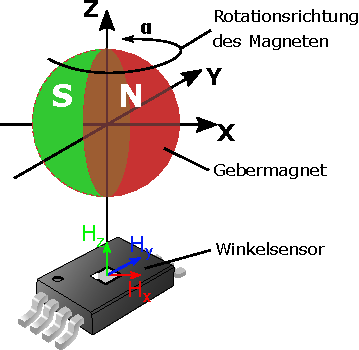
\includegraphics[width=\linewidth]{images/Klassischer_Anwendungsfall}<1-3>
	\end{figure}
\end{columns}
\end{frame}
%%%%%%%%%%%%%%%%%%%%%%%%%%%%%%%%%%%%%%%%%%%%%%%%%%%%%%%%%%%%%%%%%%%%%%%%%%%%%%%%%%%%%%%%%%%%%%%%%%%%%%%%%%%%%%%%%%%%%%%%%%%%%%%%%%%%%%%%%
\subsection{Kreisdarstellung der Winkelmessung}
\begin{frame}
\frametitle{Klassischer Anwendungsfall}
\framesubtitle{Kreisdarstellung der Winkelmessung}
\begin{columns}[c]
	\column{.5\textwidth}
	\begin{overprint}
		\onslide<2>
		\begin{block}{Radius}
			\resizebox{.6\hsize}{!}{$%
				r = |\mathbf{A}| \phantom{=\sqrt{a_x^2 + a_y^2}}%
				$}
		\end{block}
		\onslide<3->
		\begin{block}<3-4>{Radius}
			\resizebox{.6\hsize}{!}{$%
				r = |\mathbf{A}| =\sqrt{a_x^2 + a_y^2}%
				$}
		\end{block}
	\end{overprint}
	\begin{block}<4->{Winkel}
	\resizebox{\hsize}{!}{$%		
		\alpha = 
		\begin{cases}
			\text{arctan2}(a_y,a_x)        &\quad \textrm{f. } a_y > 0 \\
			\pi							   &\quad \textrm{f. } a_y = 0 \\
			\text{arctan2}(a_y,a_x) + 2\pi &\quad \textrm{f. } a_y < 0
		\end{cases}%
		$}
	\end{block}

	\column{.45\textwidth}
	\begin{figure}
		\begin{overprint}
			\onslide<1>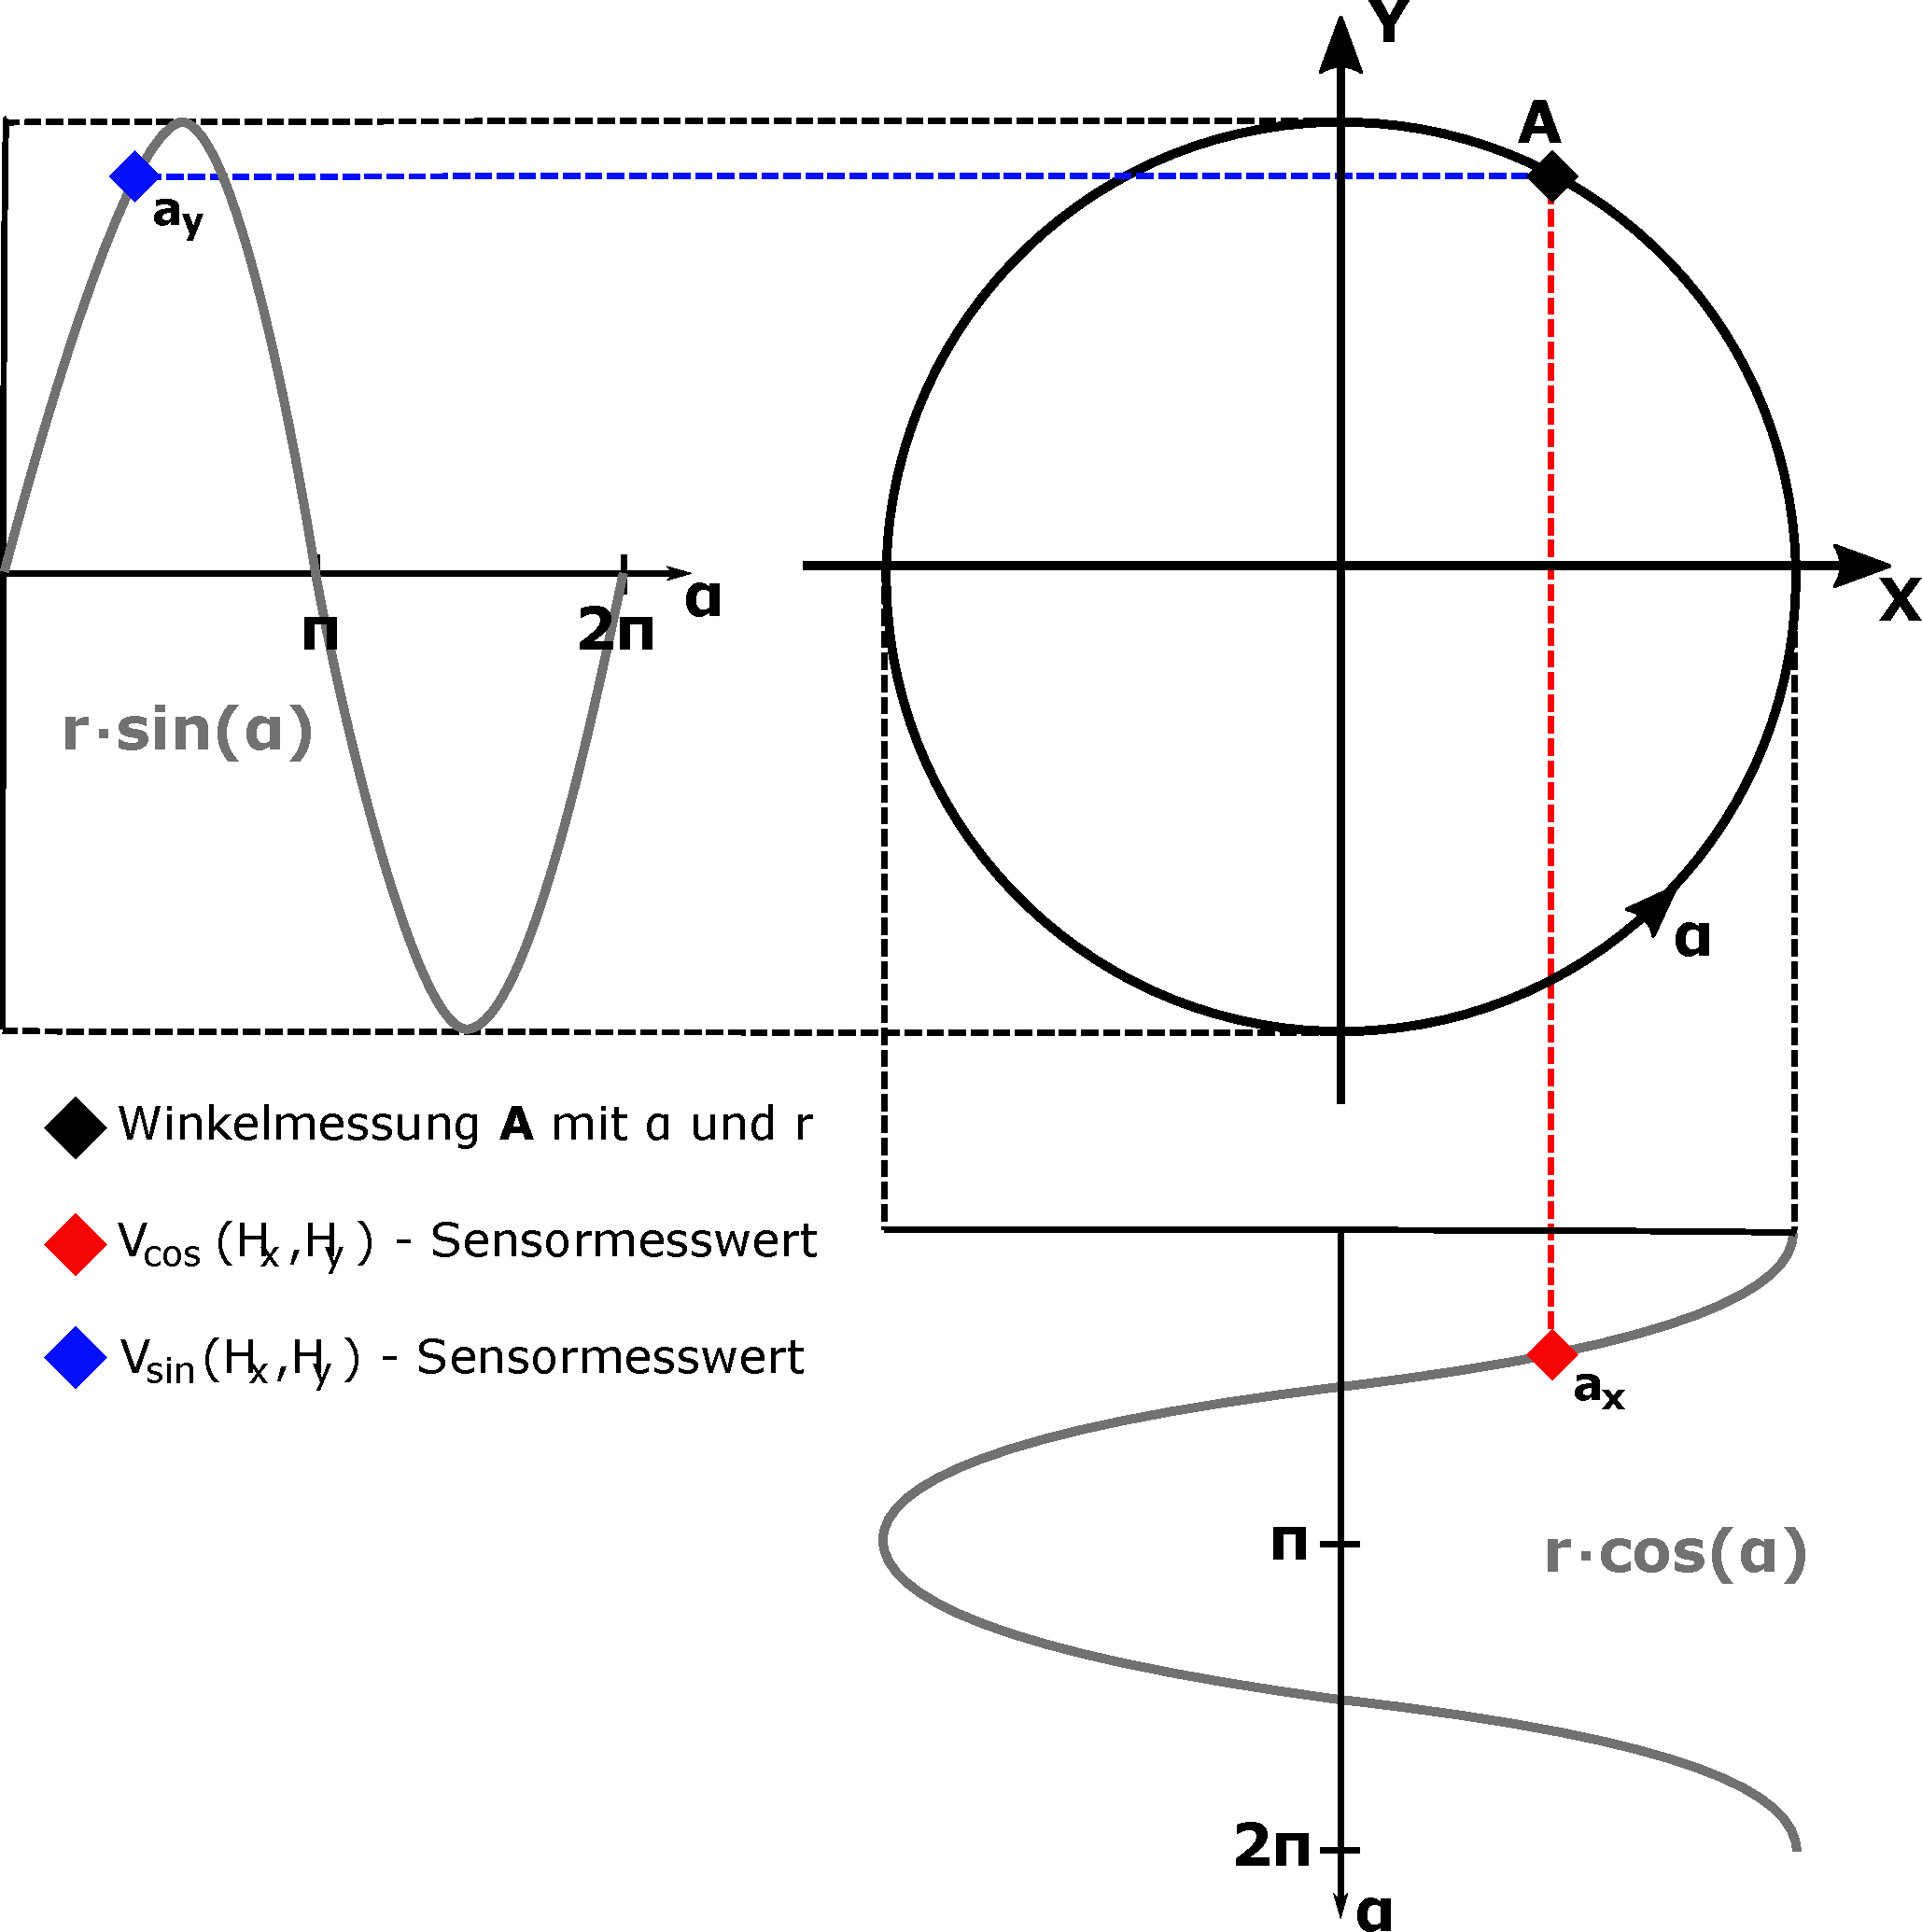
\includegraphics[width=\linewidth]{images/Kreisdarstellung_Winkelmessung-1}
			\onslide<2>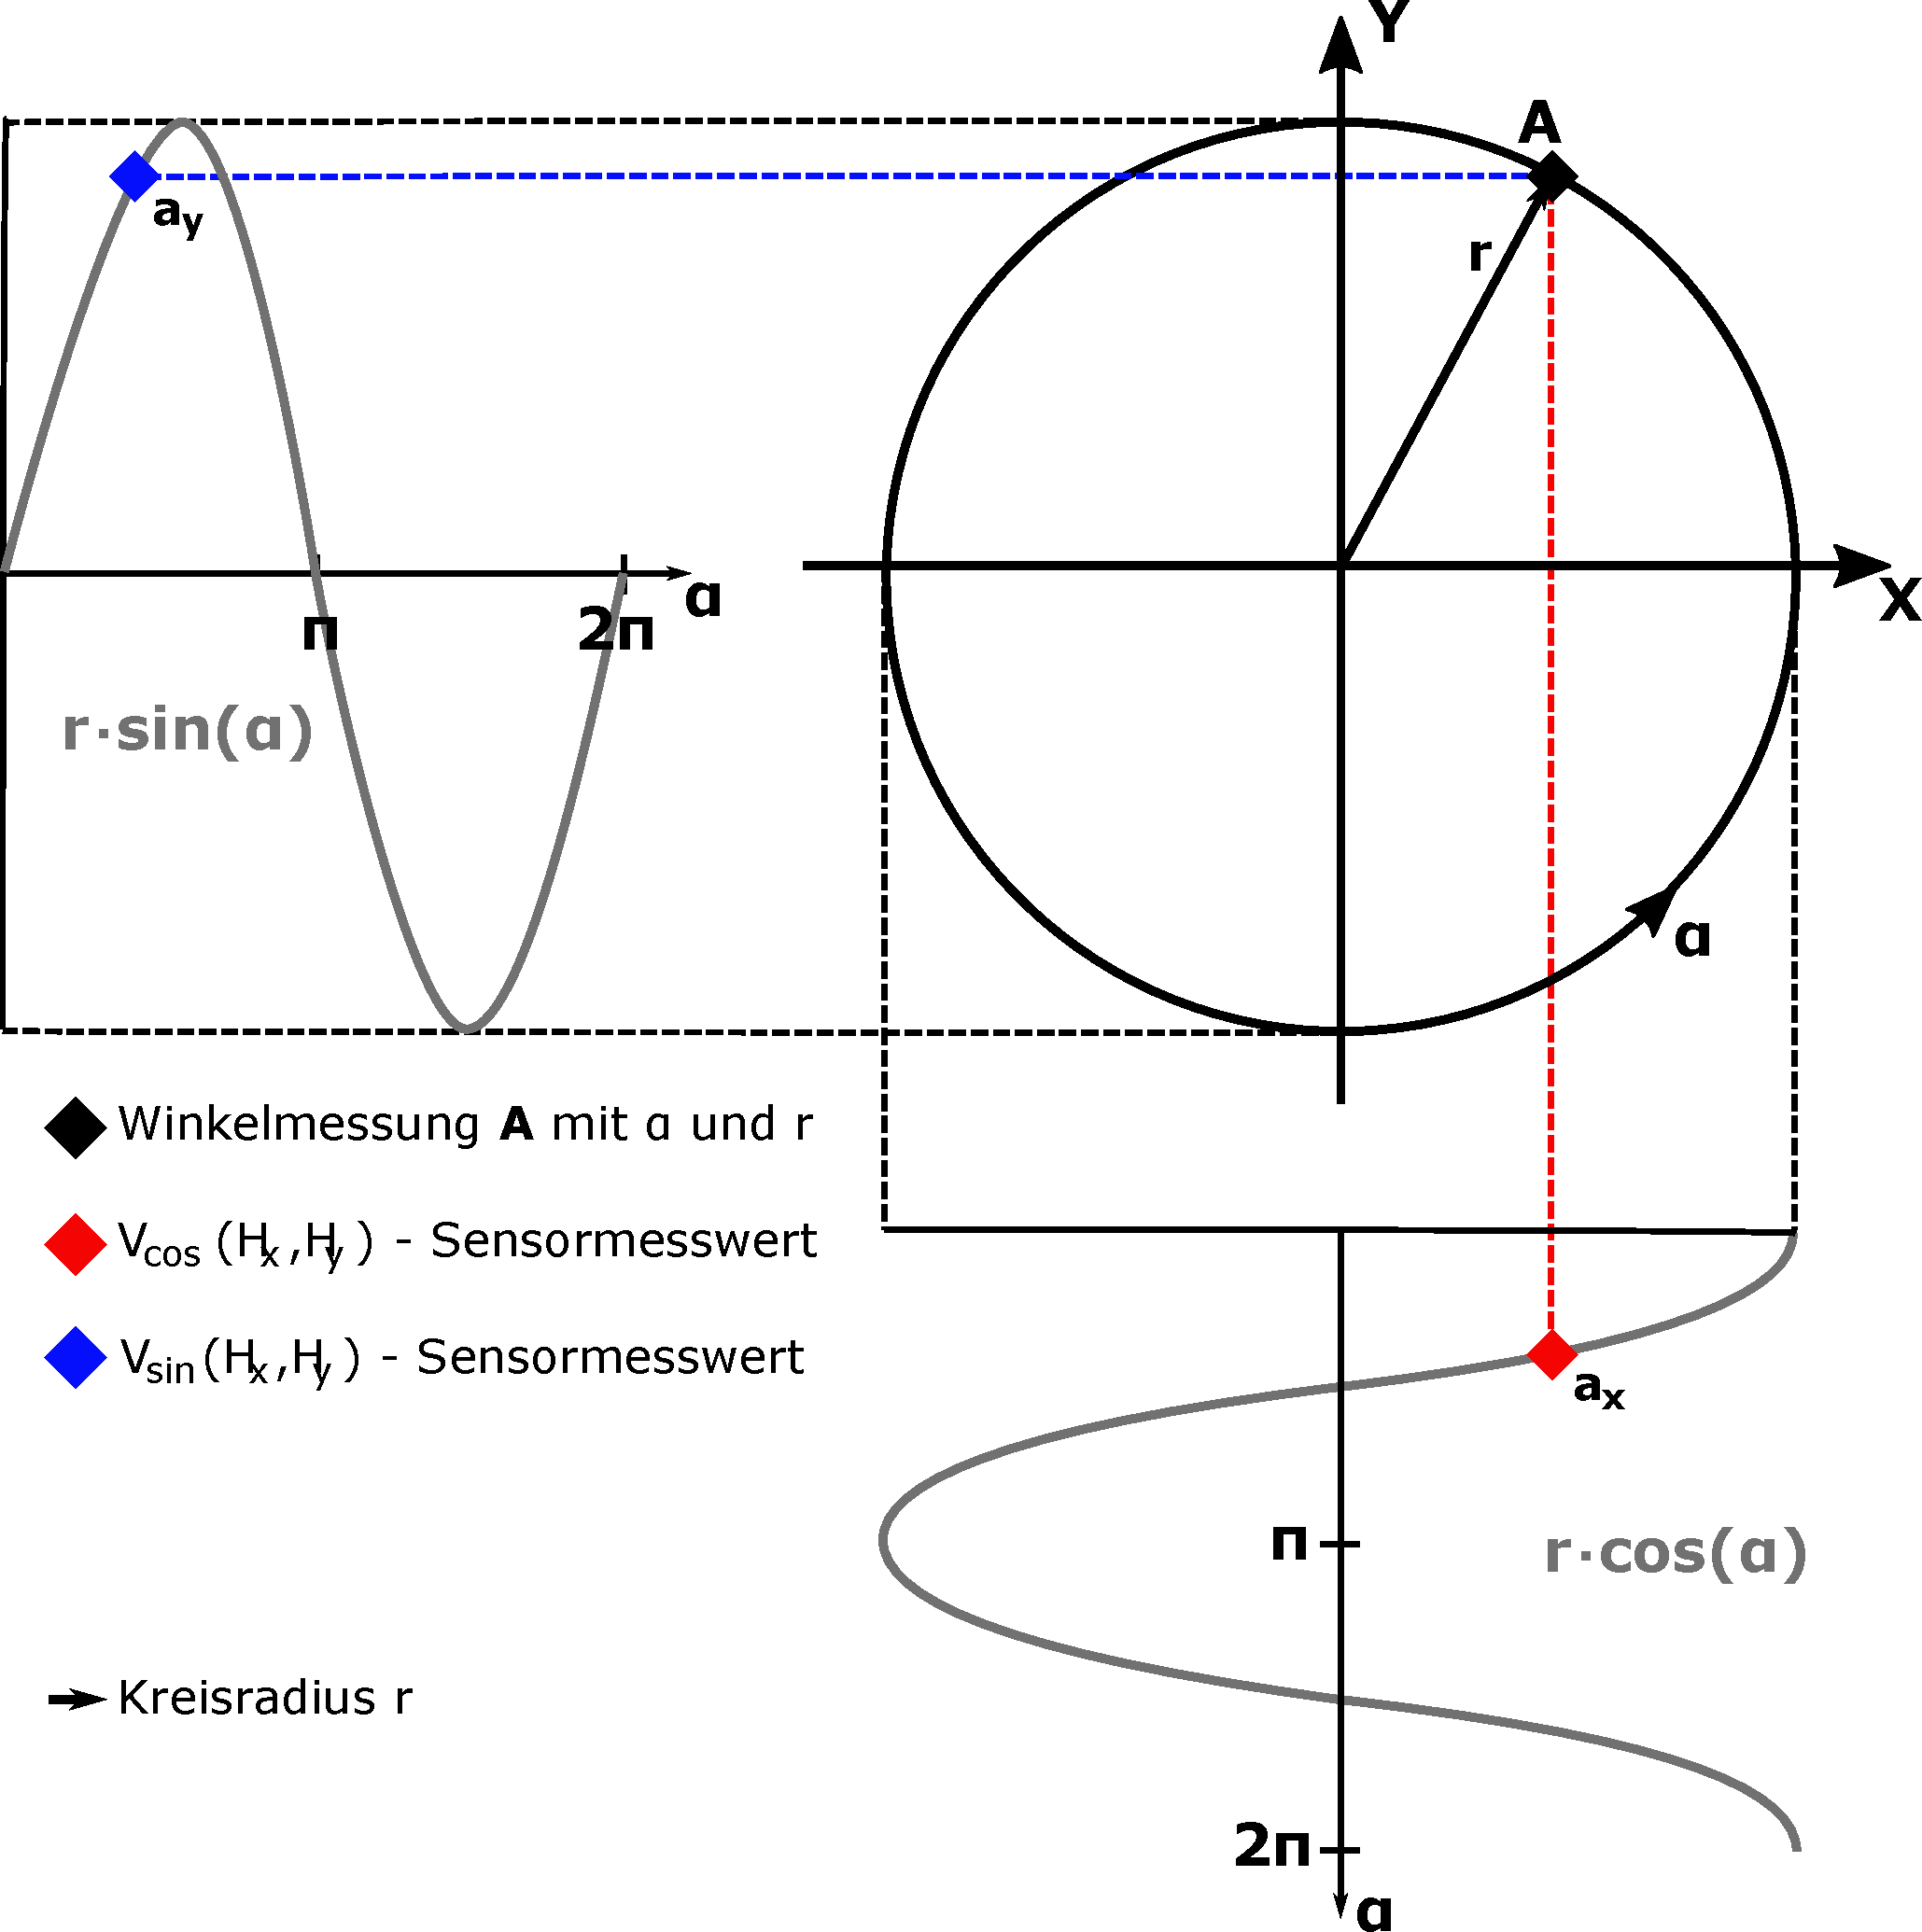
\includegraphics[width=\linewidth]{images/Kreisdarstellung_Winkelmessung-2}
			\onslide<3>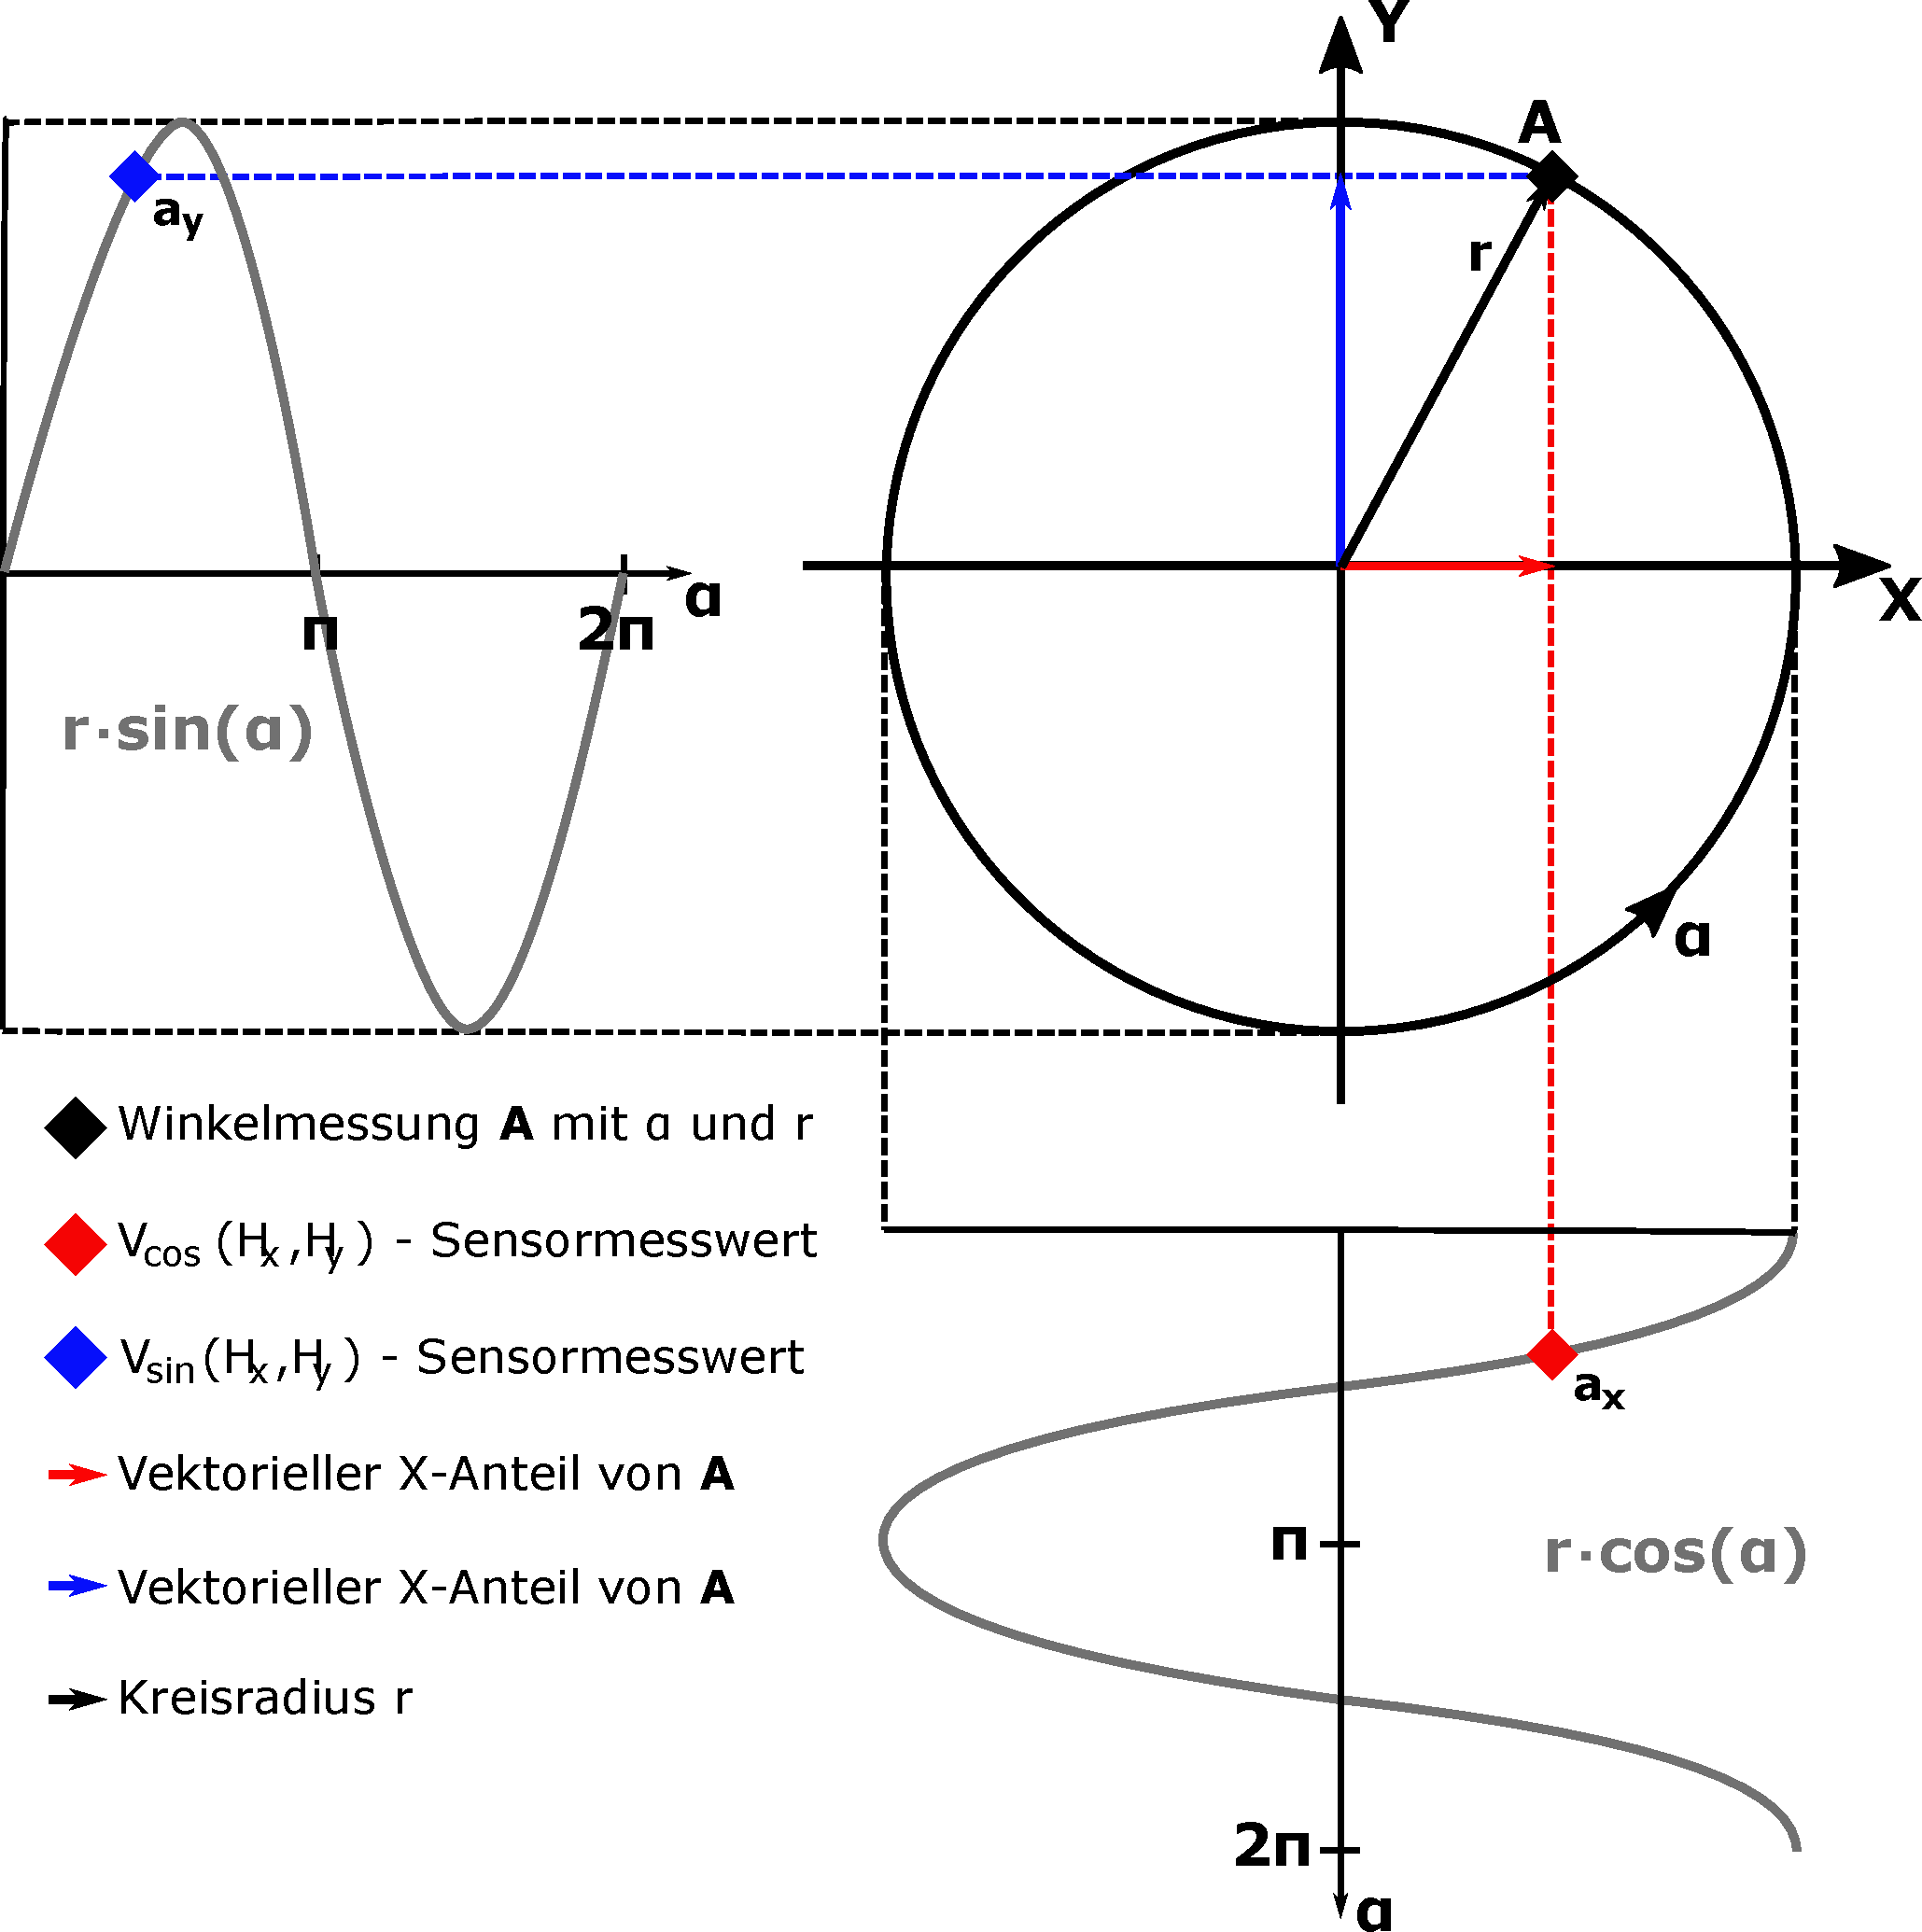
\includegraphics[width=\linewidth]{images/Kreisdarstellung_Winkelmessung-3}
			\onslide<4->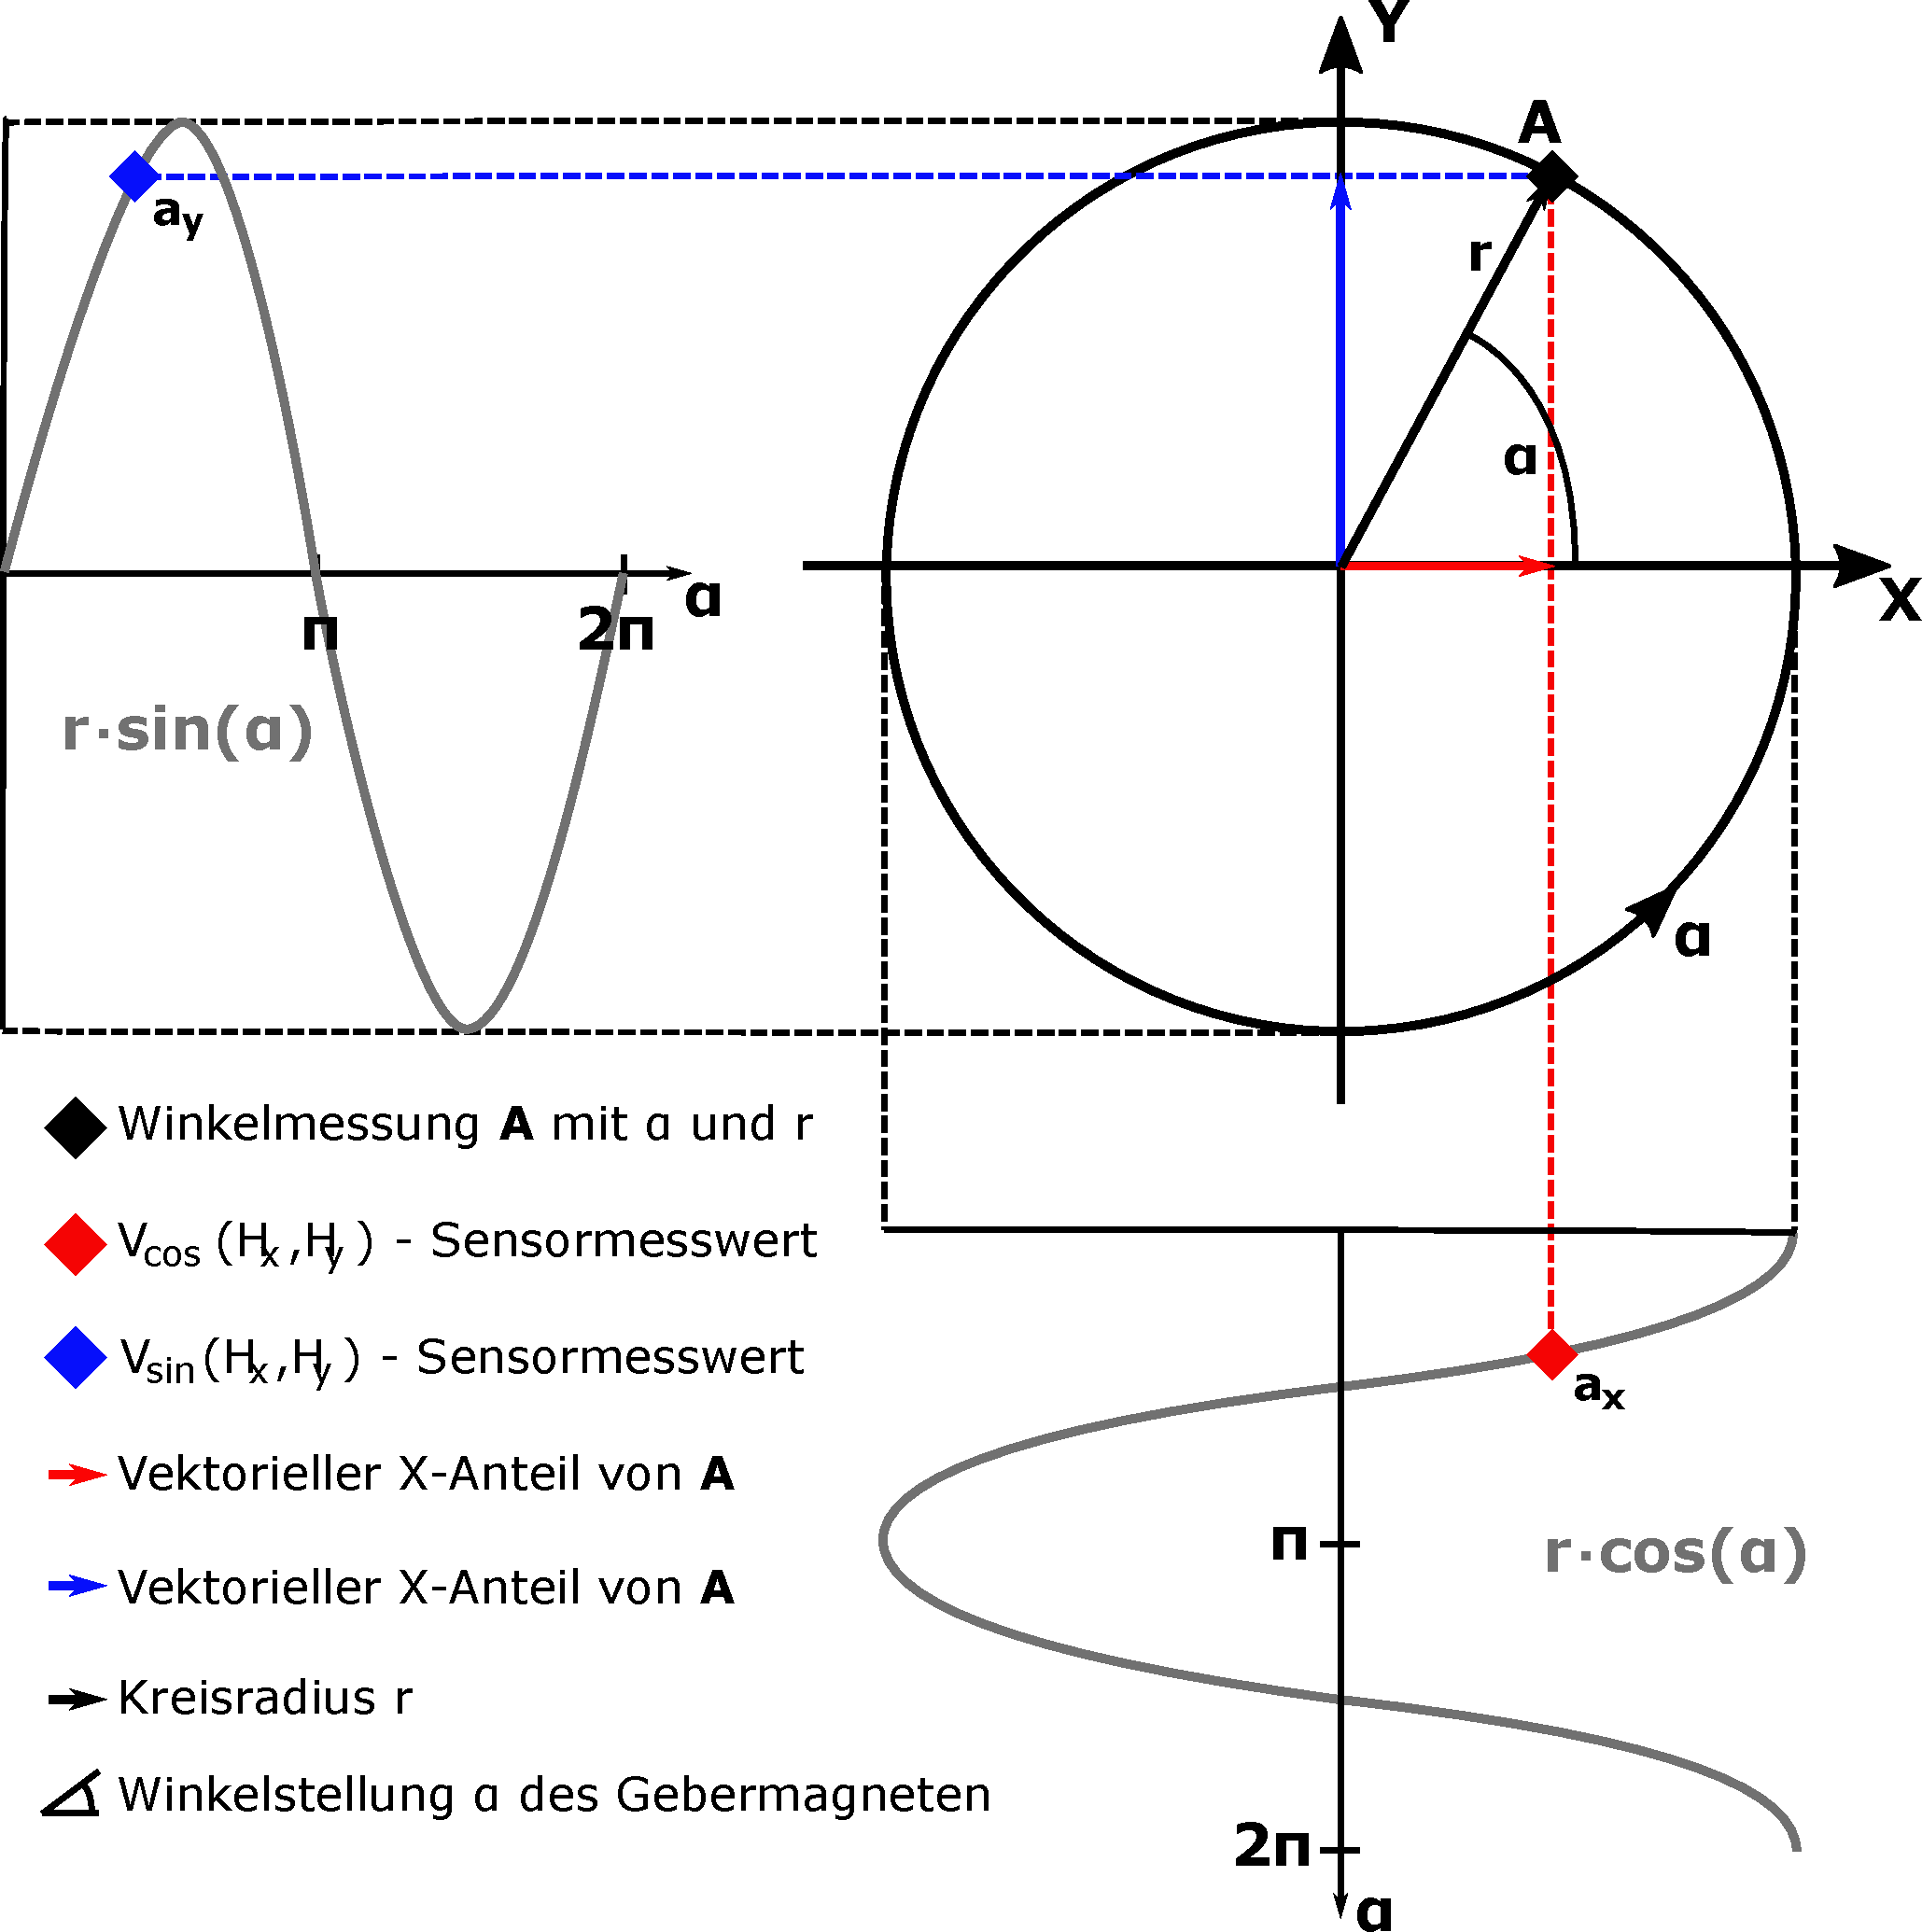
\includegraphics[width=\linewidth]{images/Kreisdarstellung_Winkelmessung}
		\end{overprint}
	\end{figure}
\end{columns}
\end{frame}
%%%%%%%%%%%%%%%%%%%%%%%%%%%%%%%%%%%%%%%%%%%%%%%%%%%%%%%%%%%%%%%%%%%%%%%%%%%%%%%%%%%%%%%%%%%%%%%%%%%%%%%%%%%%%%%%%%%%%%%%%%%%%%%%%%%%%%%%%
\subsection{Euklidischer Abstand als Winkelabstand}
\begin{frame}
\frametitle{Klassischer Anwendungsfall}
\framesubtitle{Euklidischer Abstand als Winkelabstand}
\begin{columns}[c]
	\column{.40\textwidth}
	\begin{block}<1->{Winkelmessungen}
		\resizebox{.5\hsize}{!}{$%
			\mathbf{A}\mapsto\alpha_1 \quad \mathbf{B}\mapsto\alpha_2%
			$}
	\end{block}
	\begin{block}<2->{Radius}
		\resizebox{.6\hsize}{!}{$%
			r = |\mathbf{A}| = |\mathbf{B}| = konst.%
			$}
	\end{block}
	\begin{overprint}
		\onslide<3>
		\begin{block}{Euklidischer Abstand}
			\resizebox{\hsize}{!}{$%
				d_E\langle\mathbf{A},\mathbf{B}\rangle = \phantom{\sqrt{(a_x - b_x)^2 + (a_y - b_y)^2}}%
				$}
		\end{block}
		\onslide<4>
		\begin{block}{Euklidischer Abstand}
			\resizebox{\hsize}{!}{$%
				d_E\langle\mathbf{A},\mathbf{B}\rangle = \sqrt{(a_x - b_x)^2 \phantom{+ (a_y - b_y)^2}}%
				$}
		\end{block}
		\onslide<5>
		\begin{block}{Euklidischer Abstand}
			\resizebox{\hsize}{!}{$%
				d_E\langle\mathbf{A},\mathbf{B}\rangle = \sqrt{(a_x - b_x)^2 \phantom{+} (a_y - b_y)^2}%
				$}
		\end{block}
		\onslide<6>
		\begin{block}{Euklidischer Abstand}
			\resizebox{\hsize}{!}{$%
				d_E\langle\mathbf{A},\mathbf{B}\rangle = \sqrt{(a_x - b_x)^2 + (a_y - b_y)^2}%
				$}
		\end{block}
		\begin{block}{Abstandsquadrat}
			\resizebox{\hsize}{!}{$%
				d_E^2\langle\mathbf{A},\mathbf{B}\rangle = (a_x - b_x)^2 + (a_y - b_y)^2%
				$}
		\end{block}
	\end{overprint}

	\column{.55\textwidth}
	\begin{figure}
		\begin{overprint}
			\onslide<1-2>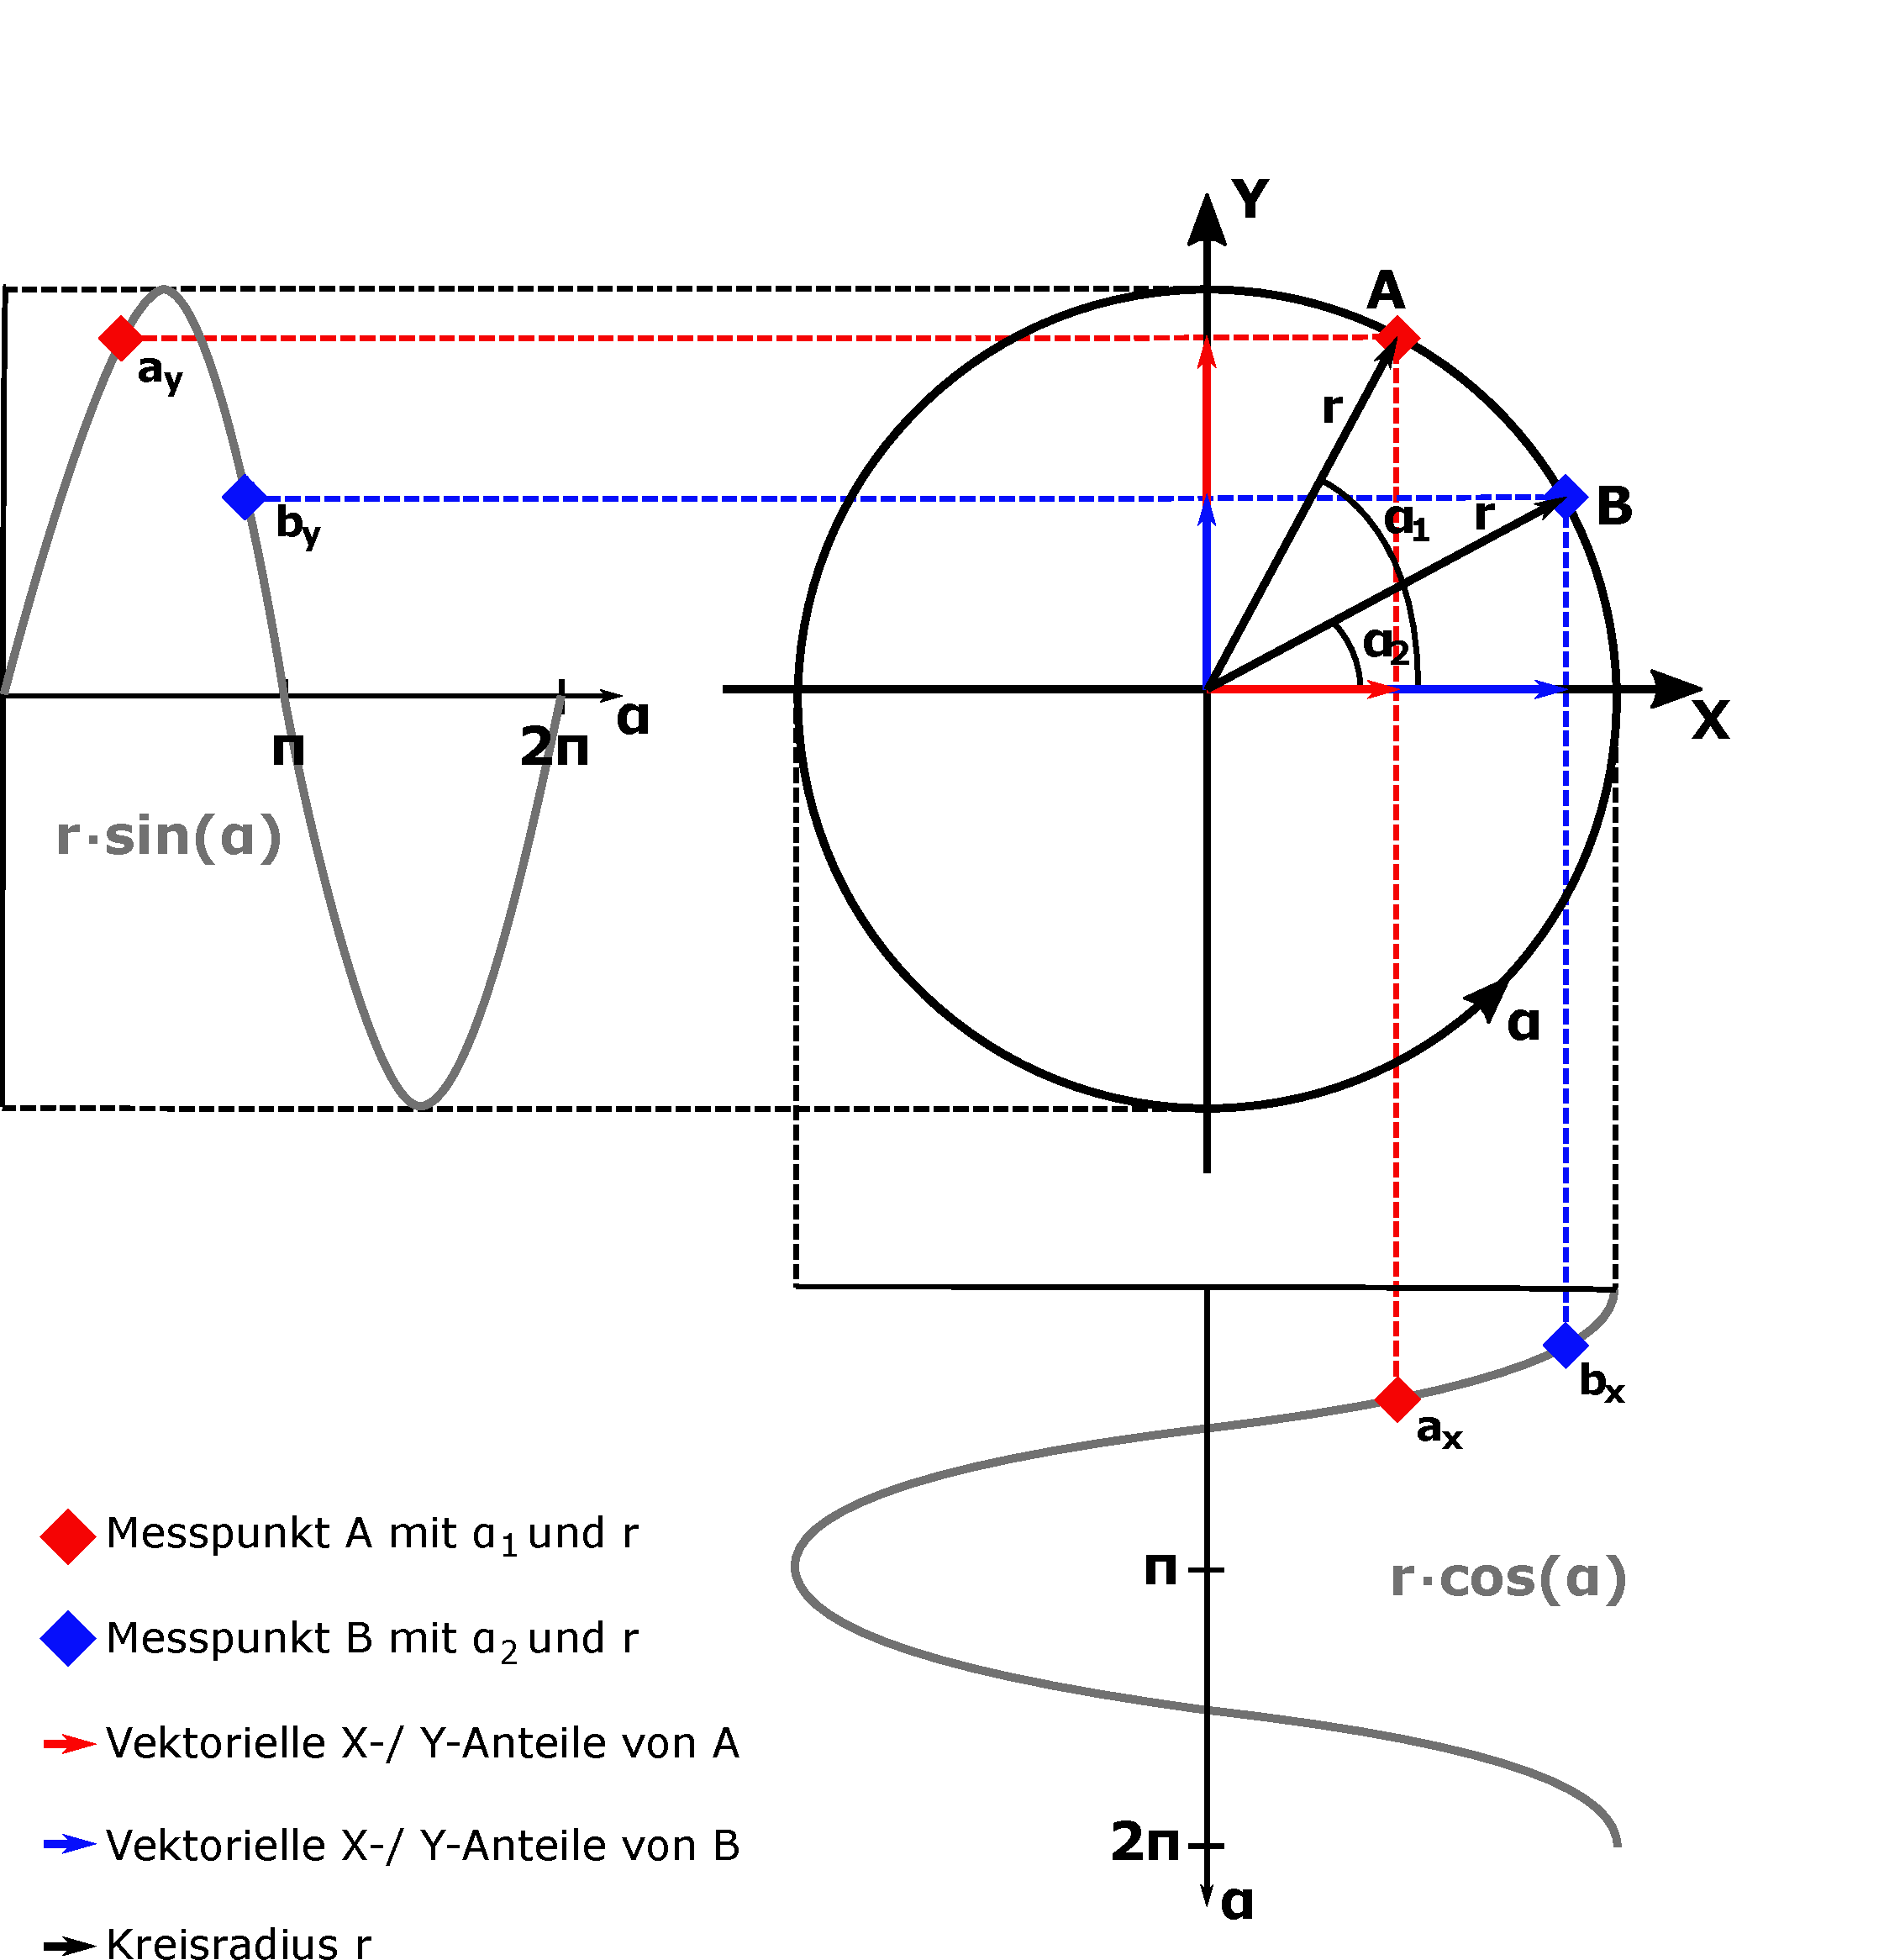
\includegraphics[width=\linewidth]{images/Kreisdarstellung_Winkelabstand-1}
			\onslide<3>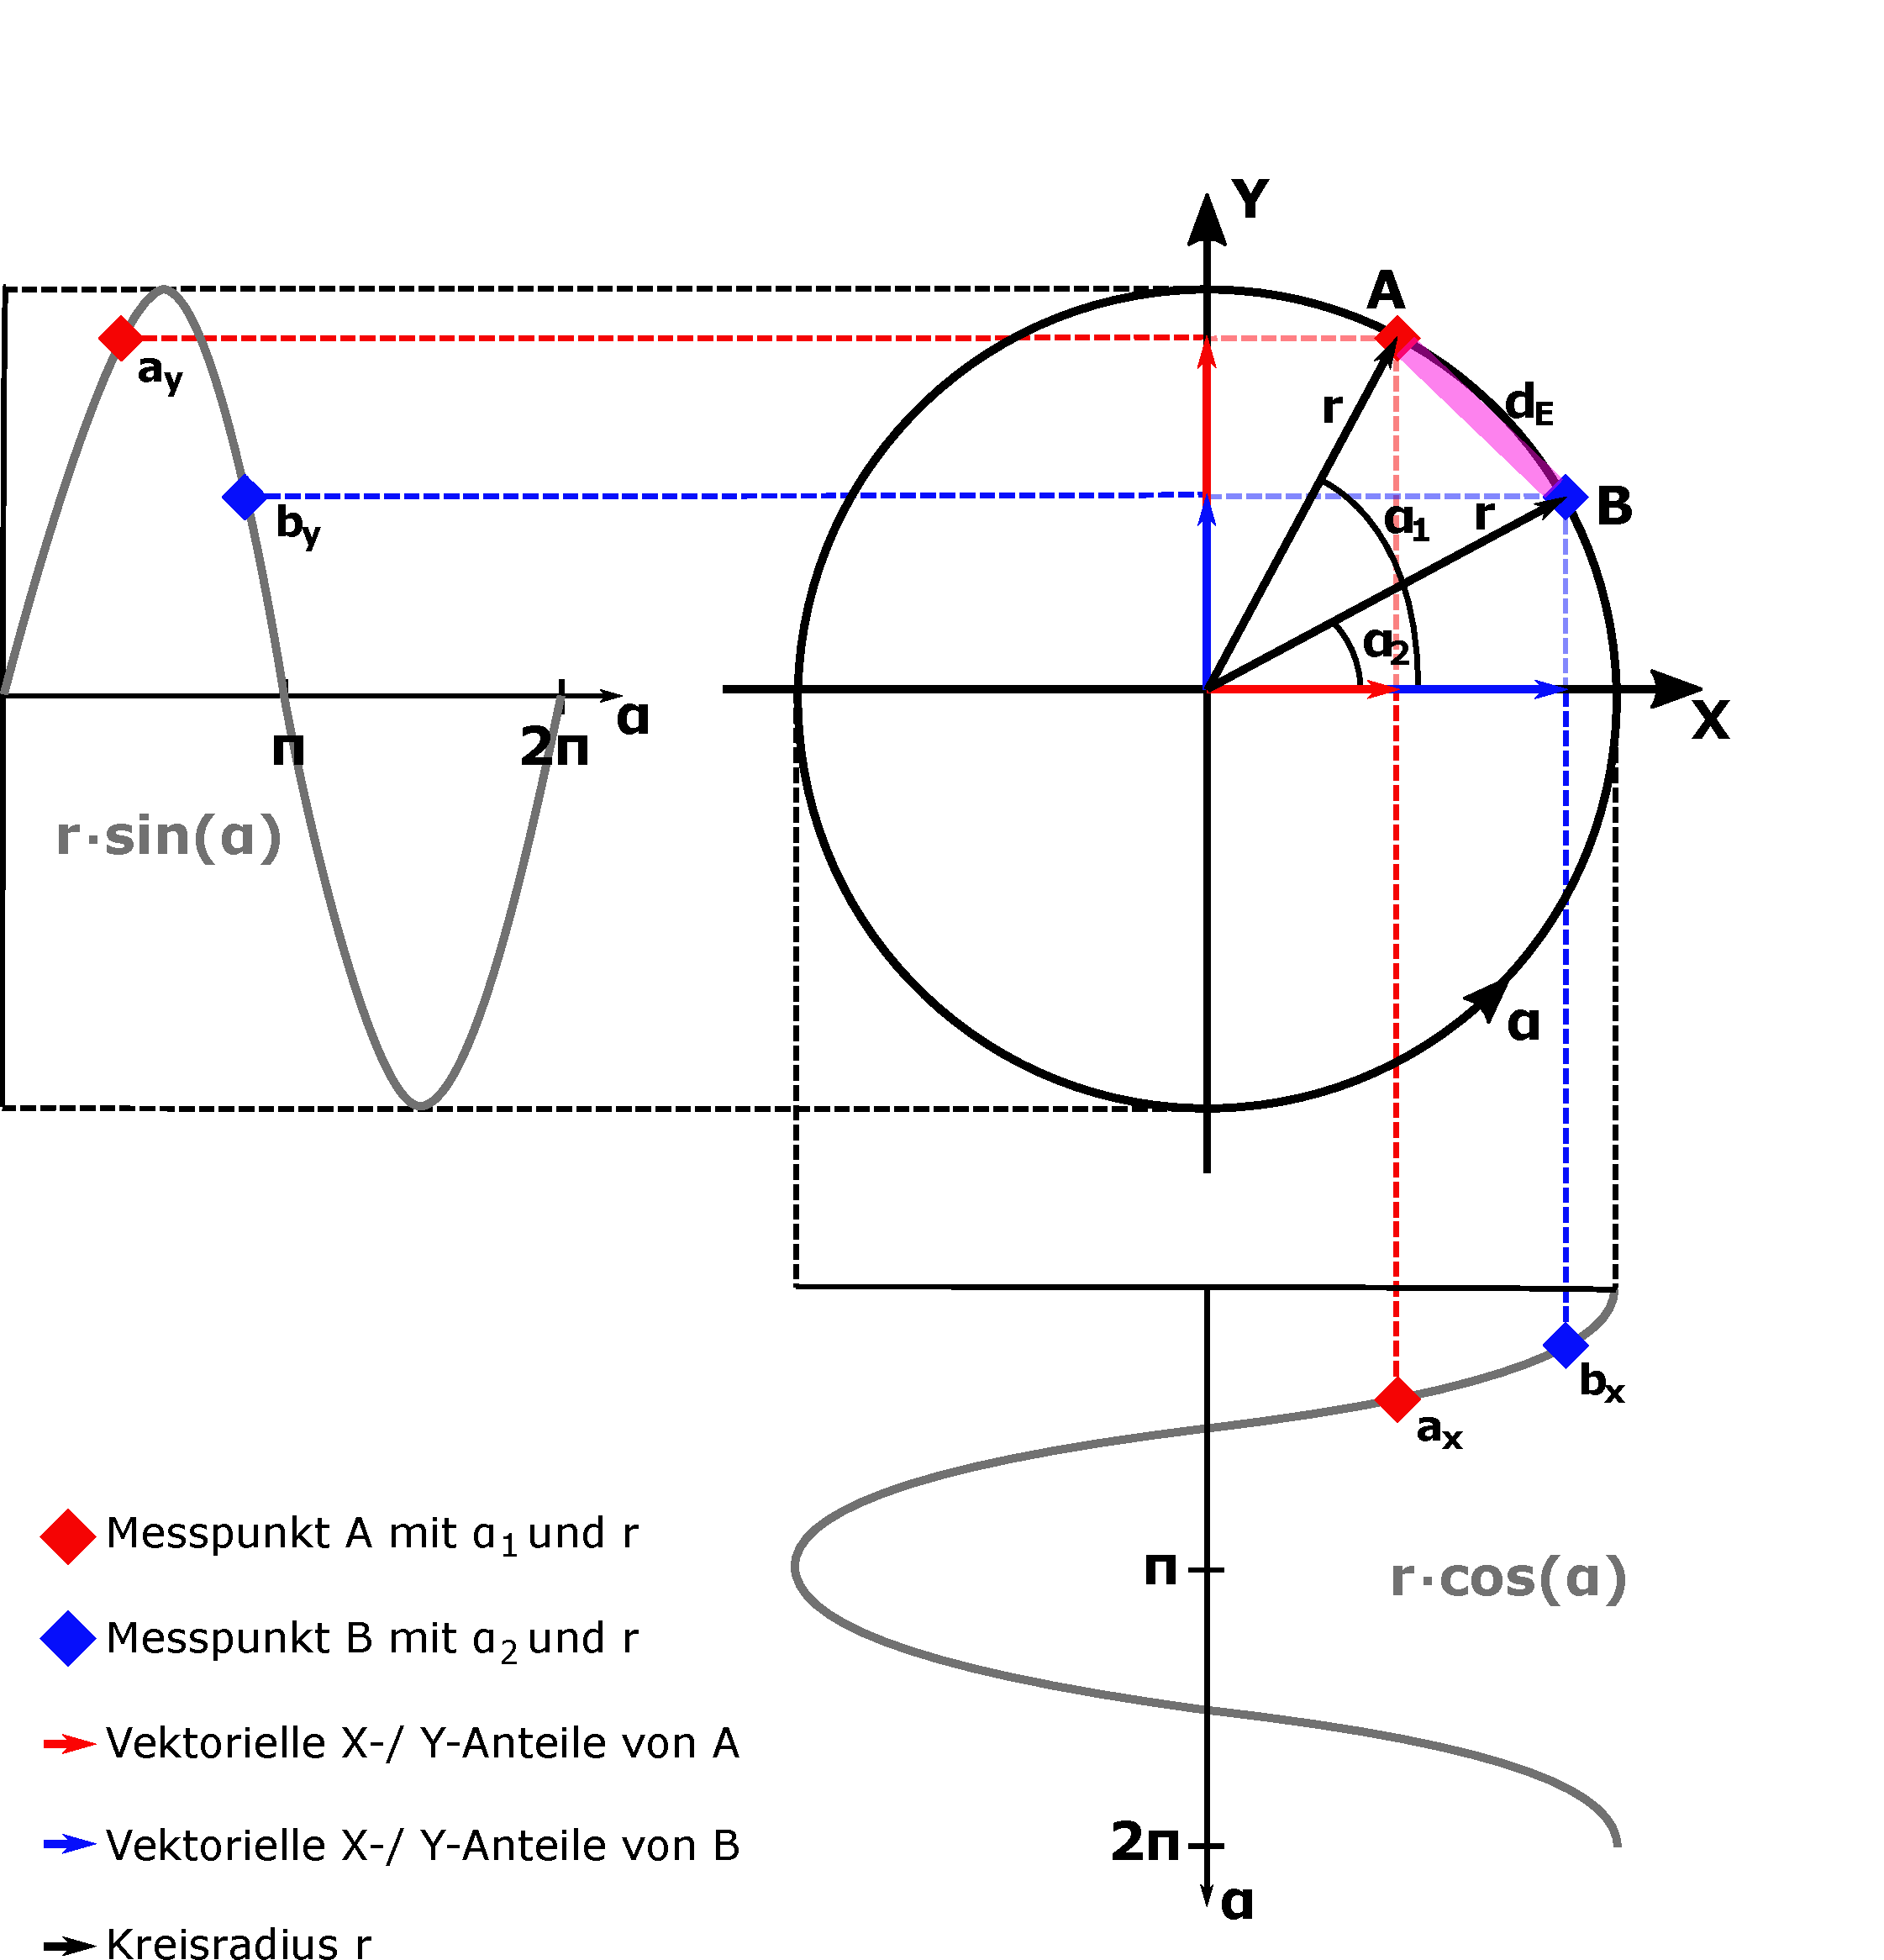
\includegraphics[width=\linewidth]{images/Kreisdarstellung_Winkelabstand-2}
			\onslide<4>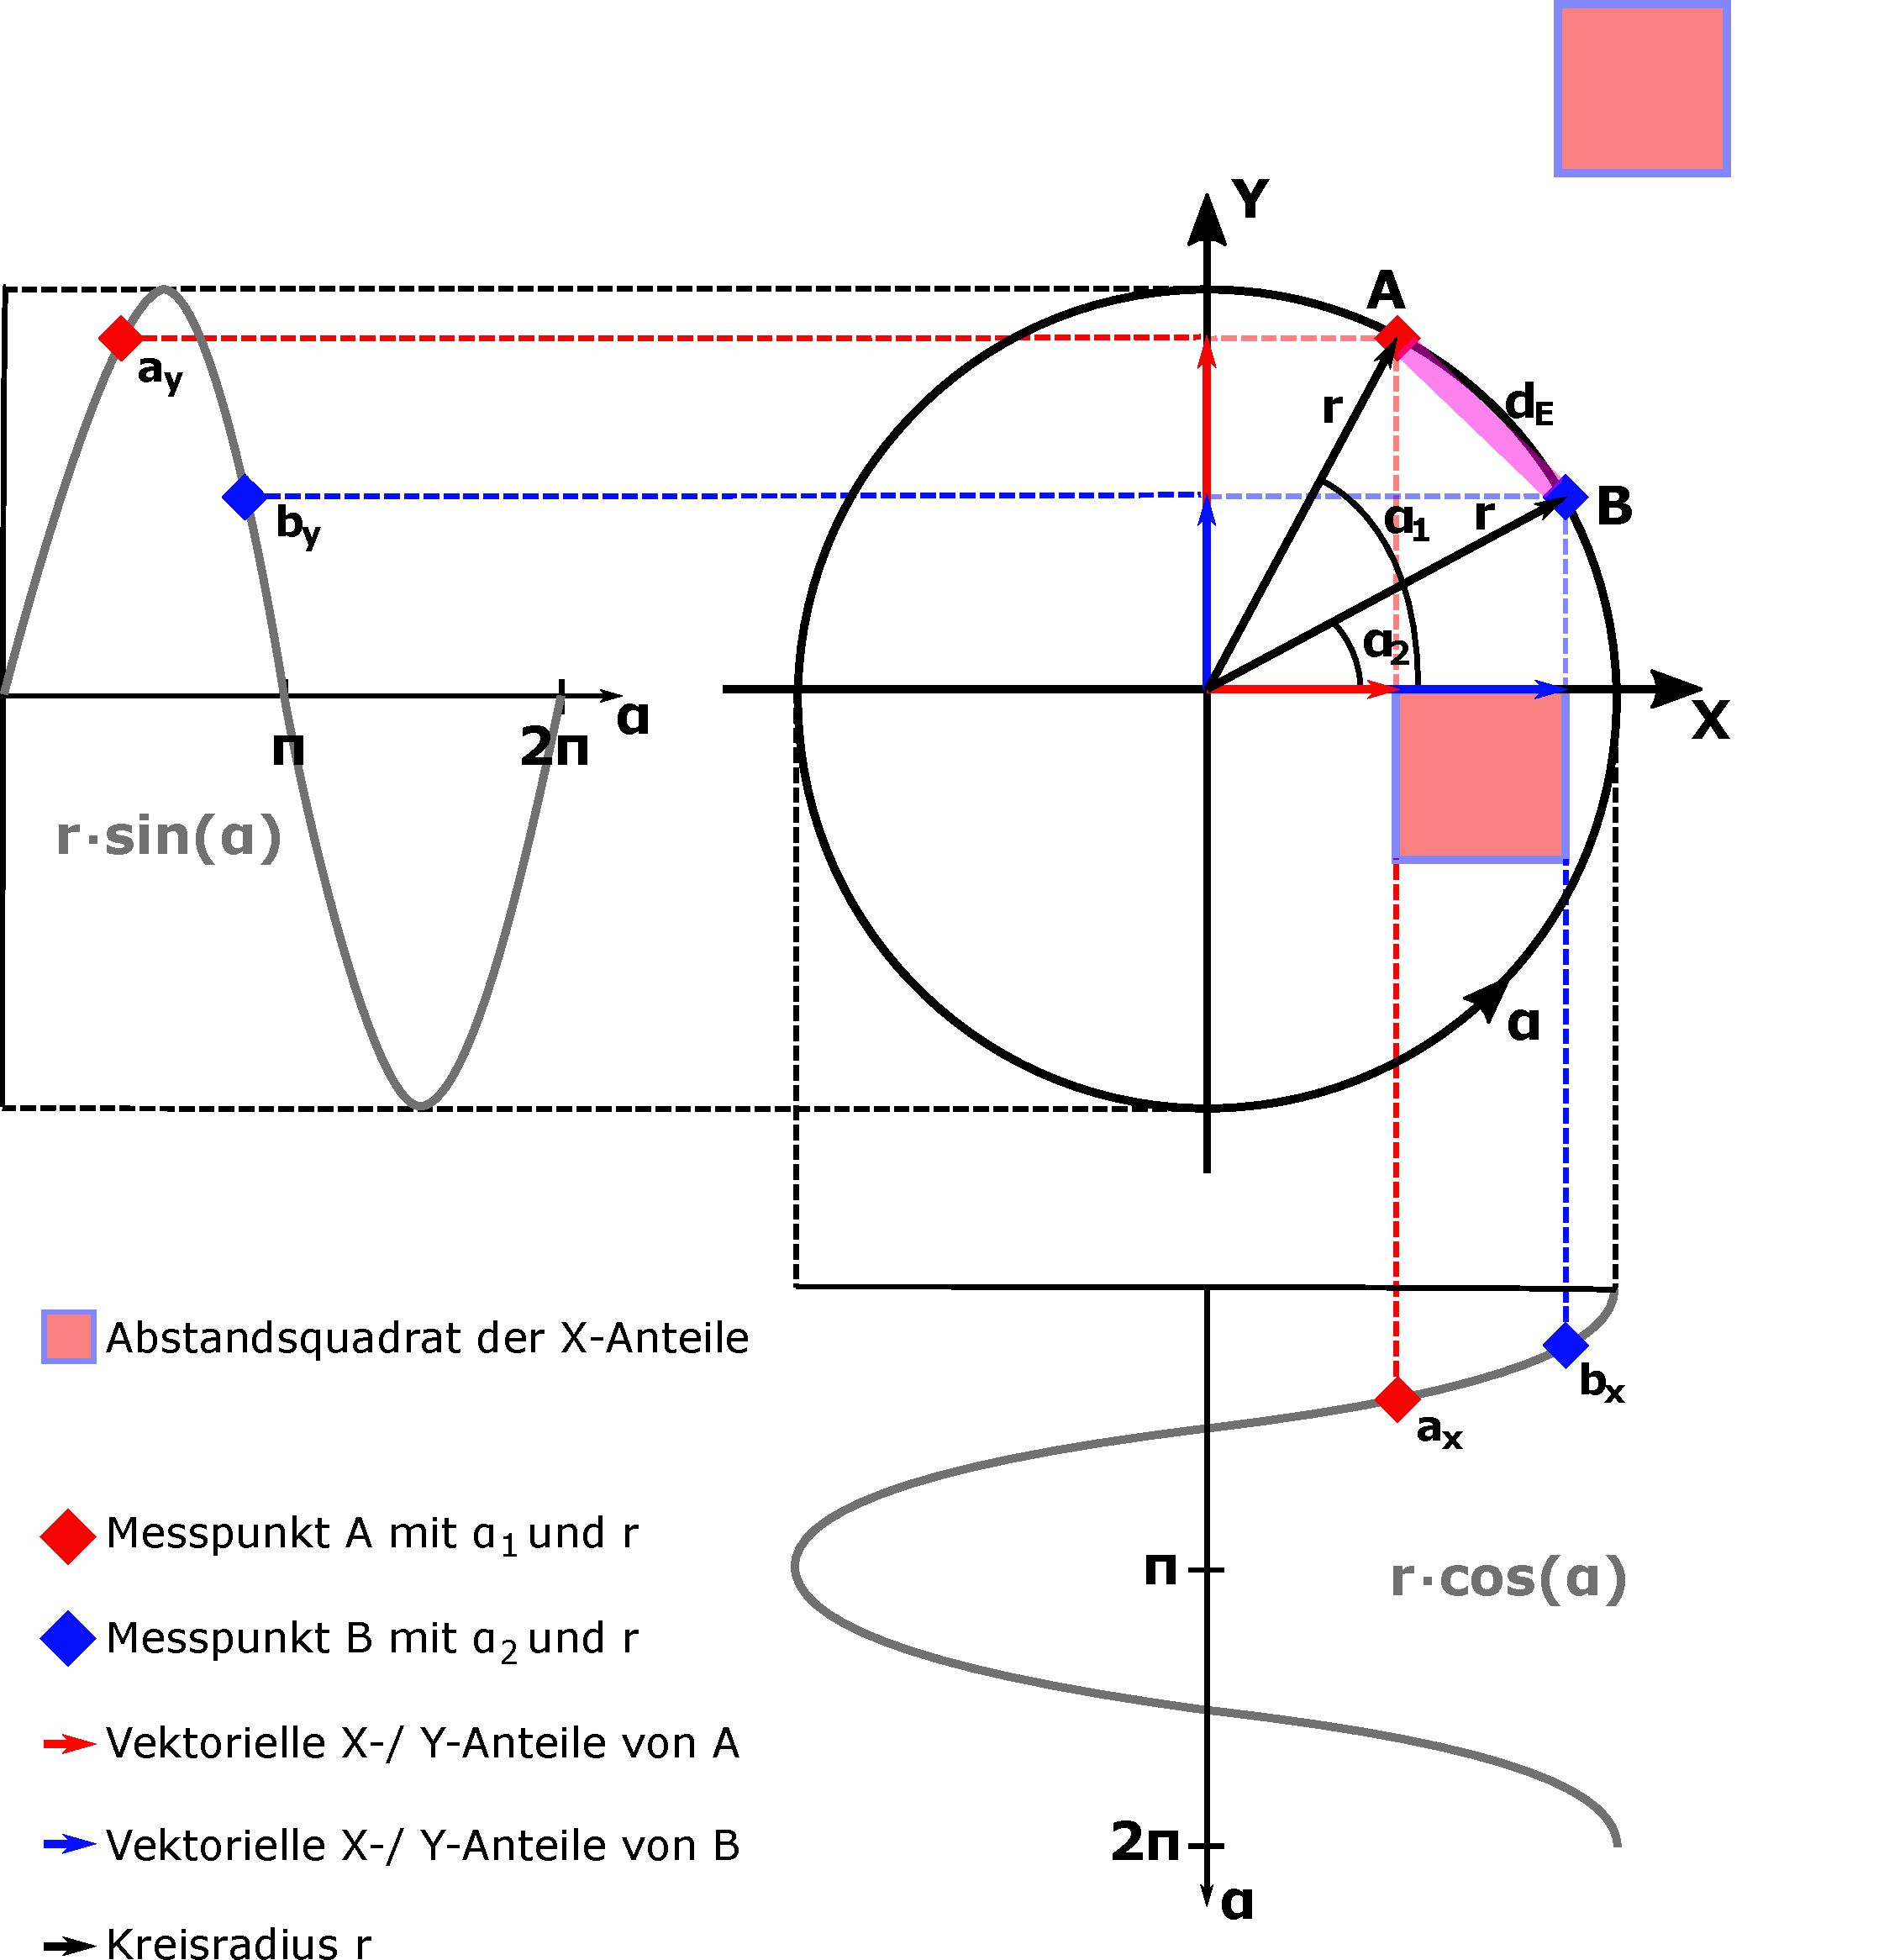
\includegraphics[width=\linewidth]{images/Kreisdarstellung_Winkelabstand-3}
			\onslide<5>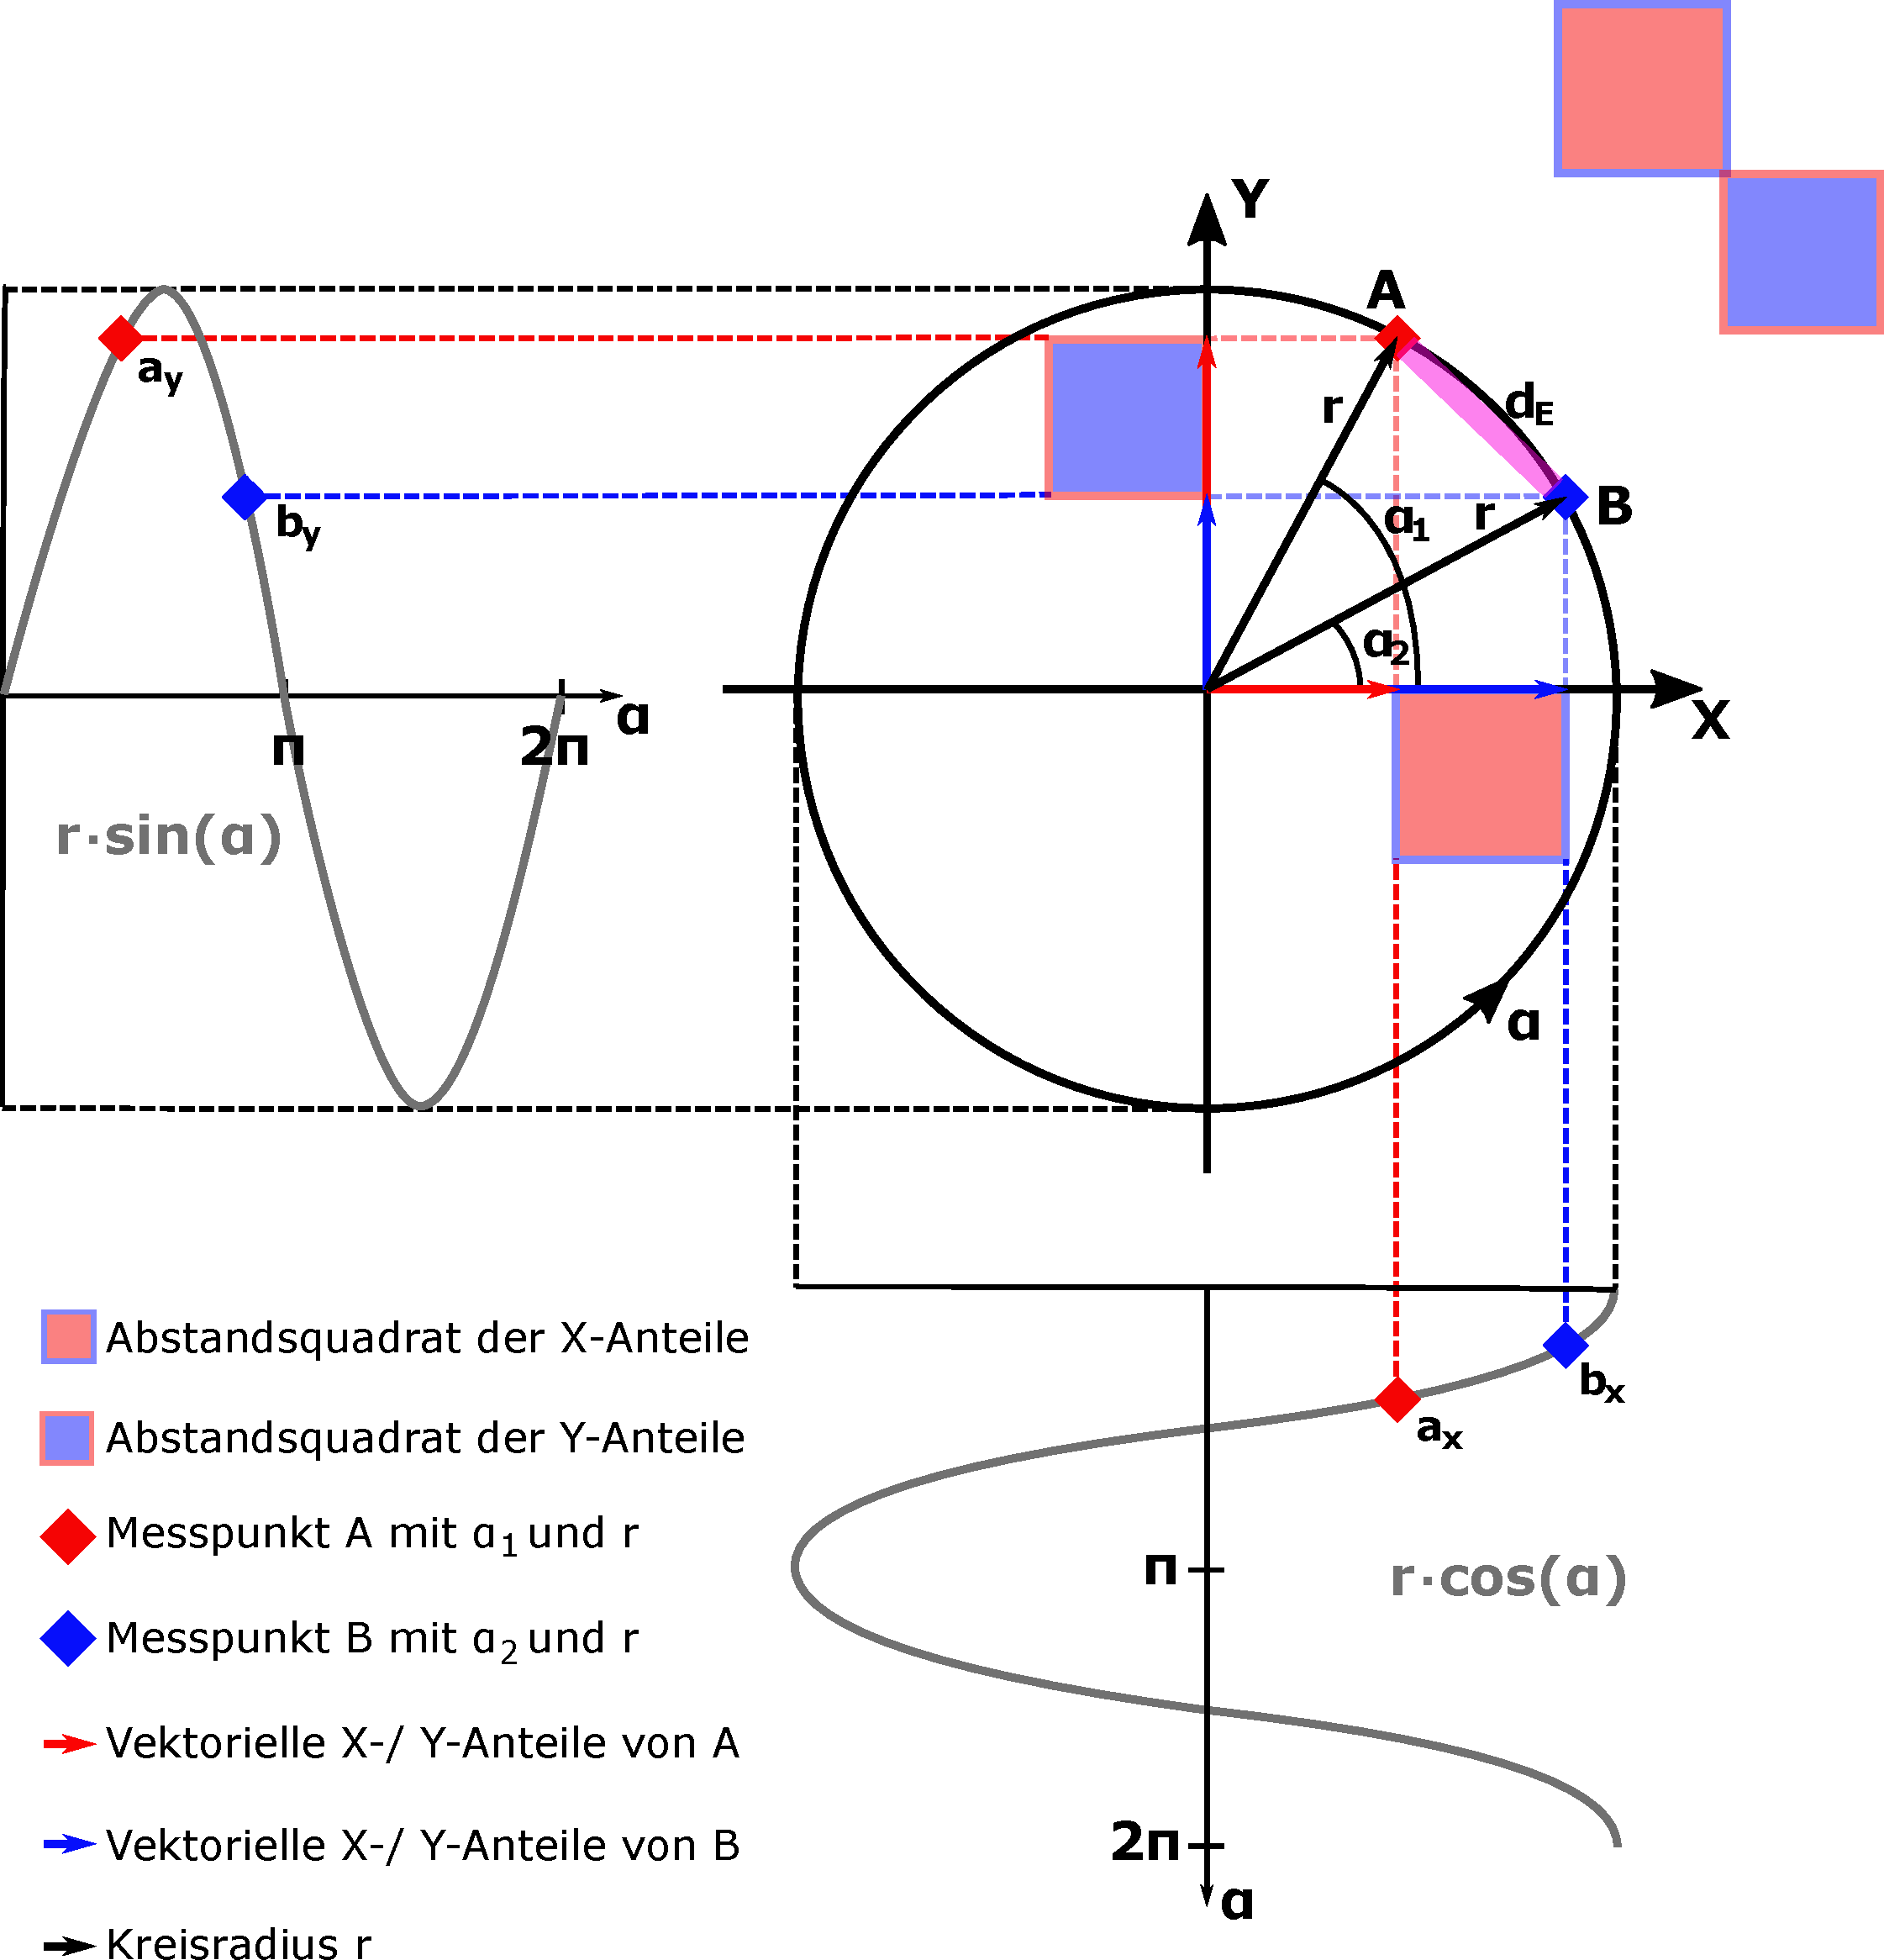
\includegraphics[width=\linewidth]{images/Kreisdarstellung_Winkelabstand-4}
			\onslide<6->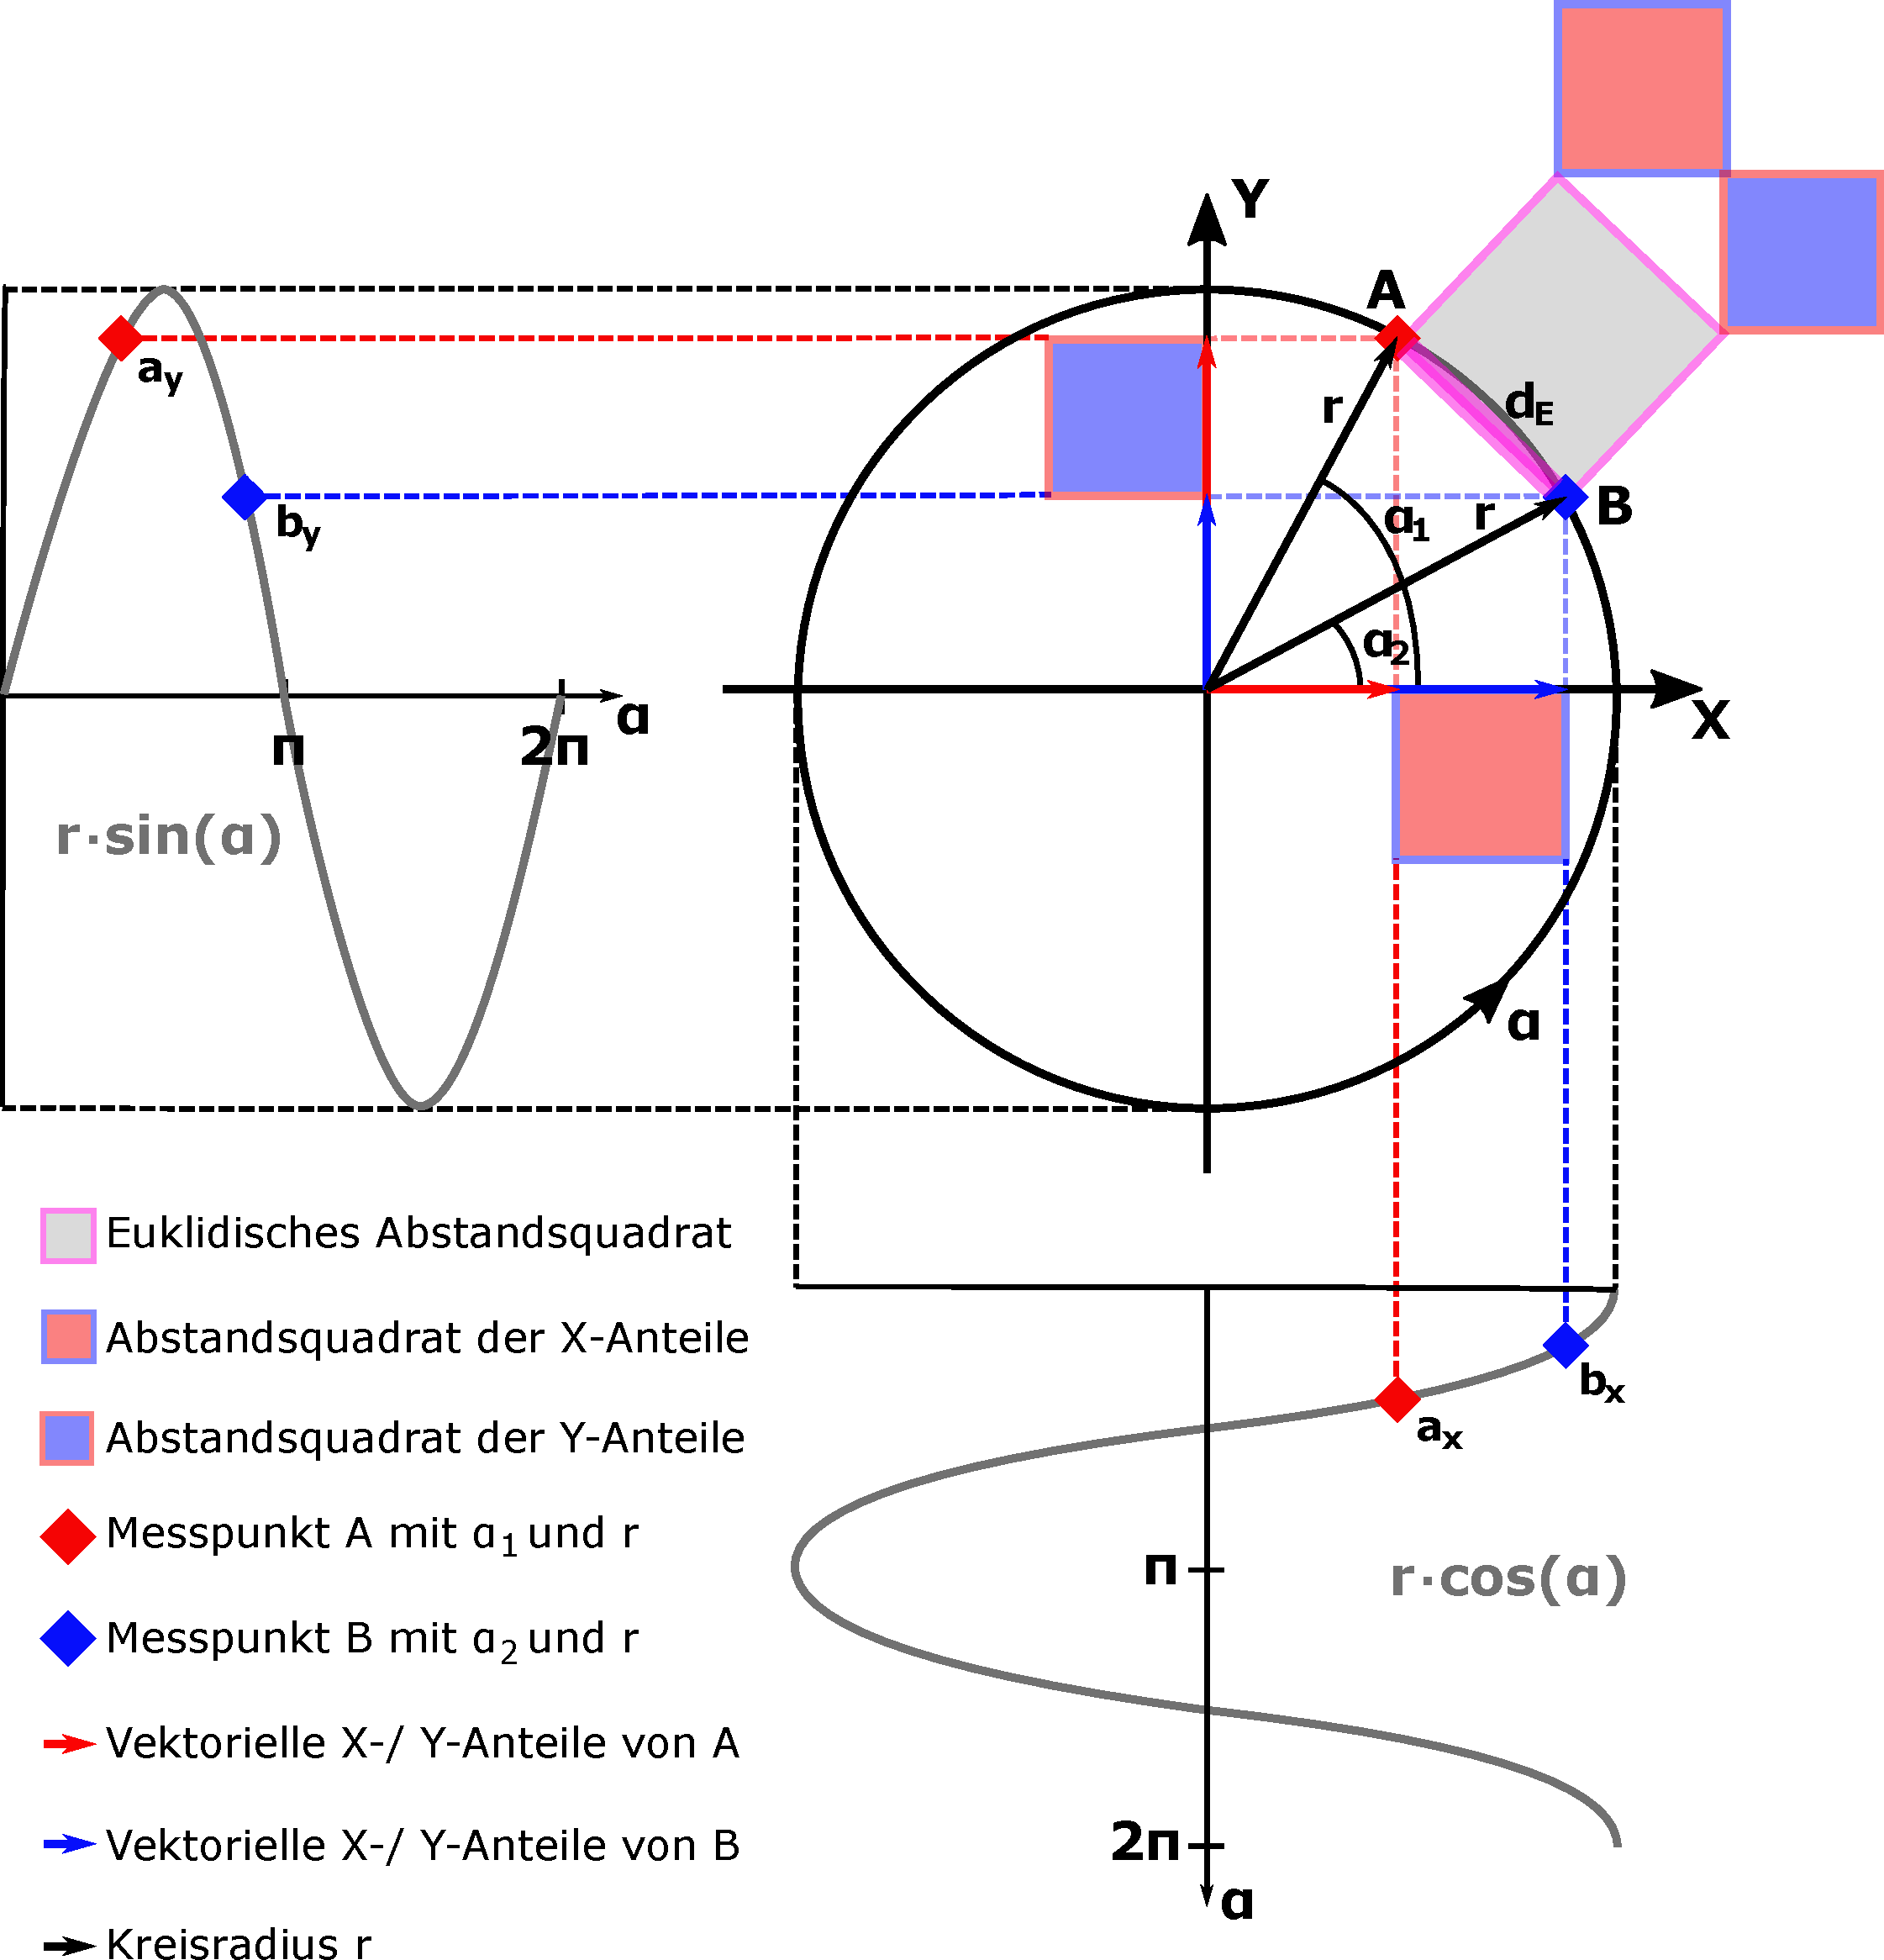
\includegraphics[width=\linewidth]{images/Kreisdarstellung_Winkelabstand}
		\end{overprint}
	\end{figure}
\end{columns}
\end{frame}
%%%%%%%%%%%%%%%%%%%%%%%%%%%%%%%%%%%%%%%%%%%%%%%%%%%%%%%%%%%%%%%%%%%%%%%%%%%%%%%%%%%%%%%%%%%%%%%%%%%%%%%%%%%%%%%%%%%%%%%%%%%%%%%%%%%%%%%%%
\section{Kreisdarstellung in Norm-Notation}
\subsection{Vektor-2-Norm für einfache Vektorfelder}
\begin{frame}
\frametitle{Kreisdarstellung in Norm-Notation}
\framesubtitle{Vektor-2-Norm für einfache Vektorfelder}
\begin{columns}[c]
	\column{.45\textwidth}
	\begin{itemize}
		\item<1-> Zweidimensionales Problem
		\item<2-> Vektorfeld in 1. Dimension $\mathbf{A} = \begin{pmatrix}a_x \\ a_y\end{pmatrix}$
		\item<2-> $\mathbf{A}\mapsto\alpha$ bildet 2. Dimension
		\item<3-> Beträge als Norm
		\item<4-> Abstand als Differenznorm
		\item<5-> Es gilt: Dreiecksungleichung
	\end{itemize}
	
	\column{.5\textwidth}
	\begin{block}{Radius}<3->
		\resizebox{.8\hsize}{!}{$%
			r := |\mathbf{A}| = \sqrt{\sum_{i=1}^{n}|A_i|^2} = \|\mathbf{A}\|_2%
		$}
	\end{block}
	\begin{block}{Euklidischer Abstand}<4->
		\resizebox{\hsize}{!}{$%
			d_E\langle\mathbf{A},\mathbf{B}\rangle := \sqrt{\sum_{i=1}^{n}(A_i - B_i)^2} = \|\mathbf{A} - \mathbf{B}\|_2%
			$}
	\end{block}
	\begin{block}{Dreiecksungleichung}<5->
		\resizebox{\hsize}{!}{$%
			\big|\|\mathbf{A}\|_2 - \|\mathbf{B}\|_2\big| \le \|\mathbf{A} \pm \mathbf{B}\|_2 \le \big|\|\mathbf{A}\|_2 + \|\mathbf{B}\|_2\big|%
		$}
	\end{block}
\end{columns}
\end{frame}
%%%%%%%%%%%%%%%%%%%%%%%%%%%%%%%%%%%%%%%%%%%%%%%%%%%%%%%%%%%%%%%%%%%%%%%%%%%%%%%%%%%%%%%%%%%%%%%%%%%%%%%%%%%%%%%%%%%%%%%%%%%%%%%%%%%%%%%%%
\subsection{Überführung in höheren Norm-Raum für Vektormatrizen}
\begin{frame}
\frametitle{Kreisdarstellung in Norm-Notation}
\framesubtitle{Überführung in höheren Norm-Raum für Vektormatrizen}
\begin{columns}[c]
	\column{.45\textwidth}
	\begin{itemize}
		\item<1-> Vierdimensionales Problem
		\item<2-> $1. + 2.$ Dimension durch Array-Geometrie
		\item<3-> $\mathbf{A}\mapsto\alpha$ bildet 3. Dimension
		\item<4-> Vektorfelder in 4. Dimension $\mathbf{A} = [\mathbf{A_x}, \mathbf{A_y}]$
		\item<5-> Frobenius Norm - Matrix als langer Vektor
		\item<6-> Nutzen von Ähnlichkeit
		\item<7-> Es muss Dreiecksungleichung gelten
	\end{itemize}
	
	\column{.5\textwidth}
	\begin{block}{Vektor-2-Norm${}^2$ f. $j$-te Spalte}<5->
		$\|\mathbf{A_x}\|_F= \sqrt{\sum_{j=1}^{n}\|A_{xj}\|_2^2}$
	\end{block}
	\begin{block}{Ungleichung: Vektor-2-Norm}<6->
		\resizebox{\hsize}{!}{$%
			\big|\|\mathbf{A}\|_2 - \|\mathbf{B}\|_2\big| \le \|\mathbf{A} \pm \mathbf{B}\|_2 \le \big|\|\mathbf{A}\|_2 + \|\mathbf{B}\|_2\big|%
			$}
	\end{block}
	\onslide<6->{\centering$\Downarrow$}
	\begin{block}{Ungleichung: Frobenius Norm}<7->
		\resizebox{\hsize}{!}{$%
			\big|\|\mathbf{A_x}\|_F - \|\mathbf{B_x}\|_F\big| \le \|\mathbf{A_x} \pm \mathbf{B_x}\|_F \le \big|\|\mathbf{A_x}\|_F + \|\mathbf{B_x}\|_F\big|%
			$}
	\end{block}
\end{columns}
\end{frame}
%%%%%%%%%%%%%%%%%%%%%%%%%%%%%%%%%%%%%%%%%%%%%%%%%%%%%%%%%%%%%%%%%%%%%%%%%%%%%%%%%%%%%%%%%%%%%%%%%%%%%%%%%%%%%%%%%%%%%%%%%%%%%%%%%%%%%%%%%
\begin{frame}
\frametitle{Kreisdarstellung in Norm-Notation}
\framesubtitle{Überführung in höheren Norm-Raum für Vektormatrizen}

\begin{columns}[c]
	\column{.5\textwidth}
	\begin{itemize}
		\item <2-> Einsetzen v. Einzelnormen, "runter brechen" d. Komplexität
		\item <3-> Neue normierte Kreisbahn $\|r\|_F$
	\end{itemize}

	\column{.5\textwidth}
	\begin{itemize}
		\item <4-> Dreiecksungleichung
		\item <5-> Vergleich der Einzelkreisbahnen $r_{i,j}$ f. $d_F^2\langle\mathbf{A},\mathbf{B}\rangle$
	\end{itemize}
\end{columns}

\begin{overprint}
\onslide<1>
\begin{block}{Aufbau über euklidischen Abstand}
	\begin{align*}
	d_E^2\langle\mathbf{A},\mathbf{B}\rangle &= \phantom{\big(\|\mathbf{A_x}\|_F - \|\mathbf{B_x}\|_F\big)^2 + \big(\|\mathbf{A_y}\|_F - \|\mathbf{B_y}\|_F\big)^2} \\
	                                         &\phantom{\le} \nonumber \\
	d_F^2\langle\mathbf{A},\mathbf{B}\rangle &= \phantom{\|\mathbf{A_x} - \mathbf{B_x}\|_F^2 + \|\mathbf{A_y} - \mathbf{B_y}\|_F^2 = \|\mathbf{A} - \mathbf{B}\|_F^2}
	\end{align*}%
\end{block}
\onslide<2-3>
\begin{block}{Aufbau über euklidischen Abstand}
	\begin{align*}
	d_E^2\langle\mathbf{A},\mathbf{B}\rangle &= \big(\|\mathbf{A_x}\|_F - \|\mathbf{B_x}\|_F\big)^2 + \big(\|\mathbf{A_y}\|_F - \|\mathbf{B_y}\|_F\big)^2 \\
											 &\phantom{\le} \nonumber \\
	d_F^2\langle\mathbf{A},\mathbf{B}\rangle &= \phantom{\|\mathbf{A_x} - \mathbf{B_x}\|_F^2 + \|\mathbf{A_y} - \mathbf{B_y}\|_F^2 = \|\mathbf{A} - \mathbf{B}\|_F^2}
	\end{align*}%
\end{block}
\onslide<4>
\begin{block}{Aufbau über euklidischen Abstand}
	\begin{align*}
	d_E^2\langle\mathbf{A},\mathbf{B}\rangle &= \big(\|\mathbf{A_x}\|_F - \|\mathbf{B_x}\|_F\big)^2 + \big(\|\mathbf{A_y}\|_F - \|\mathbf{B_y}\|_F\big)^2 \\
											 &\le \nonumber \\
	d_F^2\langle\mathbf{A},\mathbf{B}\rangle &= \phantom{\|\mathbf{A_x} - \mathbf{B_x}\|_F^2 + \|\mathbf{A_y} - \mathbf{B_y}\|_F^2 = \|\mathbf{A} - \mathbf{B}\|_F^2}
	\end{align*}%
\end{block}
\onslide<5->
\begin{block}{Aufbau über euklidischen Abstand}
	\begin{align}
	d_E^2\langle\mathbf{A},\mathbf{B}\rangle &= \big(\|\mathbf{A_x}\|_F - \|\mathbf{B_x}\|_F\big)^2 + \big(\|\mathbf{A_y}\|_F - \|\mathbf{B_y}\|_F\big)^2 \\
	&\le \nonumber \\
	d_F^2\langle\mathbf{A},\mathbf{B}\rangle &= \|\mathbf{A_x} - \mathbf{B_x}\|_F^2 + \|\mathbf{A_y} - \mathbf{B_y}\|_F^2 = \|\mathbf{A} - \mathbf{B}\|_F^2
	\end{align}%
\end{block}
\end{overprint}
\end{frame}
%%%%%%%%%%%%%%%%%%%%%%%%%%%%%%%%%%%%%%%%%%%%%%%%%%%%%%%%%%%%%%%%%%%%%%%%%%%%%%%%%%%%%%%%%%%%%%%%%%%%%%%%%%%%%%%%%%%%%%%%%%%%%%%%%%%%%%%%%
\subsection{Gegenüberstellung}
\begin{frame}
\frametitle{Kreisdarstellung in Norm-Notation}
\framesubtitle{Gegenüberstellung}
\begin{table}
\resizebox{.9\hsize}{!}{%
	\begin{tabular}{c c c}
		\toprule
		\textbf{Vektor-2-Norm}                           & $\Rightarrow$     & \textbf{Frobenius Norm}                                                     \\
		\midrule
		$\mathbf{A}=(a_x,a_y)$                           & $\Rightarrow$     & $\mathbf{A}=[\mathbf{A_x},\mathbf{A_y}]$                                    \\
		$\Downarrow$                                     &                   & $\Downarrow$                                                                \\
		$\|\mathbf{A}\|_2= \sqrt{\sum_{i=1}^{n}|A_i|^2}$ & $\Rightarrow$     & $\|\mathbf{A_x}\|_F= \sqrt{\sum_{j=1}^{n}\|A_{xj}\|_2^2}$ f. $j$-te Spalte  \\
		$\Downarrow$                                     &                   & $\Downarrow$                                                                \\
		$d_E^2\langle\mathbf{A},\mathbf{B}\rangle$       & $\Rightarrow$     & $d_F^2\langle\mathbf{A},\mathbf{B}\rangle$                                  \\
		$=$                                              &                   & $=$                                                                         \\
		$\|\mathbf{A} - \mathbf{B}\|_2^2$                & $\Rightarrow$     & $\|\mathbf{A} - \mathbf{B}\|_F^2$                                           \\
		$=$                                              &                   & $=$                                                                         \\
		$\vdots$                                         &                   & $\|\mathbf{A_x} - \mathbf{B_x}\|_F^2 + \|\mathbf{A_y} - \mathbf{B_y}\|_F^2$ \\
		$\vdots$                                         &                   & $\ge$                                                                       \\
		$(a_x - b_x)^2 + (a_y - b_y)^2$                  & $\Leftrightarrow$ & $\big(\|\mathbf{A_x}\|_F - \|\mathbf{B_x}\|_F\big)^2 + \big(\|\mathbf{A_y}\|_F - \|\mathbf{B_y}\|_F\big)^2$ \\
		$\Downarrow$                                     &                   & $\Downarrow$                                                                \\
		$r = |\mathbf{A}| = \sqrt{a_x^2 + a_y^2}$        & $\Rightarrow$     & $\|r\|_F = \big|\|\mathbf{A}\|_F\big| = \sqrt{\|\mathbf{A_x}\|_F^2 + \|\mathbf{A_y}\|_F^2}$ \\
		\bottomrule
	\end{tabular}%
}
\end{table}
\end{frame}
%%%%%%%%%%%%%%%%%%%%%%%%%%%%%%%%%%%%%%%%%%%%%%%%%%%%%%%%%%%%%%%%%%%%%%%%%%%%%%%%%%%%%%%%%%%%%%%%%%%%%%%%%%%%%%%%%%%%%%%%%%%%%%%%%%%%%%%%%
\begin{frame}
\frametitle{Kreisdarstellung in Norm-Notation}
\framesubtitle{Gegenüberstellung}
\begin{columns}[c]
	\column{.45\textwidth}
	\textbf{Kernel:} \textit{QFCAPX}
	\begin{block}{Implementierung nach (1)}
		\begin{itemize}
			\item<2-> Approximierte Lösung
			\item<3-> Frobenius Norm vor Kovarianzfunktion
			\item<4-> Vektoren als Trainingsdaten
			\item<5-> Informationsverlust
		\end{itemize}
	\end{block}
	\textbf{Kovarianz:}
	\onslide<3->{\begin{equation*}\text{cov}(\mathbf{A},\mathbf{B})=\frac{a}{b + d_E^2\langle\mathbf{A},\mathbf{B}\rangle}\end{equation*}}
	
	\column{.45\textwidth}
	\textbf{Kernel:} \textit{QFC}
	\begin{block}{Implementierung nach (2)}
		\begin{itemize}
			\item<2-> Genaue Lösung
			\item<3-> Frobenius Norm in Kovarianzfunktion
			\item<4-> Matrizen als Trainingsdaten
			\item<5-> Höherer Speicherbedarf
		\end{itemize}
	\end{block}
	\textbf{Kovarianz:}
	\onslide<3->{\begin{equation*}\text{cov}(\mathbf{A},\mathbf{B})=\frac{a}{b + d_F^2\langle\mathbf{A},\mathbf{B}\rangle}\end{equation*}}
\end{columns}
\end{frame}
%%%%%%%%%%%%%%%%%%%%%%%%%%%%%%%%%%%%%%%%%%%%%%%%%%%%%%%%%%%%%%%%%%%%%%%%%%%%%%%%%%%%%%%%%%%%%%%%%%%%%%%%%%%%%%%%%%%%%%%%%%%%%%%%%%%%%%%%%
\section{GPR-Verfahren}
\subsection{Skalierung der Kovarianzfunktion}
\begin{frame}
\frametitle{GPR-Verfahren}
\framesubtitle{Skalierung der Kovarianzfunktion}
\begin{itemize}
	\item<1-> Skalierung nach RBF-Vorbild
	\item<4-> Bei Auslöschung $\text{cov}(\mathbf{A},\mathbf{B})=\sigma_f^2$ f. $d_x^2\langle\mathbf{A},\mathbf{B}\rangle = 0$
	\item<6-> $a=\sigma_f^2 \cdot 2\sigma_l^2$
	\item<6-> $b=2\sigma_l^2$
\end{itemize}
\begin{columns}[c]
	\column{.29\textwidth}
	\begin{block}{RBF Kernel}<2->
		\begin{equation*}\sigma_f^2 \cdot e^{-\frac{d_x^2\langle\mathbf{A},\mathbf{B}\rangle}{2\sigma_l^2}}\end{equation*}
	\end{block}
	
	\column{.05\textwidth}
	\onslide<3->{\resizebox{\hsize}{!}{$\Rightarrow$}}
	
	\column{.29\textwidth}
	\begin{block}{Fractional Kernel}<3->
		\begin{equation*}{\frac{\sigma_f^2}{1 + \frac{d_x^2\langle\mathbf{A},\mathbf{B}\rangle}{2\sigma_l^2}}}\end{equation*}
	\end{block}

	\column{.05\textwidth}
	\onslide<5->{\resizebox{\hsize}{!}{$\Rightarrow$}}
	
	\column{.29\textwidth}
	\begin{block}{Fractional Kernel}<5->
		\begin{equation*}\frac{a}{b + d_x^2\langle\mathbf{A},\mathbf{B}\rangle}\end{equation*}
	\end{block}
\end{columns}
\begin{columns}[c]
	\column{.31\textwidth}
	\begin{itemize}
		\item<2-> Vorbild
	\end{itemize}
	
	\column{.31\textwidth}
	\begin{itemize}
		\item<4-> Übertragen
	\end{itemize}
	
	\column{.31\textwidth}
	\begin{itemize}
		\item<6-> Umstellen
	\end{itemize}
\end{columns}
\end{frame}
%%%%%%%%%%%%%%%%%%%%%%%%%%%%%%%%%%%%%%%%%%%%%%%%%%%%%%%%%%%%%%%%%%%%%%%%%%%%%%%%%%%%%%%%%%%%%%%%%%%%%%%%%%%%%%%%%%%%%%%%%%%%%%%%%%%%%%%%%
\subsection{Kreisdarstellung - GPR ohne Mittelwertkorrektur}
\begin{frame}
\frametitle{GPR-Verfahren}
\framesubtitle{Kreisdarstellung - GPR ohne Mittelwertkorrektur}
\begin{columns}[c]
	\column{.5\textwidth}
	\begin{itemize}
		\item<1-> Normierung $\rightarrow$ Ellipse
		\item<2-> Trainingsdaten, Fehler $\rightarrow$ $\alpha$, $r$
		\item<3-> K-Matrix liefert Autokorrelation
		\item<5-> Regression zielt auf Einheitskreis
		\item<6-> GPR richtet sich direkt auf Regressionsziele
		\item<6-> GPR direkt durch Gewichte gestützt
	\end{itemize}
	\column{.45\textwidth}
	\begin{figure}
		\begin{overprint}
			\onslide<1>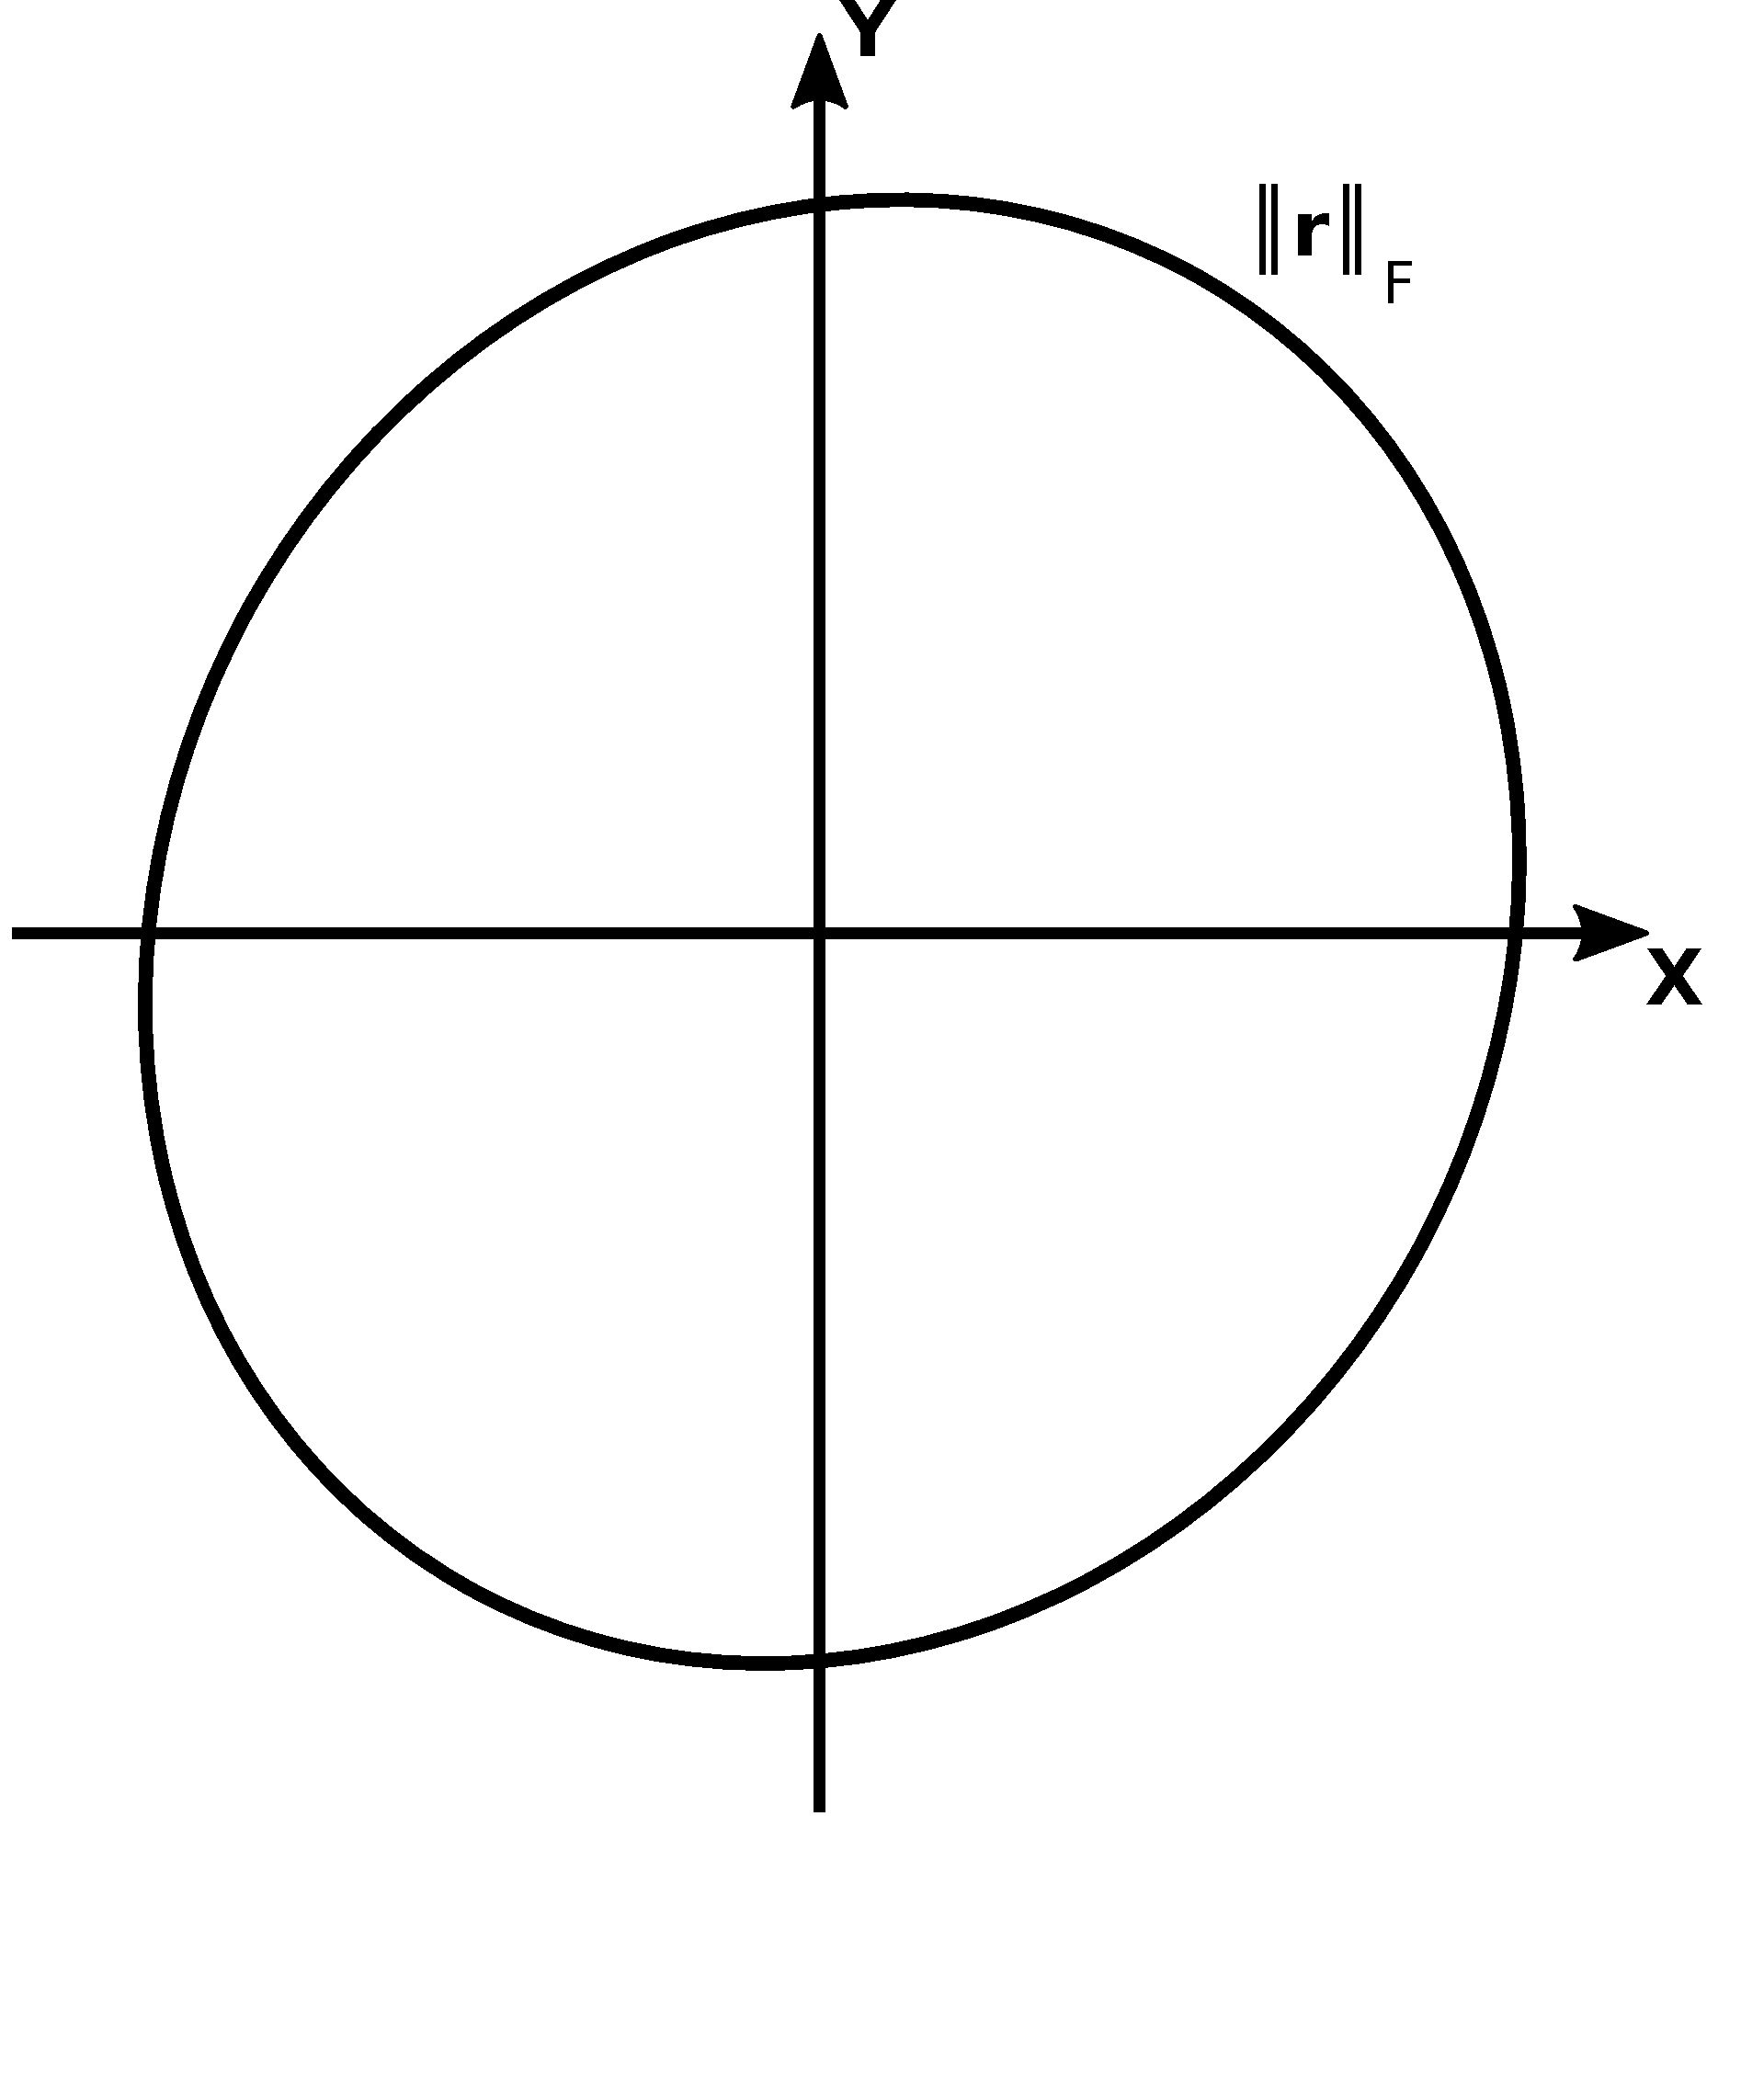
\includegraphics[width=\linewidth]{images/GPR_Mapping_Zero_Mean-1}
			\onslide<2>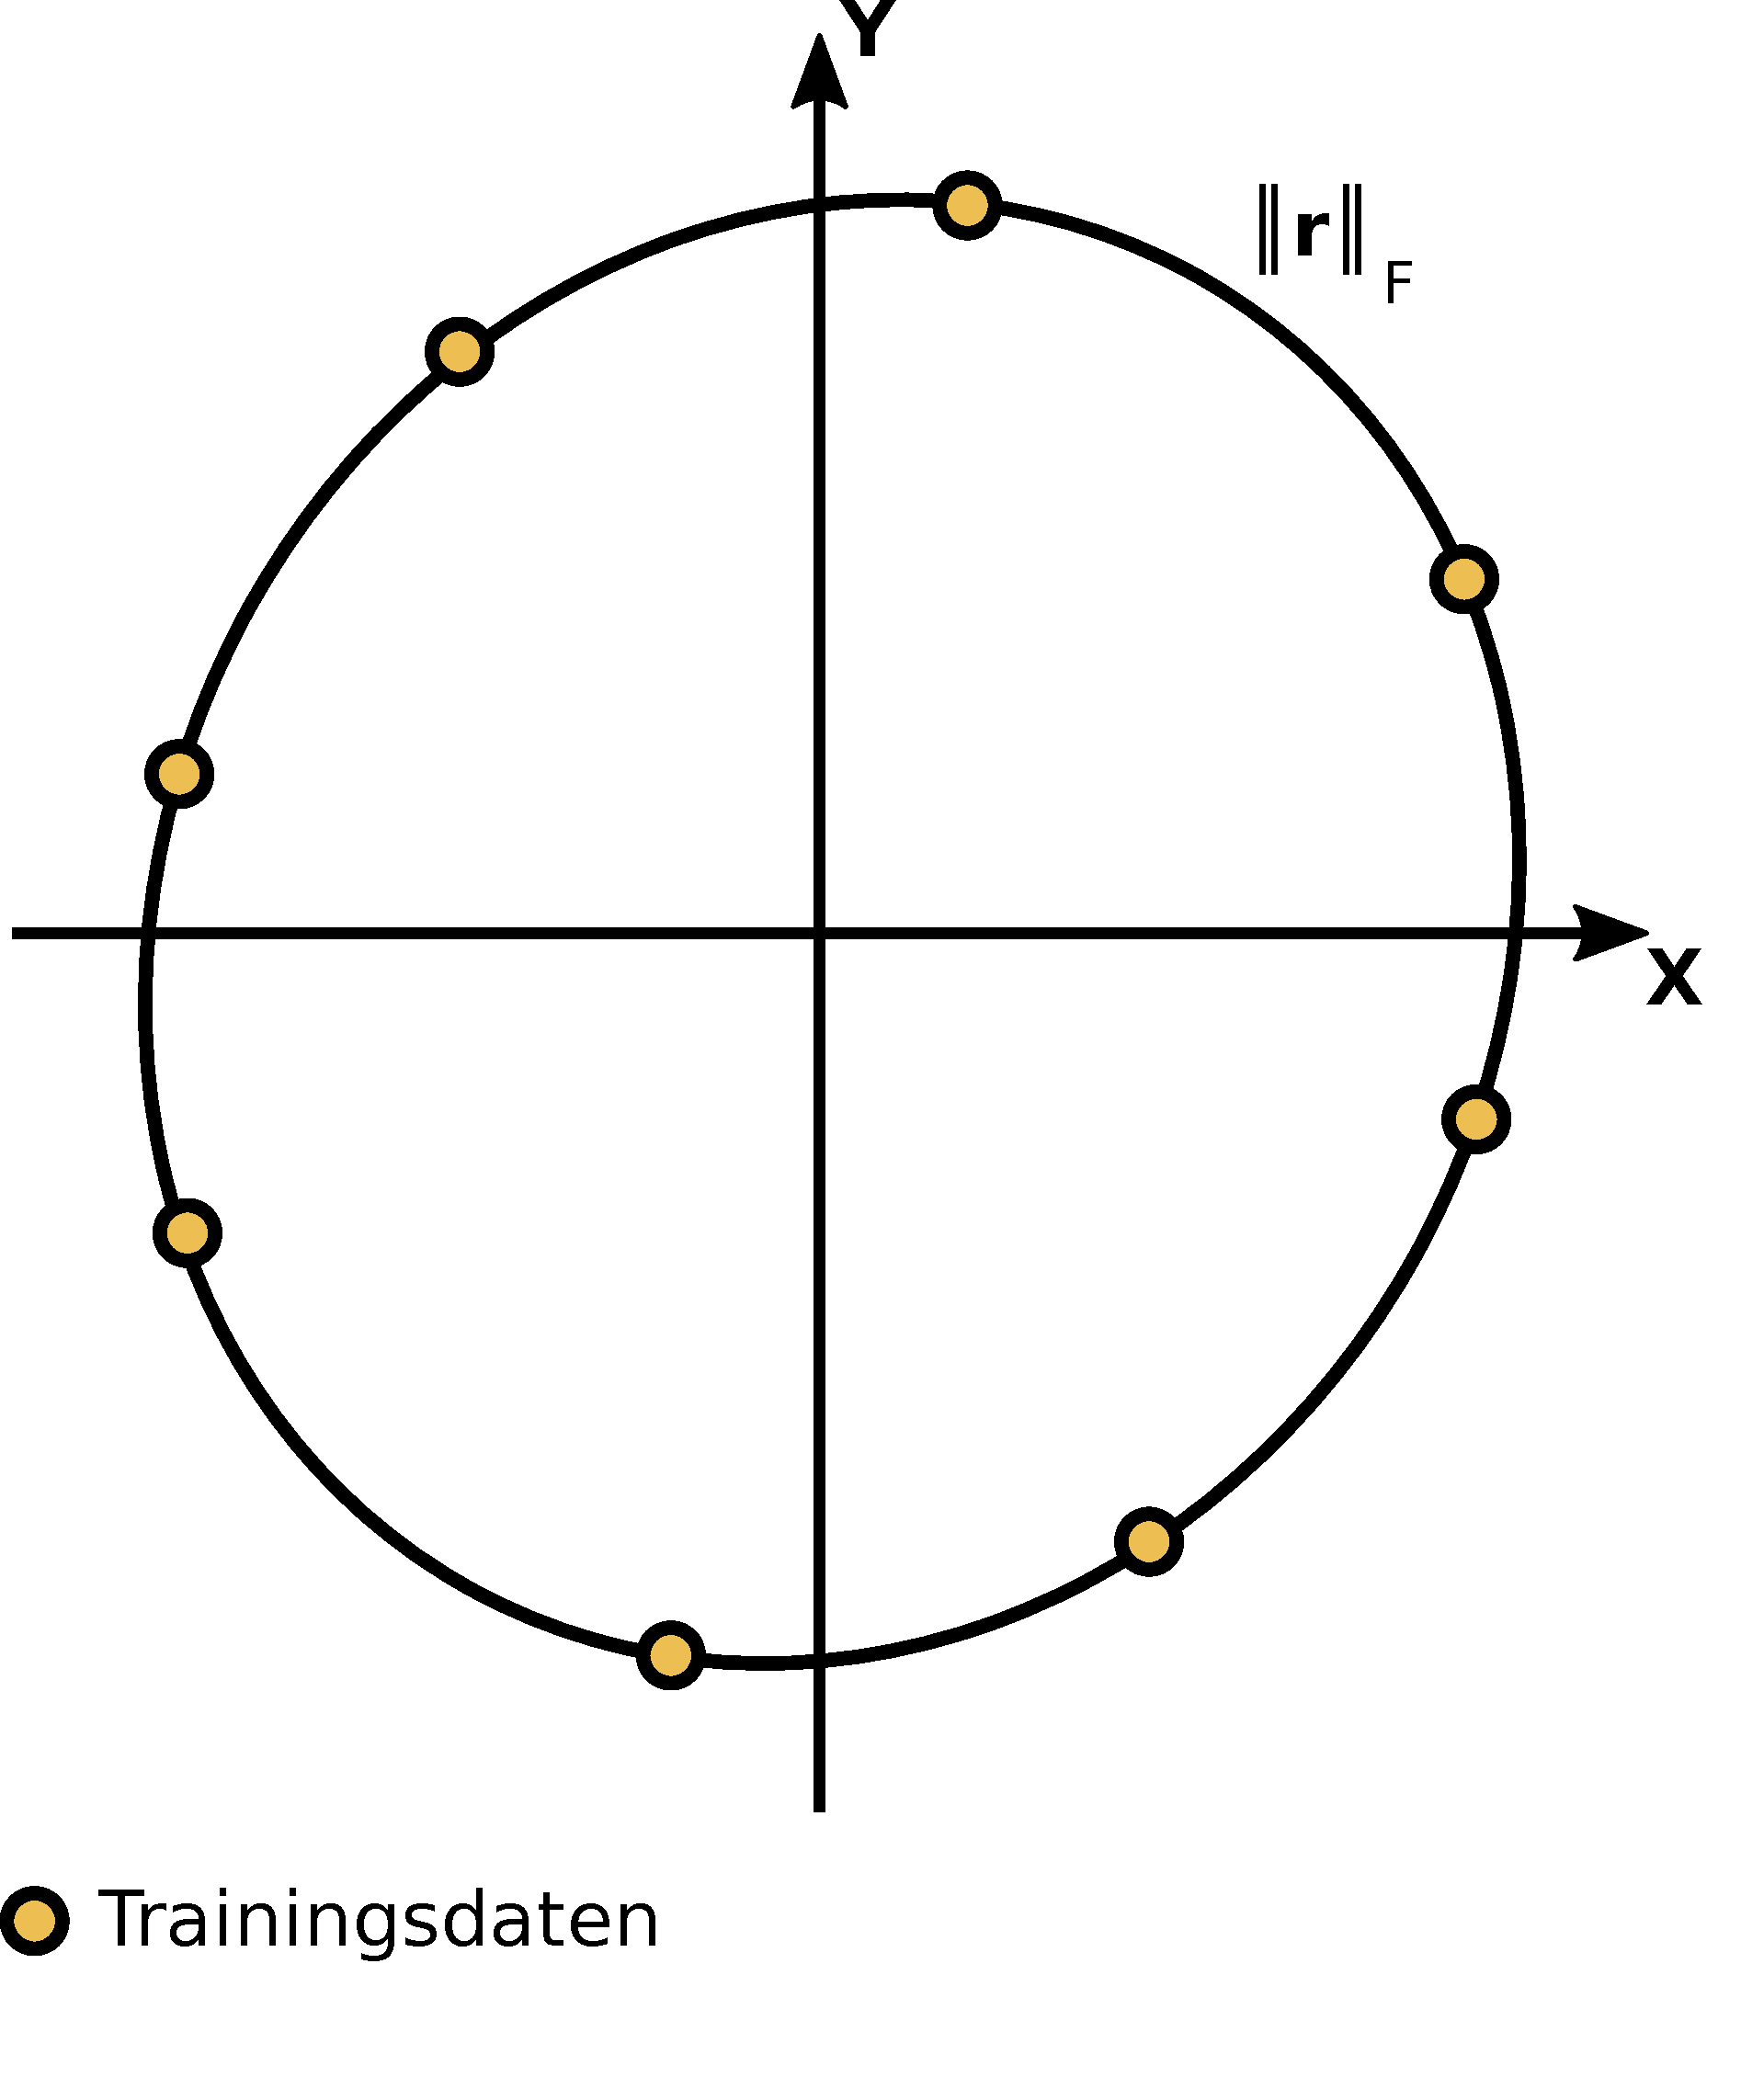
\includegraphics[width=\linewidth]{images/GPR_Mapping_Zero_Mean-2}
			\onslide<3>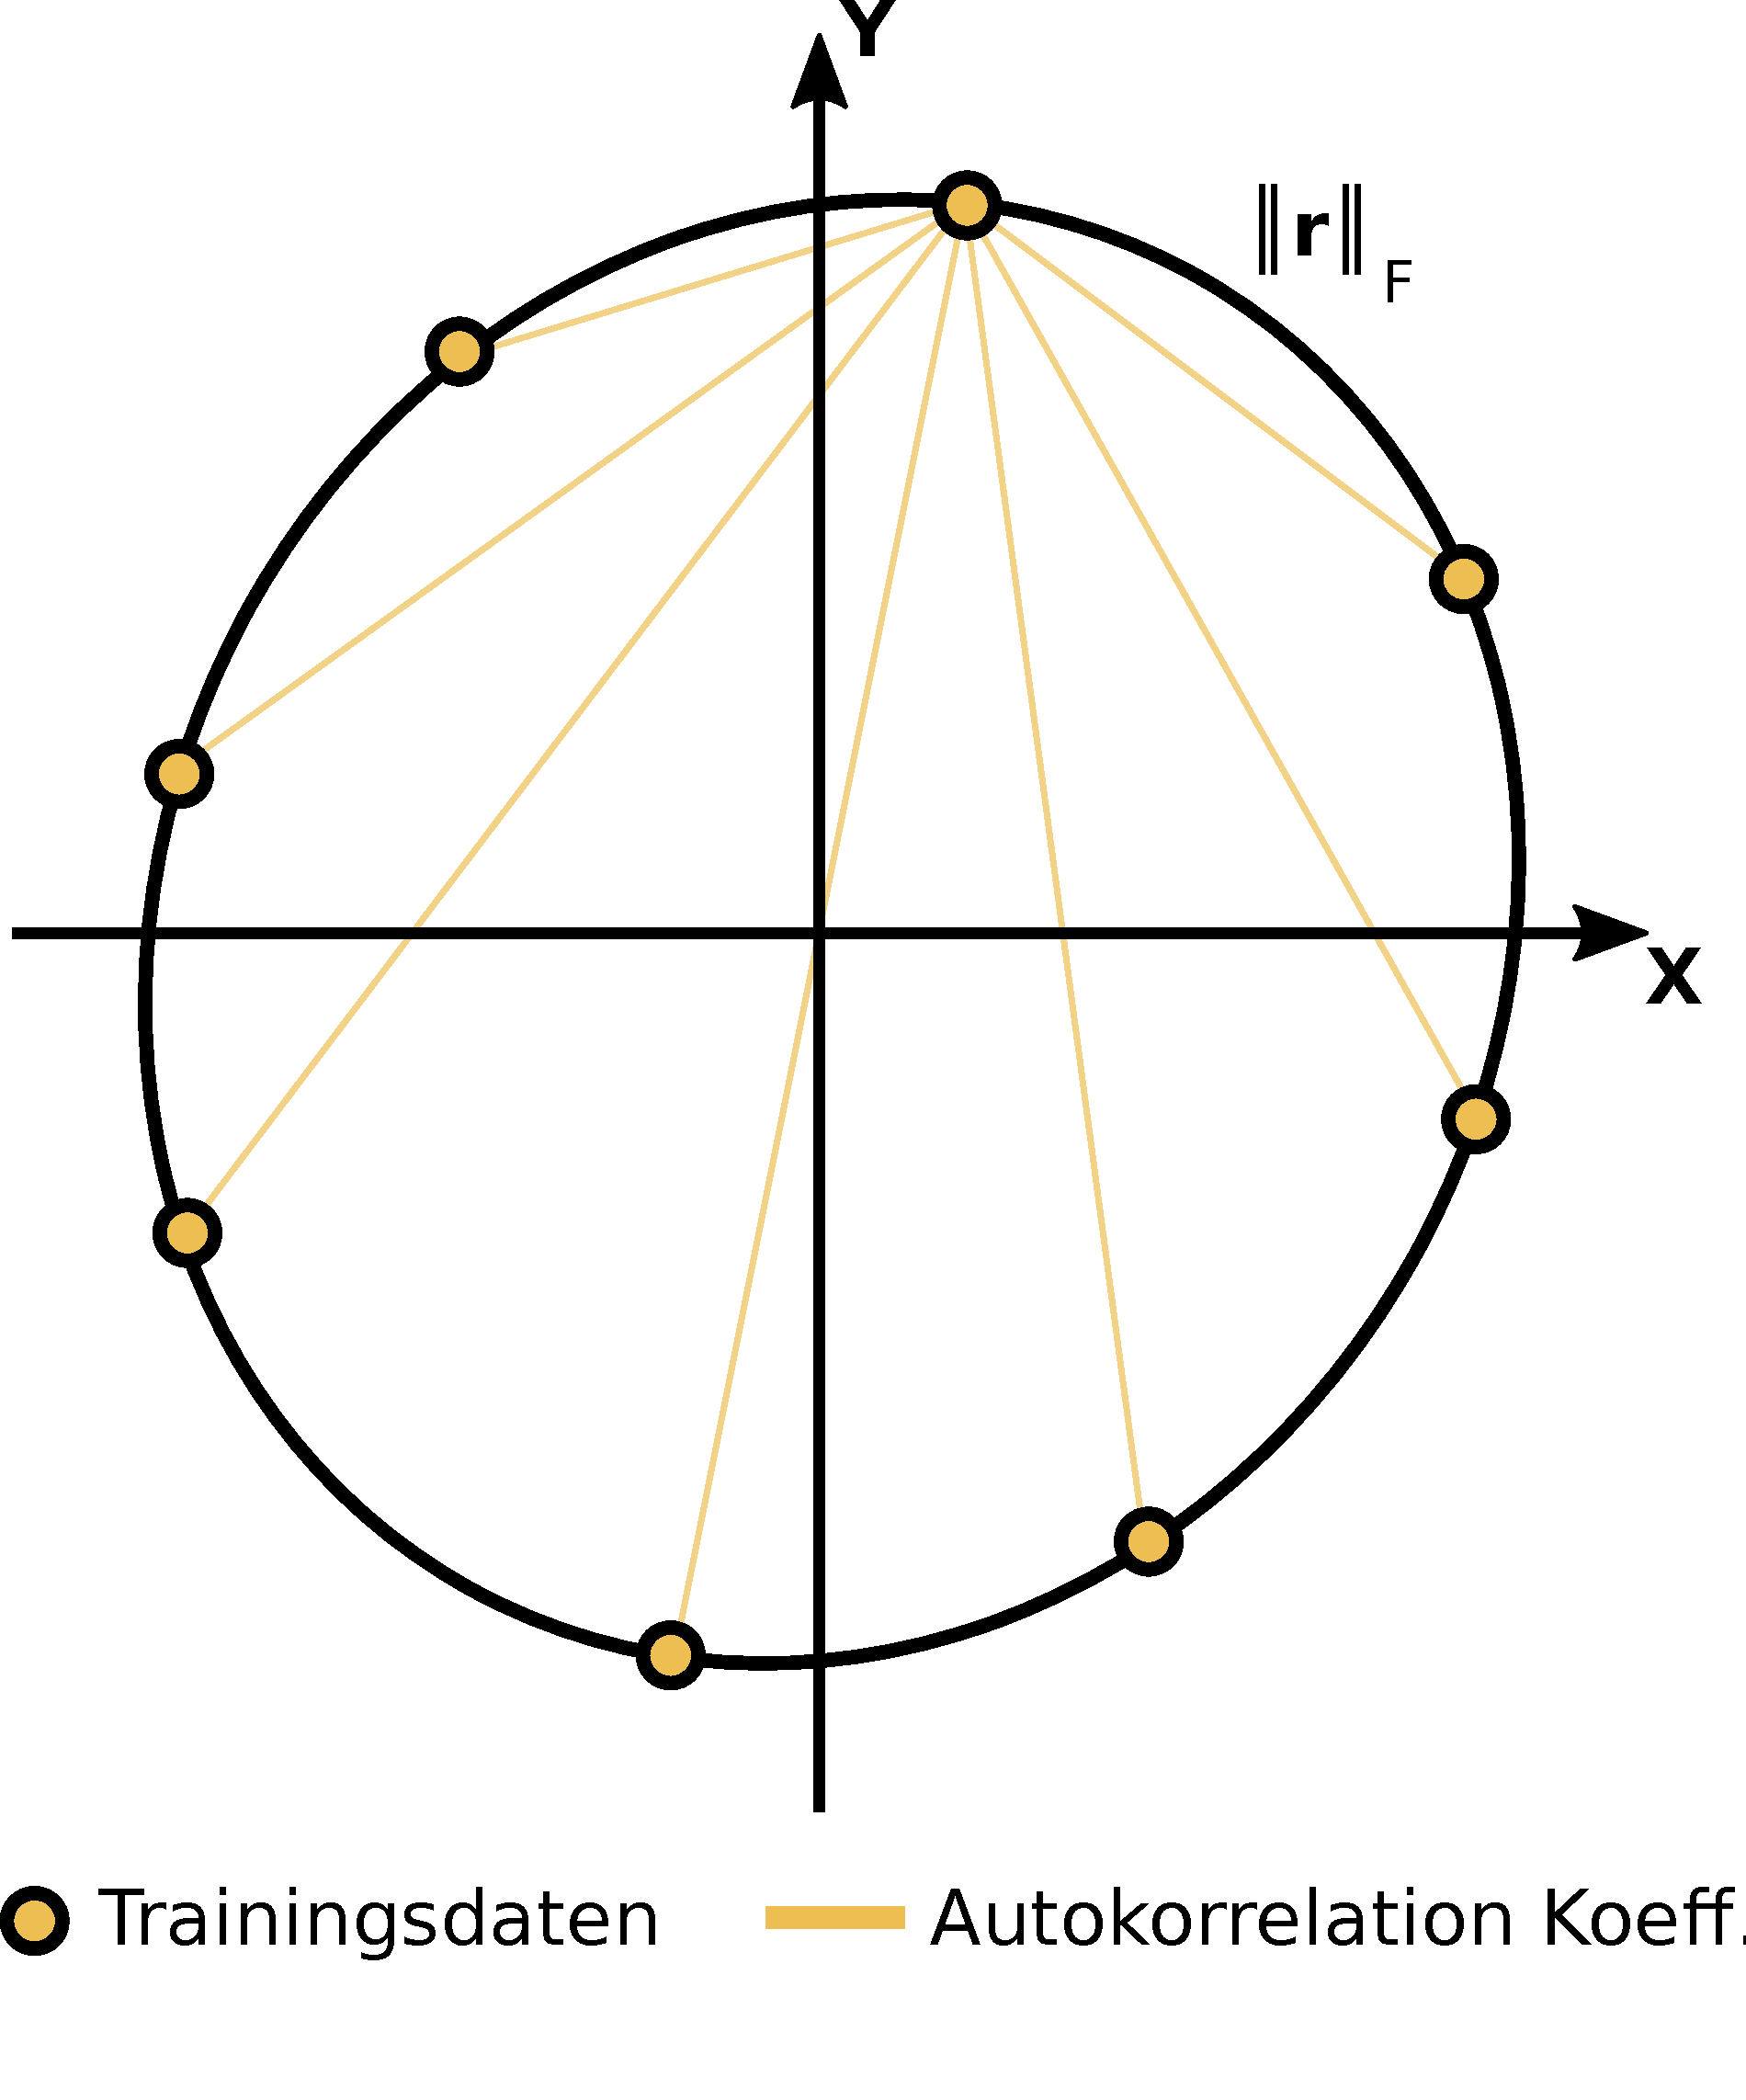
\includegraphics[width=\linewidth]{images/GPR_Mapping_Zero_Mean-3}
			\onslide<4>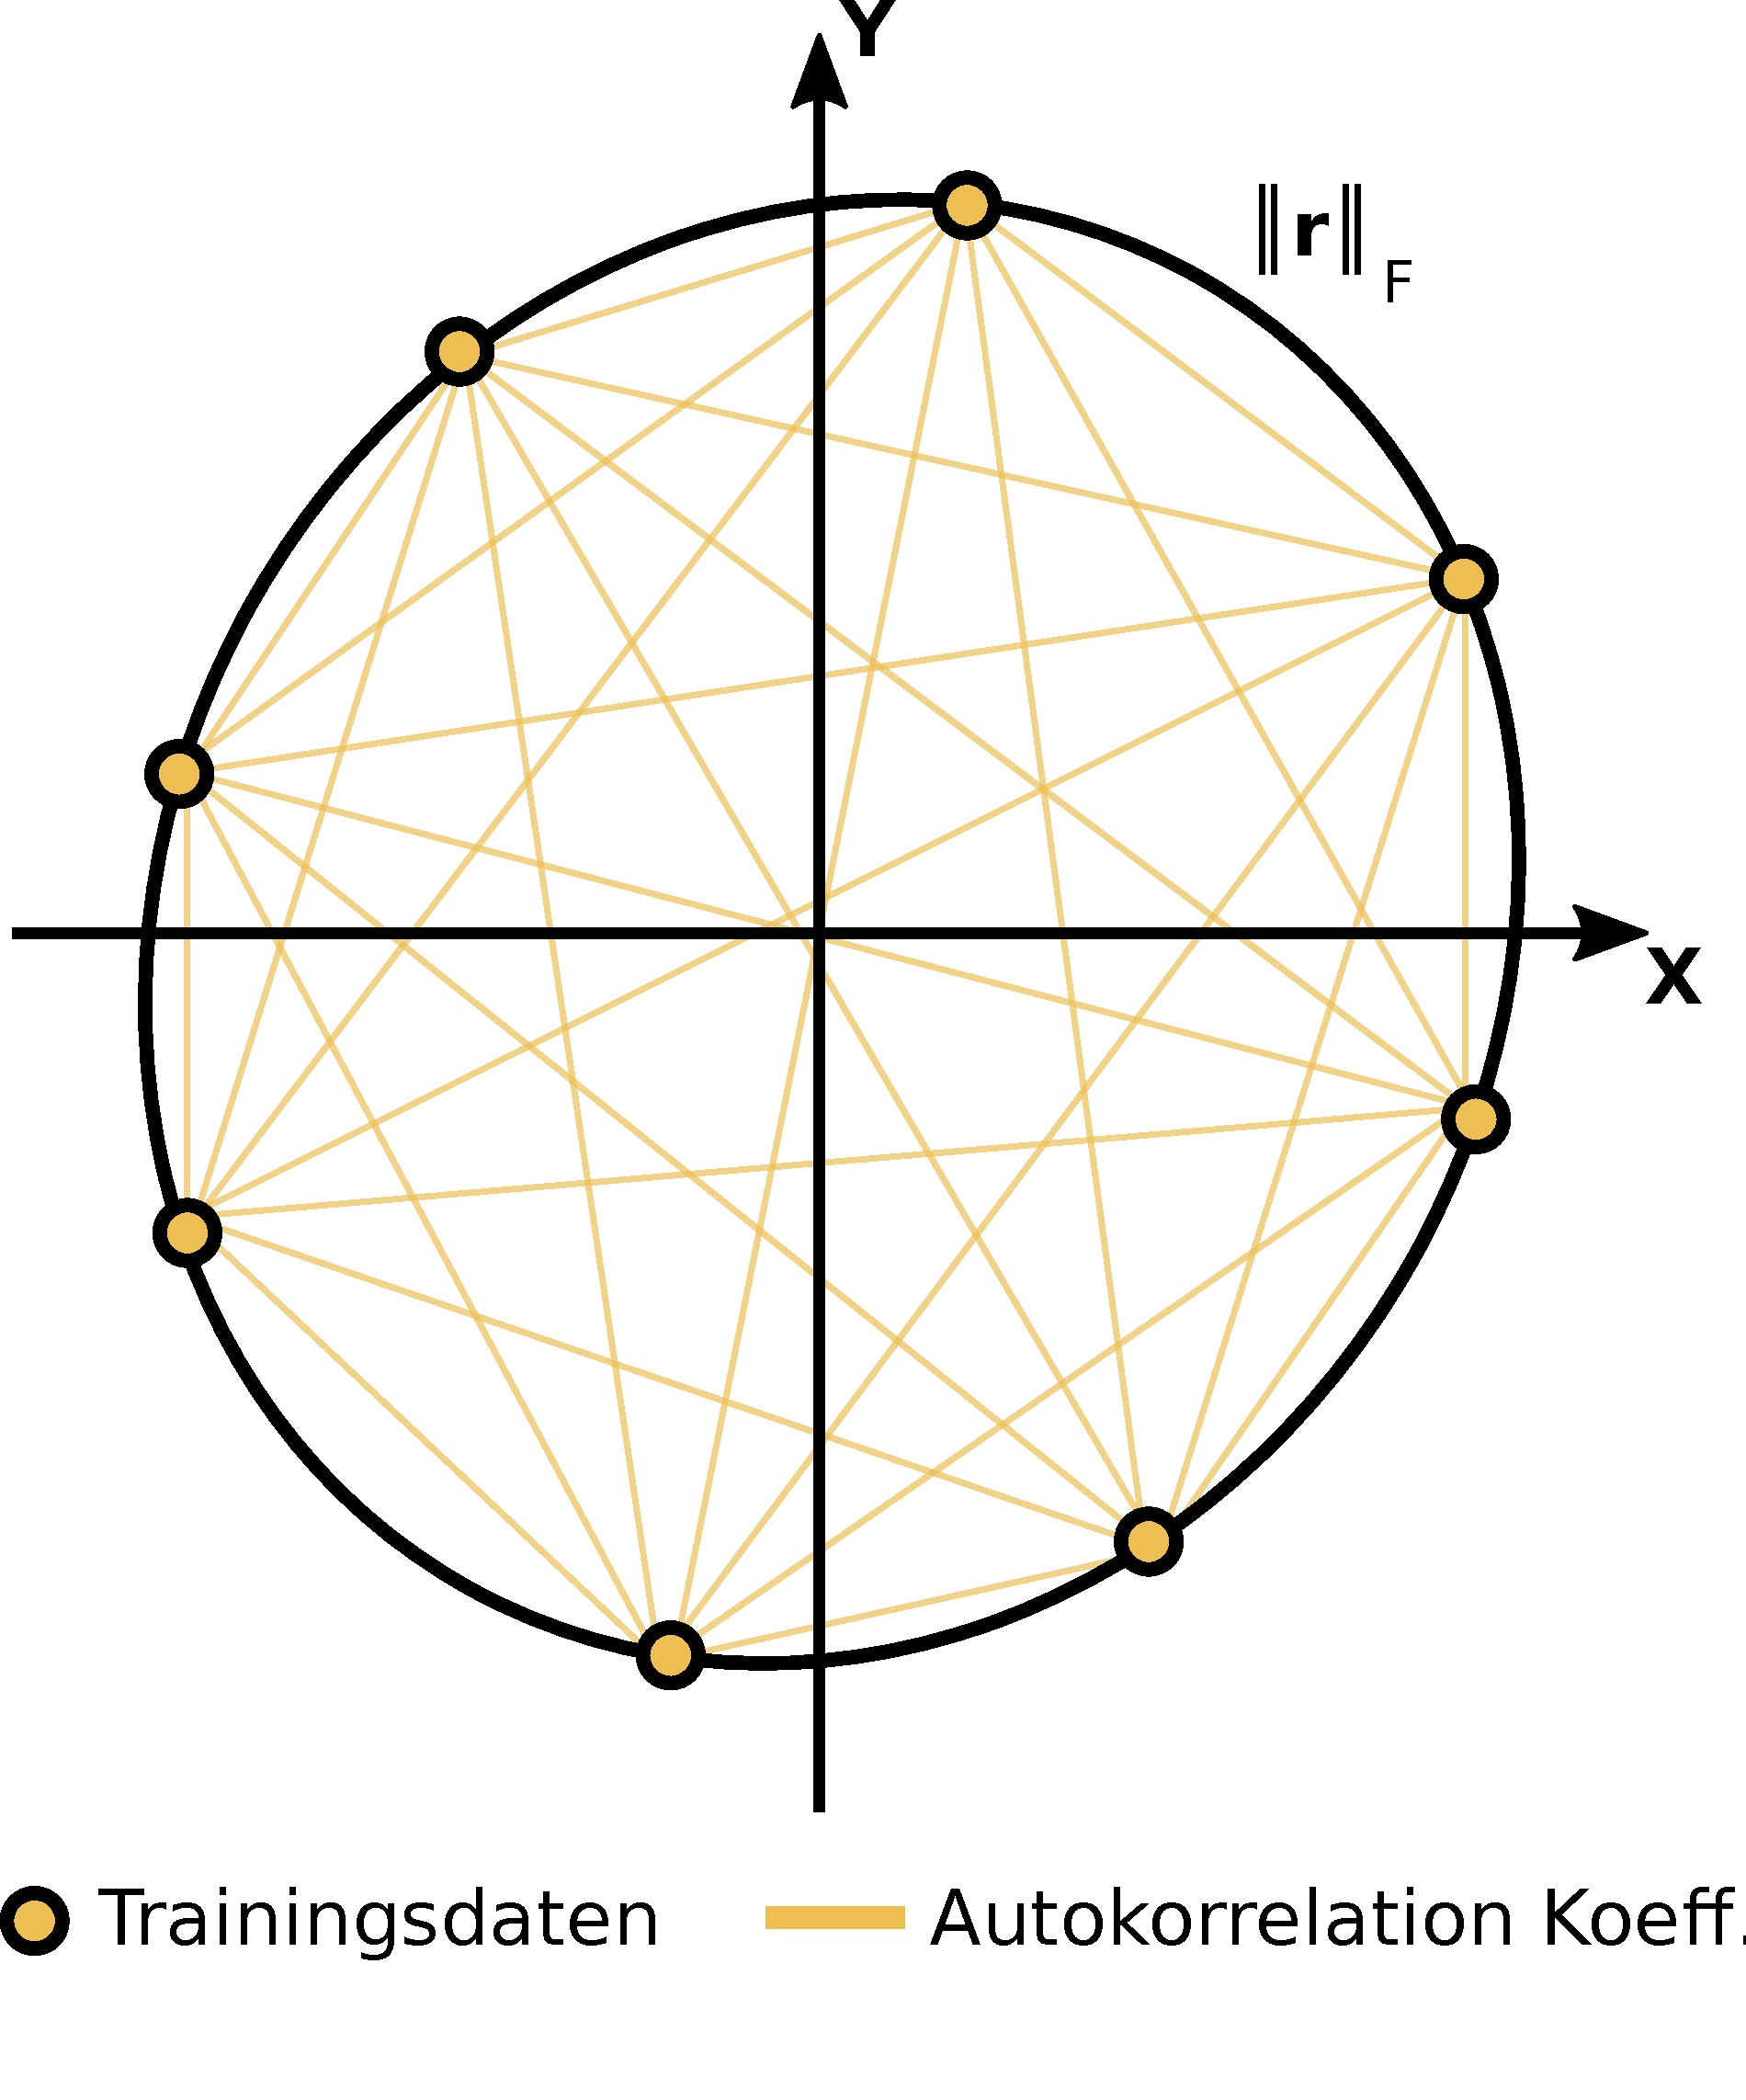
\includegraphics[width=\linewidth]{images/GPR_Mapping_Zero_Mean-4}
			\onslide<5>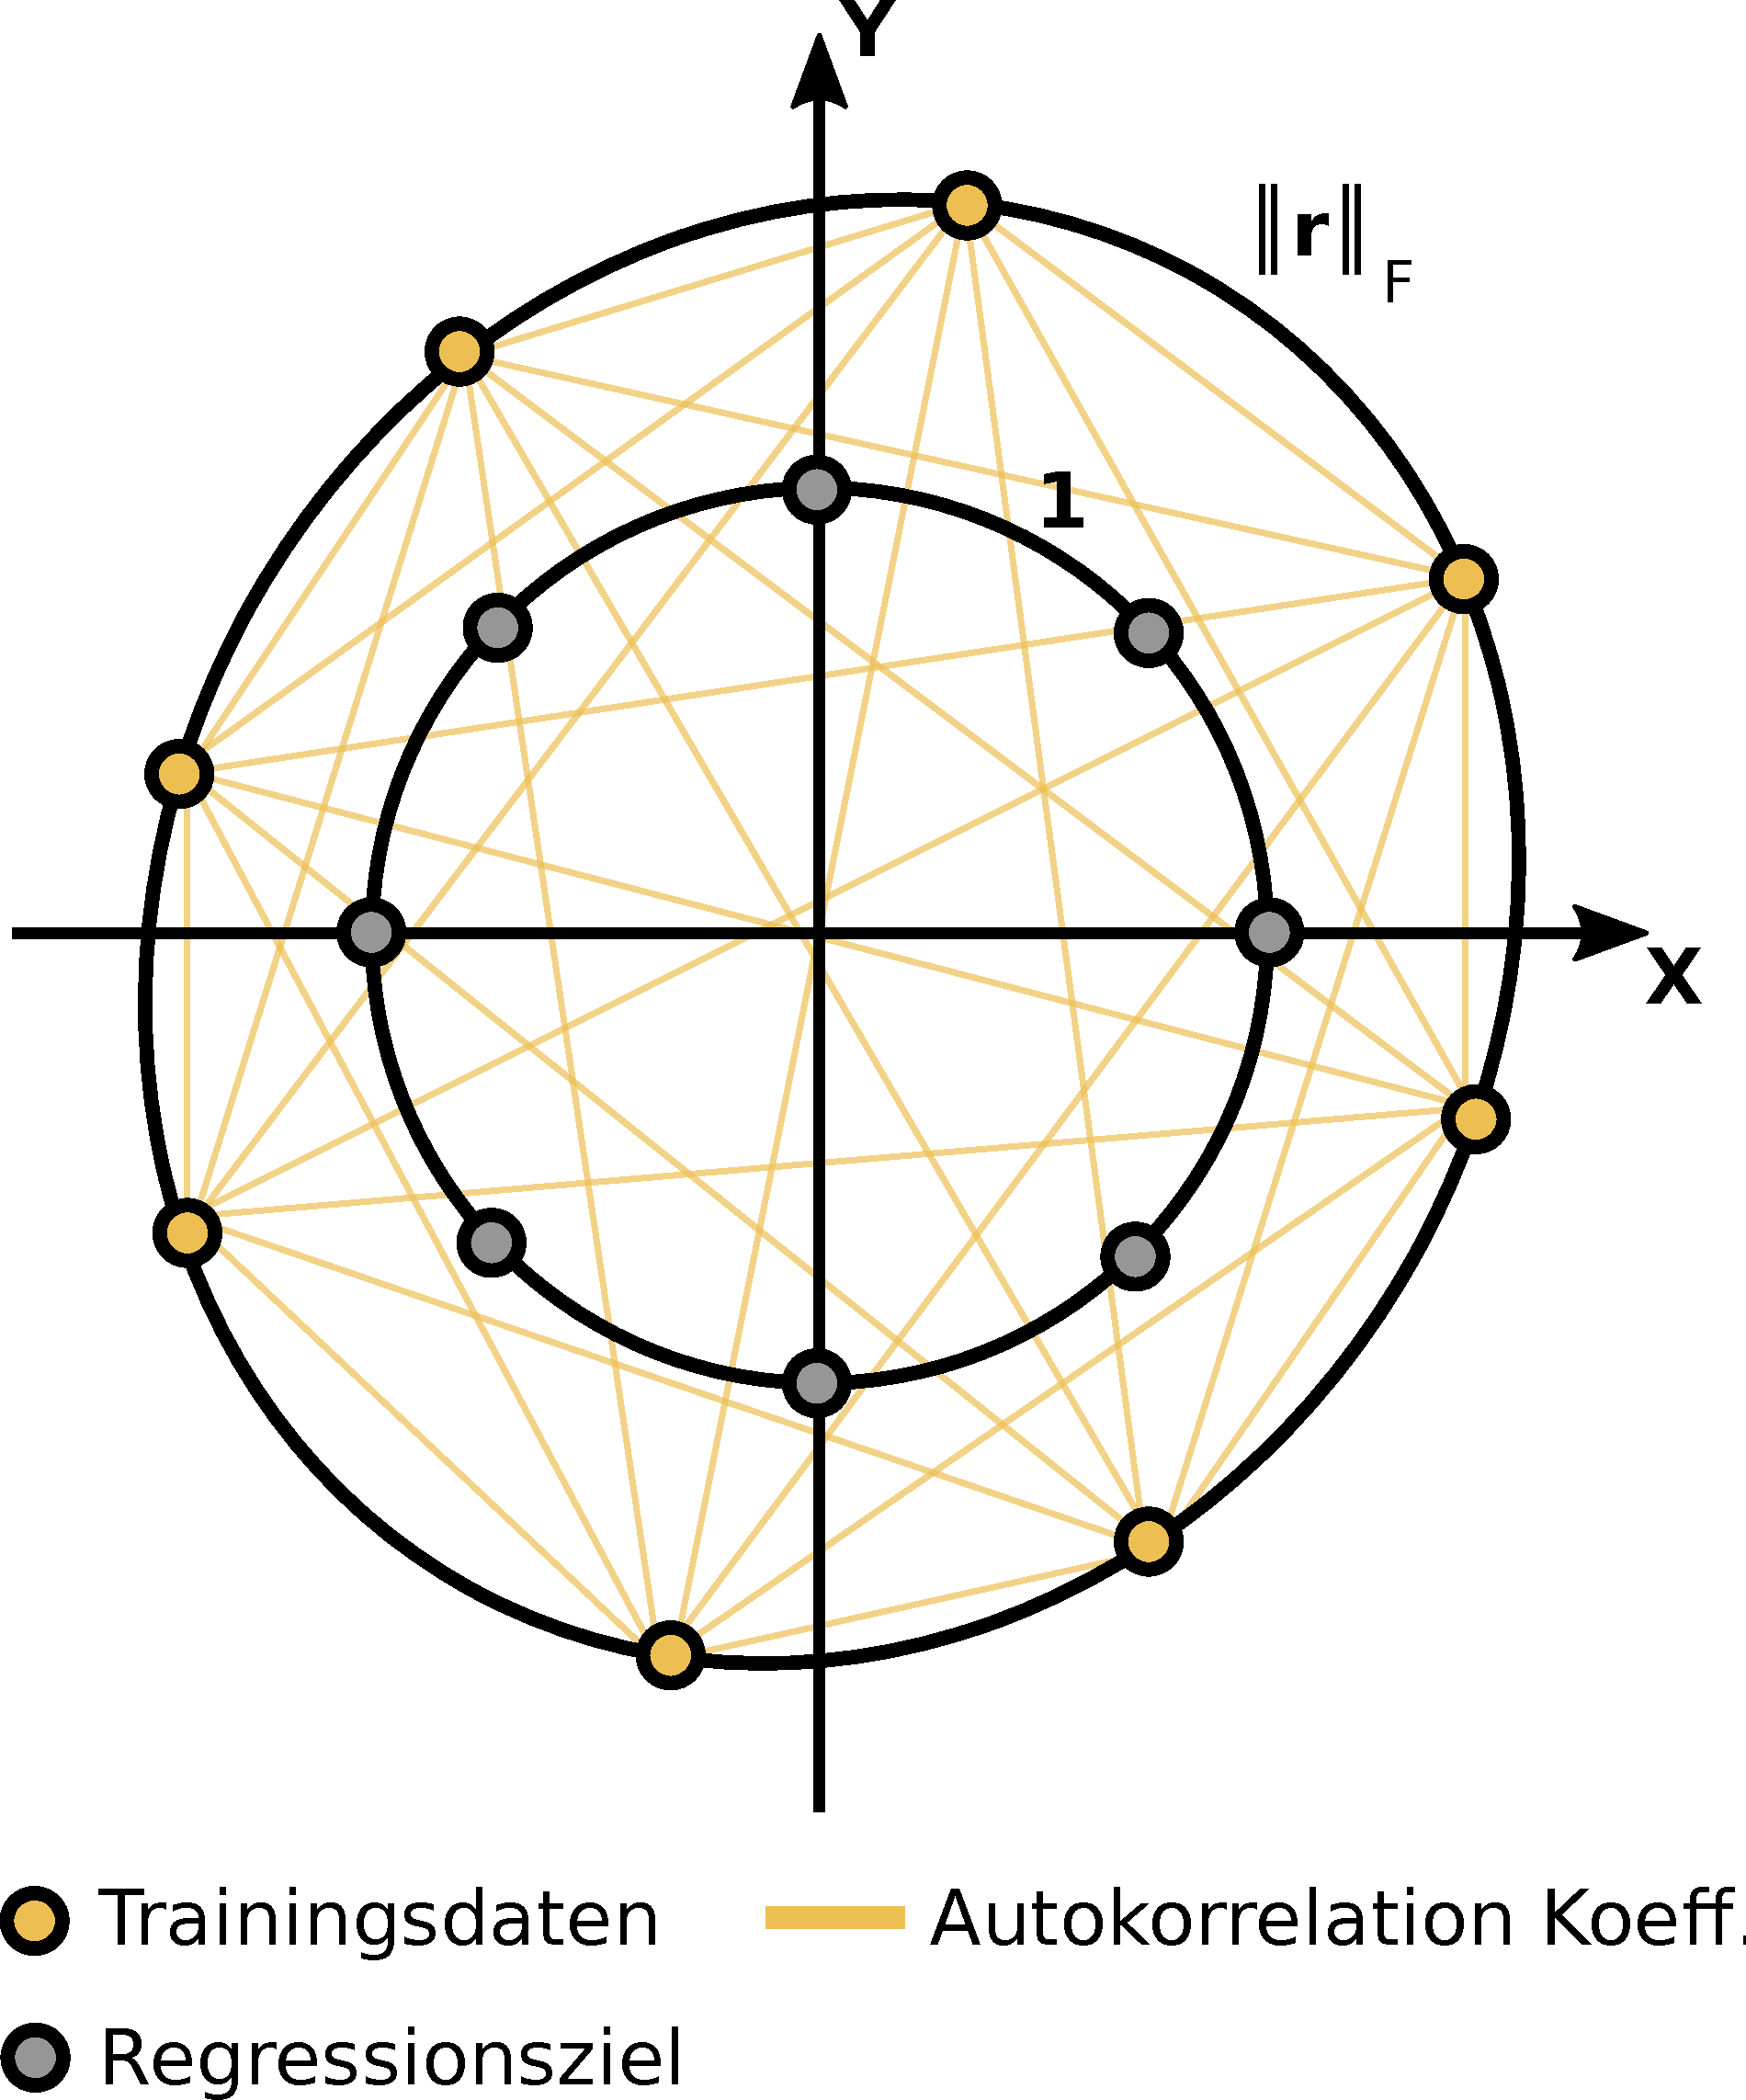
\includegraphics[width=\linewidth]{images/GPR_Mapping_Zero_Mean-5}
			\onslide<6>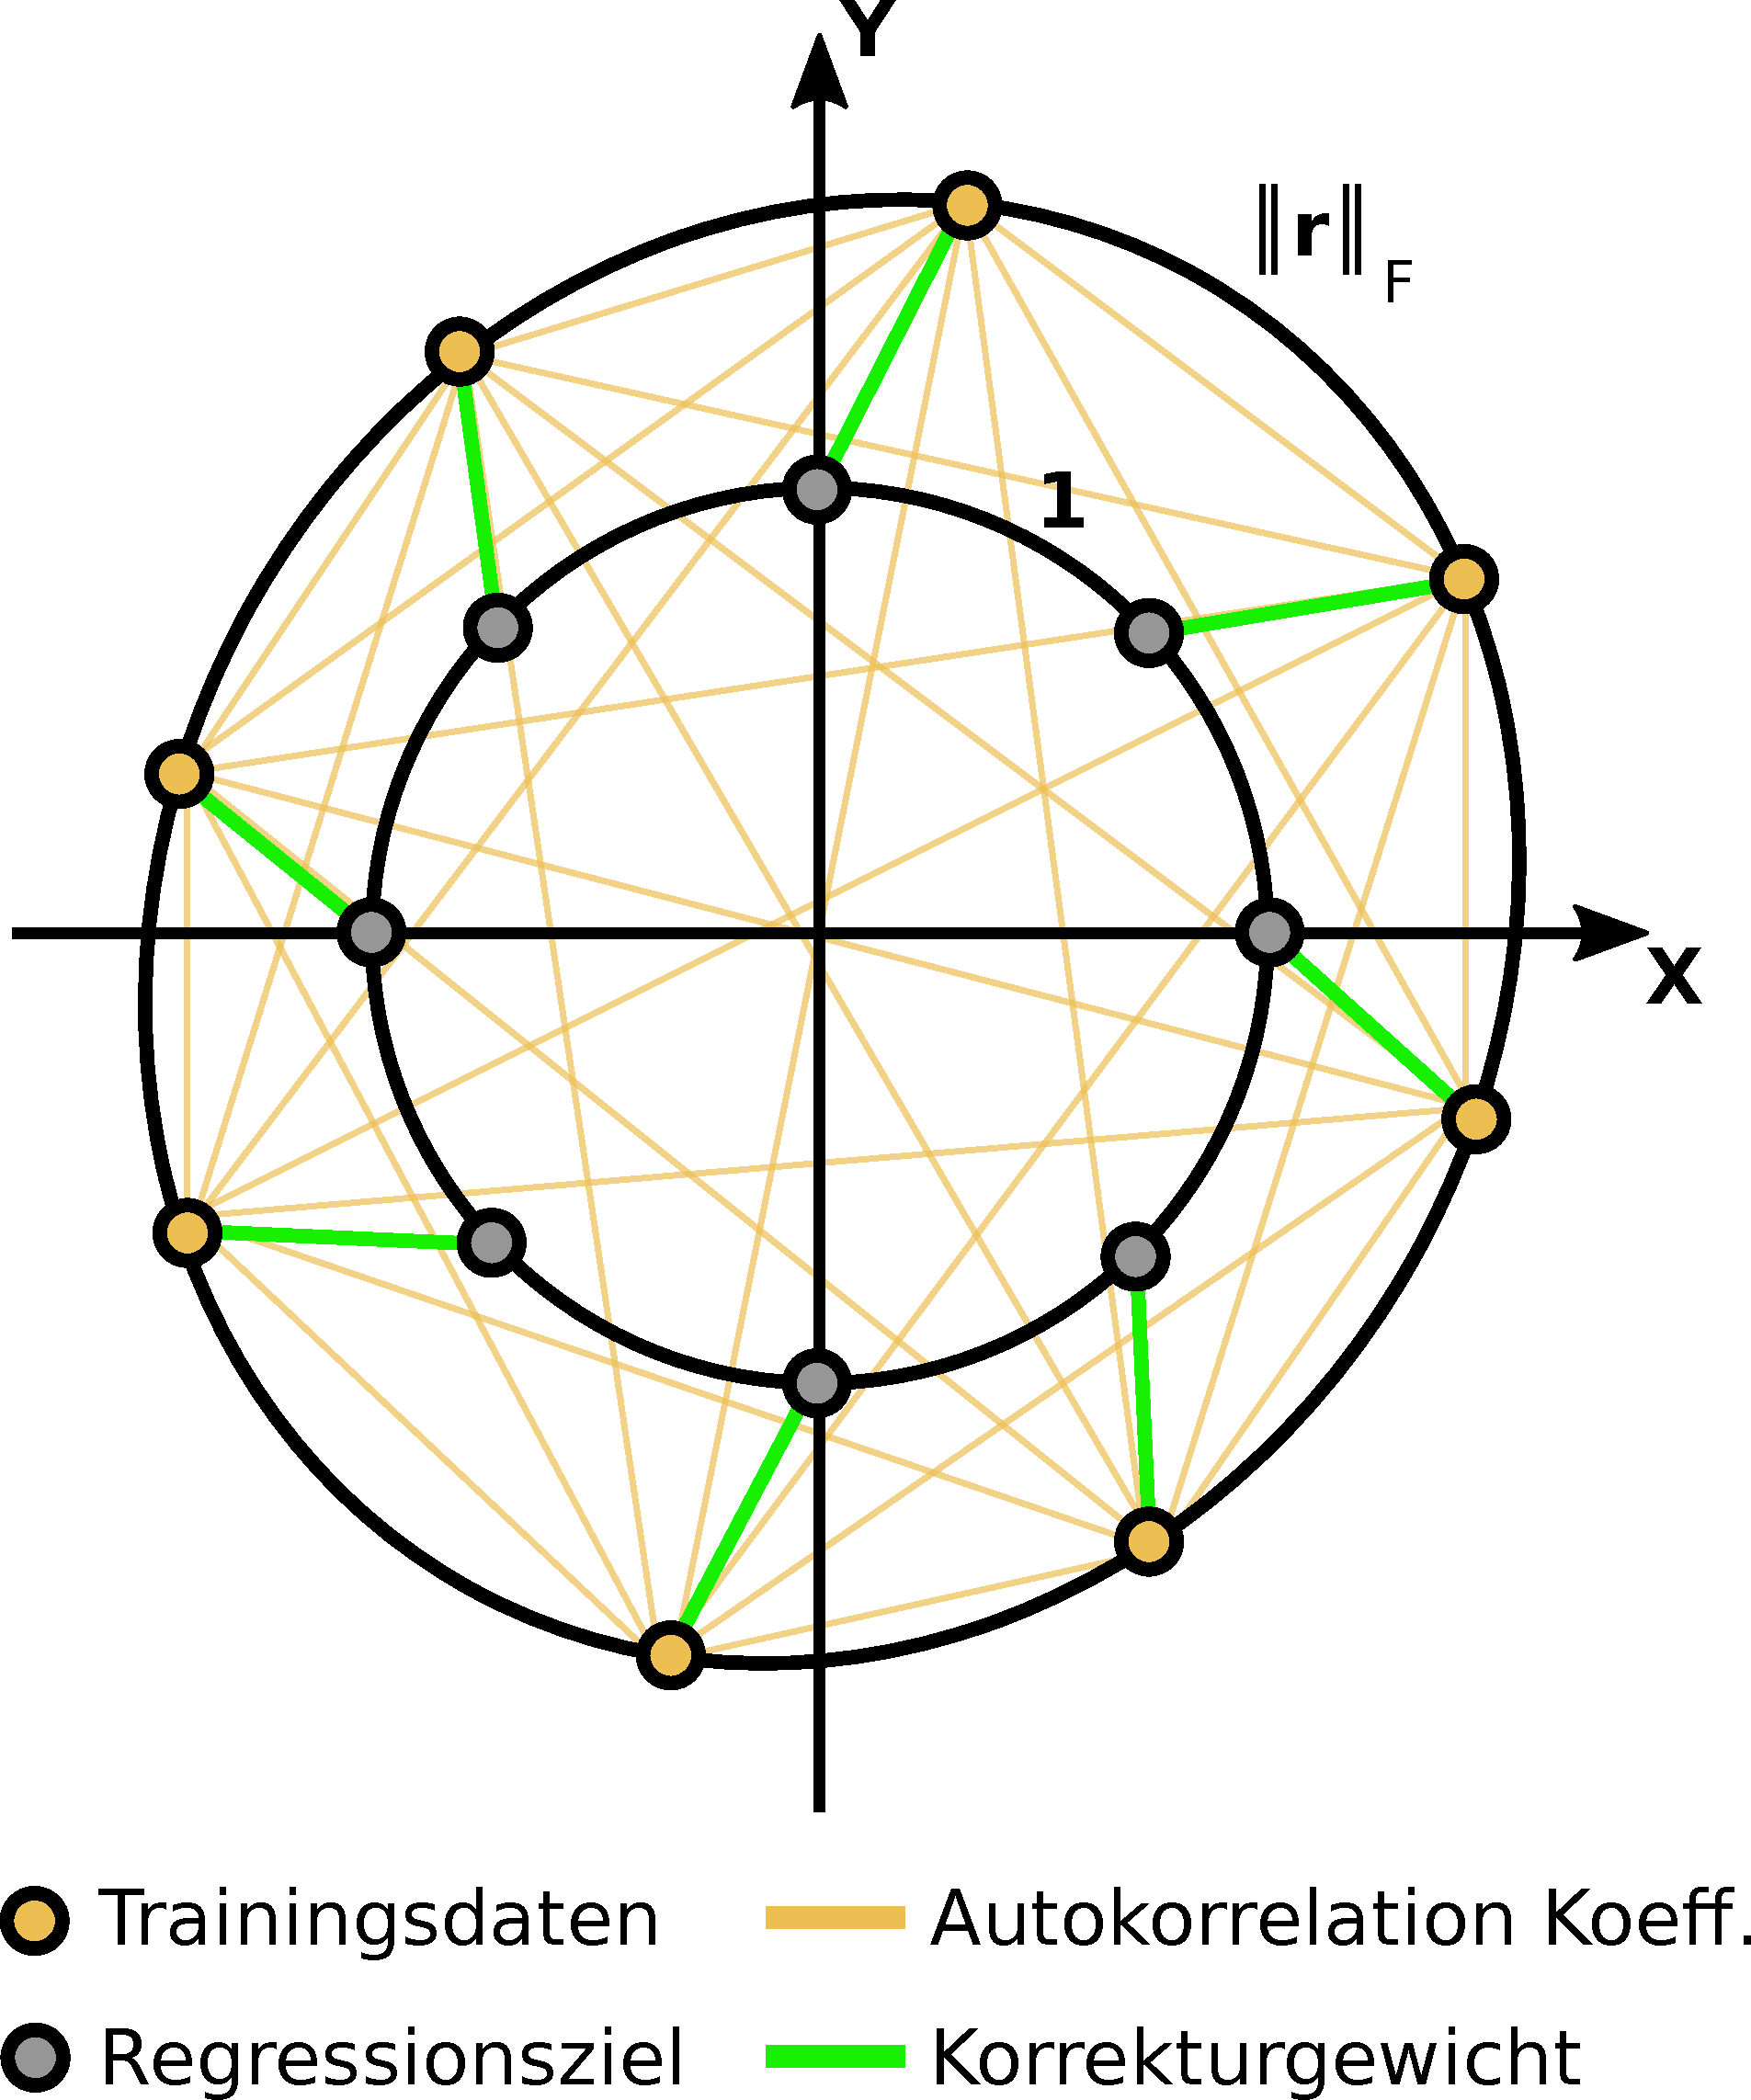
\includegraphics[width=\linewidth]{images/GPR_Mapping_Zero_Mean}
		\end{overprint}
	\end{figure}
\end{columns}
\end{frame}
%%%%%%%%%%%%%%%%%%%%%%%%%%%%%%%%%%%%%%%%%%%%%%%%%%%%%%%%%%%%%%%%%%%%%%%%%%%%%%%%%%%%%%%%%%%%%%%%%%%%%%%%%%%%%%%%%%%%%%%%%%%%%%%%%%%%%%%%%
\subsection{Kreisdarstellung - GPR mit Mittelwertkorrektur}
\begin{frame}
\frametitle{GPR-Verfahren}
\framesubtitle{Kreisdarstellung - GPR mit Mittelwertkorrektur}
\begin{columns}[c]
	\column{.5\textwidth}
	\begin{itemize}
		\item<1-> Trainingsdaten, Autokorrelation identisch
		\item<2-> Mittelwertbildung üb. $m(X)=H'(X) \cdot \beta$
		\item<3-> 2. Gewichtsniveau durch Mittelwert
		\item<3-> Vorwiegend Amplituden-/ Offset-Korrektur
		\item<4-> Guter Mittelwert, kleine Korrekturgewichte
		\item<4-> Höherer Rechenaufwand
	\end{itemize}
	\column{.45\textwidth}
	\begin{figure}
		\begin{overprint}
			\onslide<1>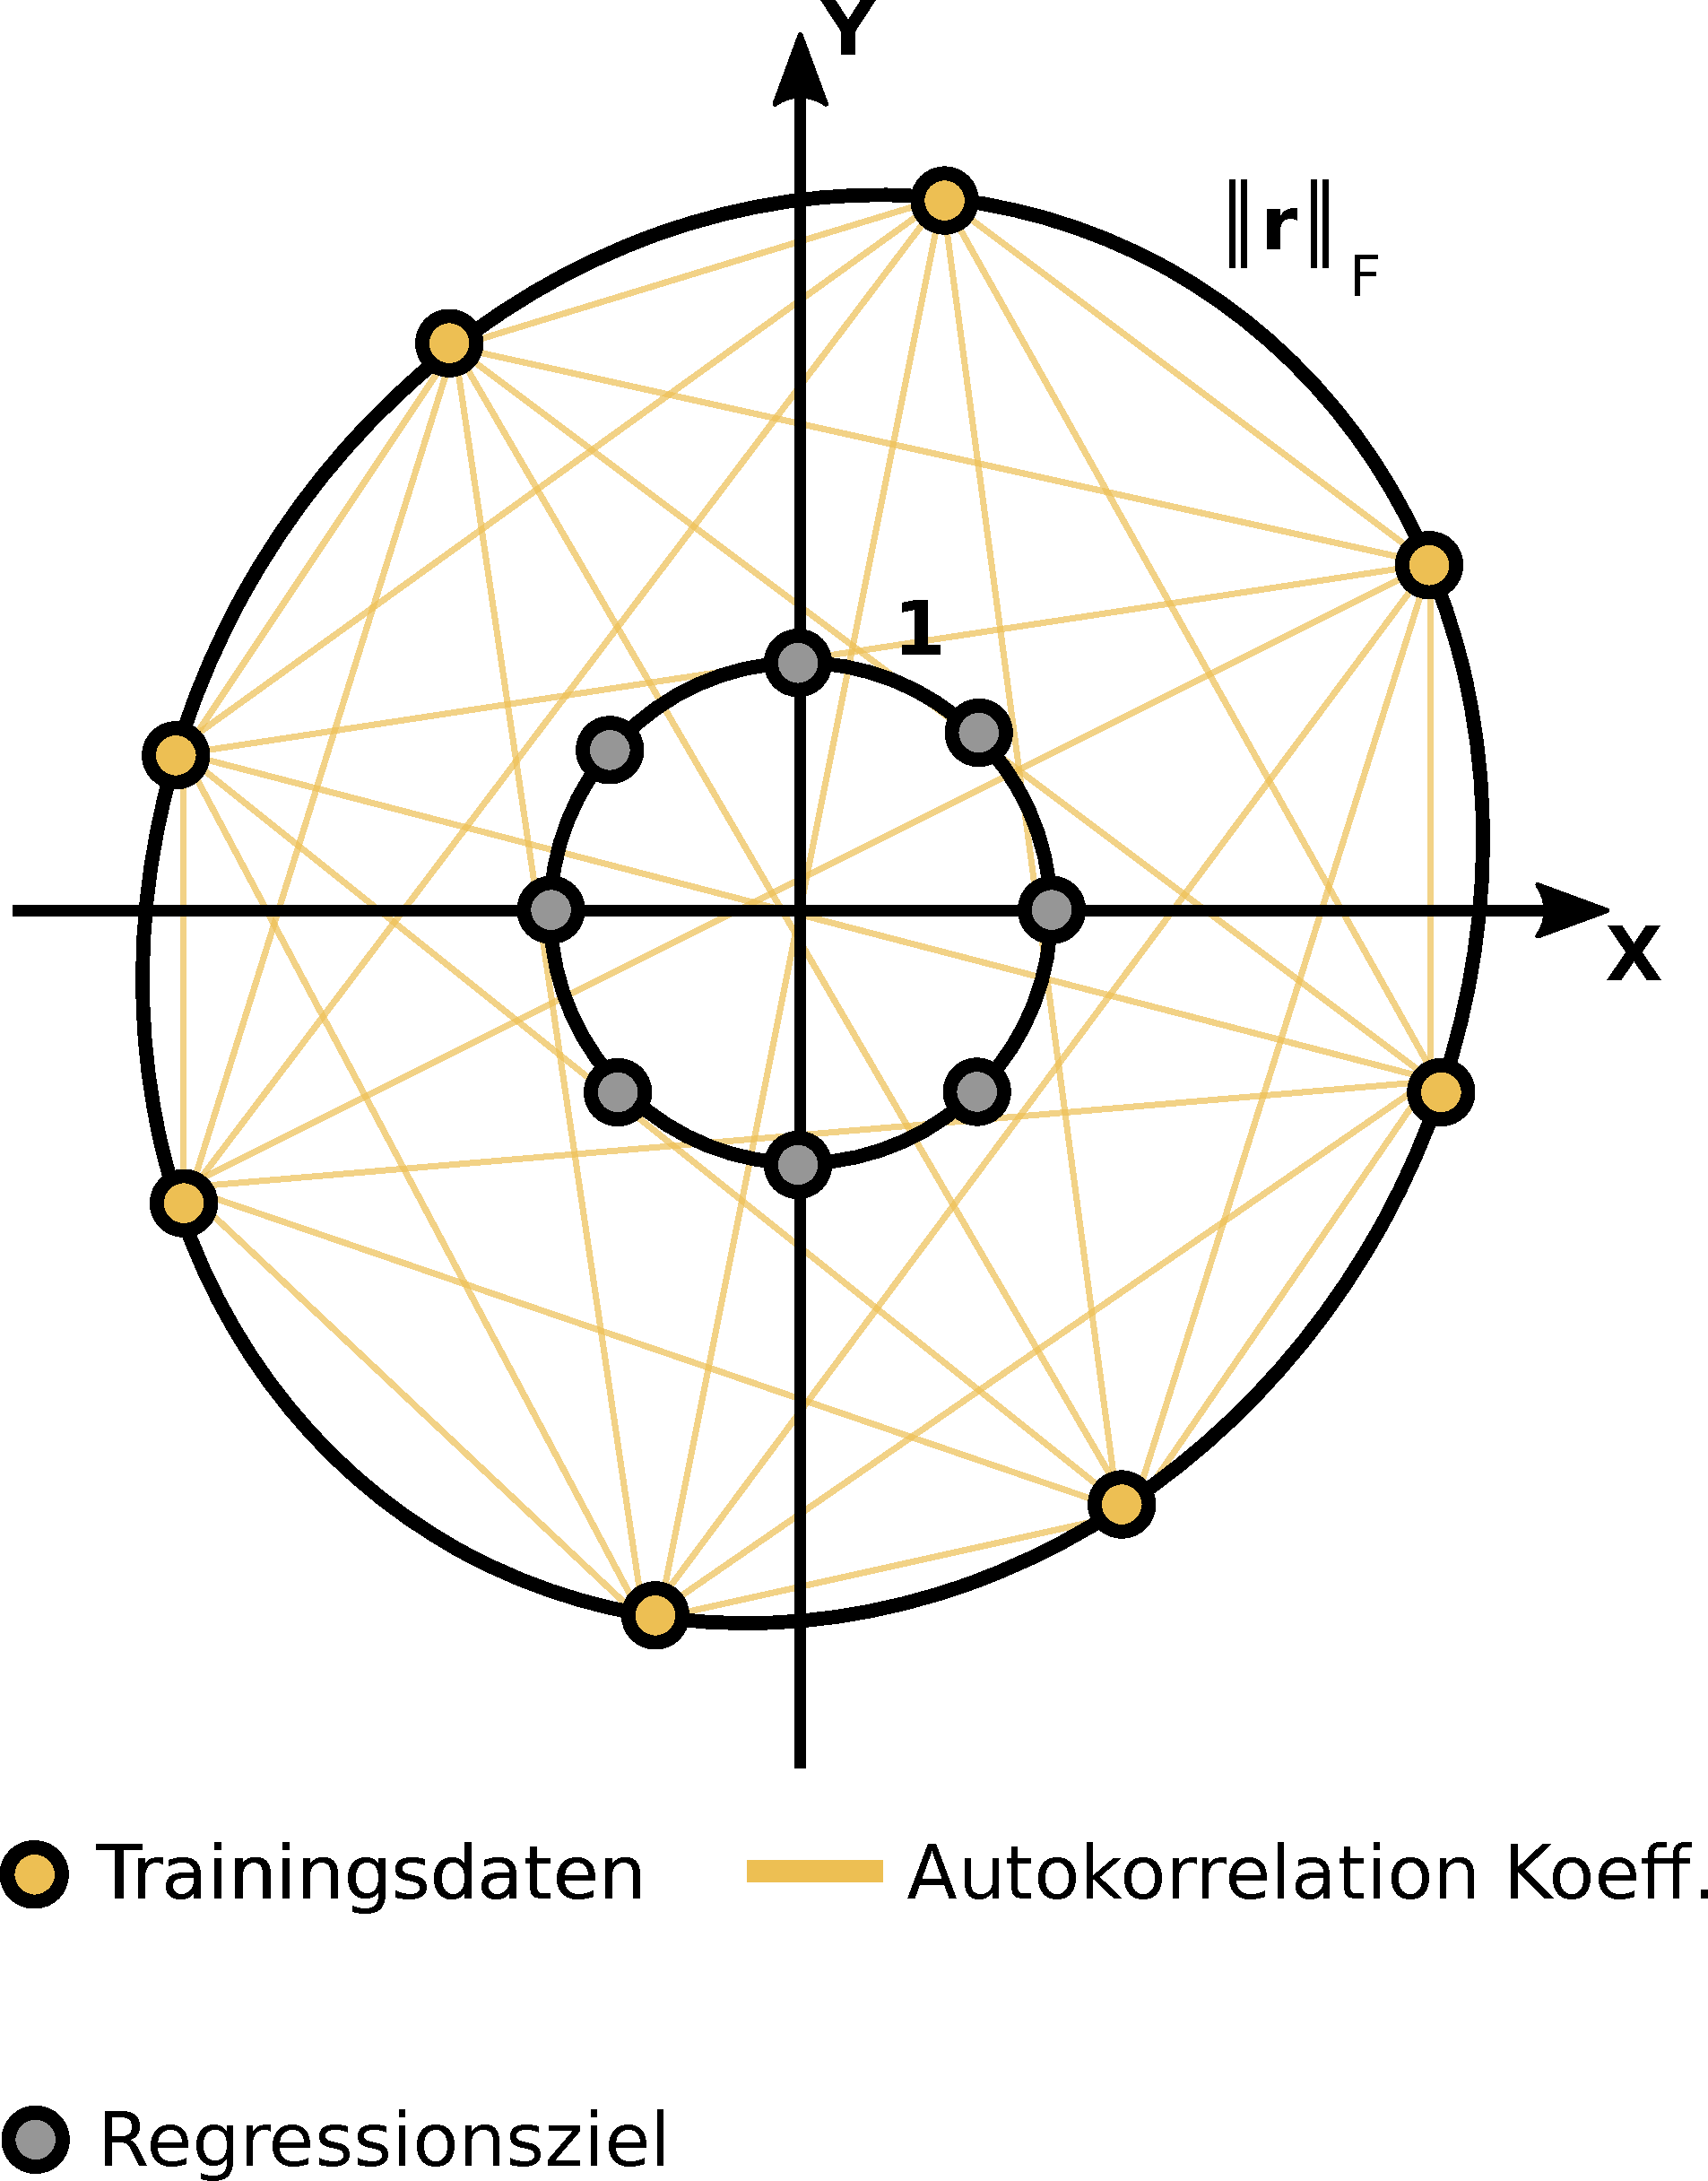
\includegraphics[width=\linewidth]{images/GPR_Mapping_Mean-1}
			\onslide<2>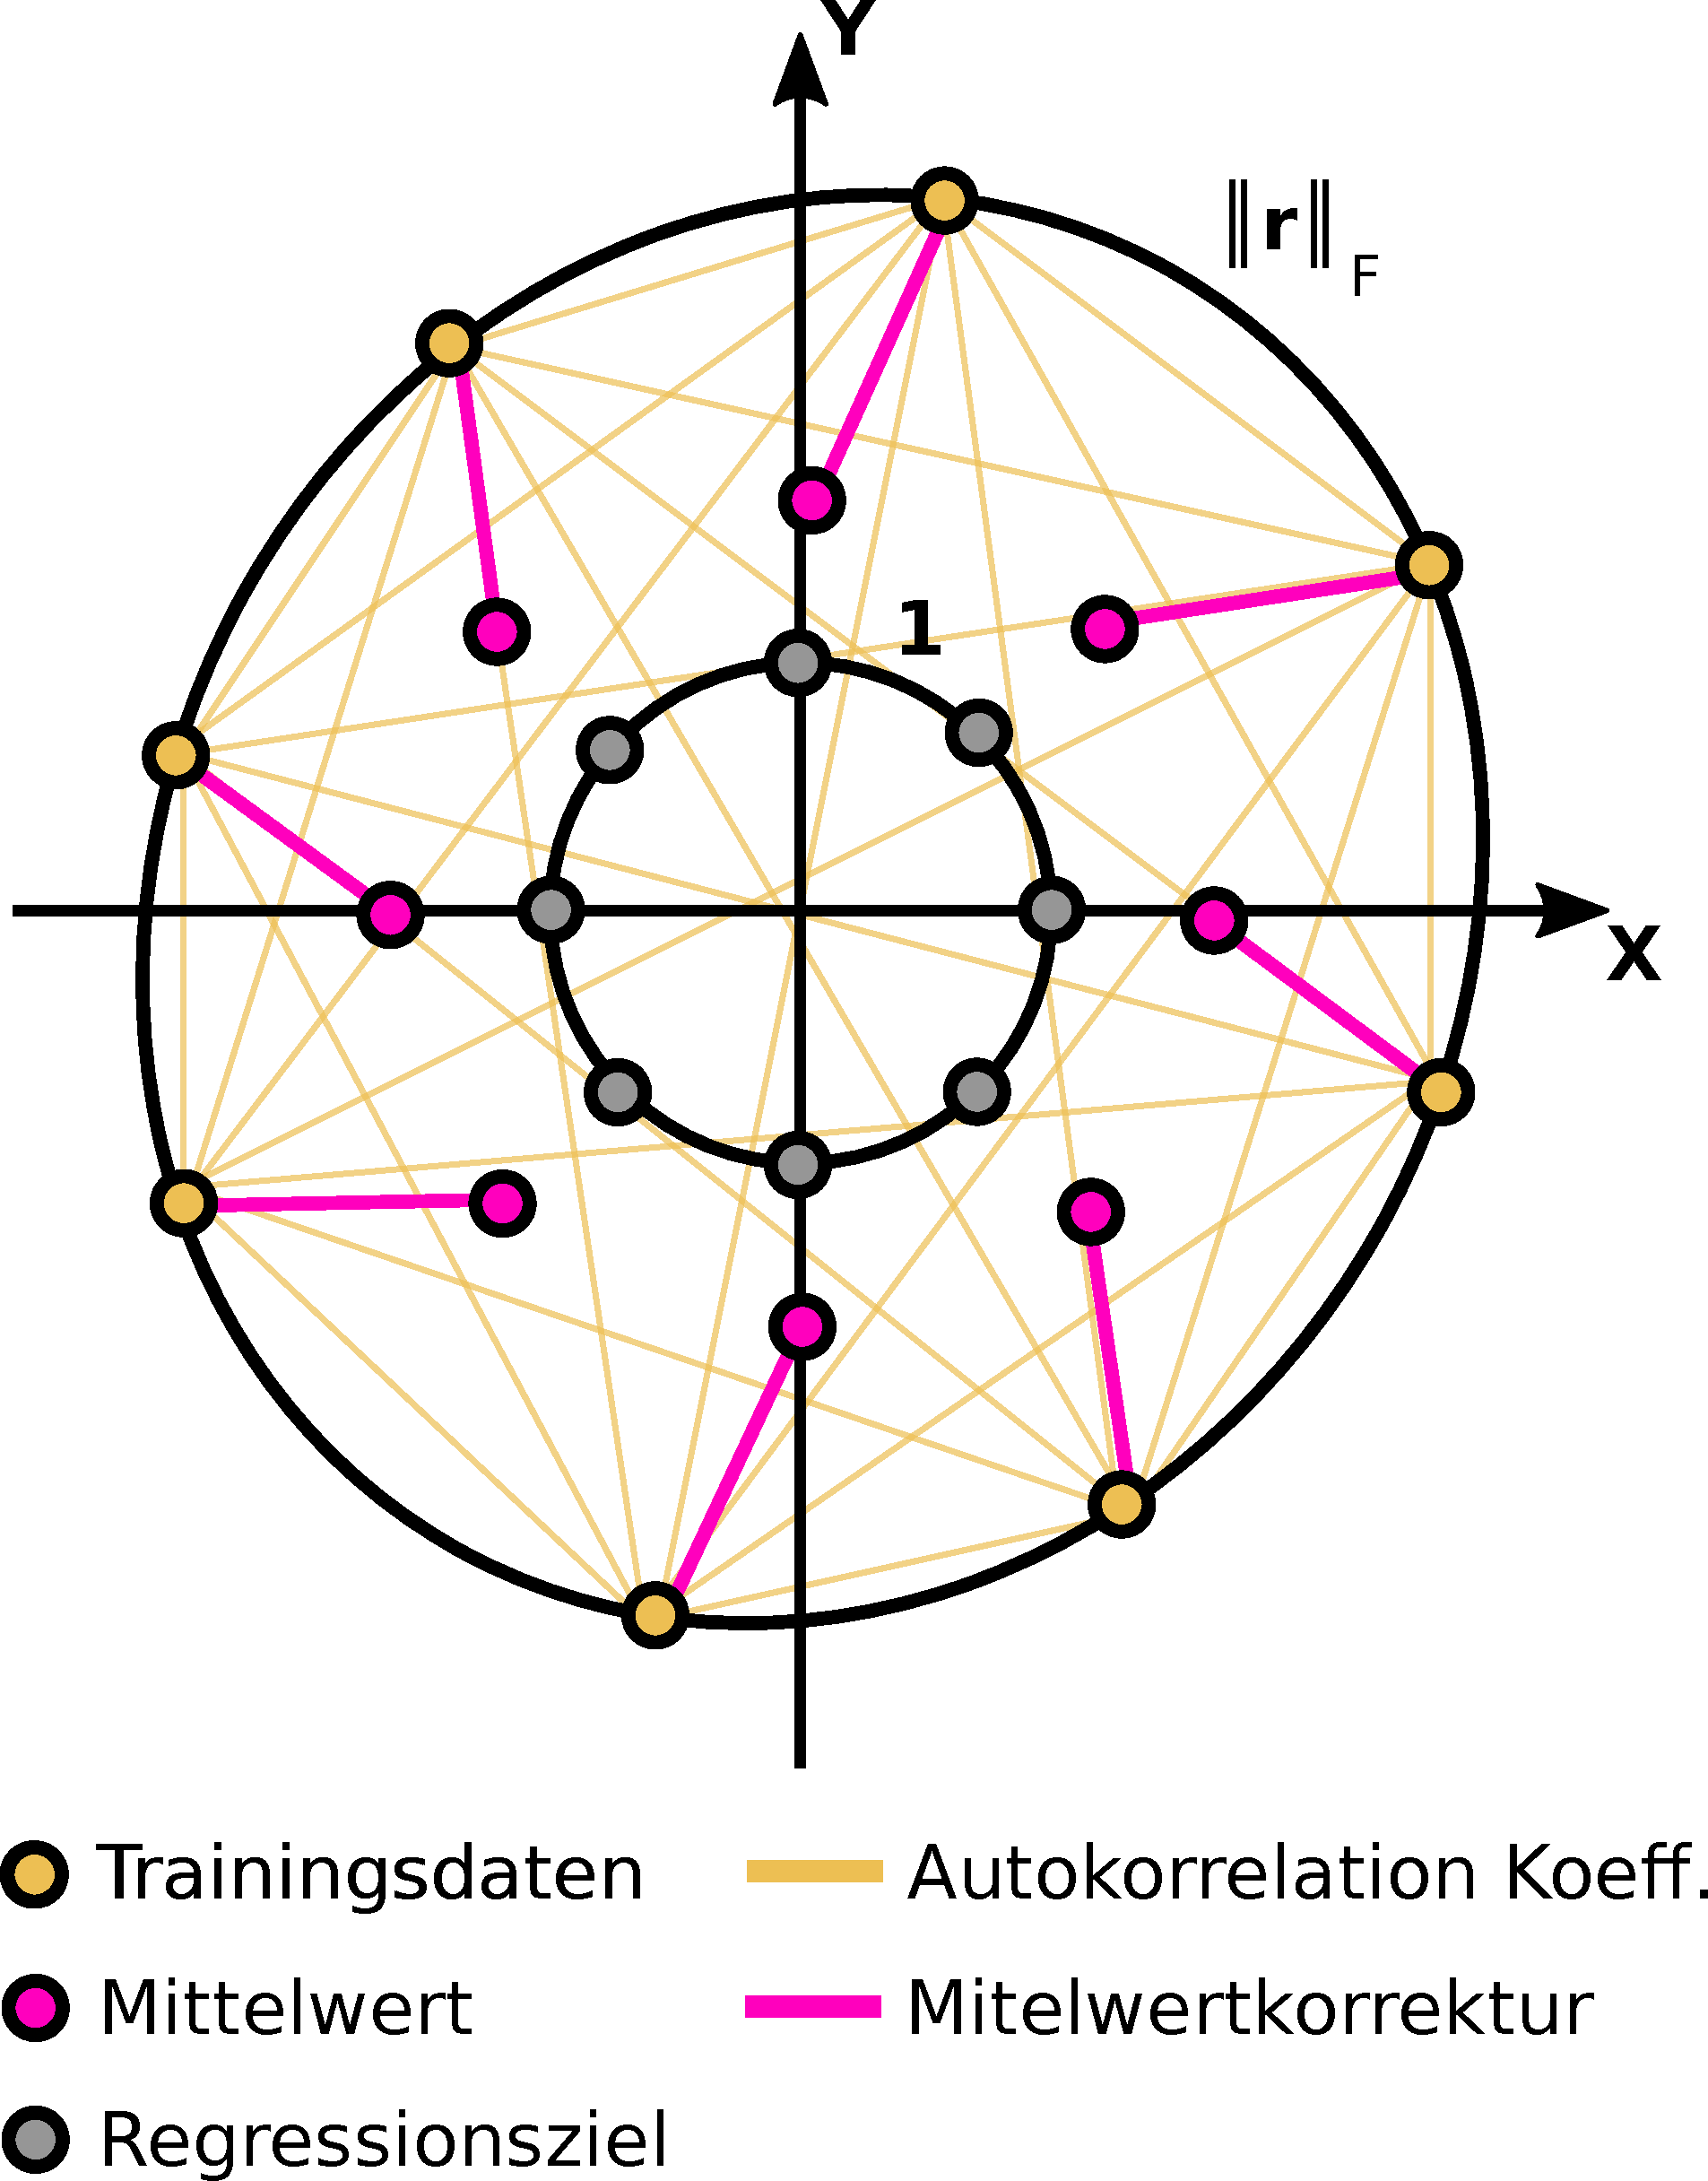
\includegraphics[width=\linewidth]{images/GPR_Mapping_Mean-2}
			\onslide<3>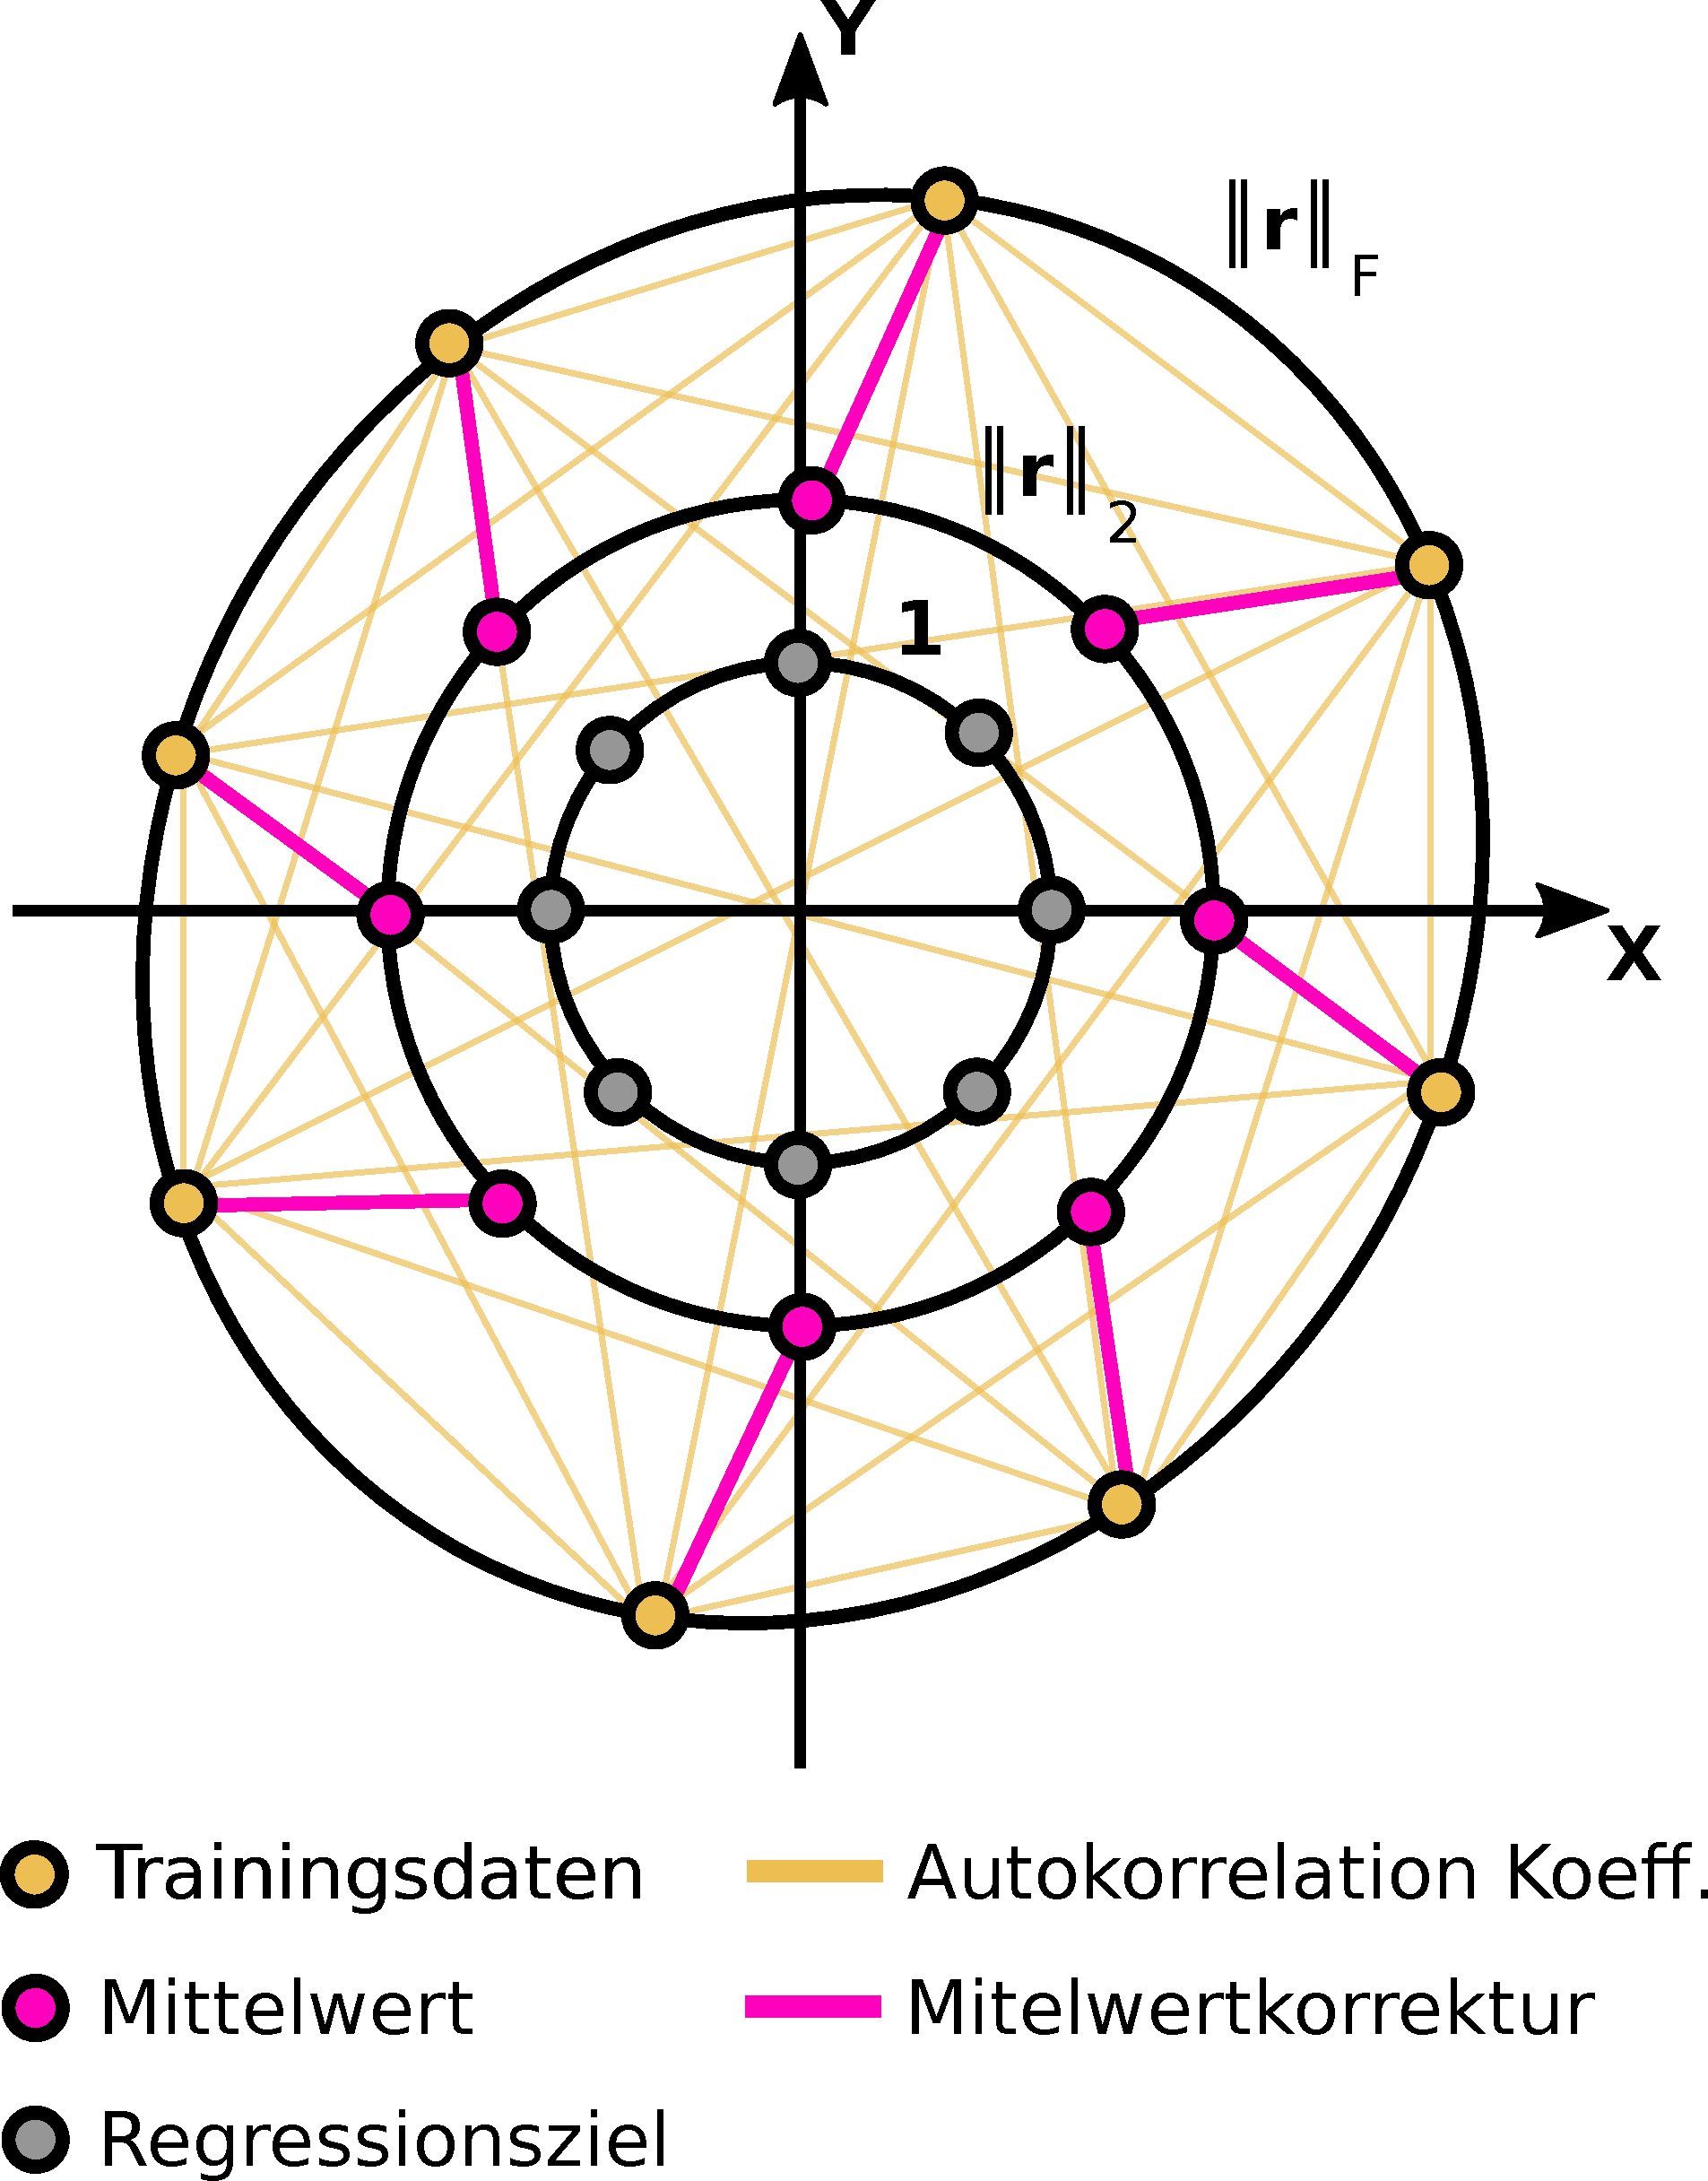
\includegraphics[width=\linewidth]{images/GPR_Mapping_Mean-3}
			\onslide<4>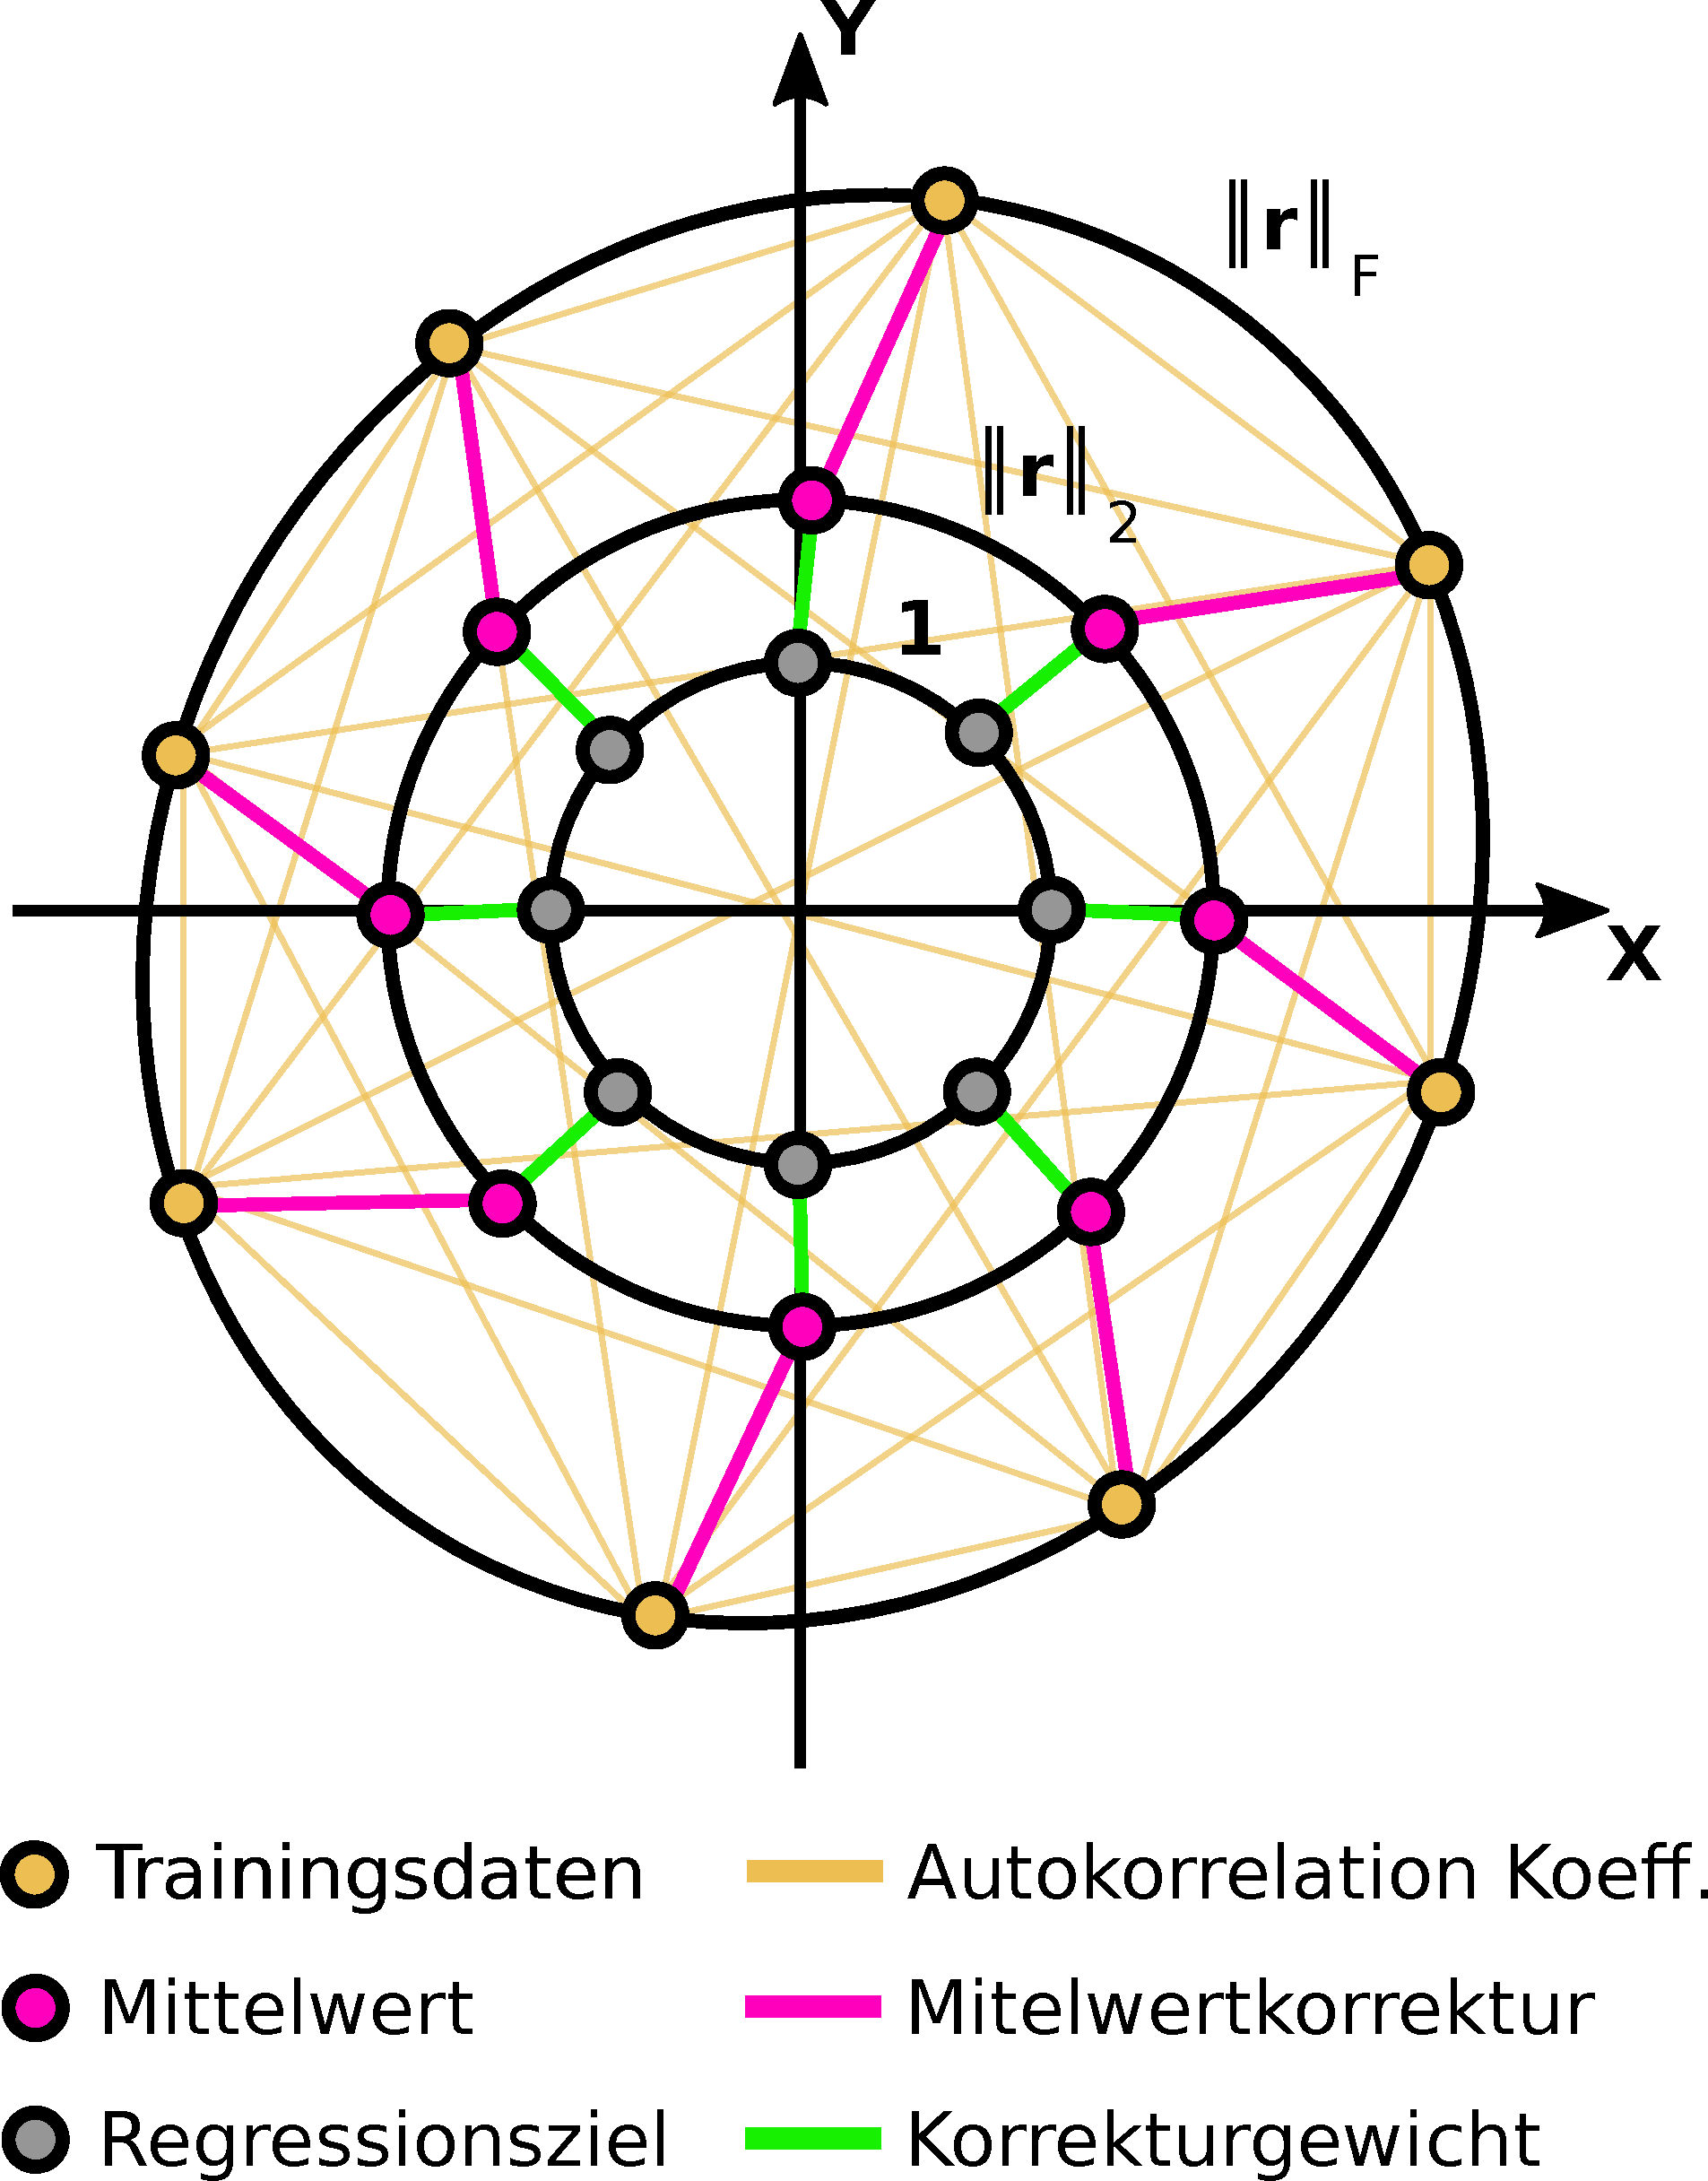
\includegraphics[width=\linewidth]{images/GPR_Mapping_Mean}
		\end{overprint}
	\end{figure}
\end{columns}
\end{frame}
%%%%%%%%%%%%%%%%%%%%%%%%%%%%%%%%%%%%%%%%%%%%%%%%%%%%%%%%%%%%%%%%%%%%%%%%%%%%%%%%%%%%%%%%%%%%%%%%%%%%%%%%%%%%%%%%%%%%%%%%%%%%%%%%%%%%%%%%%
\subsection{GPR-Trainingsphase}
\begin{frame}
\frametitle{GPR-Verfahren}
\framesubtitle{GPR-Trainingsphase}
\begin{figure}
	\begin{overprint}
		\onslide<1>\centering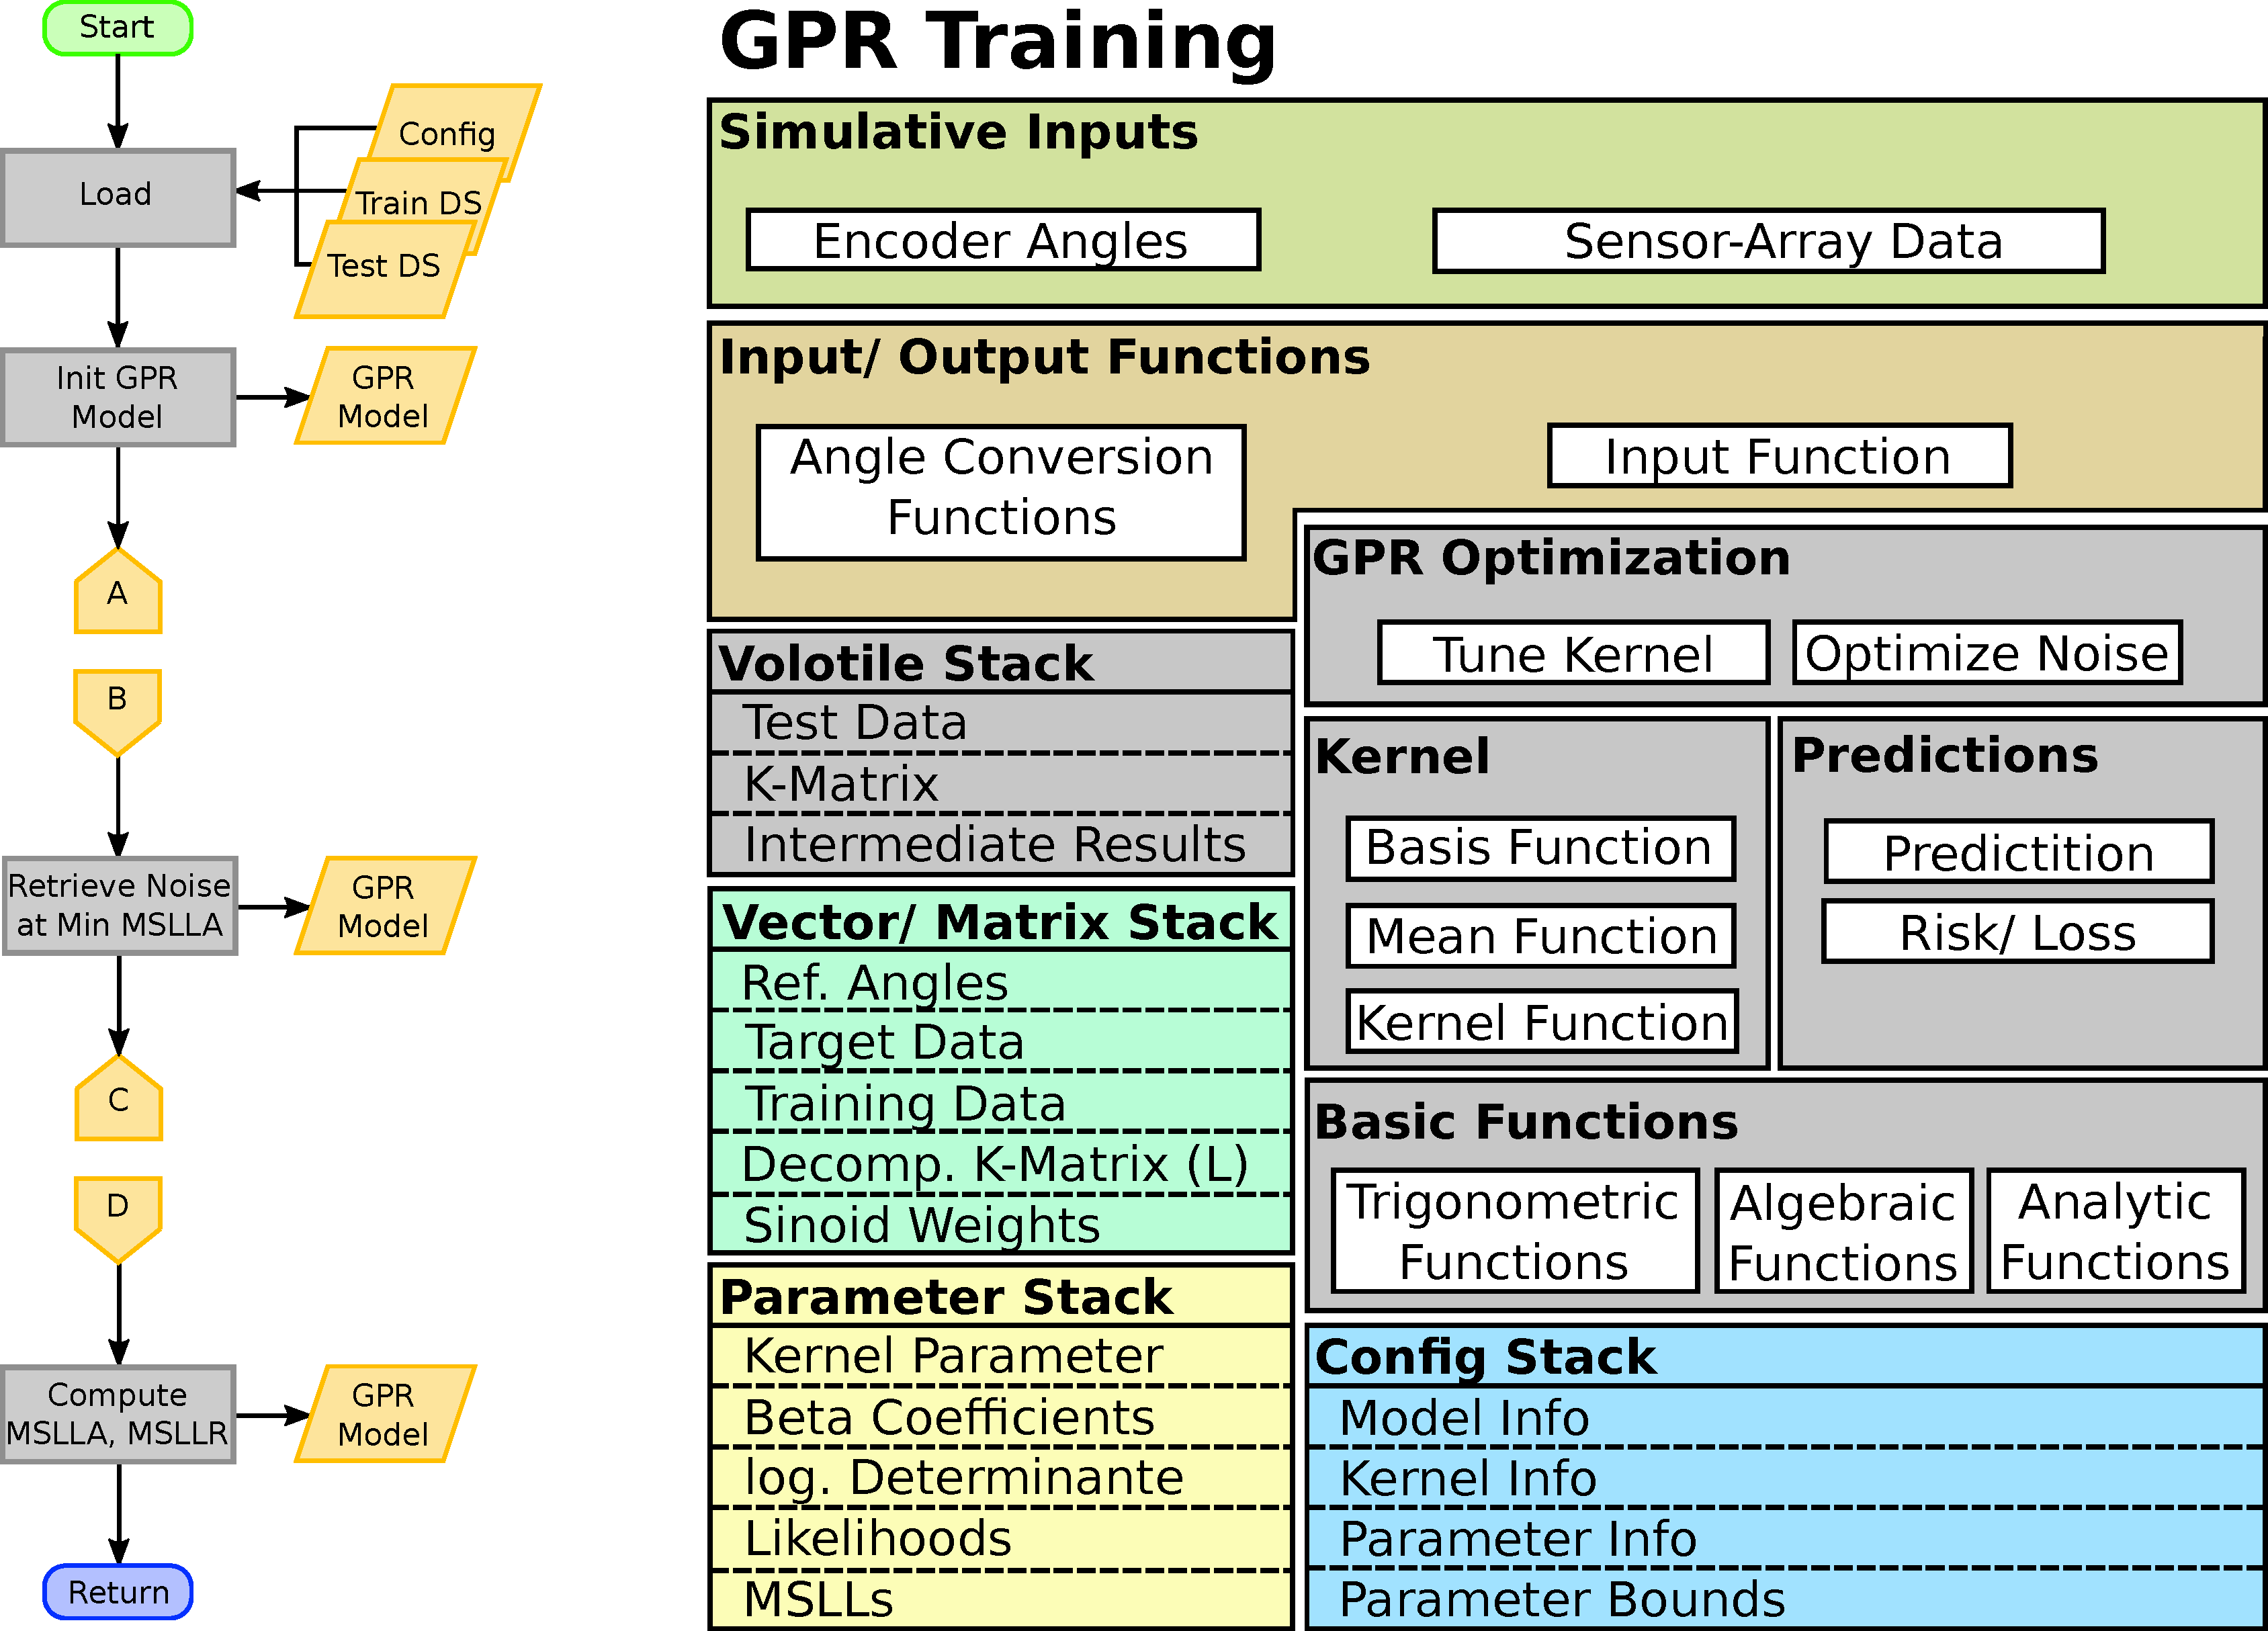
\includegraphics[width=.8\linewidth]{images/GPR_Trainingsphase-1}
		\onslide<2>\centering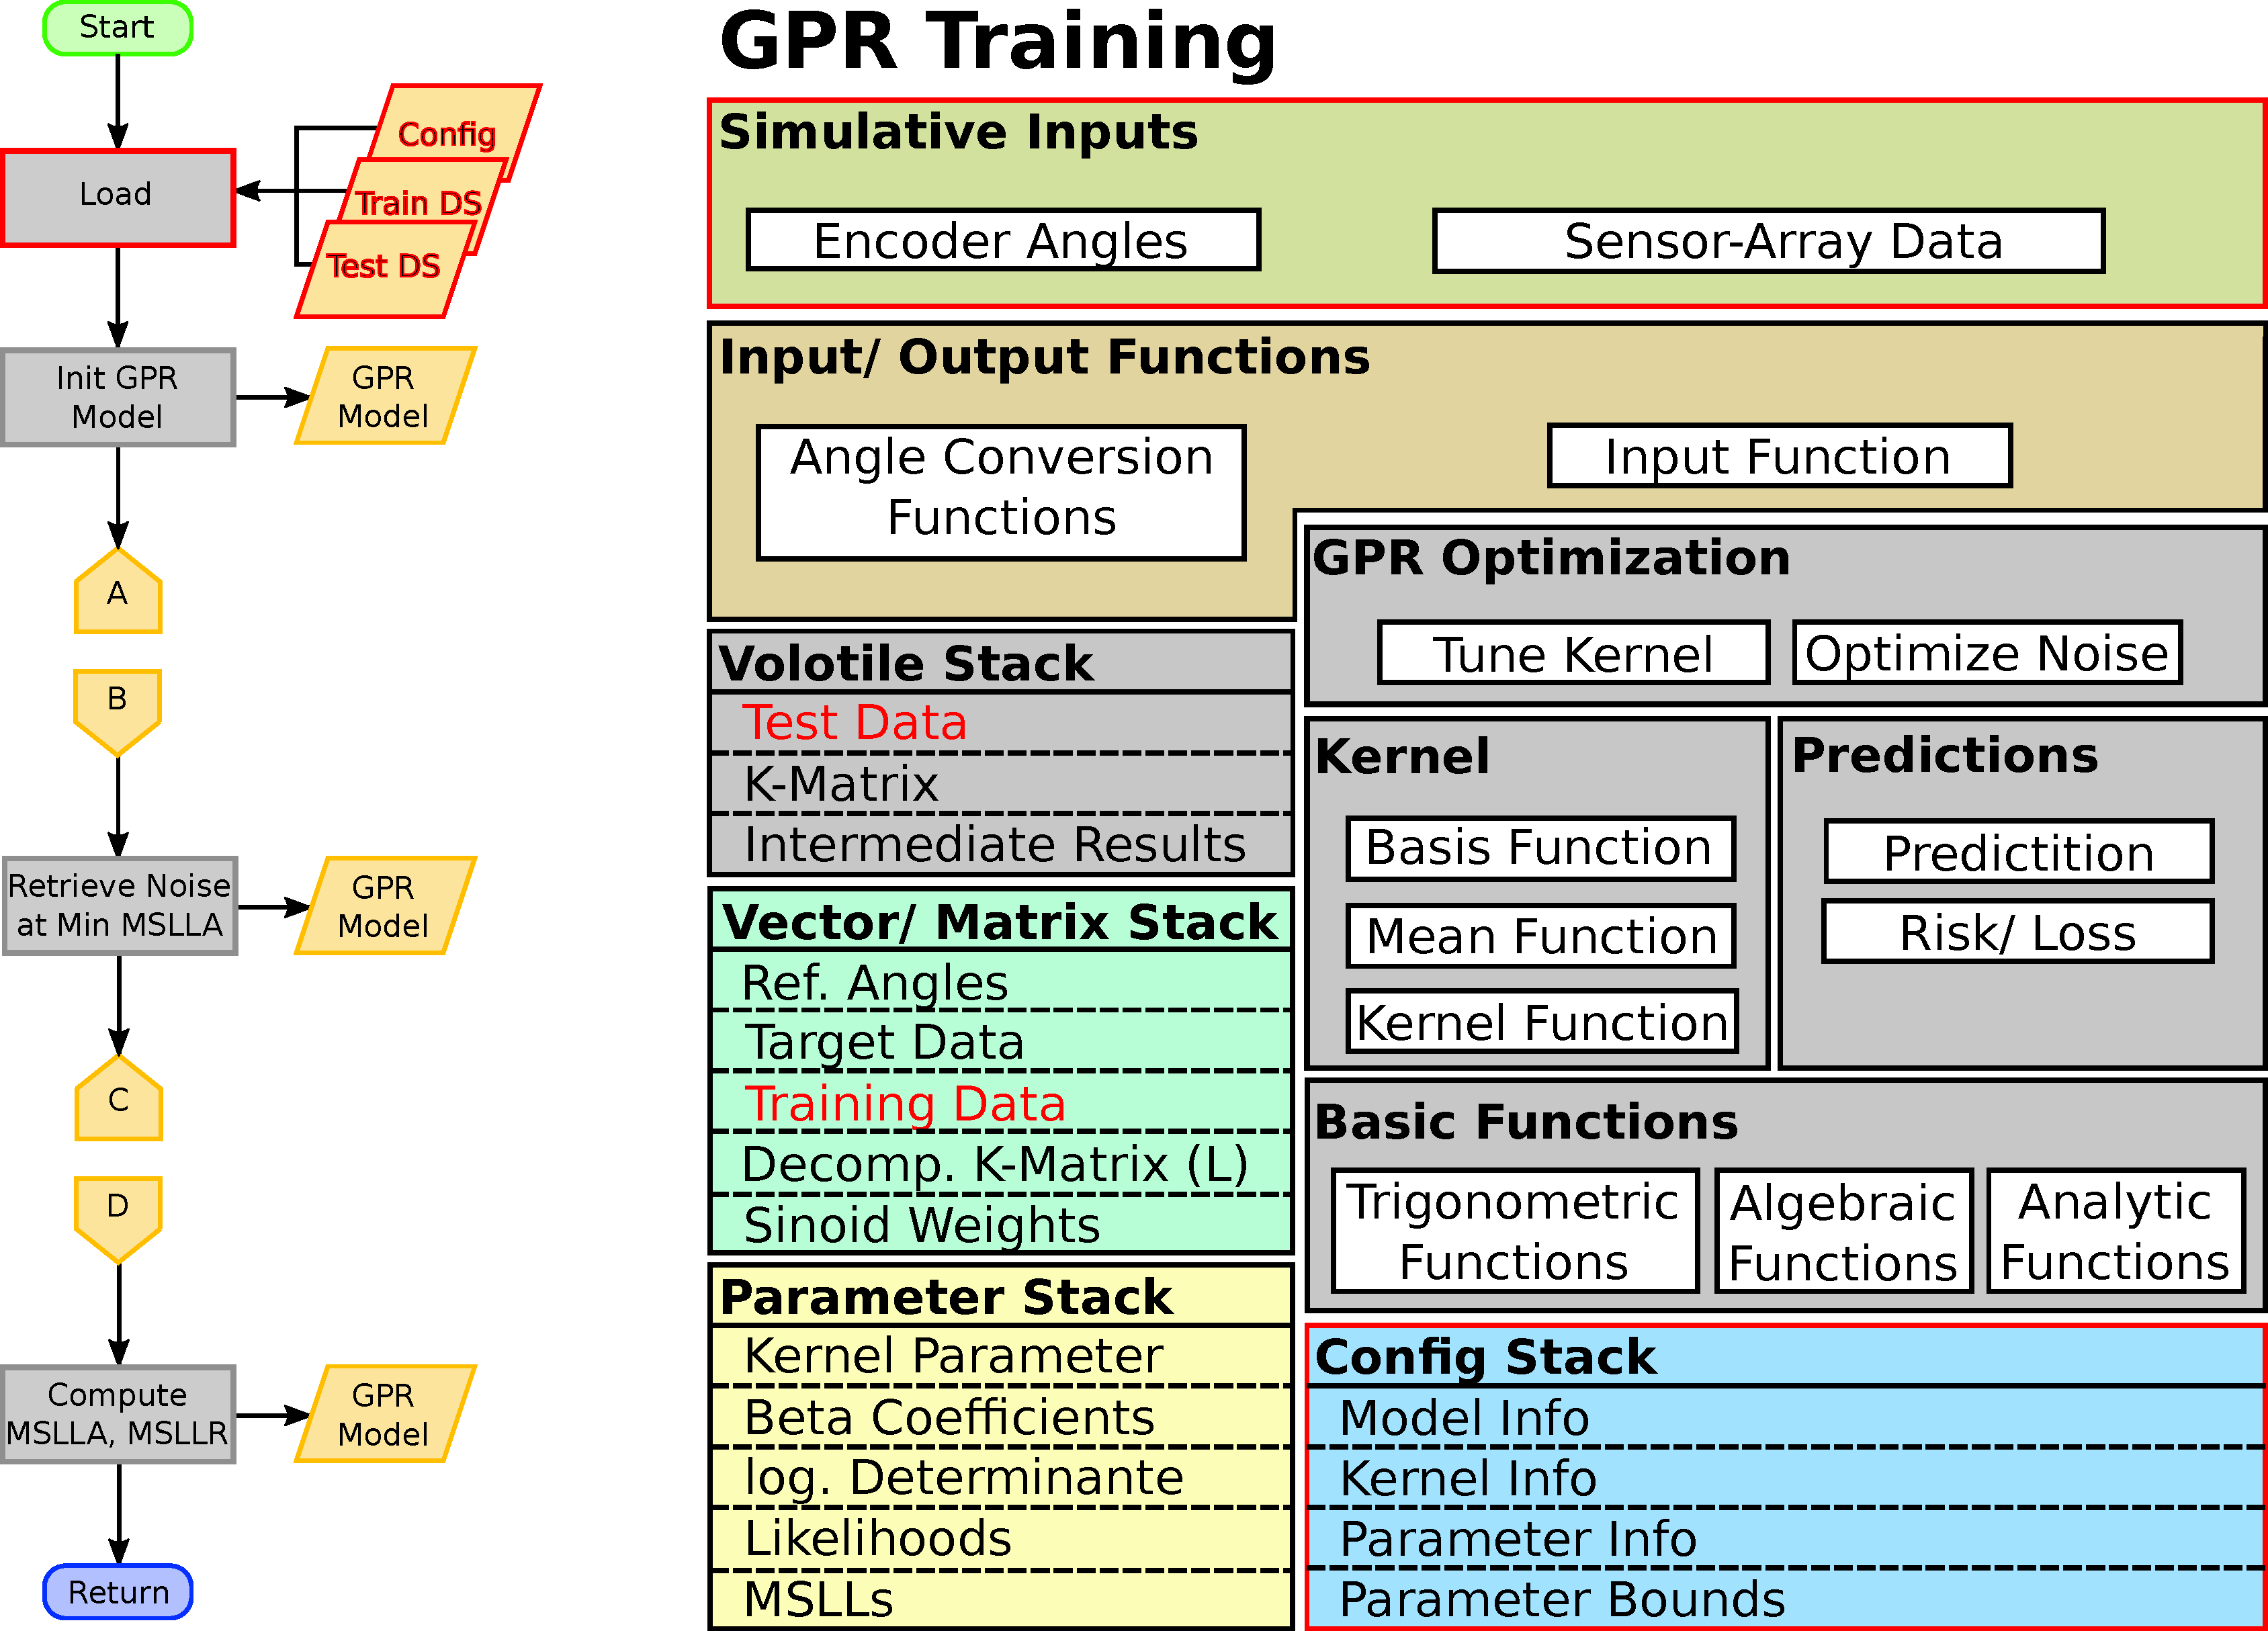
\includegraphics[width=.8\linewidth]{images/GPR_Trainingsphase-2}
		\onslide<3>\centering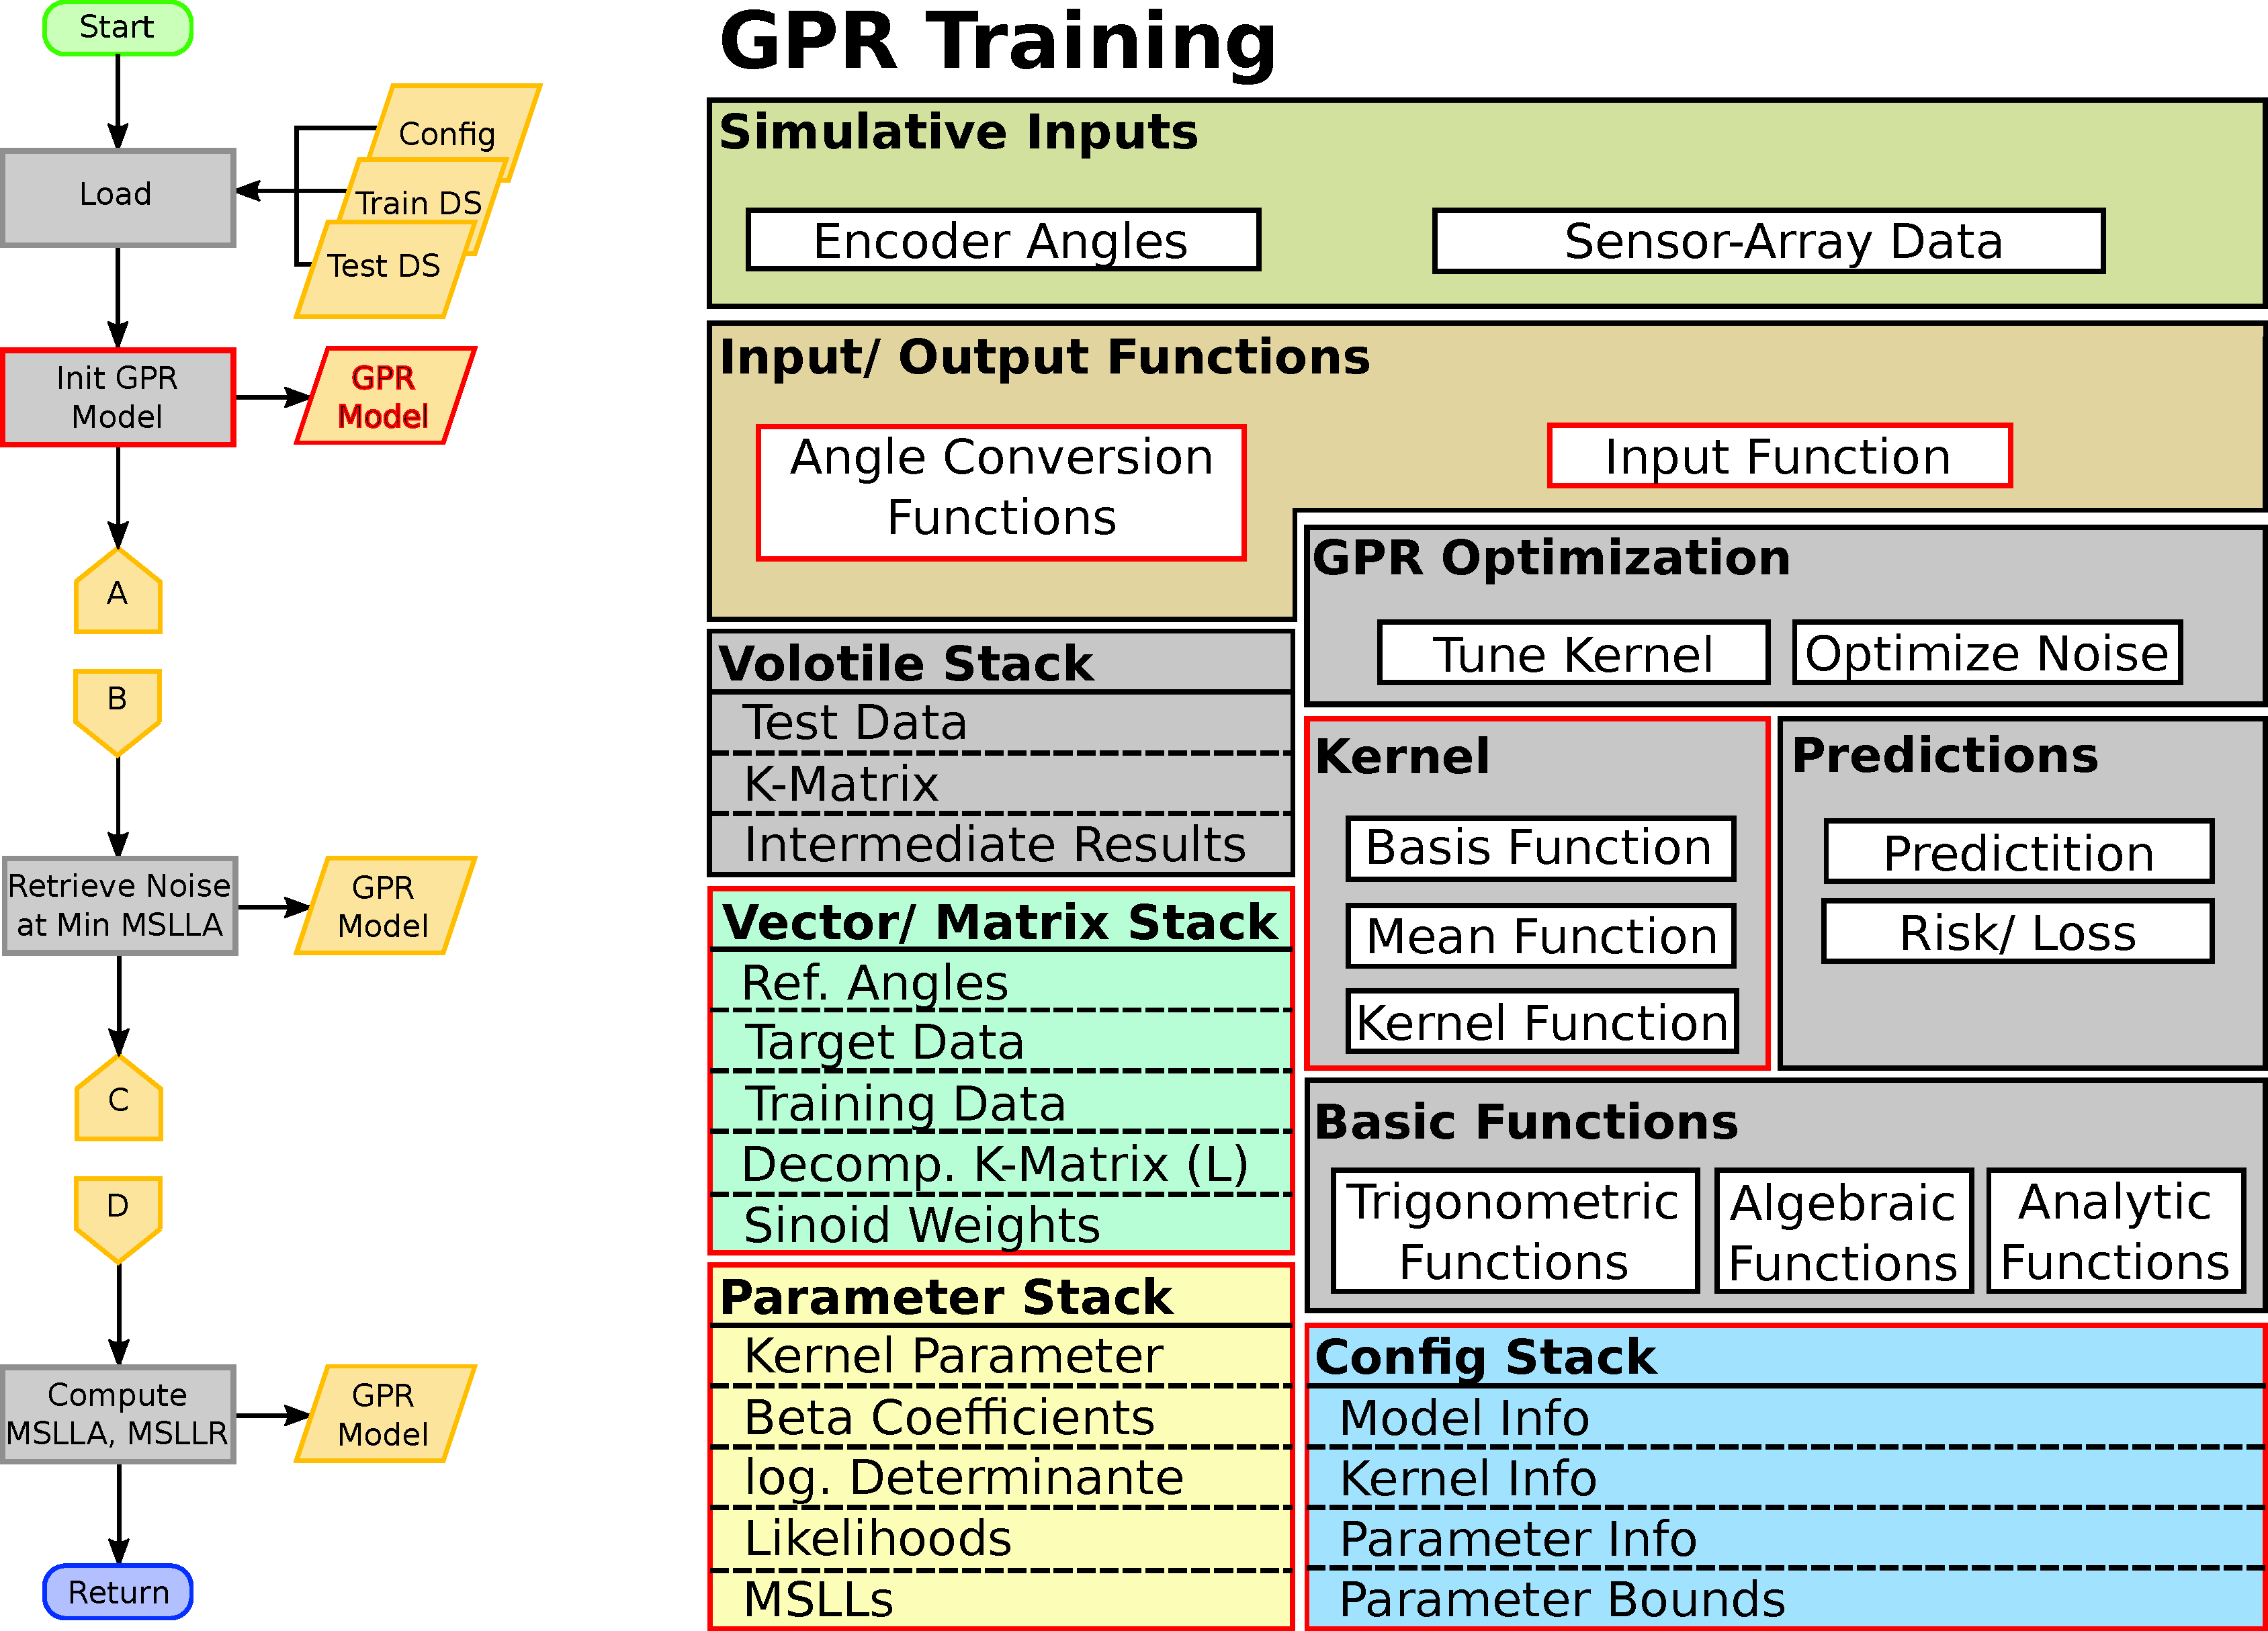
\includegraphics[width=.8\linewidth]{images/GPR_Trainingsphase-3}
	\end{overprint}
\end{figure}
\end{frame}
%%%%%%%%%%%%%%%%%%%%%%%%%%%%%%%%%%%%%%%%%%%%%%%%%%%%%%%%%%%%%%%%%%%%%%%%%%%%%%%%%%%%%%%%%%%%%%%%%%%%%%%%%%%%%%%%%%%%%%%%%%%%%%%%%%%%%%%%%
\begin{frame}
\frametitle{GPR-Verfahren}
\framesubtitle{GPR-Trainingsphase}
\textbf{Init GPR:}
\begin{columns}[c]
	\column{.35\textwidth}
	\begin{itemize}
		\item<1-> MAT-Dateien, Struct
		\item<2-> Infos, Bounds, etc.
		\item<3-> Einheitskreis, Bezüge
		\item<4-> Module, Data-Fit
		\item<5-> GPR Parametrierung
	\end{itemize}
	\column{.6\textwidth}
	\begin{figure}
		\begin{overprint}
			\onslide<1>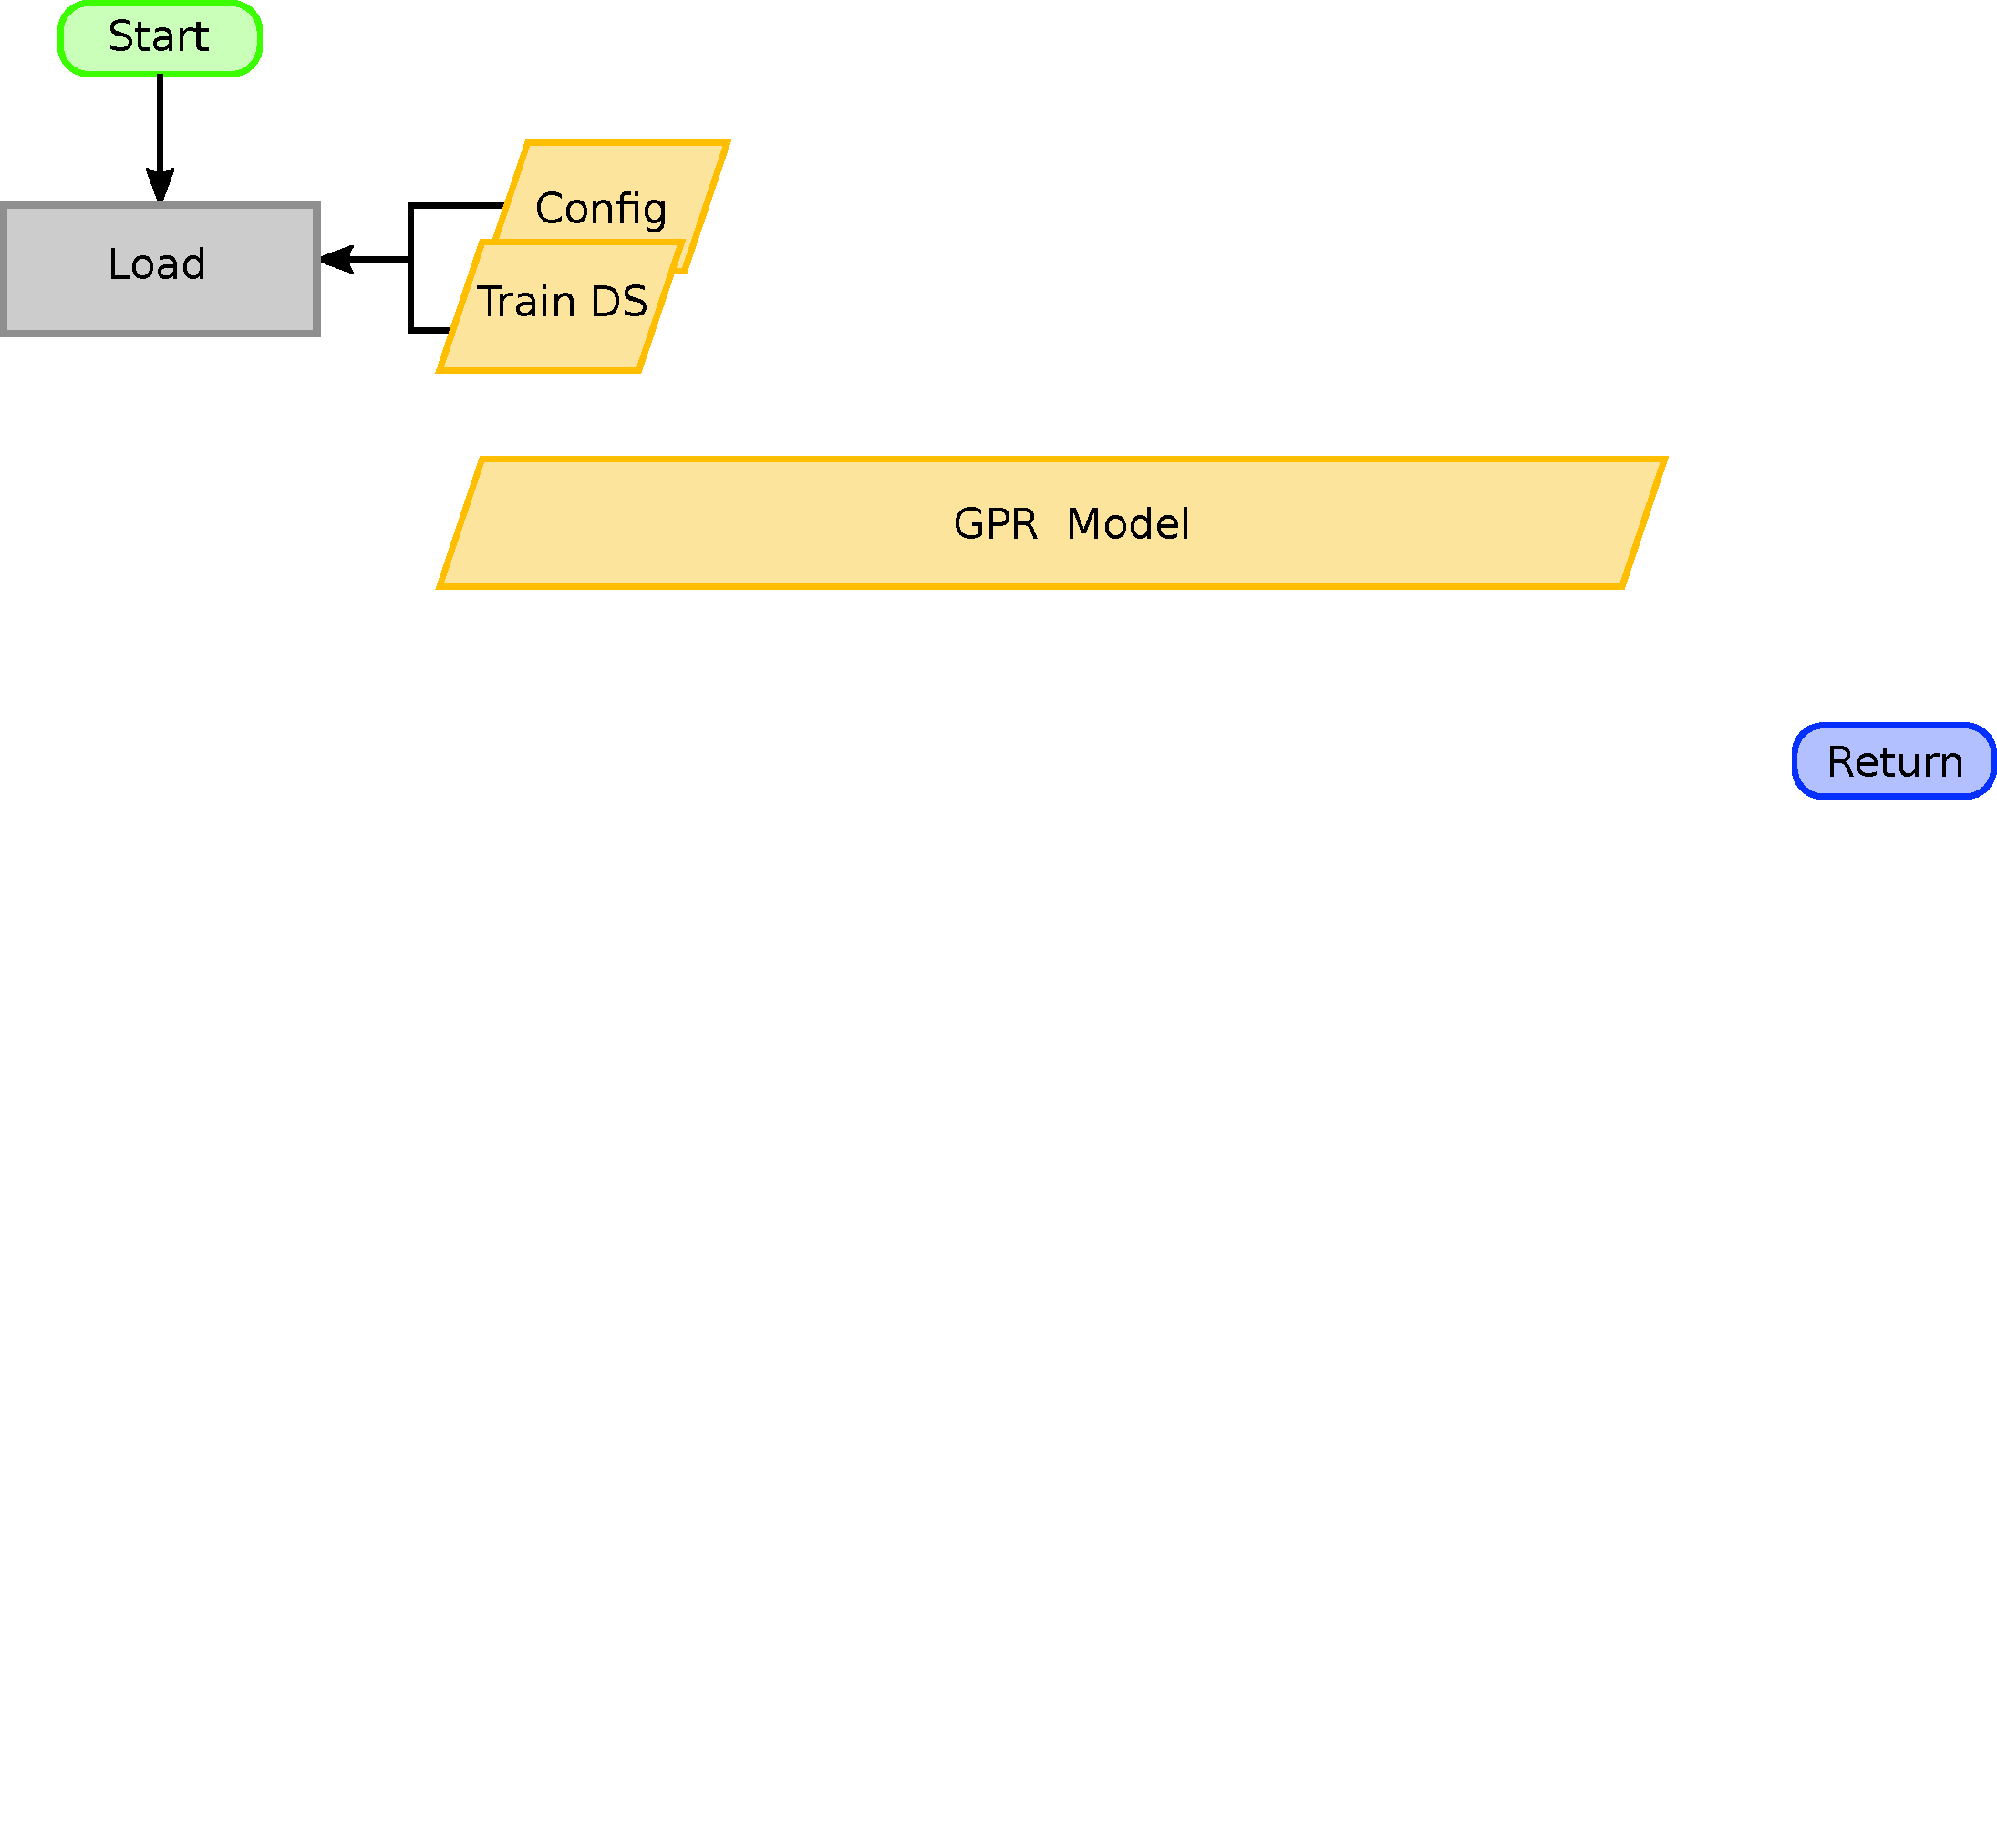
\includegraphics[width=\linewidth]{images/GPR_Initialization-1}
			\onslide<2>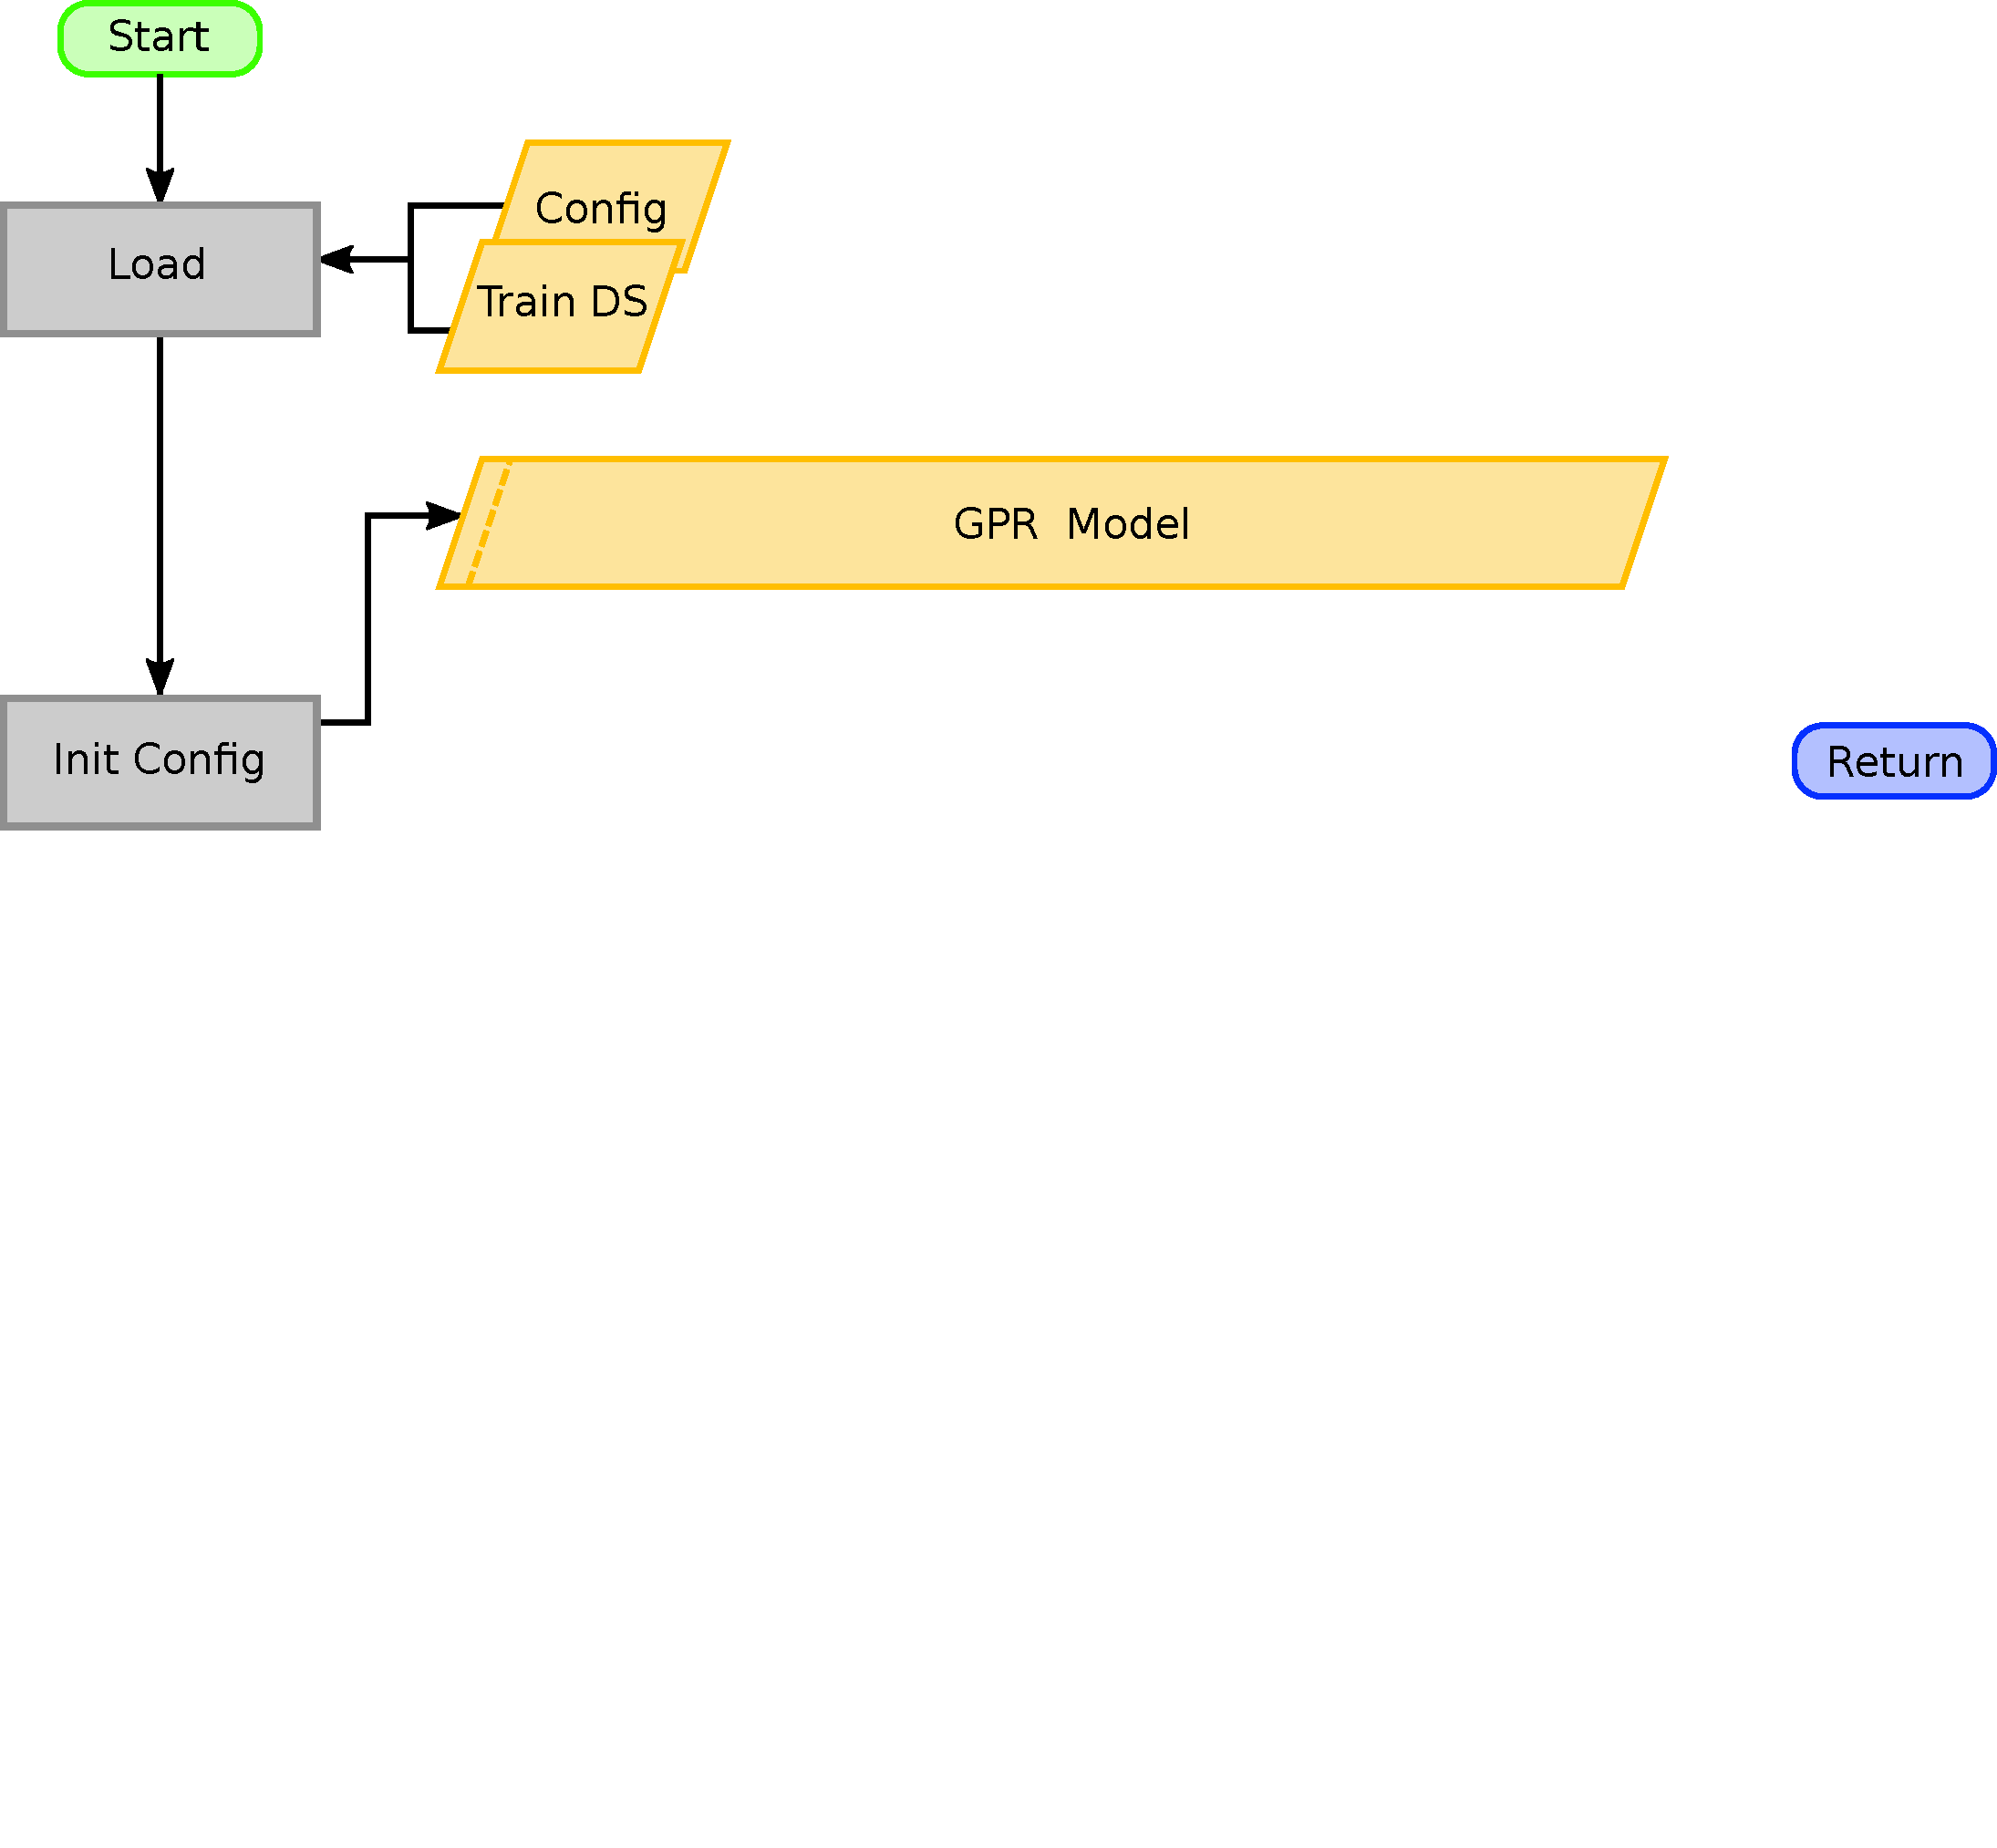
\includegraphics[width=\linewidth]{images/GPR_Initialization-2}
			\onslide<3>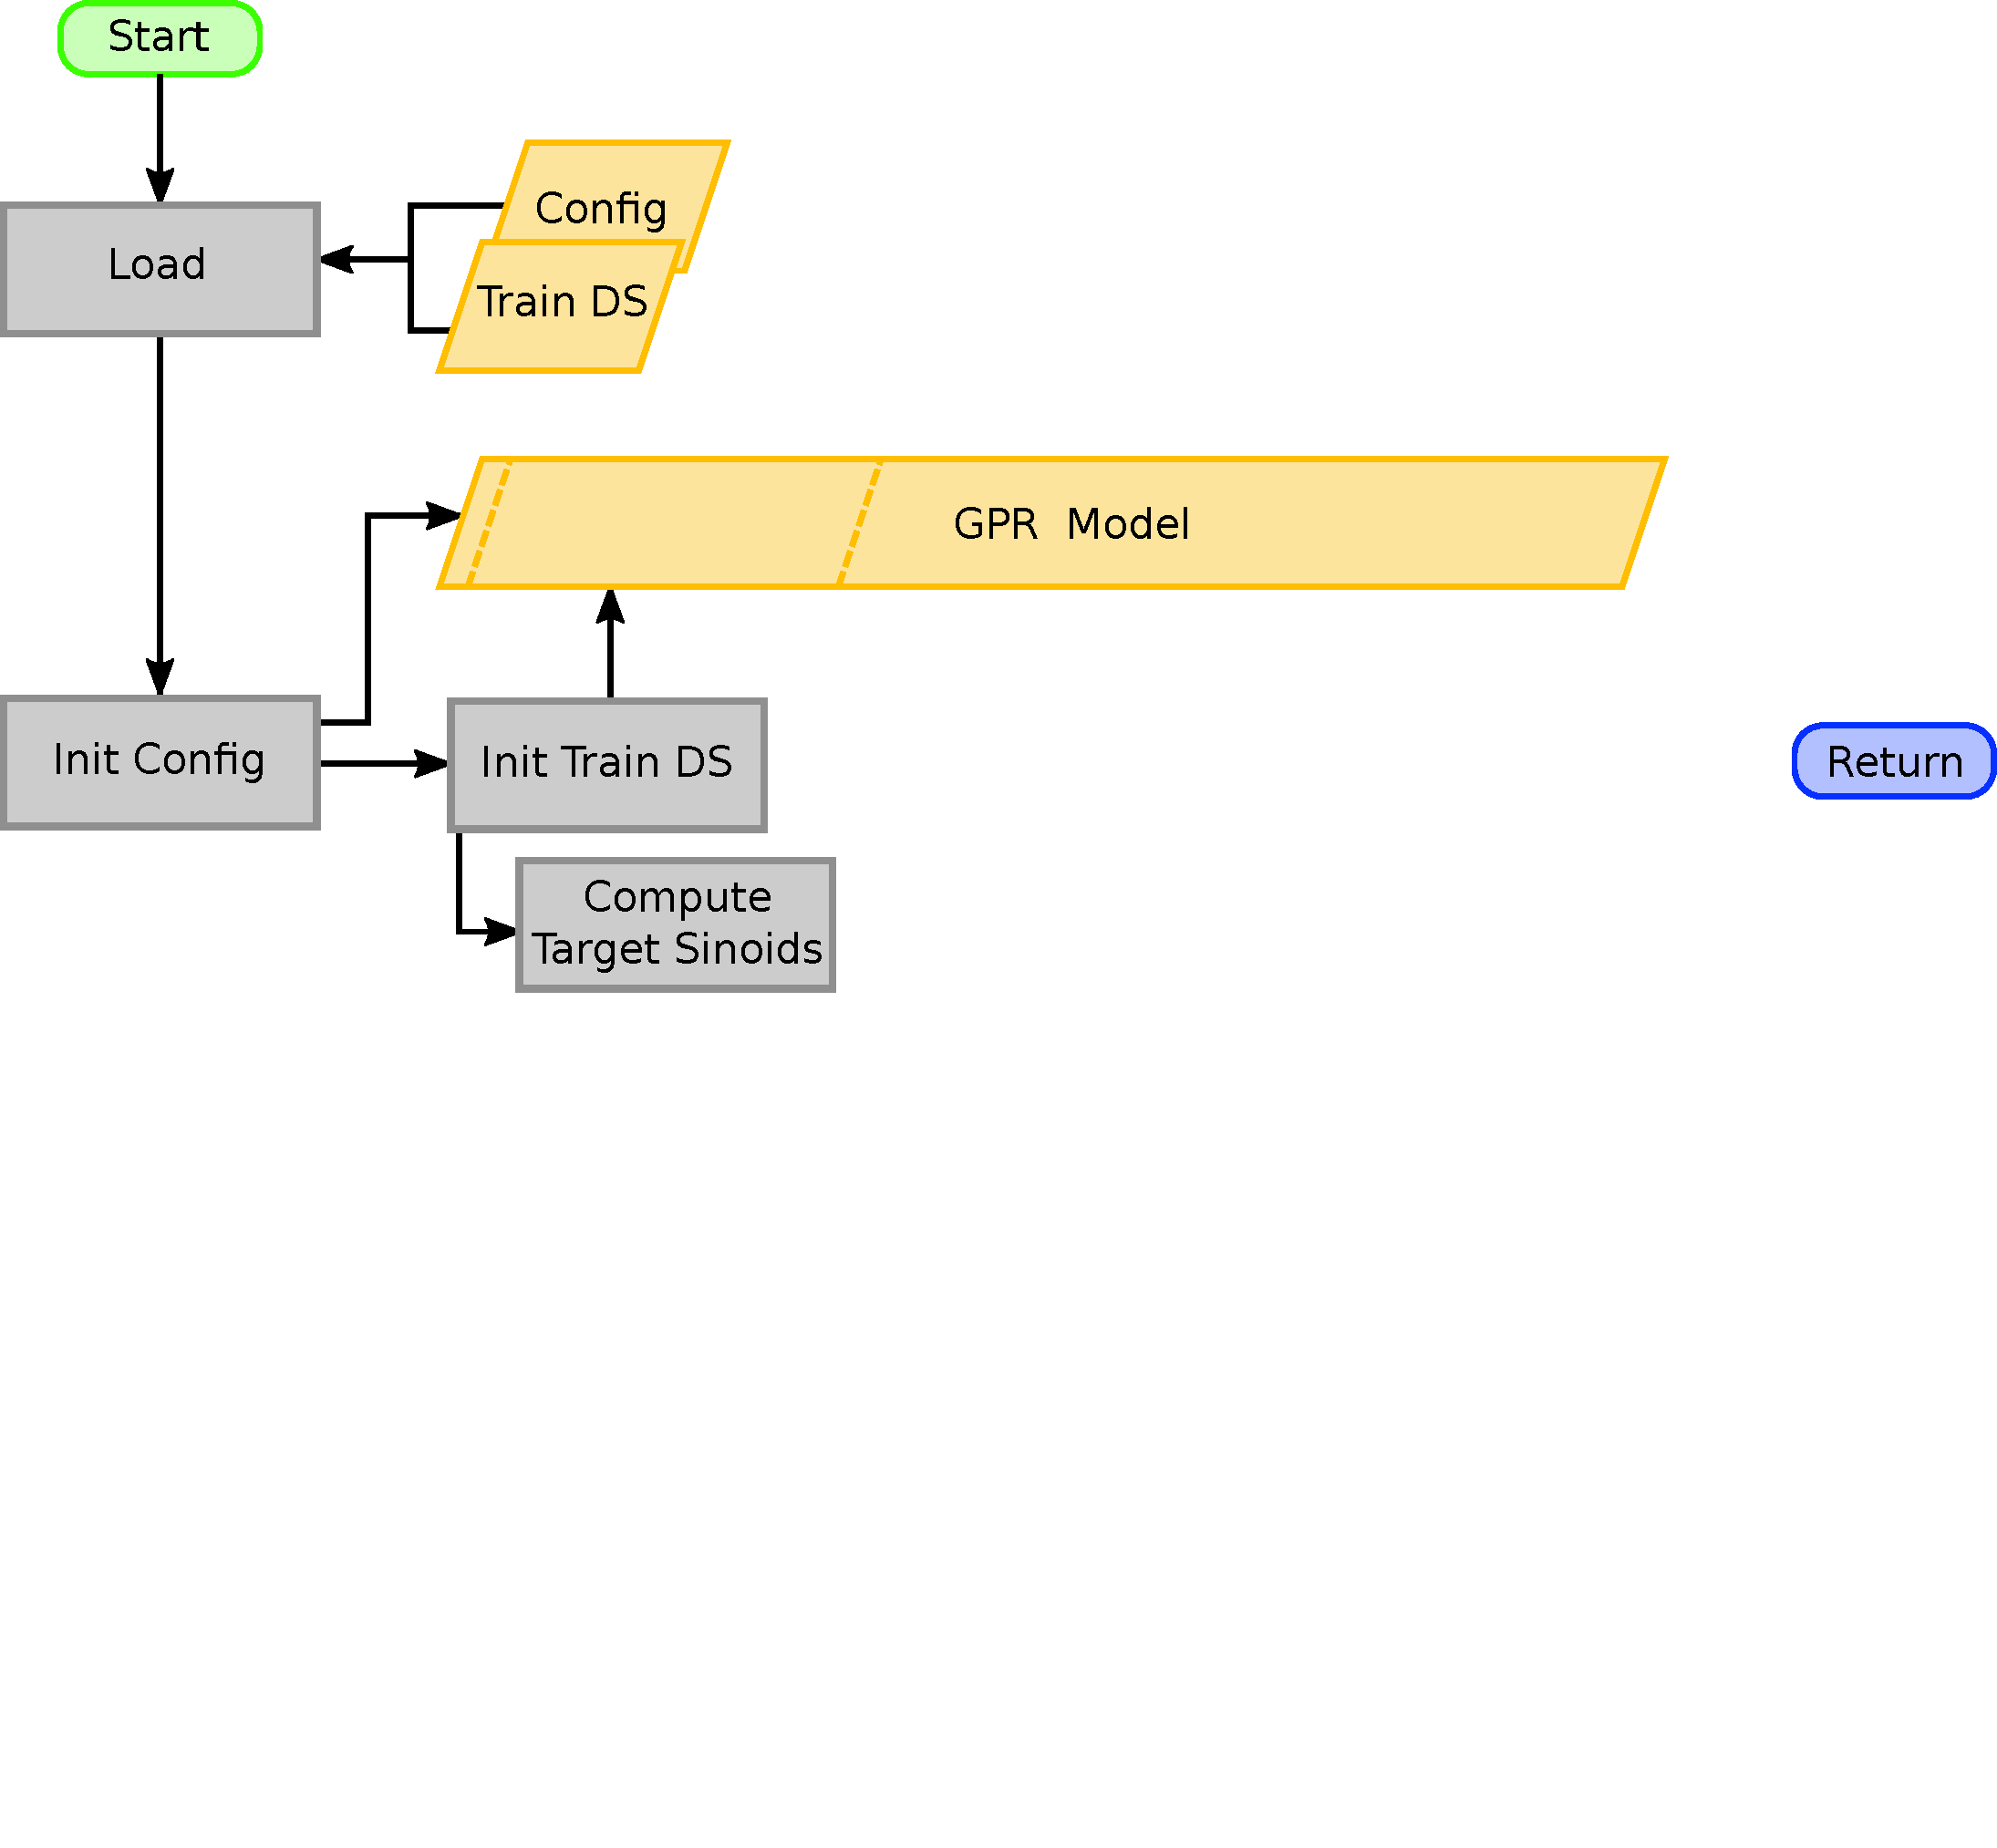
\includegraphics[width=\linewidth]{images/GPR_Initialization-3}
			\onslide<4>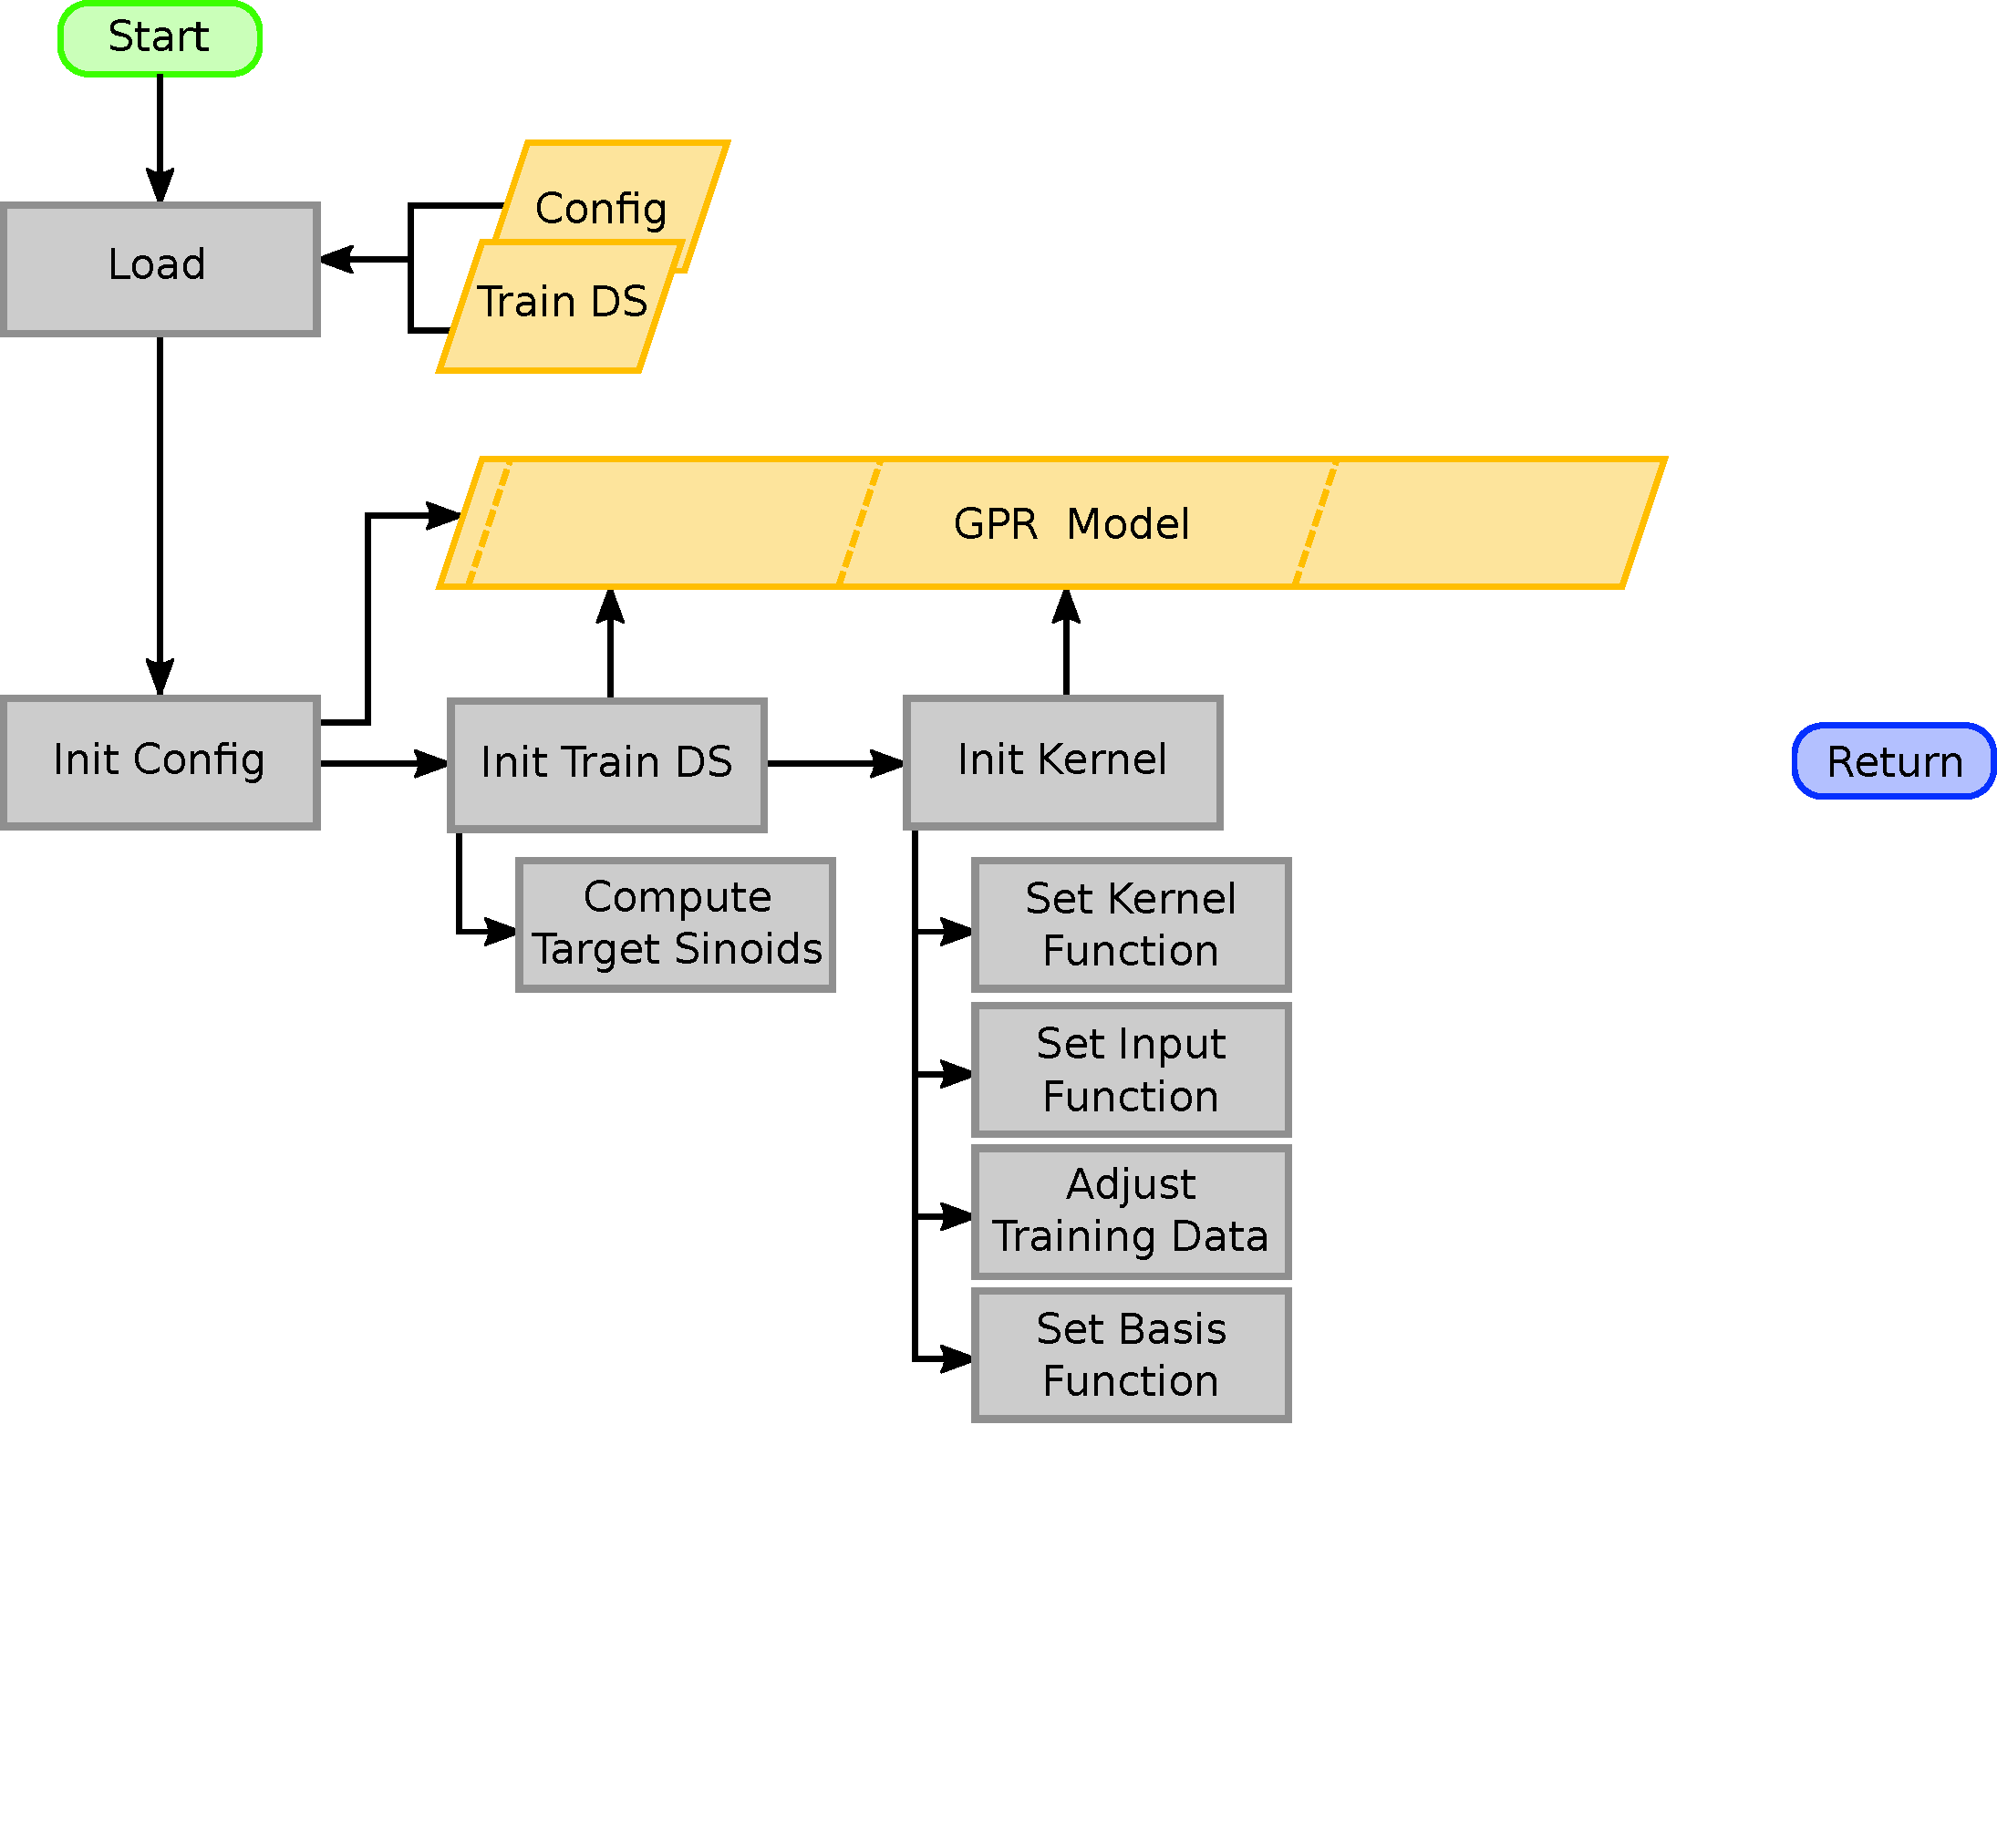
\includegraphics[width=\linewidth]{images/GPR_Initialization-4}
			\onslide<5>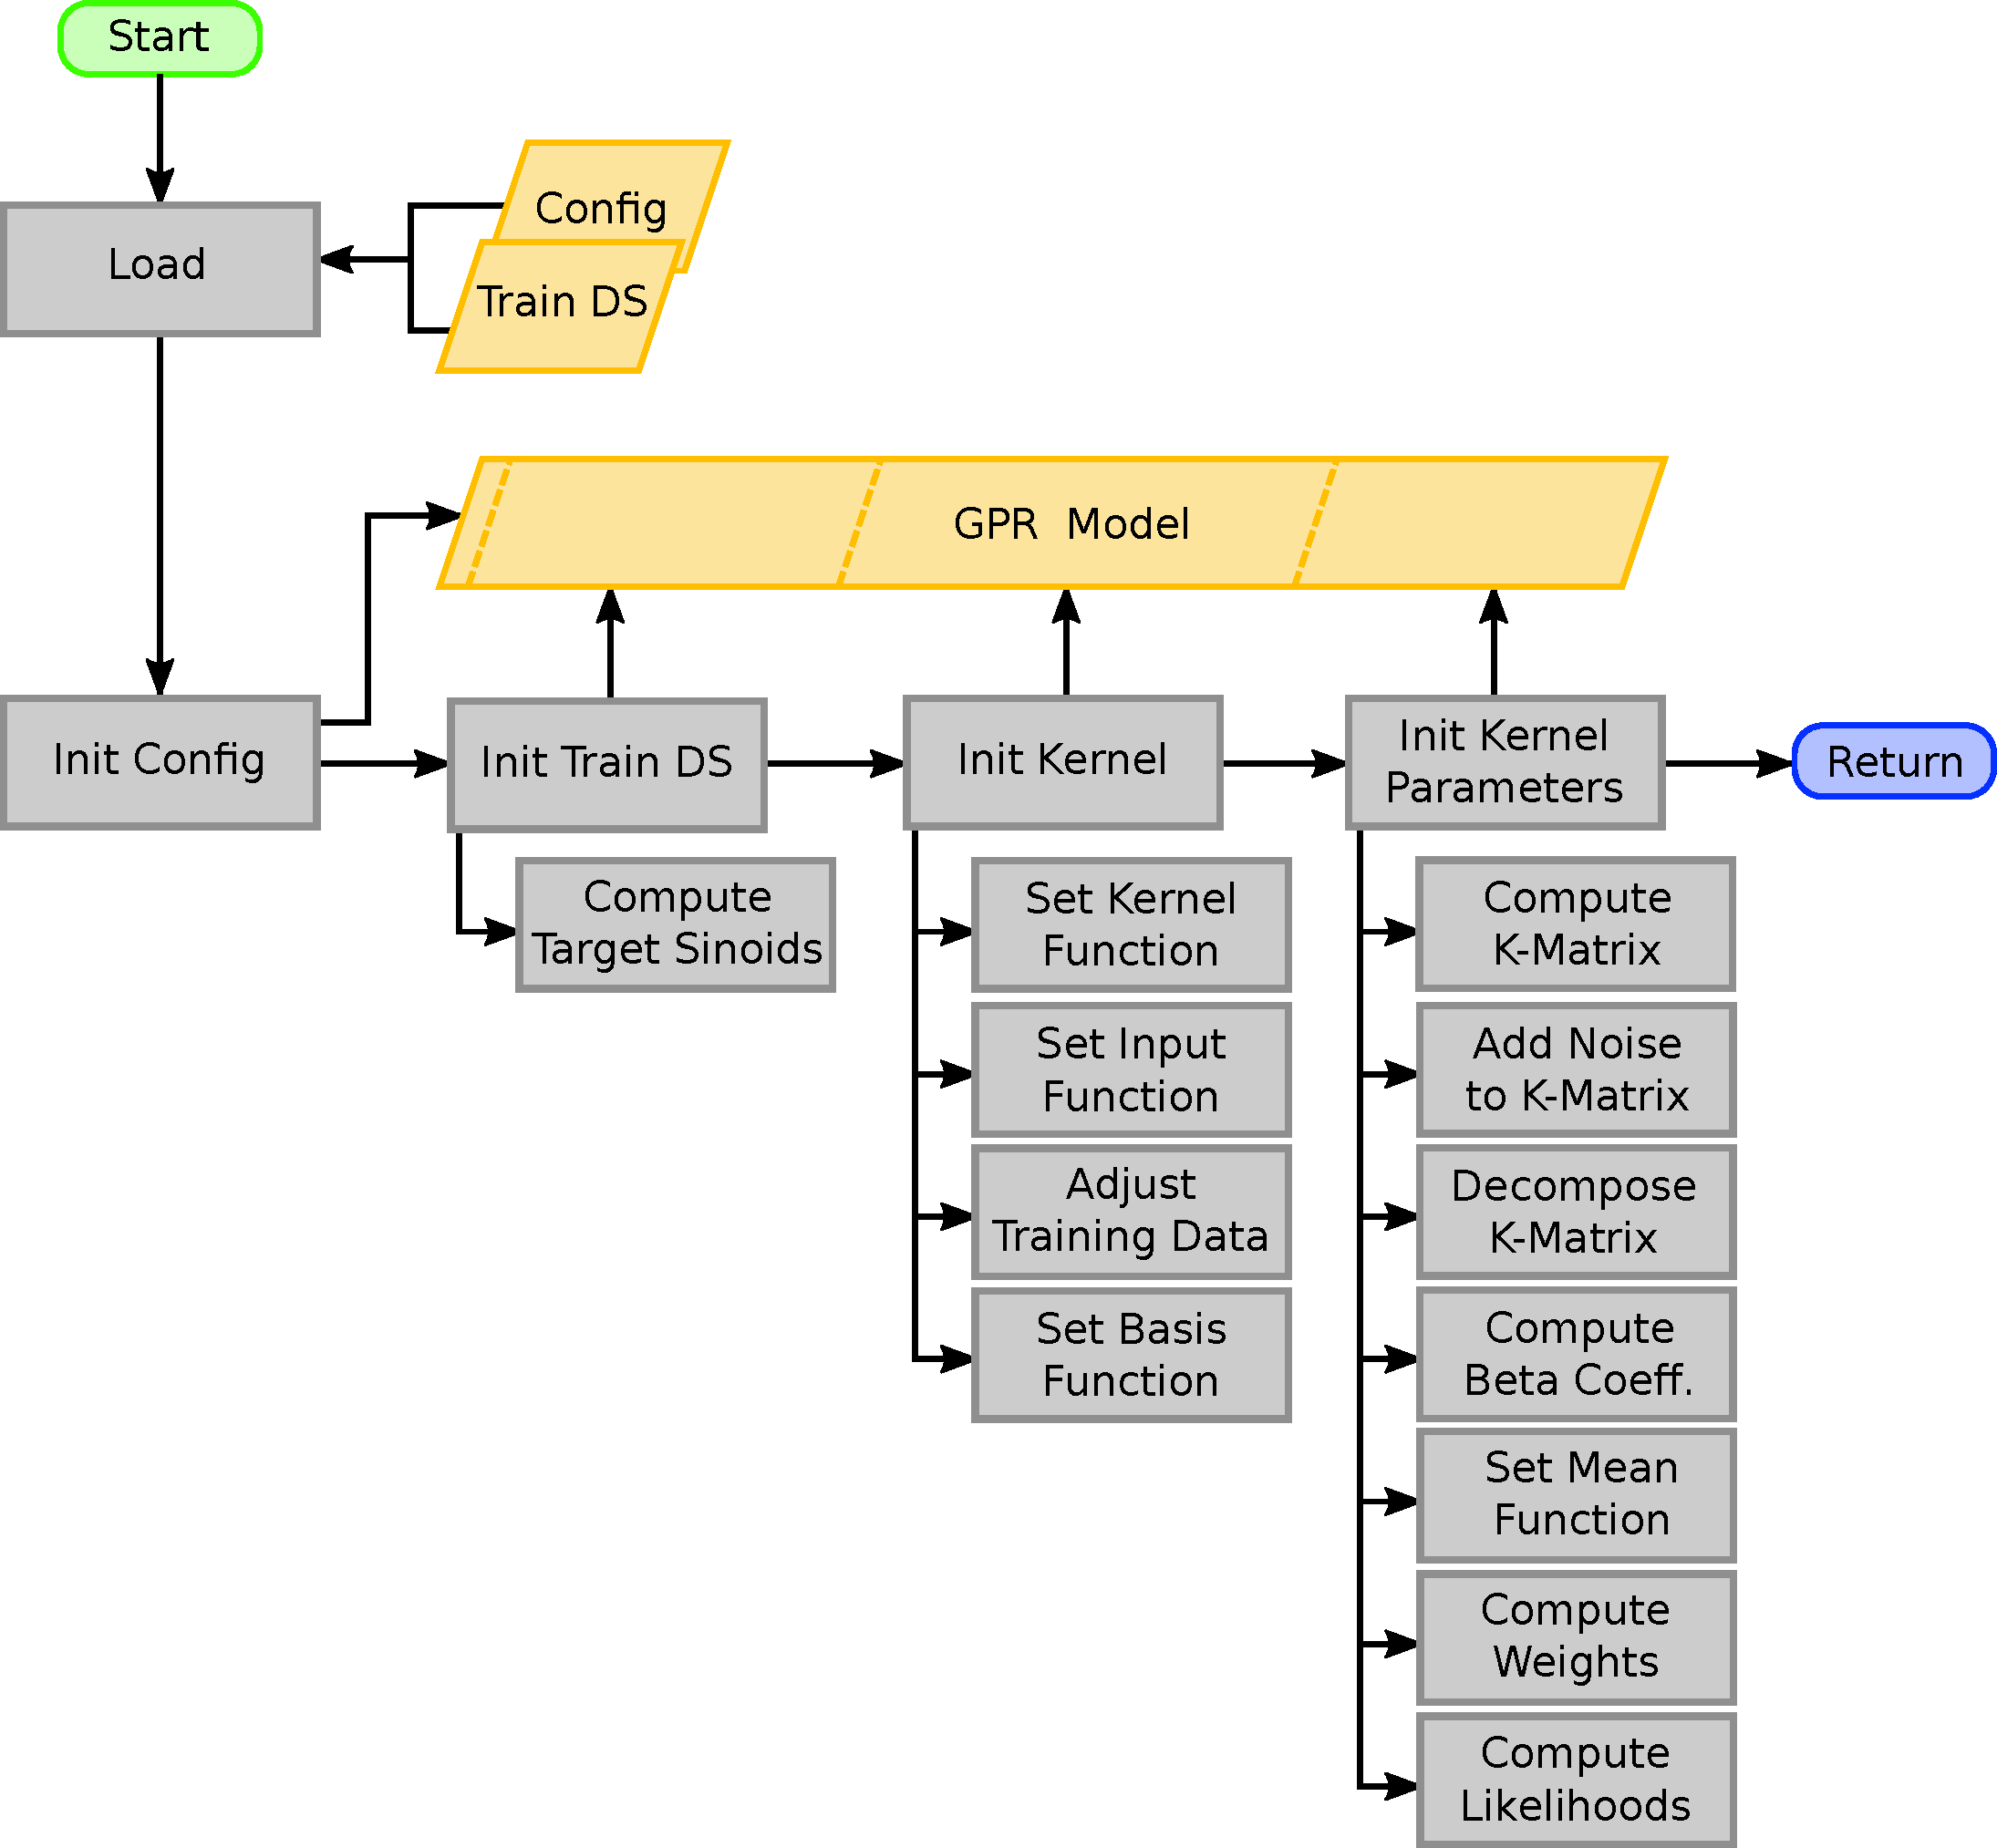
\includegraphics[width=\linewidth]{images/GPR_Initialization}
		\end{overprint}
	\end{figure}
\end{columns}
\end{frame}
%%%%%%%%%%%%%%%%%%%%%%%%%%%%%%%%%%%%%%%%%%%%%%%%%%%%%%%%%%%%%%%%%%%%%%%%%%%%%%%%%%%%%%%%%%%%%%%%%%%%%%%%%%%%%%%%%%%%%%%%%%%%%%%%%%%%%%%%%
\begin{frame}
\frametitle{GPR-Verfahren}
\framesubtitle{GPR-Trainingsphase}
\begin{figure}
	\begin{overprint}
		\onslide<1>\centering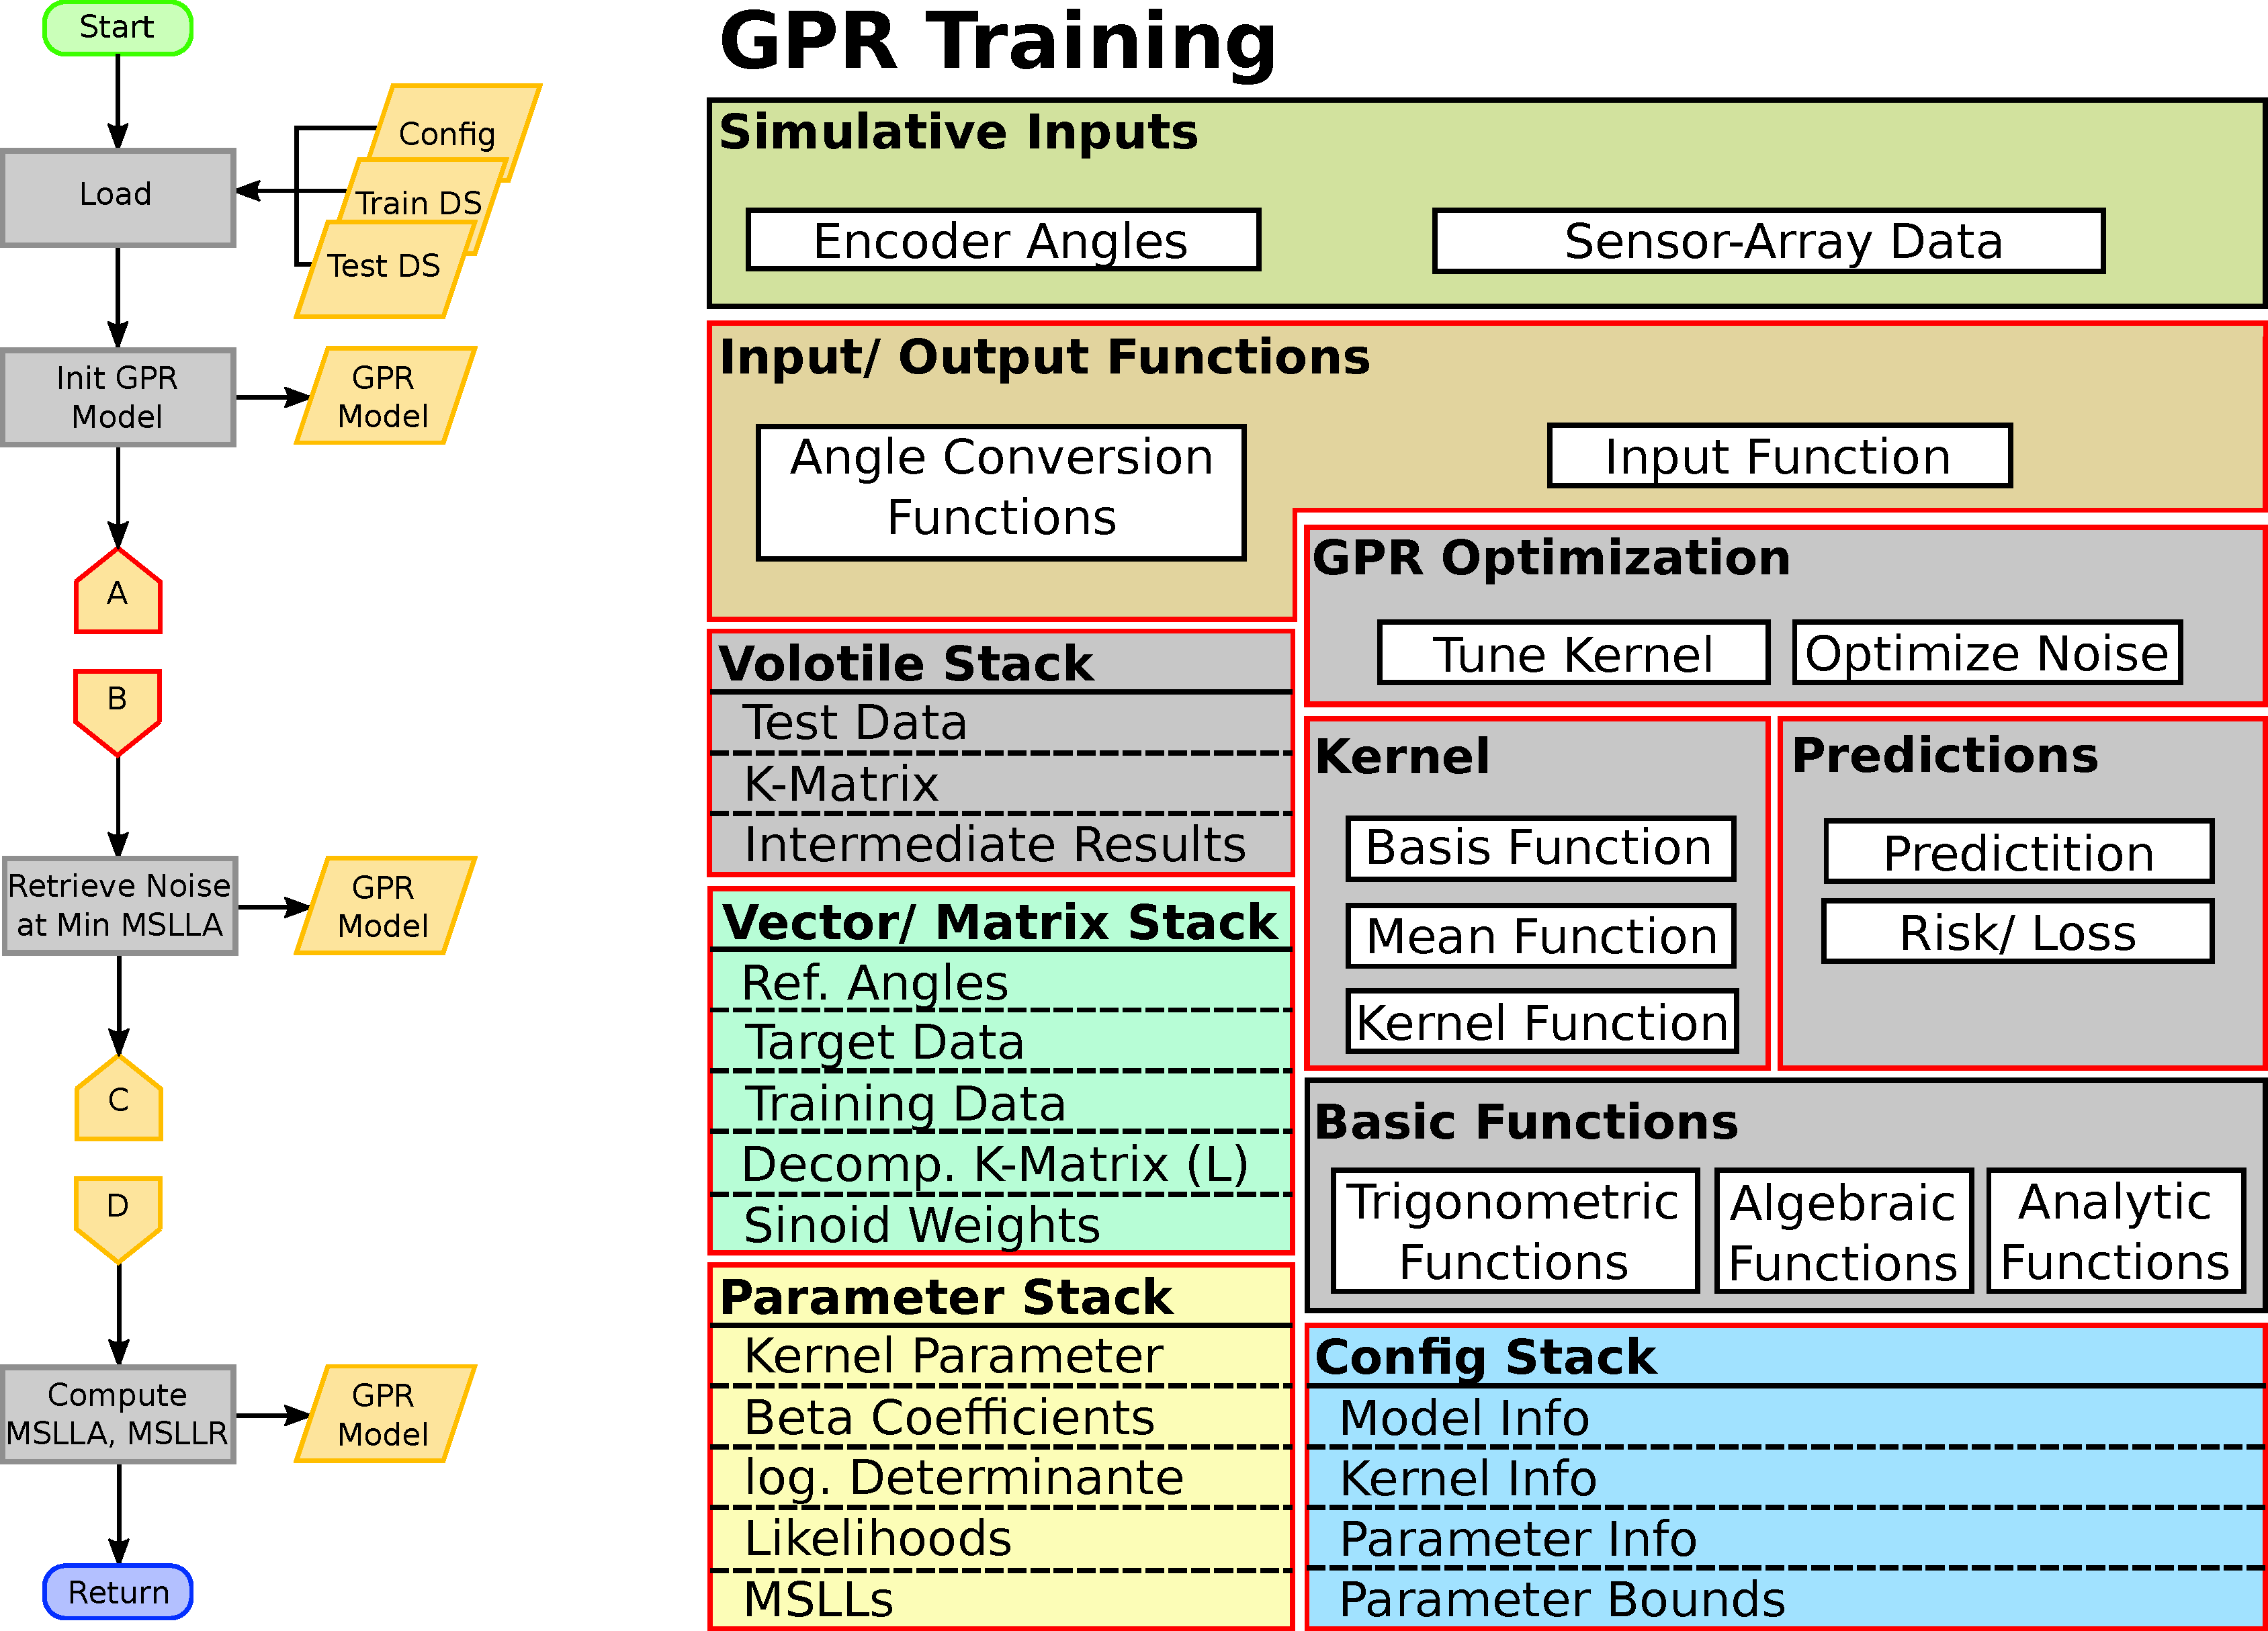
\includegraphics[width=.8\linewidth]{images/GPR_Trainingsphase-5}
	\end{overprint}
\end{figure}
\end{frame}
%%%%%%%%%%%%%%%%%%%%%%%%%%%%%%%%%%%%%%%%%%%%%%%%%%%%%%%%%%%%%%%%%%%%%%%%%%%%%%%%%%%%%%%%%%%%%%%%%%%%%%%%%%%%%%%%%%%%%%%%%%%%%%%%%%%%%%%%%
\begin{frame}
\frametitle{GPR-Verfahren}
\framesubtitle{GPR-Trainingsphase}
\textbf{Äußere Optimierung (Modell):}
\begin{columns}[c]
	\column{.45\textwidth}
	\begin{itemize}
		\item<2-> Bayes-Optimierung, Std.-Verfahren
		\item<2-> Improve-Per-$2^{nd}+$
		\item<3-> Anpassung üb. alle Winkel
		\item<4-> Vorgabe von $\sigma_n^2=konst.$
		\item<5-> Durchlaufzahl entscheidend
		\item<6-> Modellsuche
	\end{itemize}
	\begin{block}{Min.-Kriterium}<7->
		\scalebox{.7}{\parbox{\hsize}{%
		\begin{align*}%
			\sigma_n^2|\mathcal{D},\alpha_* &= \arg\min MSLLA(\sigma_n^2|\mathcal{D},\alpha_*) \\%
			SLLA &= 0,5\cdot\bigg(\log(2\pi\sigma_*^2) + \frac{(\alpha - \alpha_*)^2}{\sigma_*^2}\bigg) \\%
			\sigma_*^2 &= \sigma_n^2 + V_*%
		\end{align*}%
		}}
	\end{block}

	\column{.5\textwidth}
	\begin{figure}
		\begin{overprint}
			\onslide<1-7>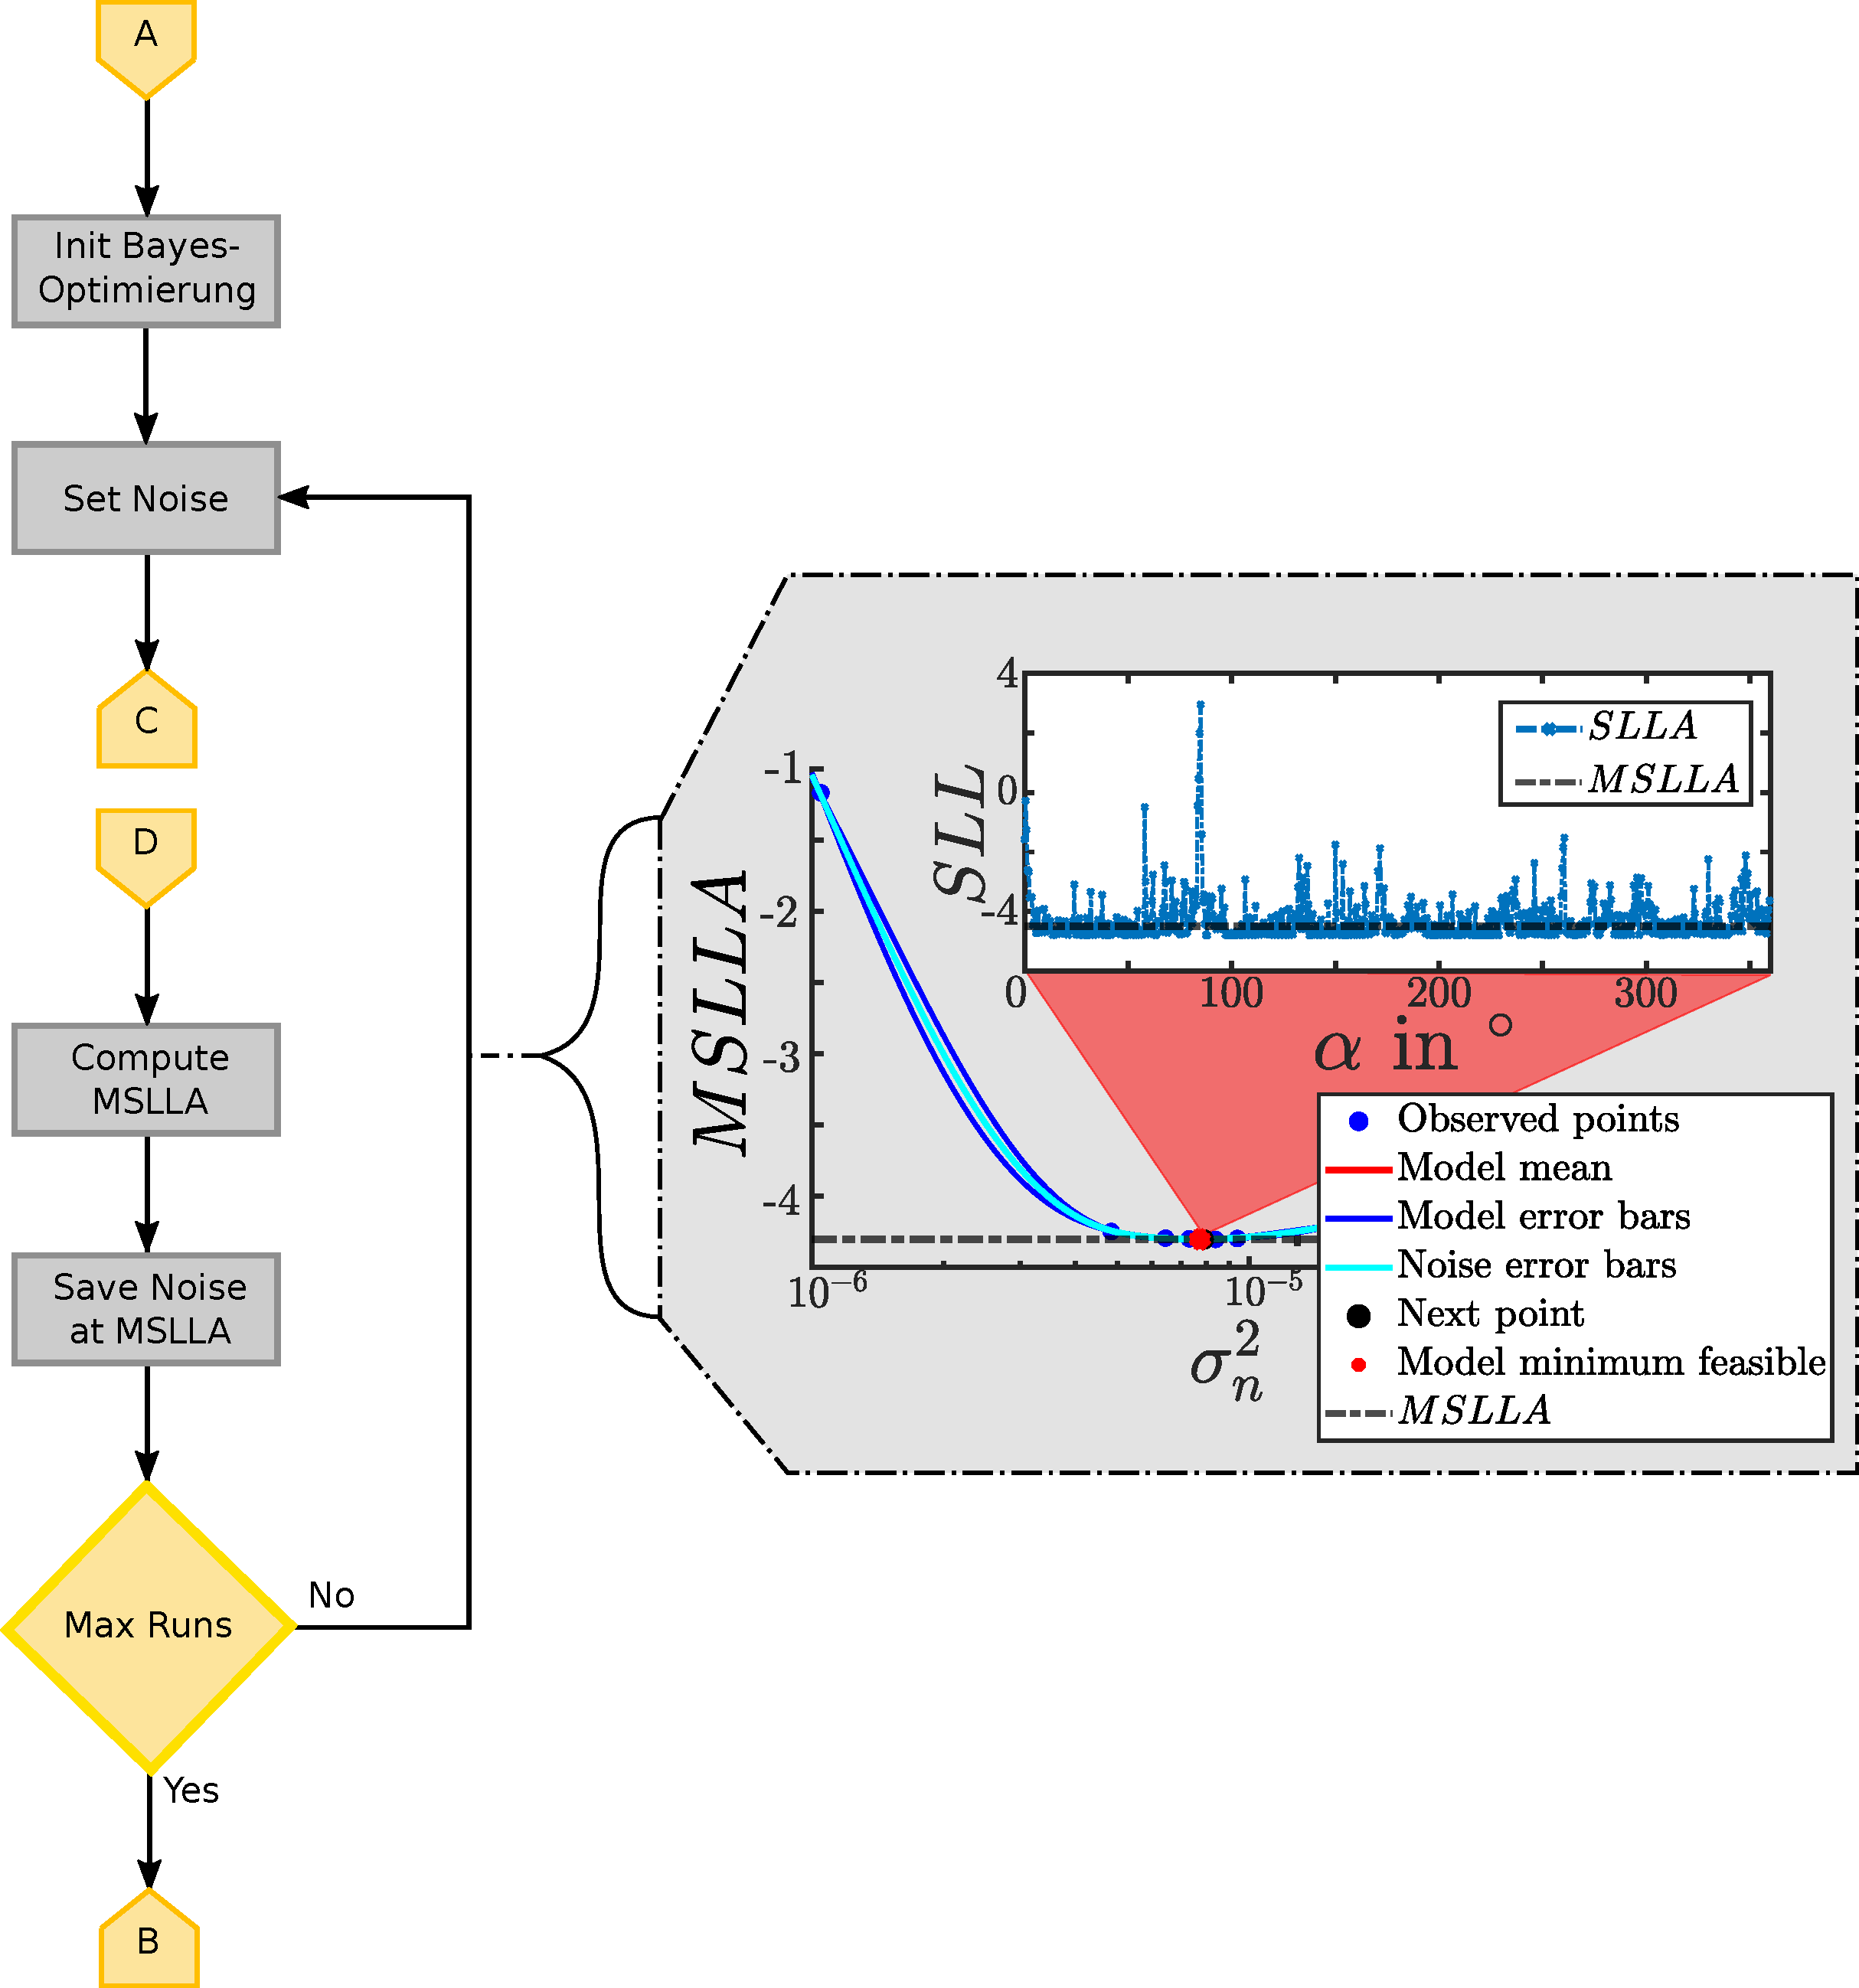
\includegraphics[width=\linewidth]{images/Noise_Optimization}
			\onslide<8>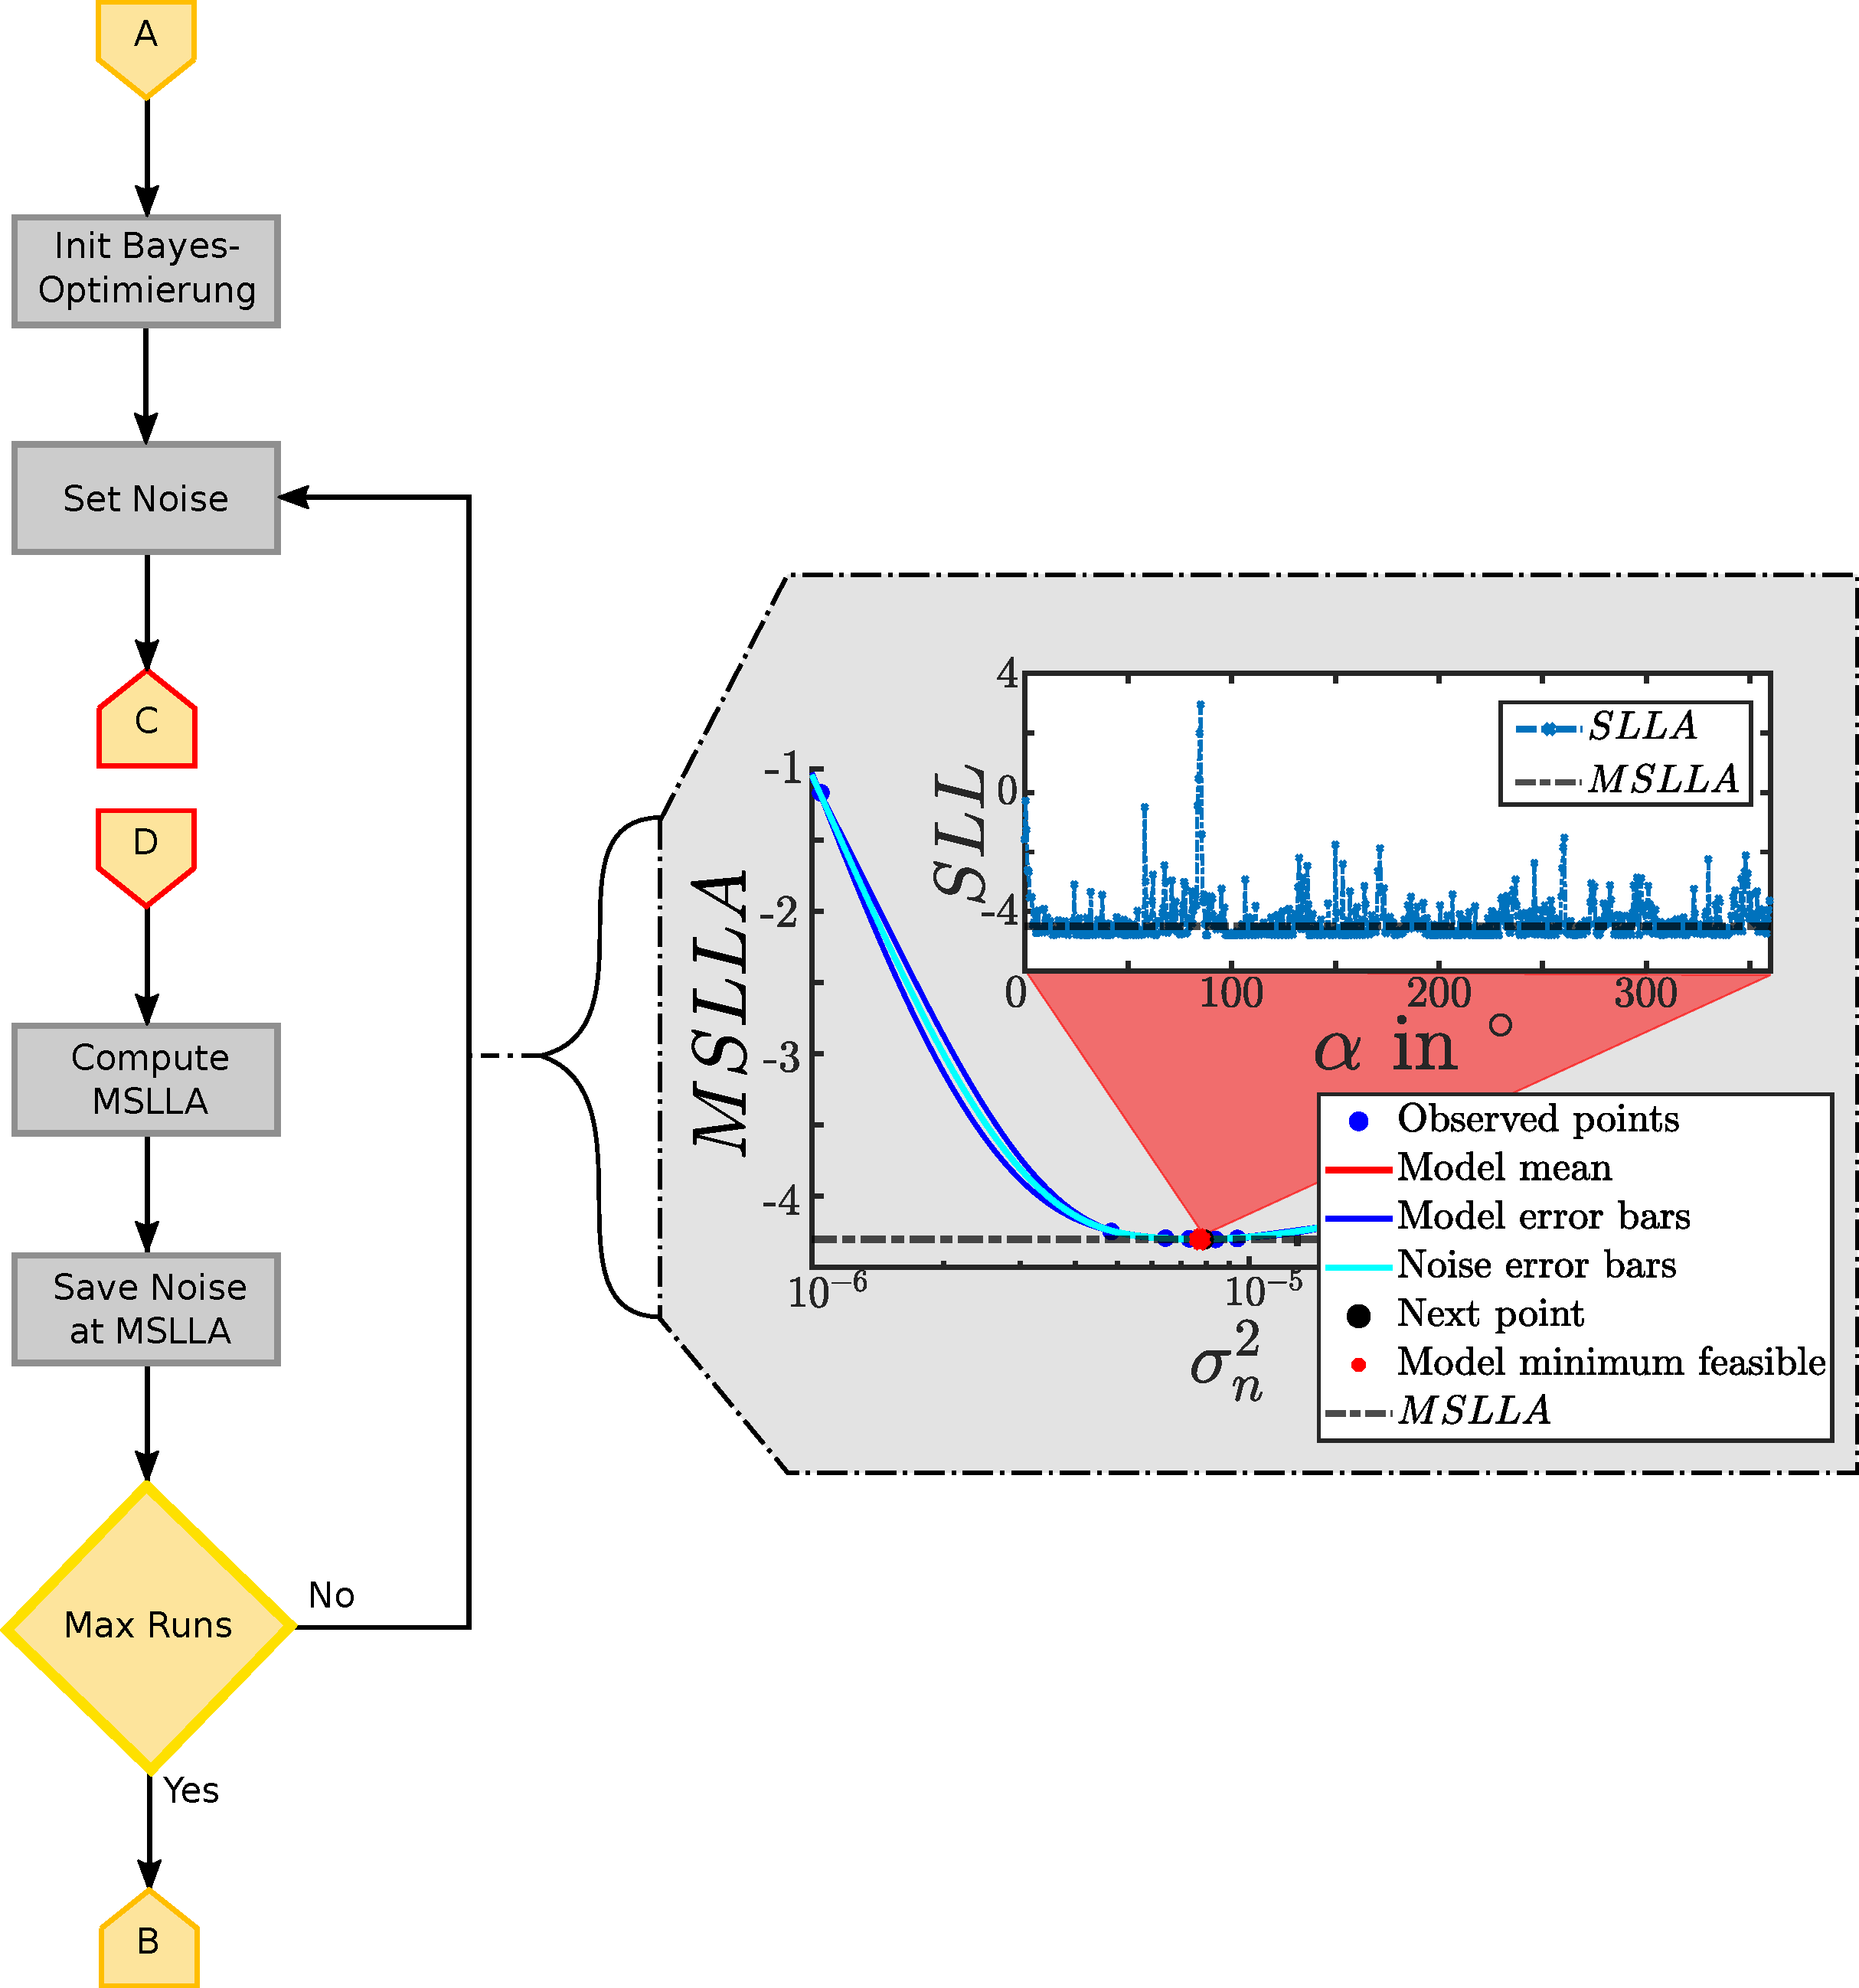
\includegraphics[width=\linewidth]{images/Noise_Optimization-1}
		\end{overprint}
	\end{figure}
\end{columns}
\end{frame}
%%%%%%%%%%%%%%%%%%%%%%%%%%%%%%%%%%%%%%%%%%%%%%%%%%%%%%%%%%%%%%%%%%%%%%%%%%%%%%%%%%%%%%%%%%%%%%%%%%%%%%%%%%%%%%%%%%%%%%%%%%%%%%%%%%%%%%%%%
\begin{frame}
\frametitle{GPR-Verfahren}
\framesubtitle{GPR-Trainingsphase}
\textbf{Innere Optimierung (Fit):}
\begin{columns}[c]
	\column{.45\textwidth}
	\begin{itemize}
		\item<2-> fmincon, Std.-Verfahren
		\item<2-> SQP, klein- bis mittlere Probleme
		\item<3-> Fit auf Trainingsdaten
		\item<4-> Teilreinitialisierung
		\item<5-> Bounds entscheidend
		\item<6-> Best-Fit-Suche
	\end{itemize}
	\begin{block}{Min.-Kriterium}<7->
	\scalebox{.7}{\parbox{\hsize}{%
		\begin{align*}%
			\sigma_l,\sigma_f^2|\sigma_n^2 & = \arg\min\tilde{R}_{\mathcal{L}}(\sigma_l,\sigma_f^2|\sigma_n^2) \\
			\tilde{R}_{\mathcal{L}}(\sigma_l,\sigma_f^2|\sigma_n^2) &= -(\log p(y_{cos}|X_{cos},\sigma_l,\sigma_f^2,\sigma_n^2) + \\
																	& \log p(y_{sin}|X_{sin},\sigma_l,\sigma_f^2,\sigma_n^2))
		\end{align*}%
	}}
	\end{block}			

	\column{.5\textwidth}
	\begin{figure}
		\begin{overprint}
			\onslide<1->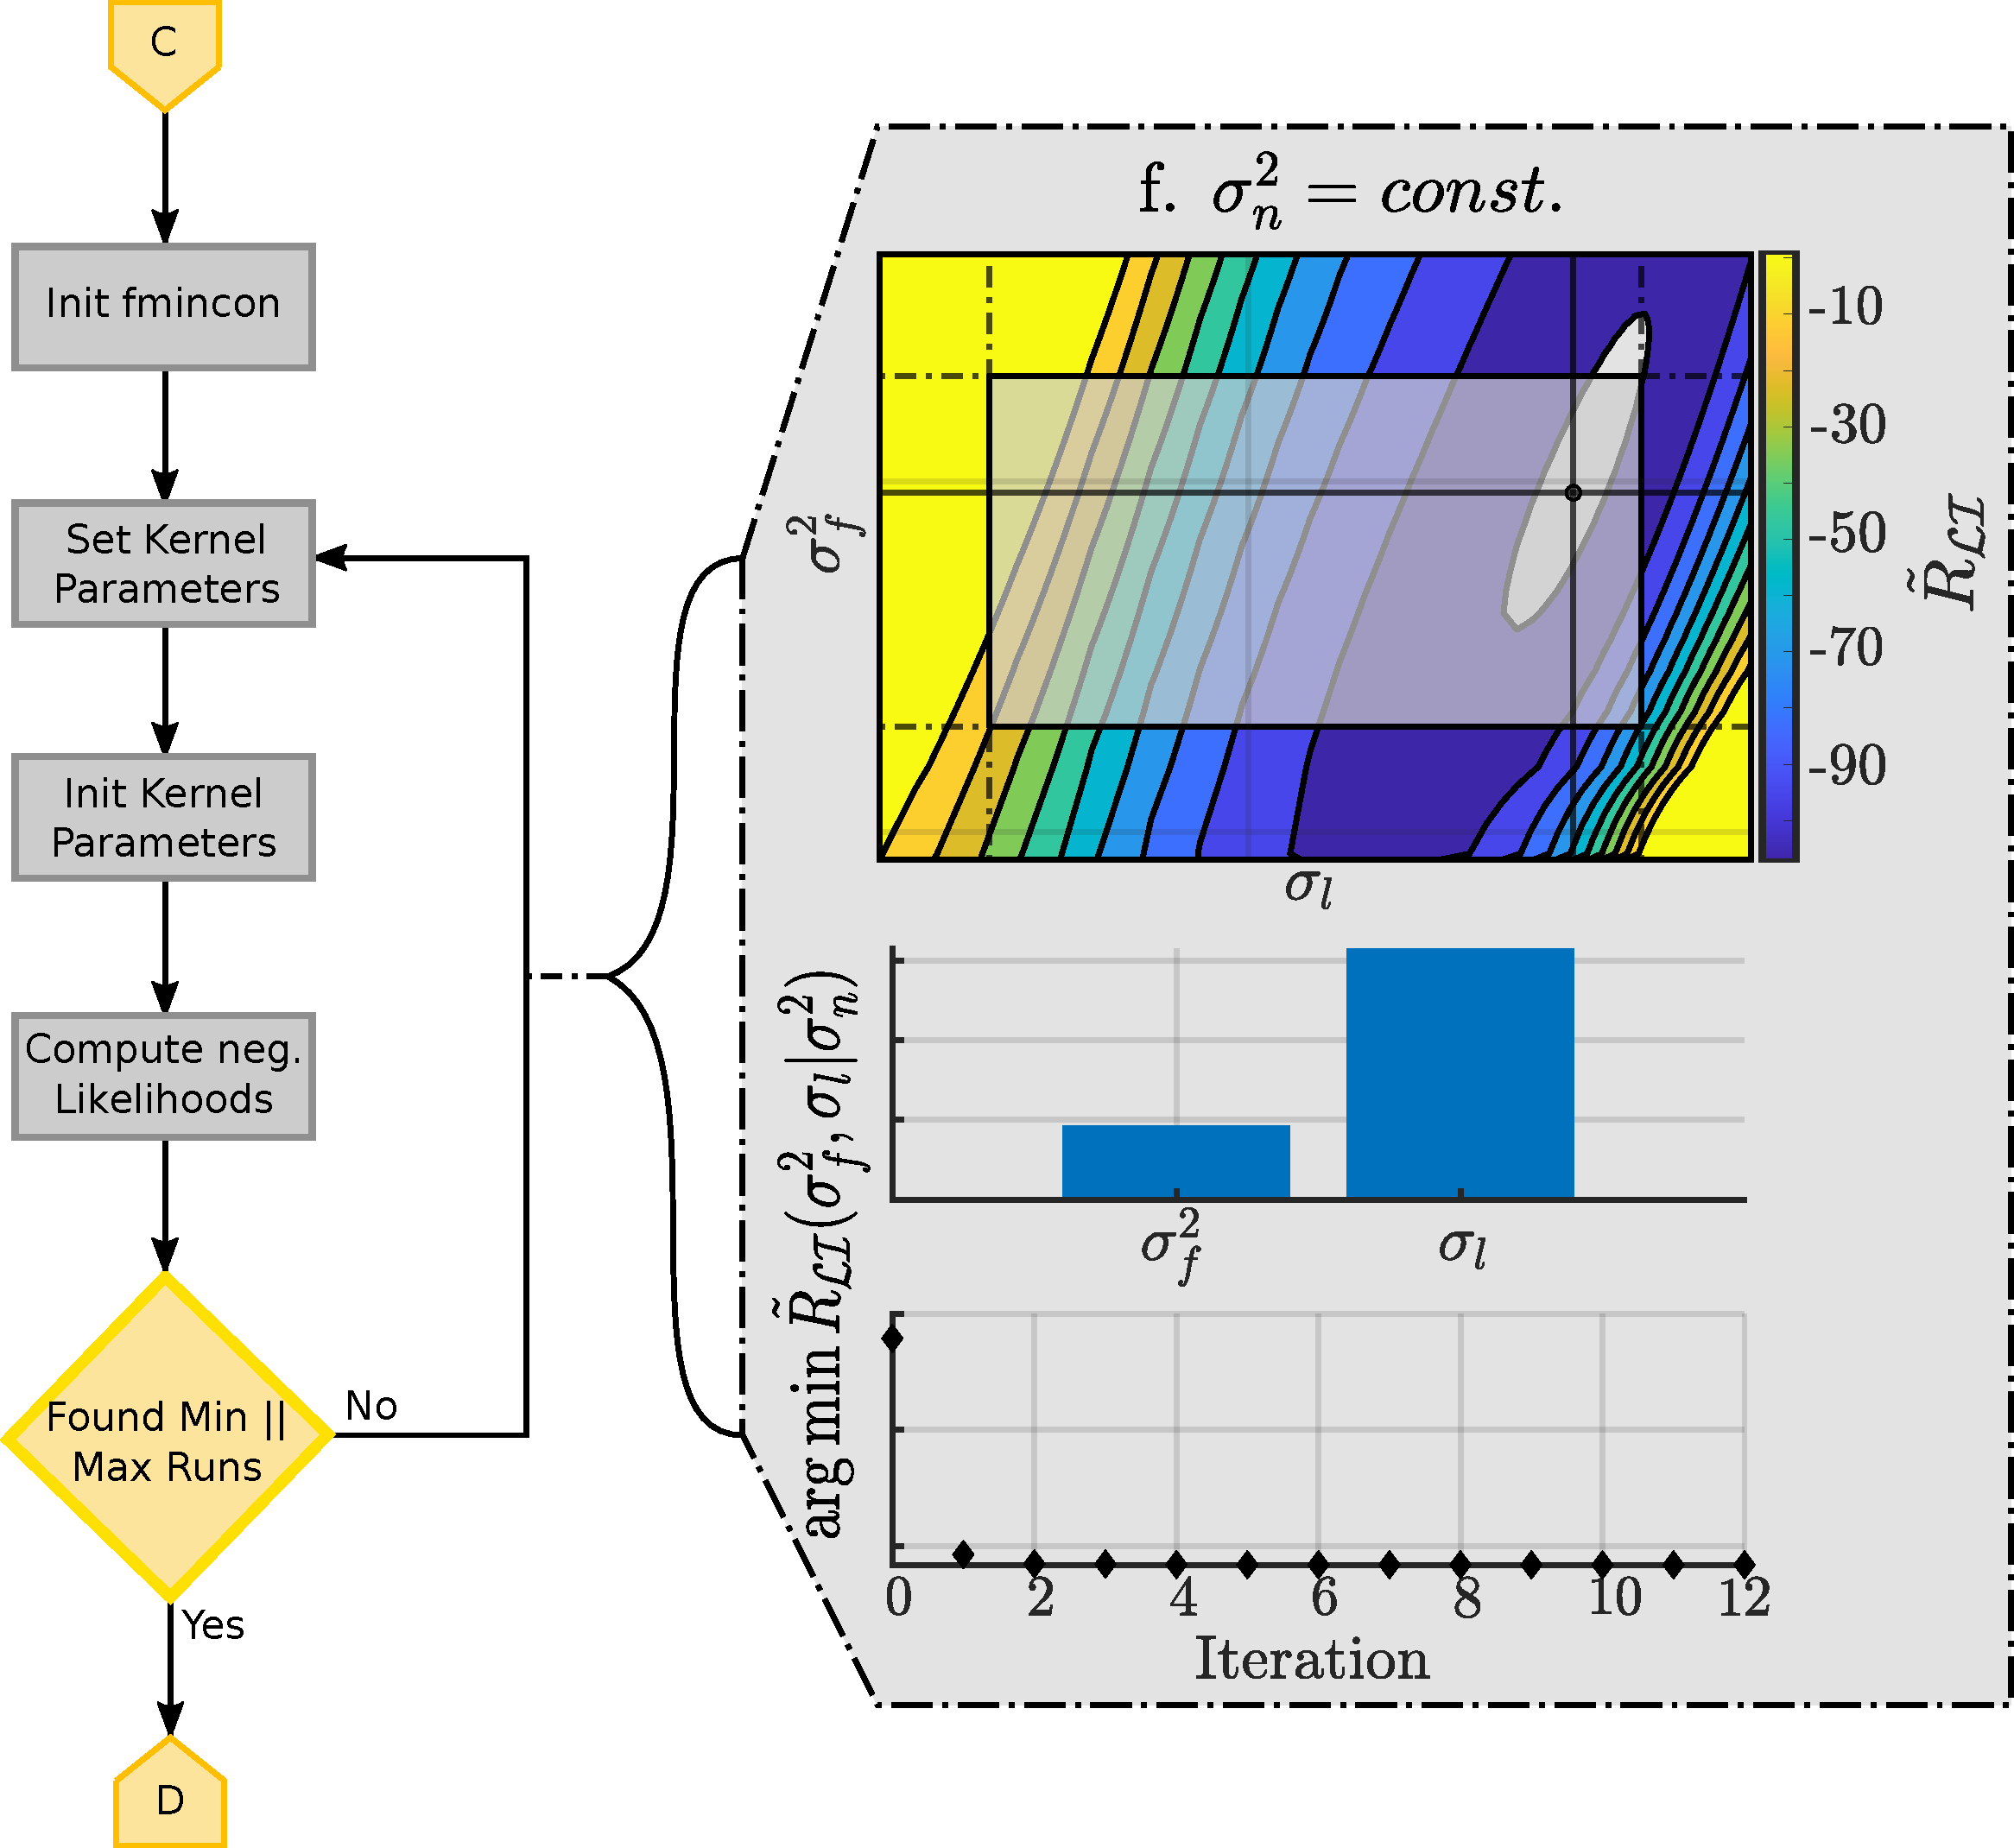
\includegraphics[width=\linewidth]{images/Kernel_Tuning}
		\end{overprint}
	\end{figure}
\end{columns}
\end{frame}
%%%%%%%%%%%%%%%%%%%%%%%%%%%%%%%%%%%%%%%%%%%%%%%%%%%%%%%%%%%%%%%%%%%%%%%%%%%%%%%%%%%%%%%%%%%%%%%%%%%%%%%%%%%%%%%%%%%%%%%%%%%%%%%%%%%%%%%%%
\begin{frame}
\frametitle{GPR-Verfahren}
\framesubtitle{GPR-Trainingsphase}
\begin{figure}
	\begin{overprint}
		\onslide<1>\centering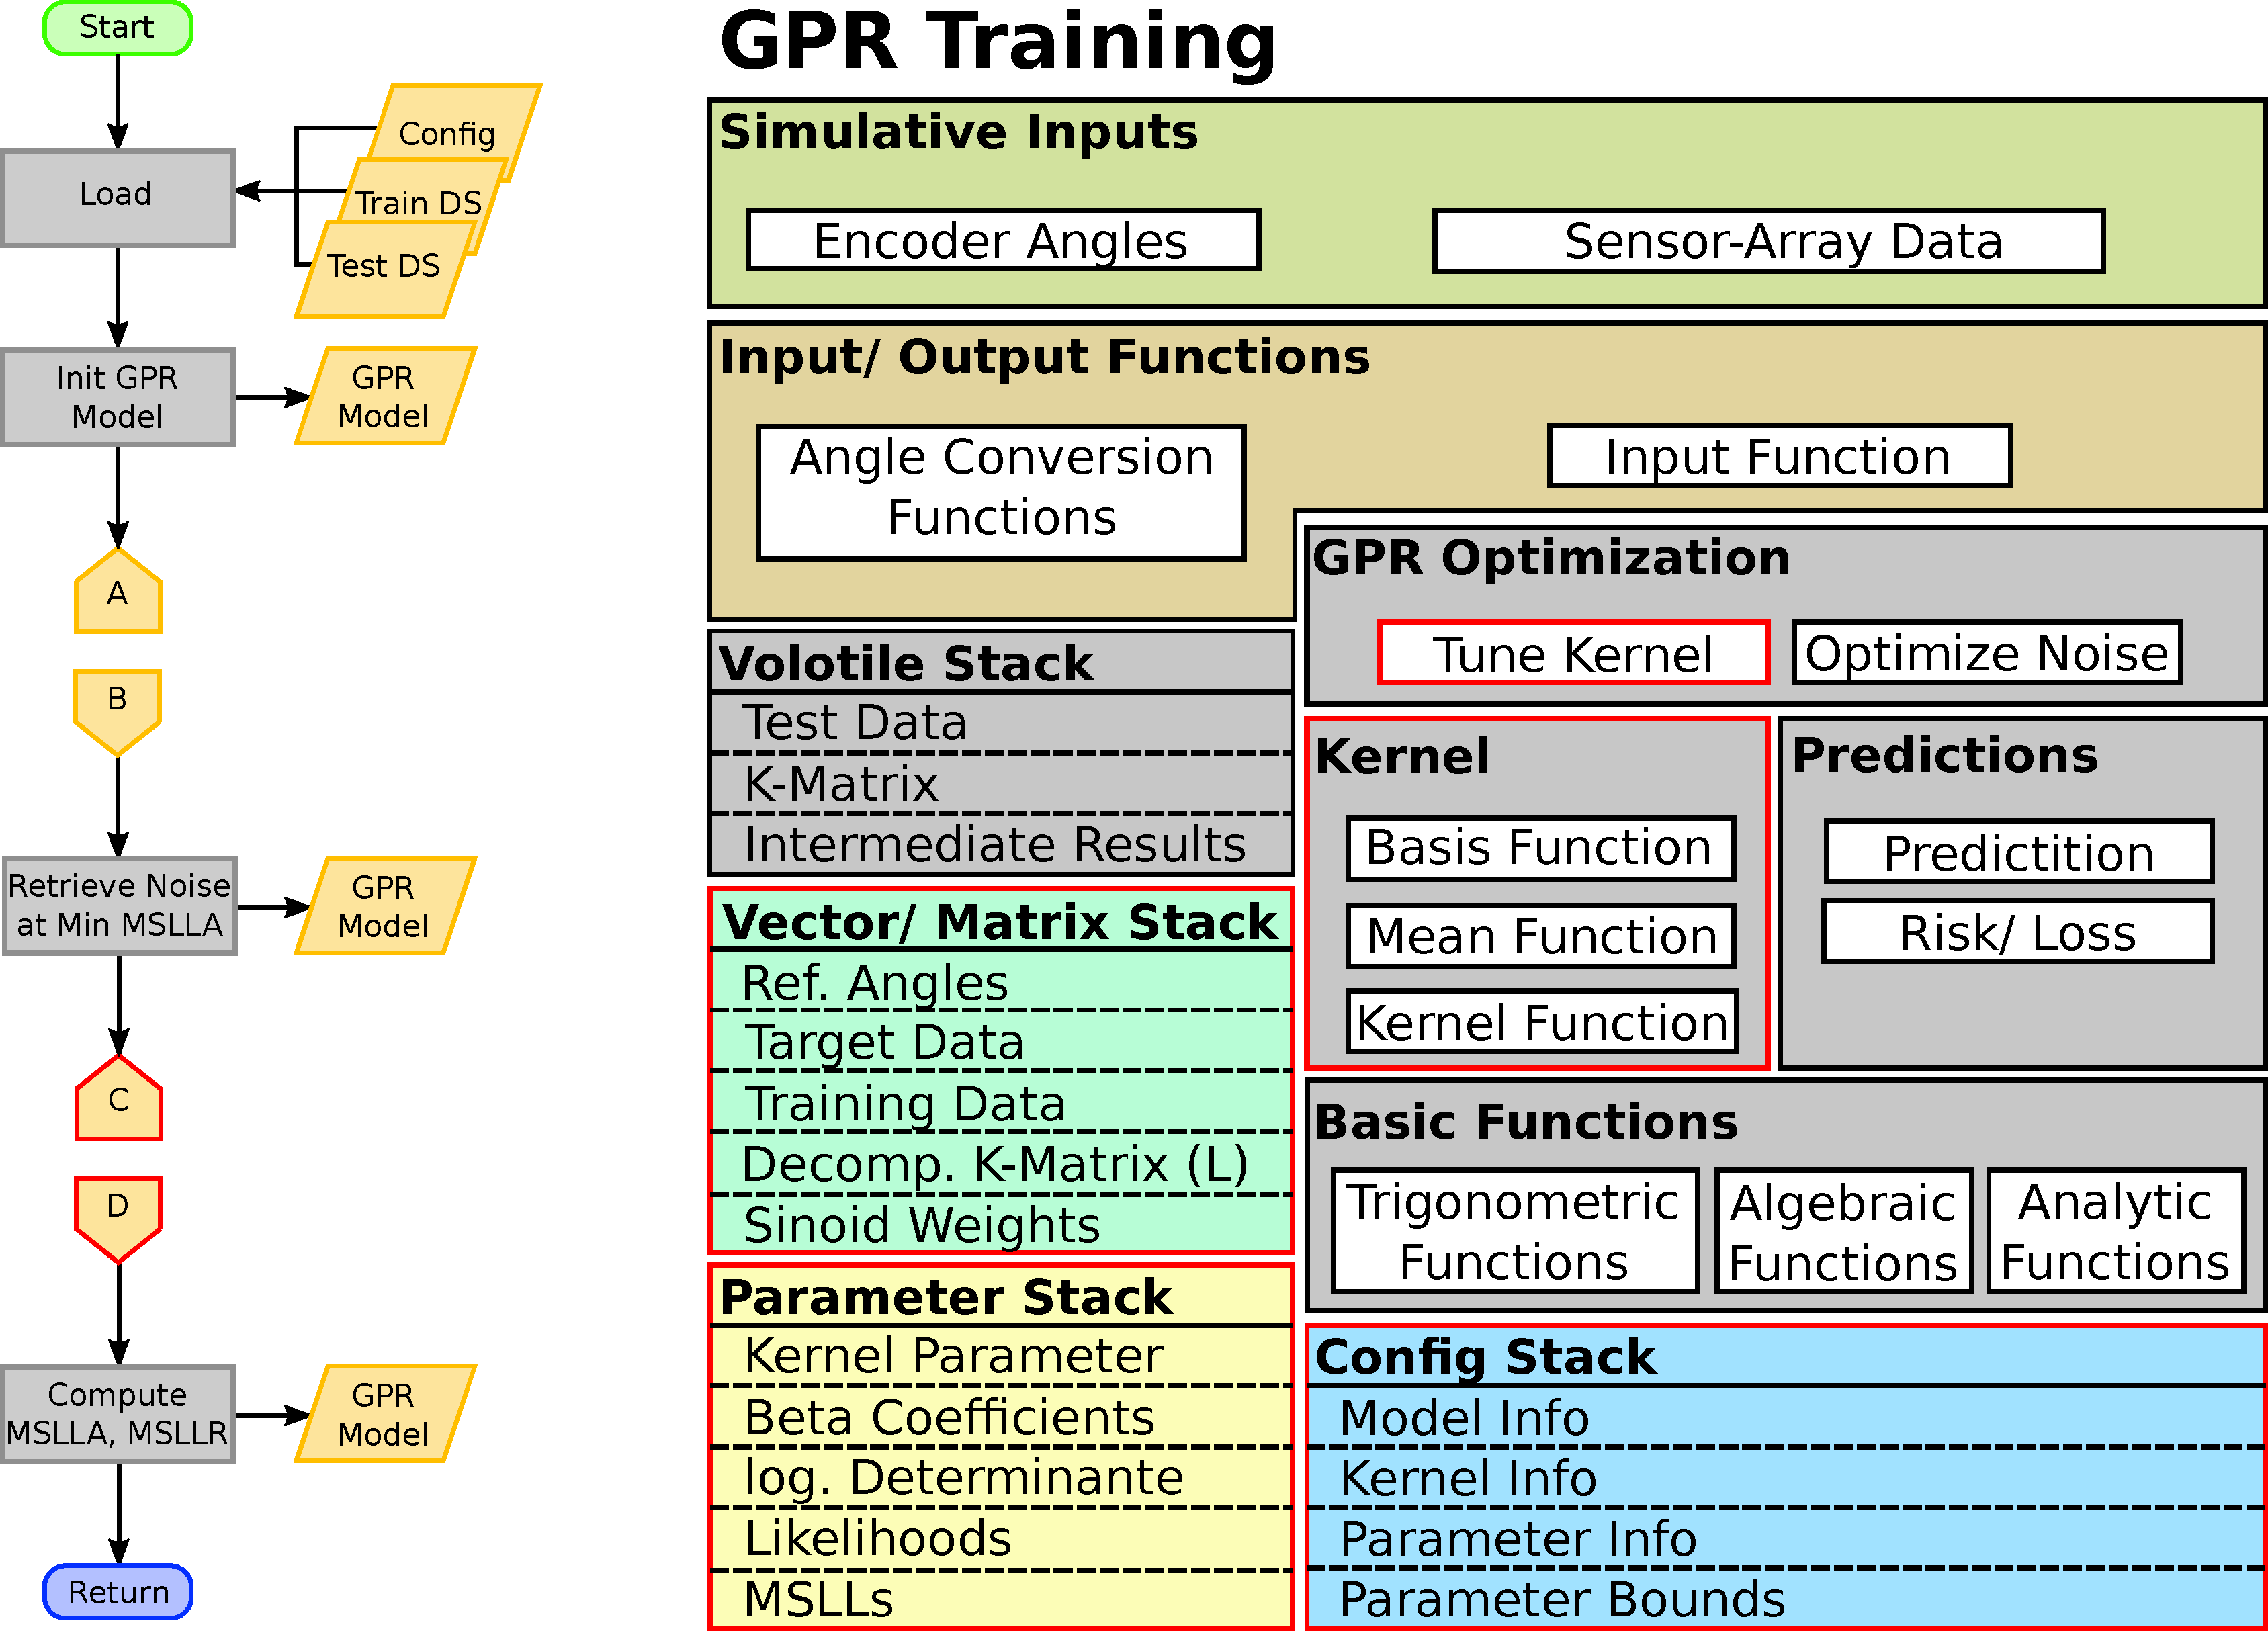
\includegraphics[width=.8\linewidth]{images/GPR_Trainingsphase-6}
	\end{overprint}
\end{figure}
\end{frame}
%%%%%%%%%%%%%%%%%%%%%%%%%%%%%%%%%%%%%%%%%%%%%%%%%%%%%%%%%%%%%%%%%%%%%%%%%%%%%%%%%%%%%%%%%%%%%%%%%%%%%%%%%%%%%%%%%%%%%%%%%%%%%%%%%%%%%%%%%
\begin{frame}
\frametitle{GPR-Verfahren}
\framesubtitle{GPR-Trainingsphase}
\begin{figure}
	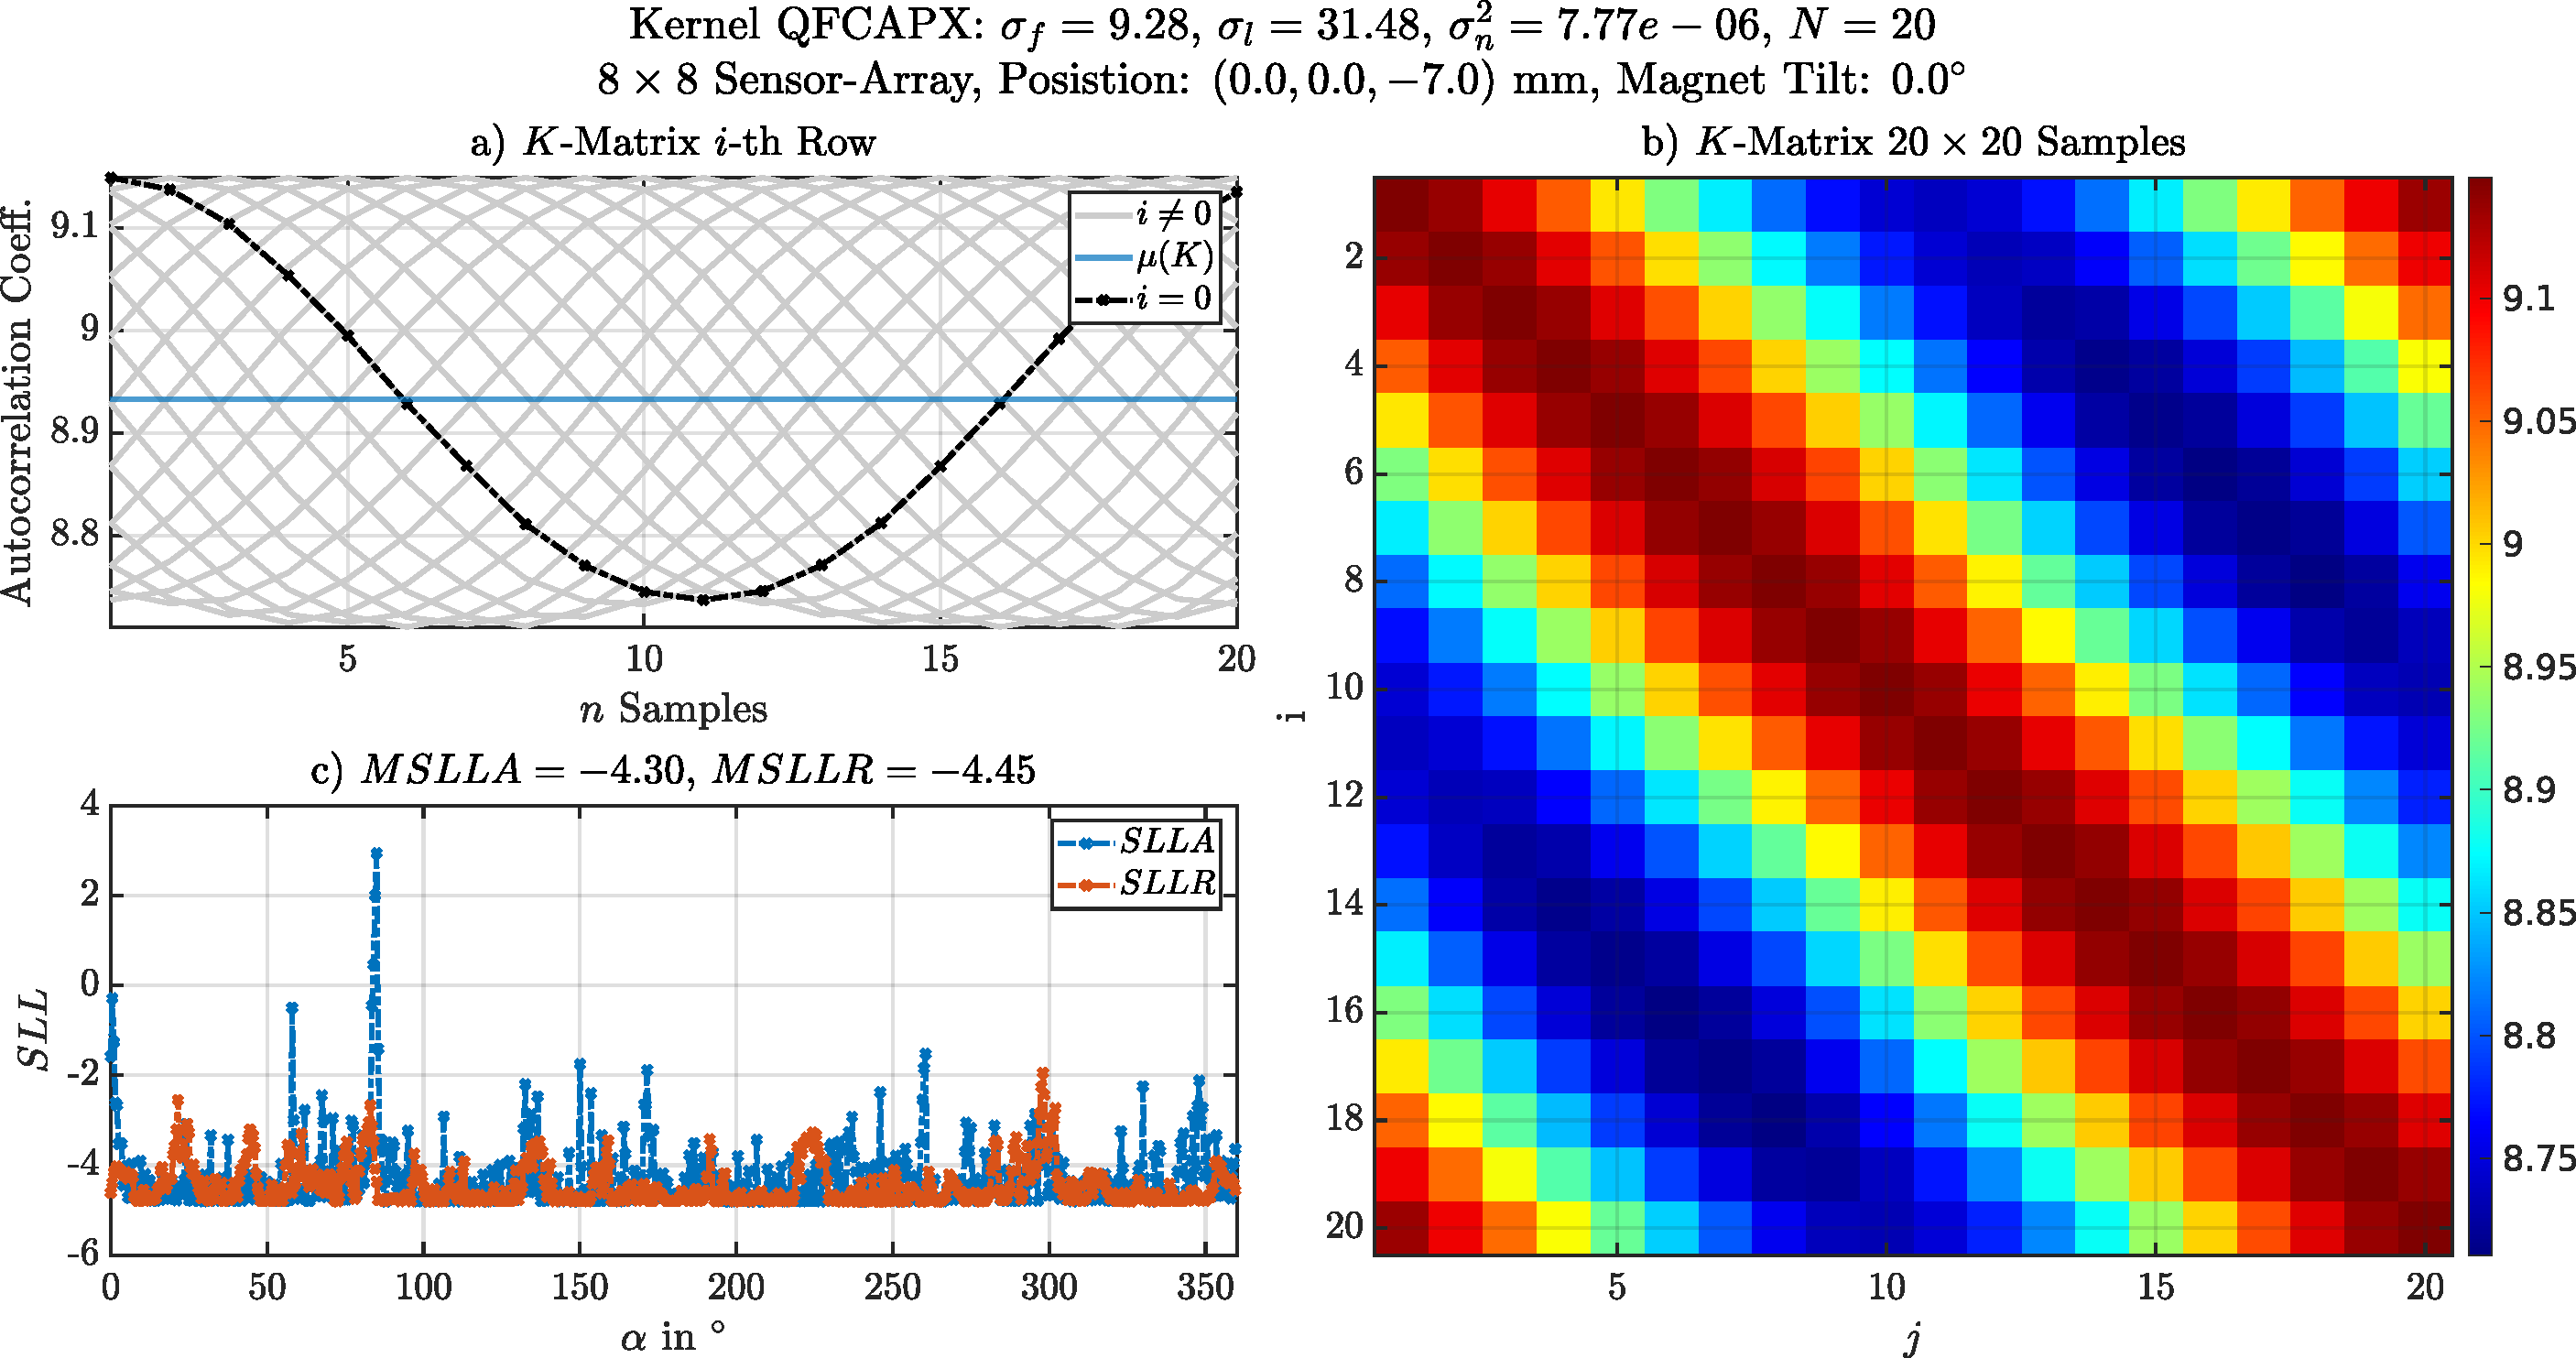
\includegraphics[width=.9\linewidth]{images/K-Matrix}
\end{figure}
\begin{columns}[c]
	\column{.45\textwidth}
	\begin{itemize}
		\item<1-> Fit abhängig von Auflösung
		\item<2-> Ausgleich $\mu(K)$, mittige Platzierung
	\end{itemize}

	\column{.45\textwidth}
	\begin{itemize}
		\item<3-> SLLA nur in Trainingsphase
		\item<4-> SLLR in beiden Phasen
	\end{itemize}
\end{columns}
\end{frame}
%%%%%%%%%%%%%%%%%%%%%%%%%%%%%%%%%%%%%%%%%%%%%%%%%%%%%%%%%%%%%%%%%%%%%%%%%%%%%%%%%%%%%%%%%%%%%%%%%%%%%%%%%%%%%%%%%%%%%%%%%%%%%%%%%%%%%%%%%
\subsection{GPR-Arbeitsphase}
\begin{frame}
\frametitle{GPR-Verfahren}
\framesubtitle{GPR-Arbeitsphase}
\begin{columns}[c]
	\column{.45\textwidth}
	\begin{itemize}
		\item<2-> Umlegen d. Ausrichtung
		\item<3-> Min. Parametrierung
		\item<4-> Freie Ressourcen
		\item<5-> Vorhersage Sinoide
		\item<6-> Winkel, Radius abgeleitet
		\item<7-> Mehrere Qualitätskriterien
		\begin{itemize}
			\item<7-> Std.-Abweichung
			\item<8-> Konfidenzintervall Winkel
			\item<8-> Konfidenzintervall Radius
			\item<9-> Modellanpassung Radius
		\end{itemize}
	\end{itemize}
	\column{.55\textwidth}
	\begin{figure}
		\onslide<1->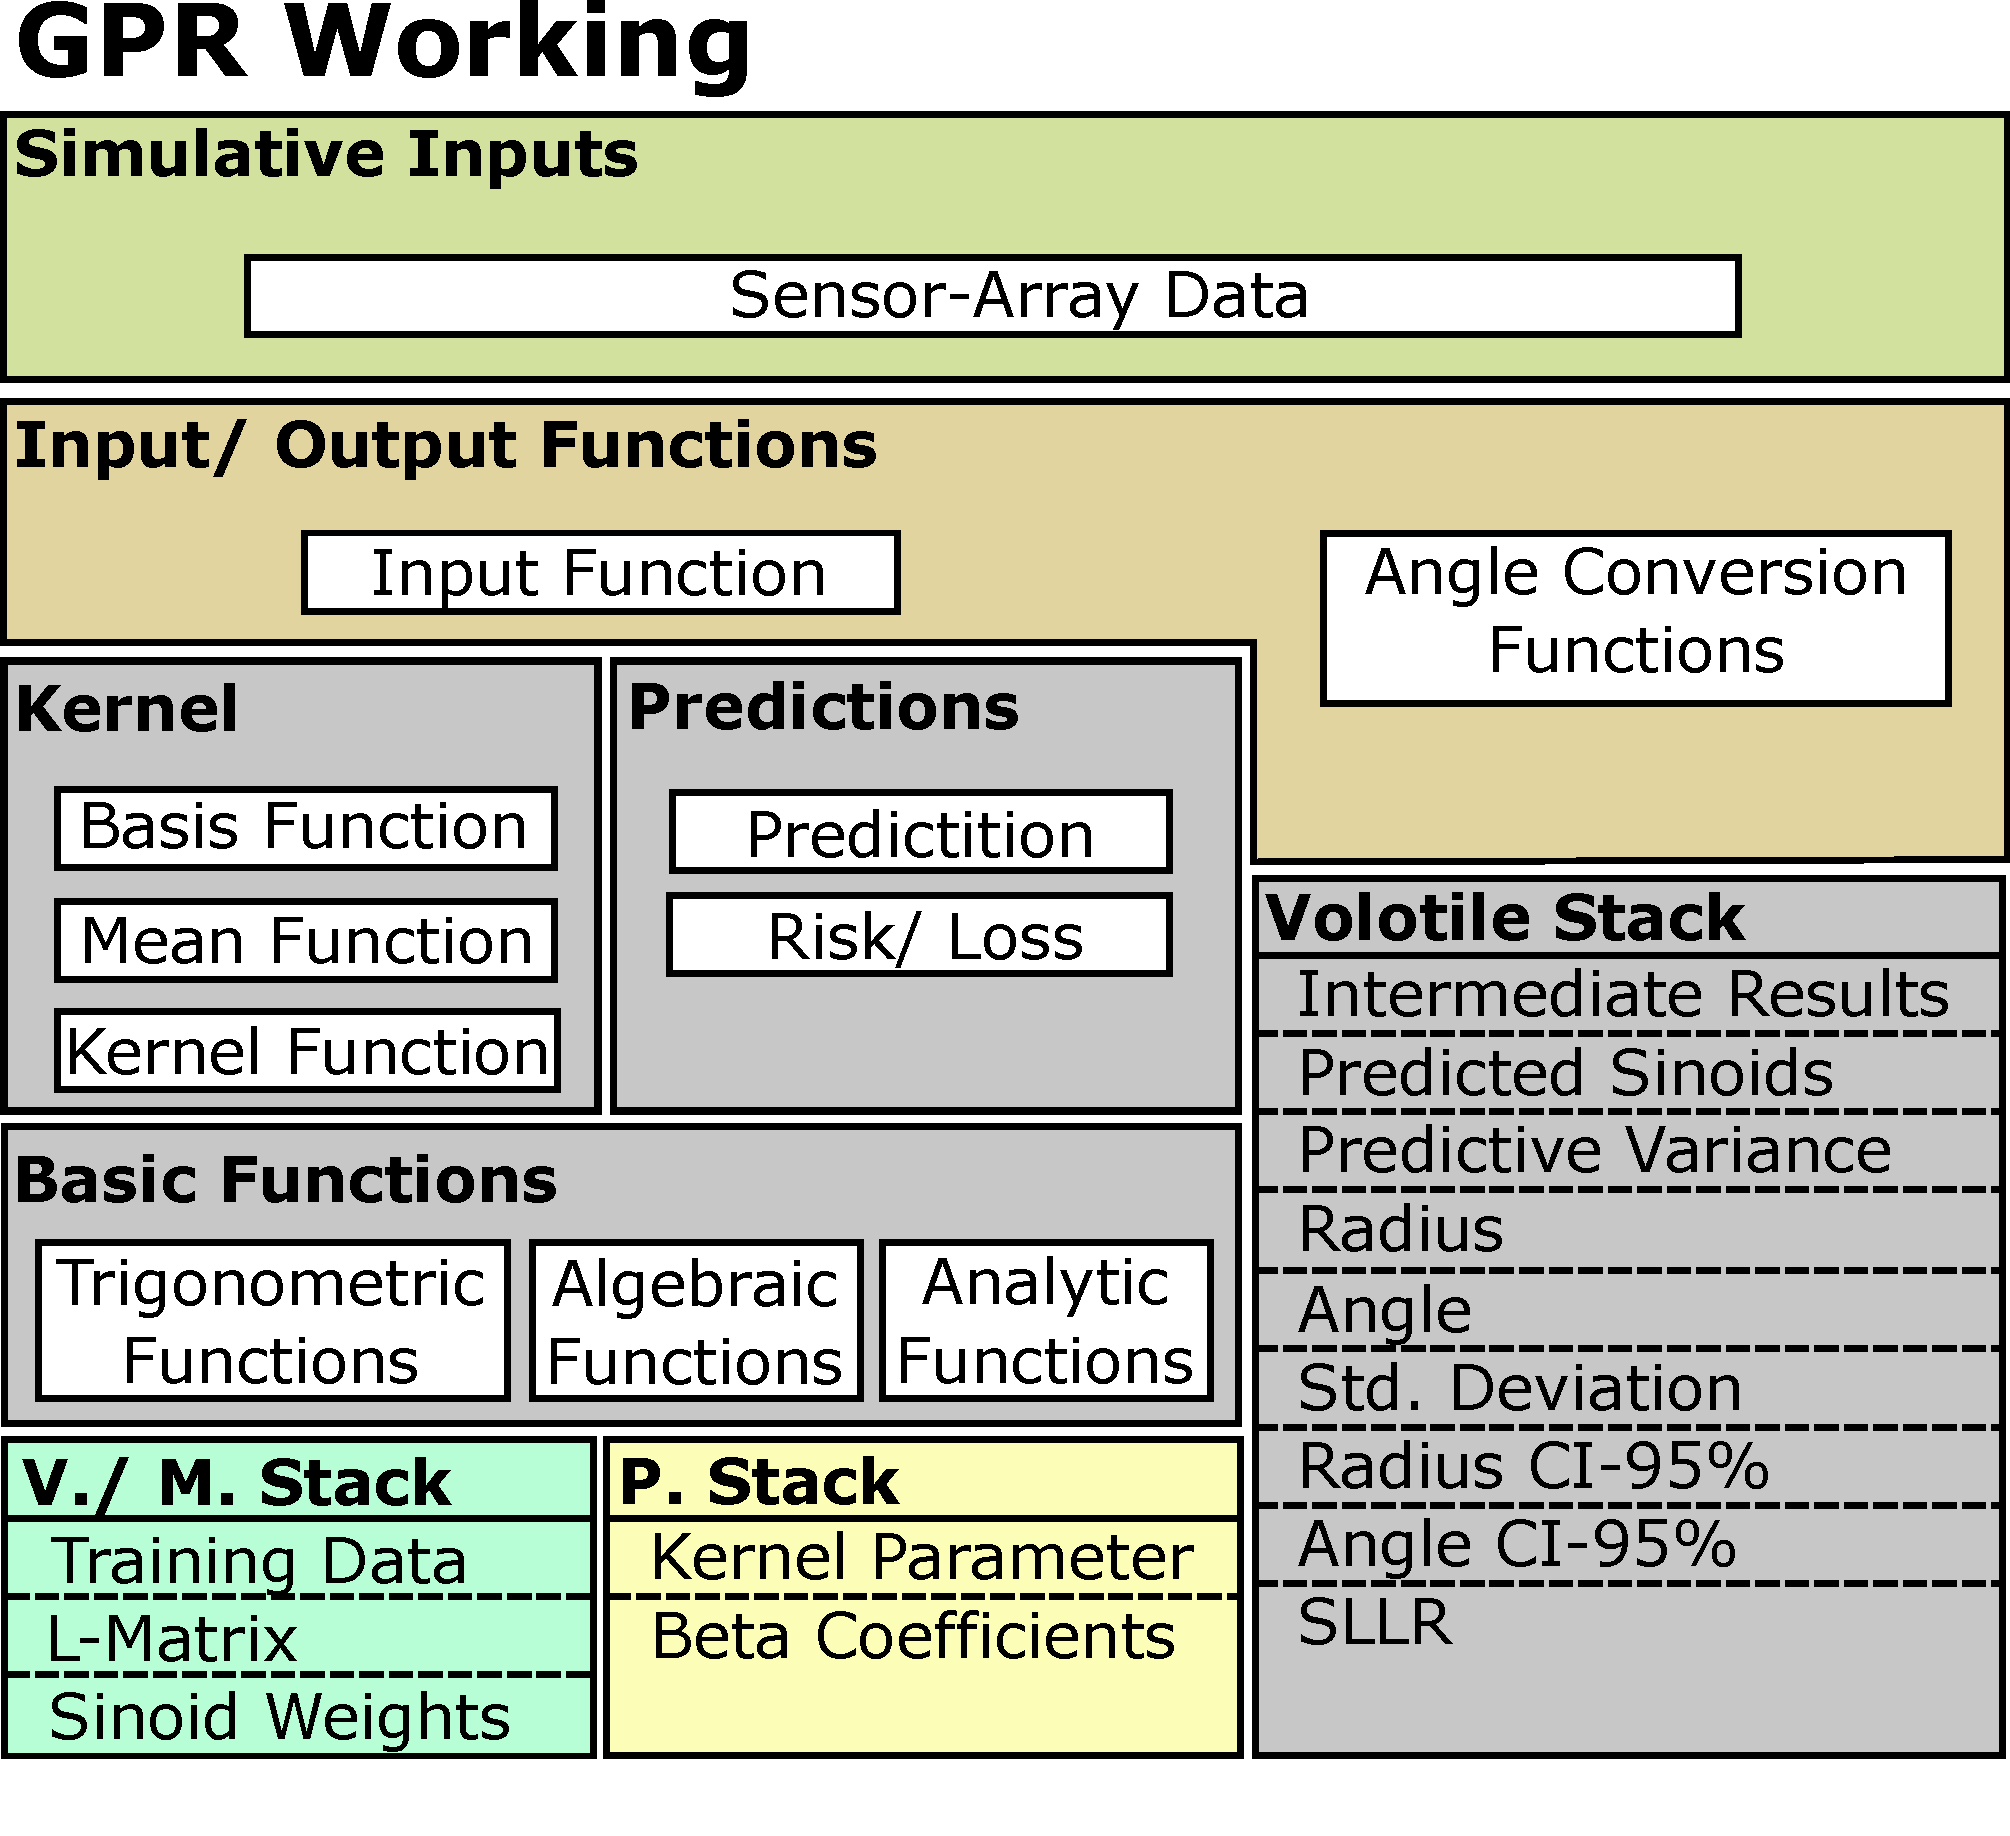
\includegraphics[width=\linewidth]{images/Blockschema_Workphase}
	\end{figure}
\end{columns}
\end{frame}
%%%%%%%%%%%%%%%%%%%%%%%%%%%%%%%%%%%%%%%%%%%%%%%%%%%%%%%%%%%%%%%%%%%%%%%%%%%%%%%%%%%%%%%%%%%%%%%%%%%%%%%%%%%%%%%%%%%%%%%%%%%%%%%%%%%%%%%%%
\begin{frame}
\frametitle{GPR-Verfahren}
\framesubtitle{GPR-Arbeitsphase}
\begin{figure}
	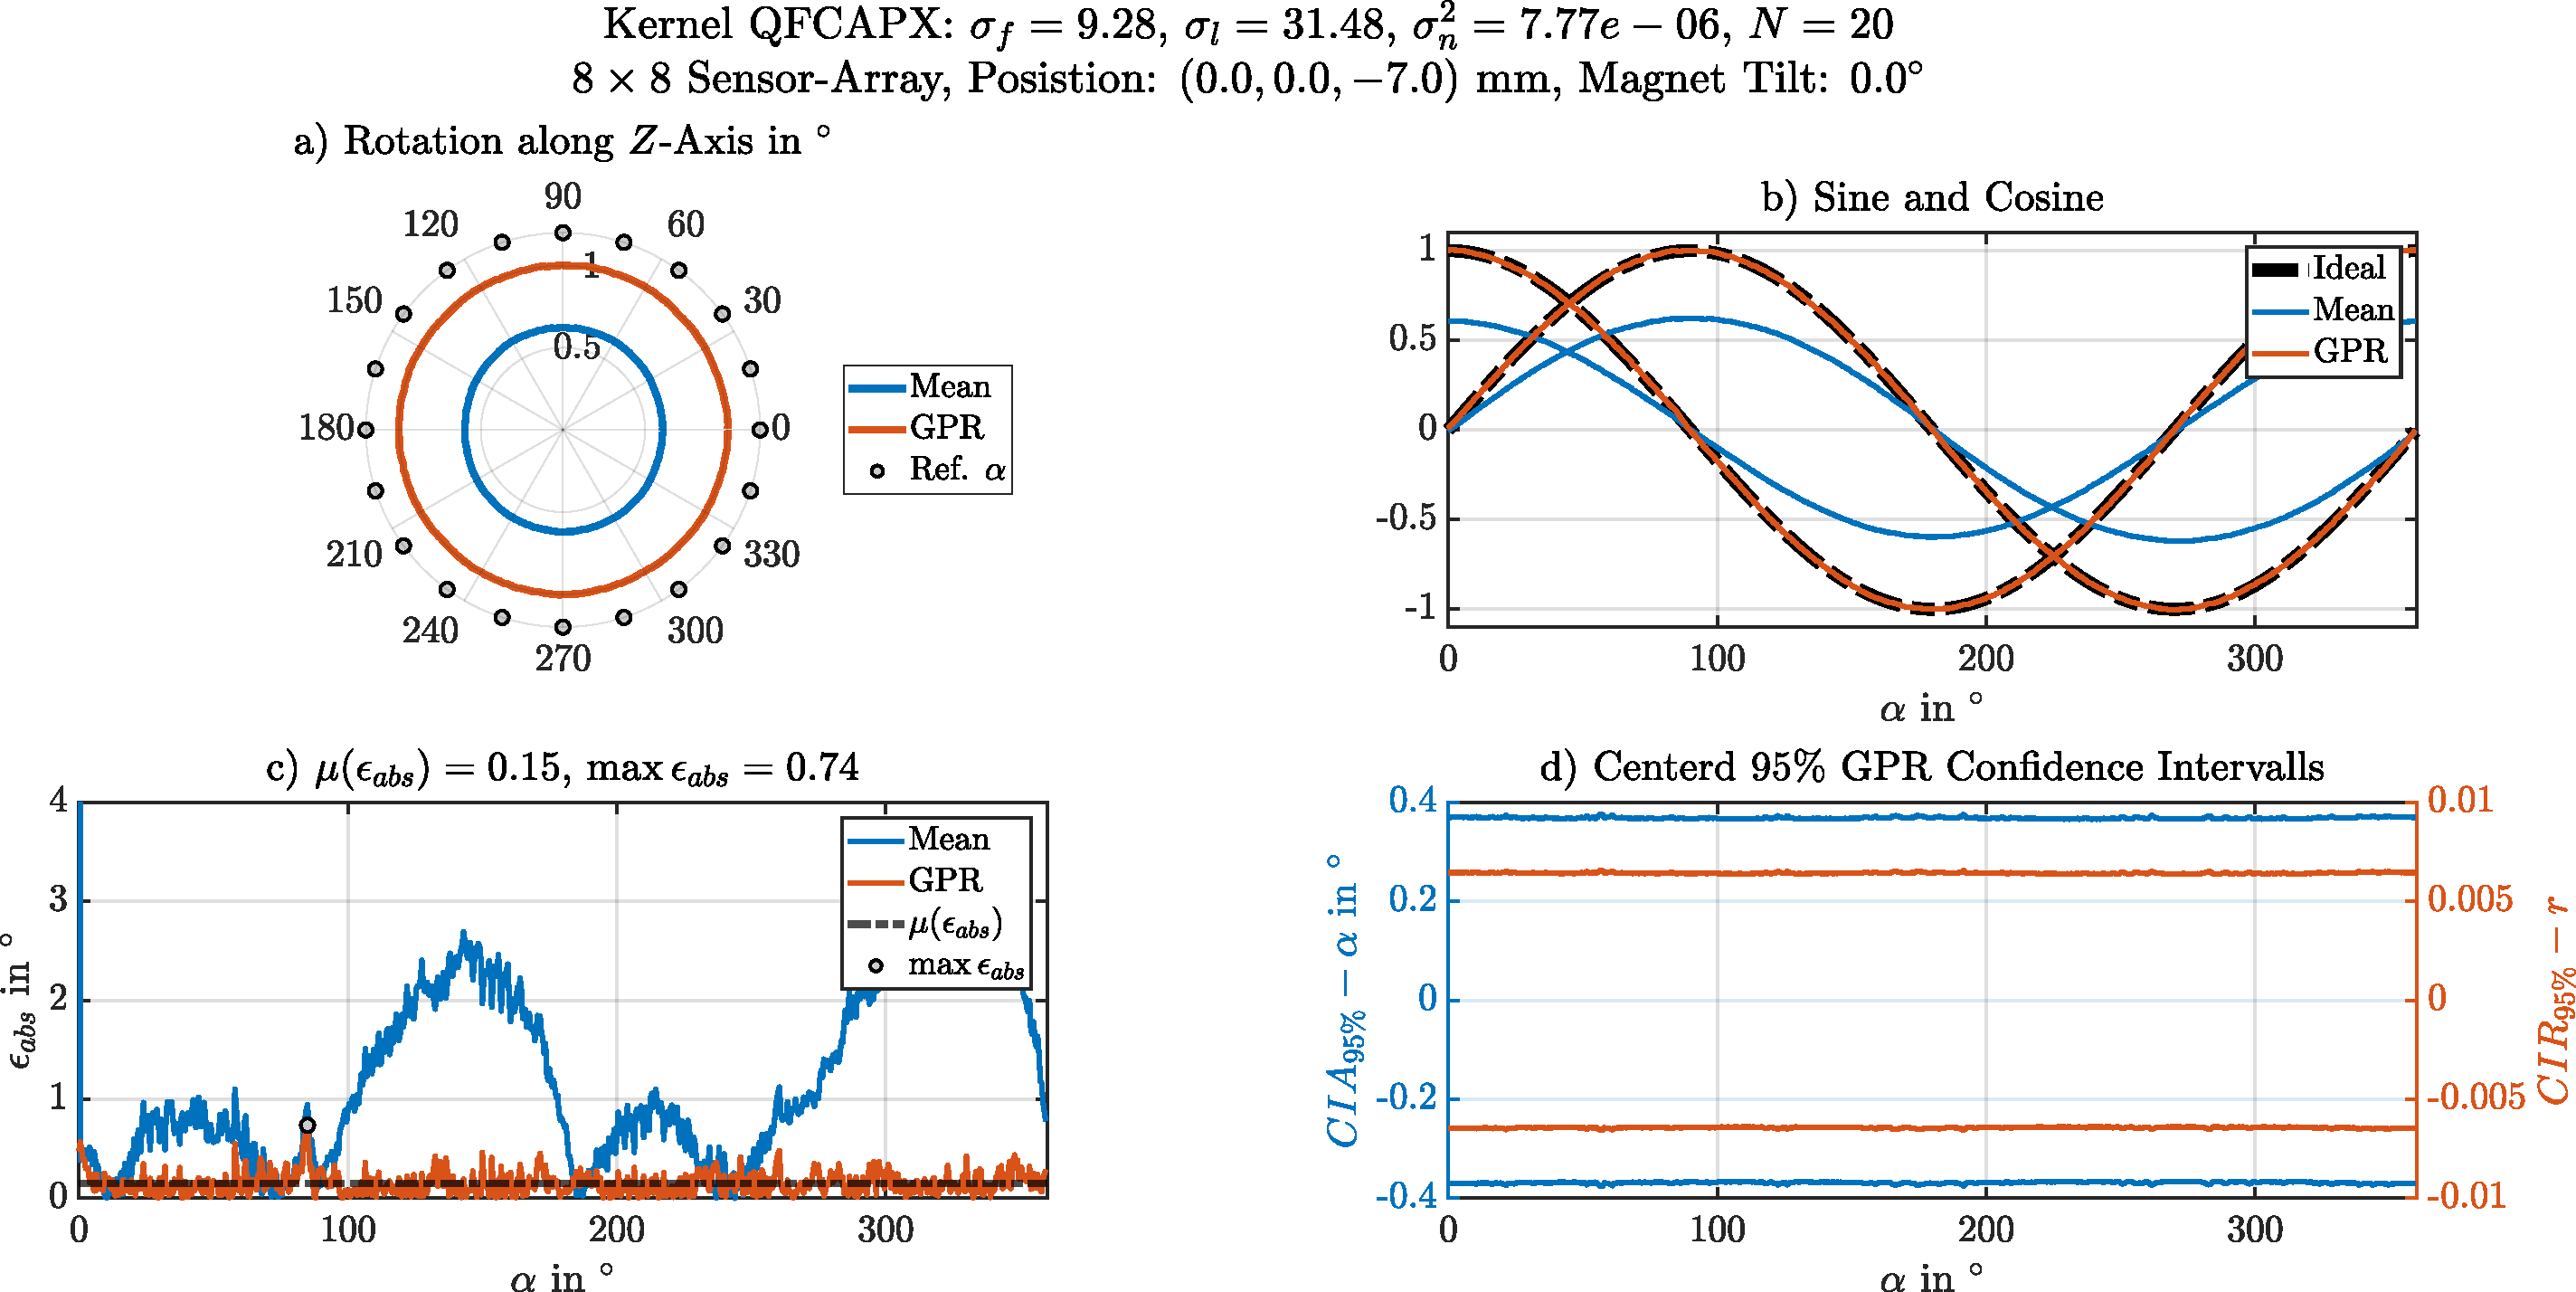
\includegraphics[width=0.9\linewidth]{images/Rotation}
\end{figure}
\begin{columns}[c]
	\column{.45\textwidth}
	\begin{itemize}
		\item<1-> 20 Referenzwinkel
		\item<2-> 720 Winkel, $\SI{0,5}{\degree}$ Auflösung
	\end{itemize}
	
	\column{.45\textwidth}
	\begin{itemize}
		\item<3-> Approximierter Kernel (1)
		\item<4-> Konfidenzintervall konst.
	\end{itemize}
\end{columns}
\end{frame}
%%%%%%%%%%%%%%%%%%%%%%%%%%%%%%%%%%%%%%%%%%%%%%%%%%%%%%%%%%%%%%%%%%%%%%%%%%%%%%%%%%%%%%%%%%%%%%%%%%%%%%%%%%%%%%%%%%%%%%%%%%%%%%%%%%%%%%%%%

\begin{frame}
\Huge{\centerline{Vielen Dank!}}
\end{frame}

%----------------------------------------------------------------------------------------

\begin{frame}
\begin{figure}
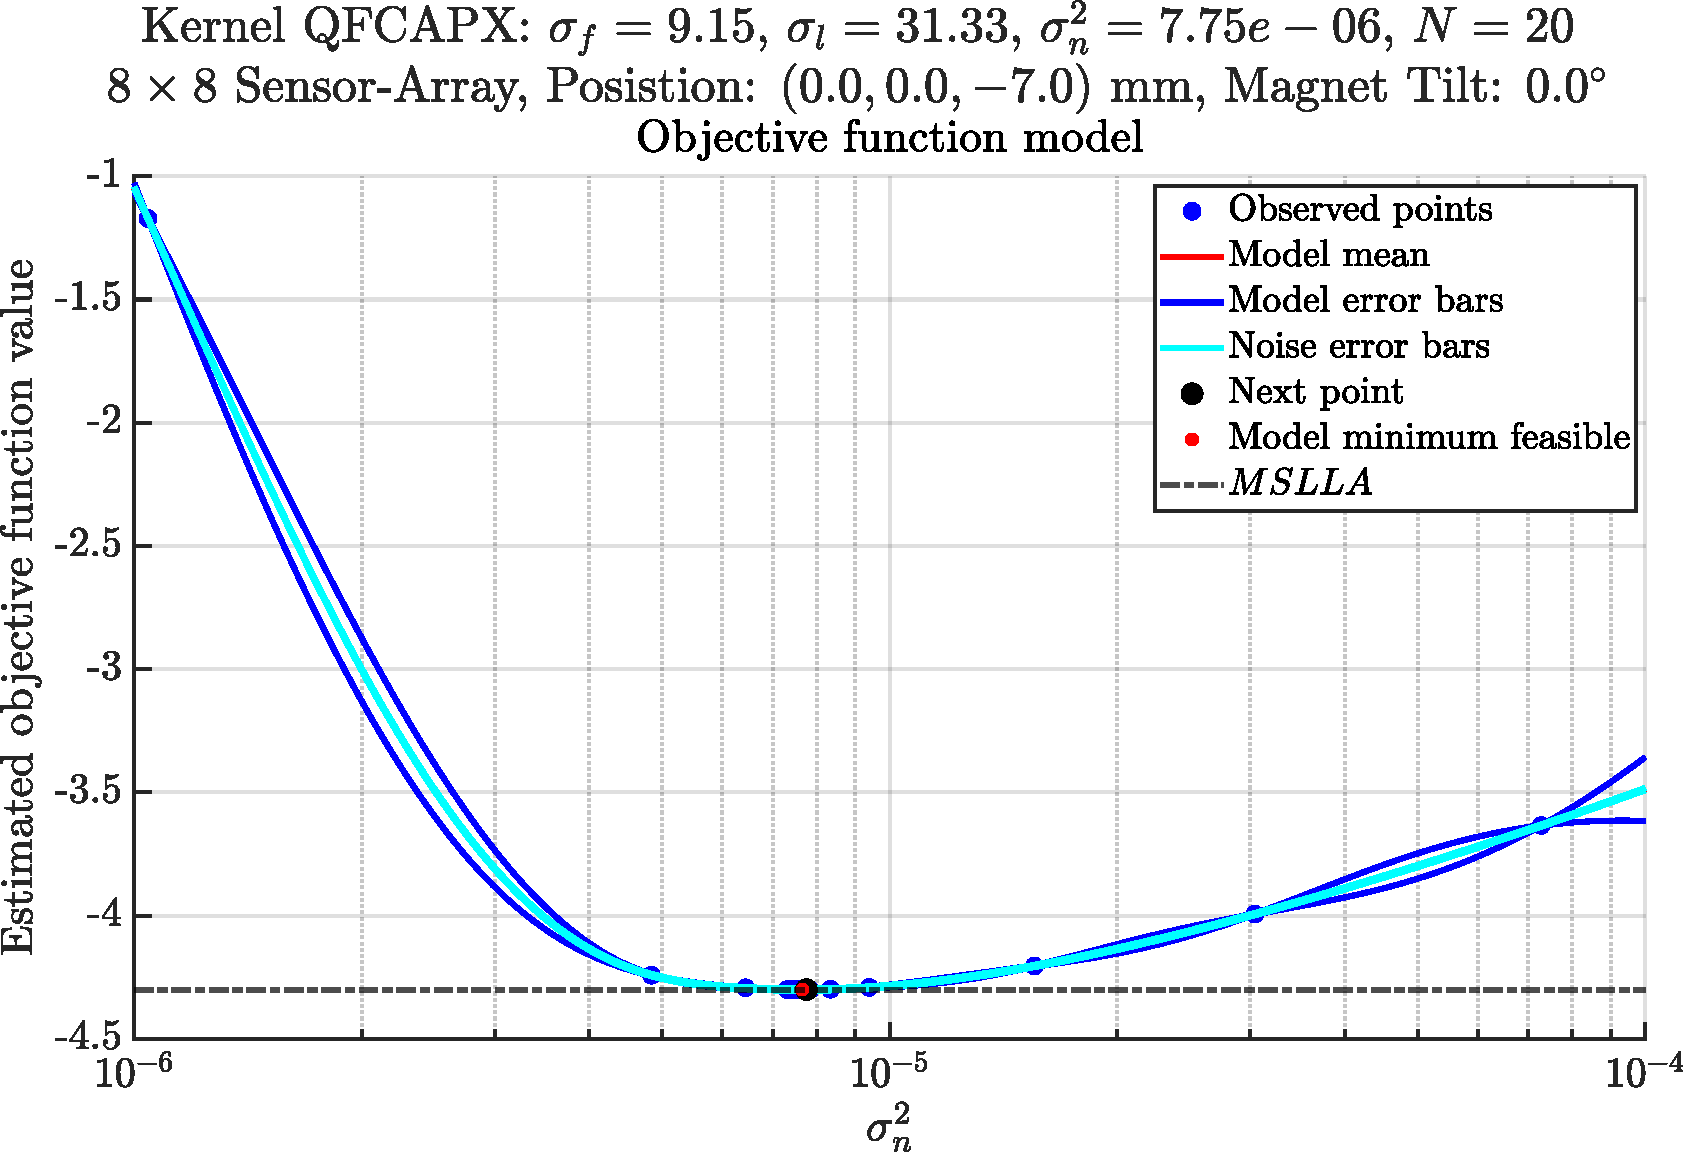
\includegraphics[width=\linewidth]{images/bayes-opt}
\end{figure}
\end{frame}

\begin{frame}
\begin{figure}
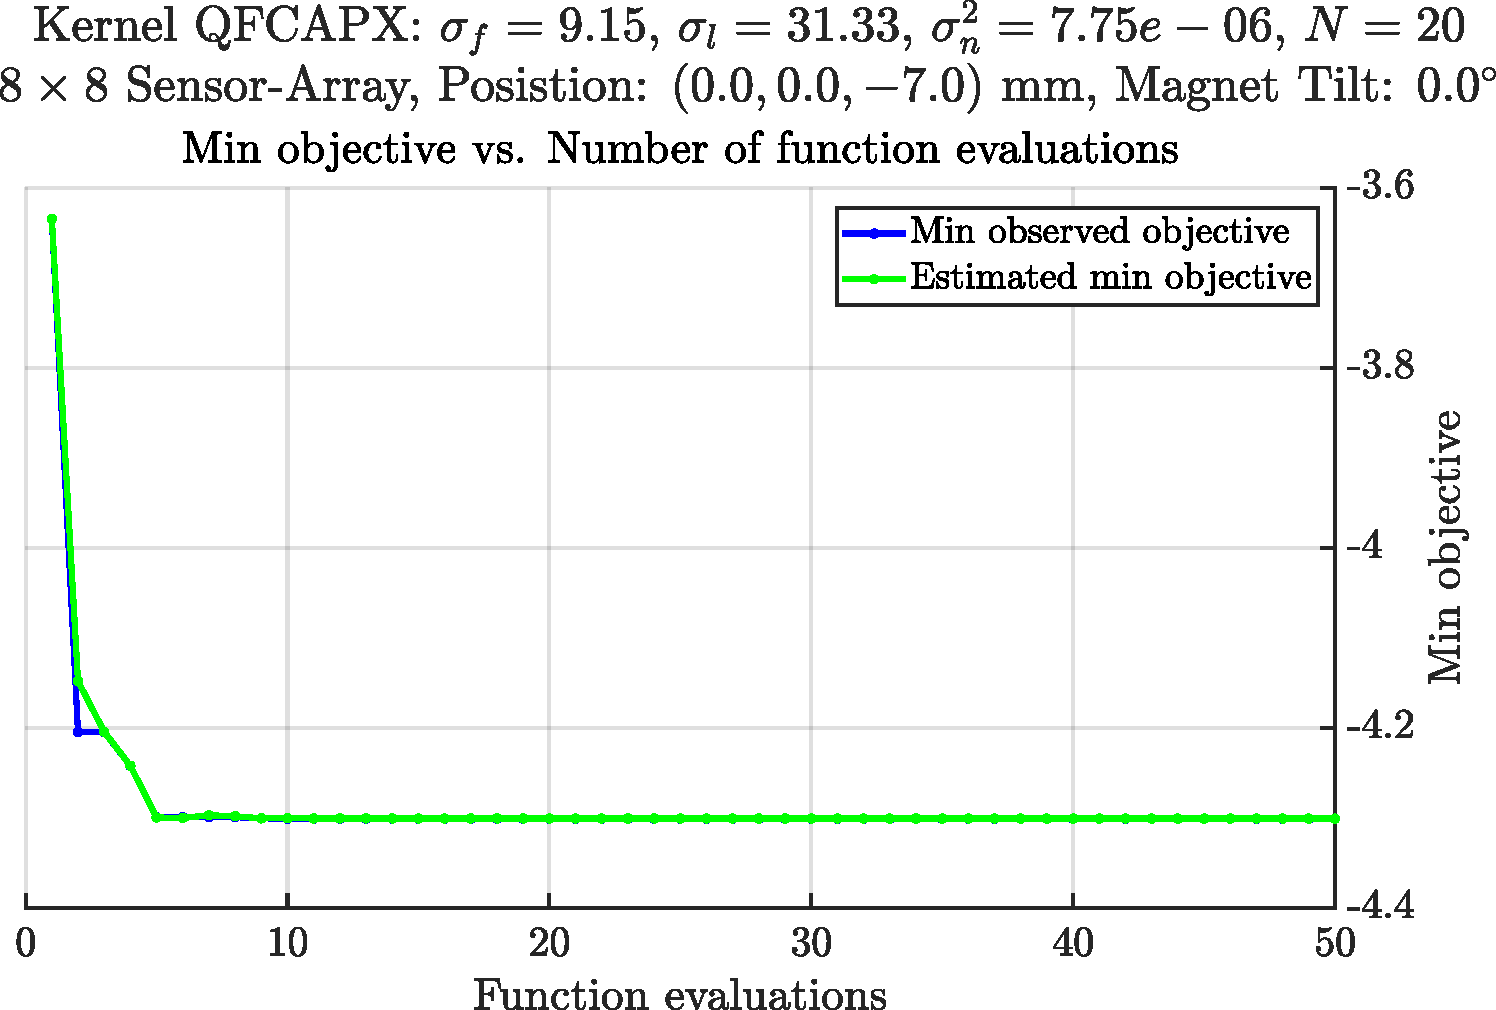
\includegraphics[width=\linewidth]{images/bayes-runs}
\end{figure}
\end{frame}

\begin{frame}
\begin{figure}
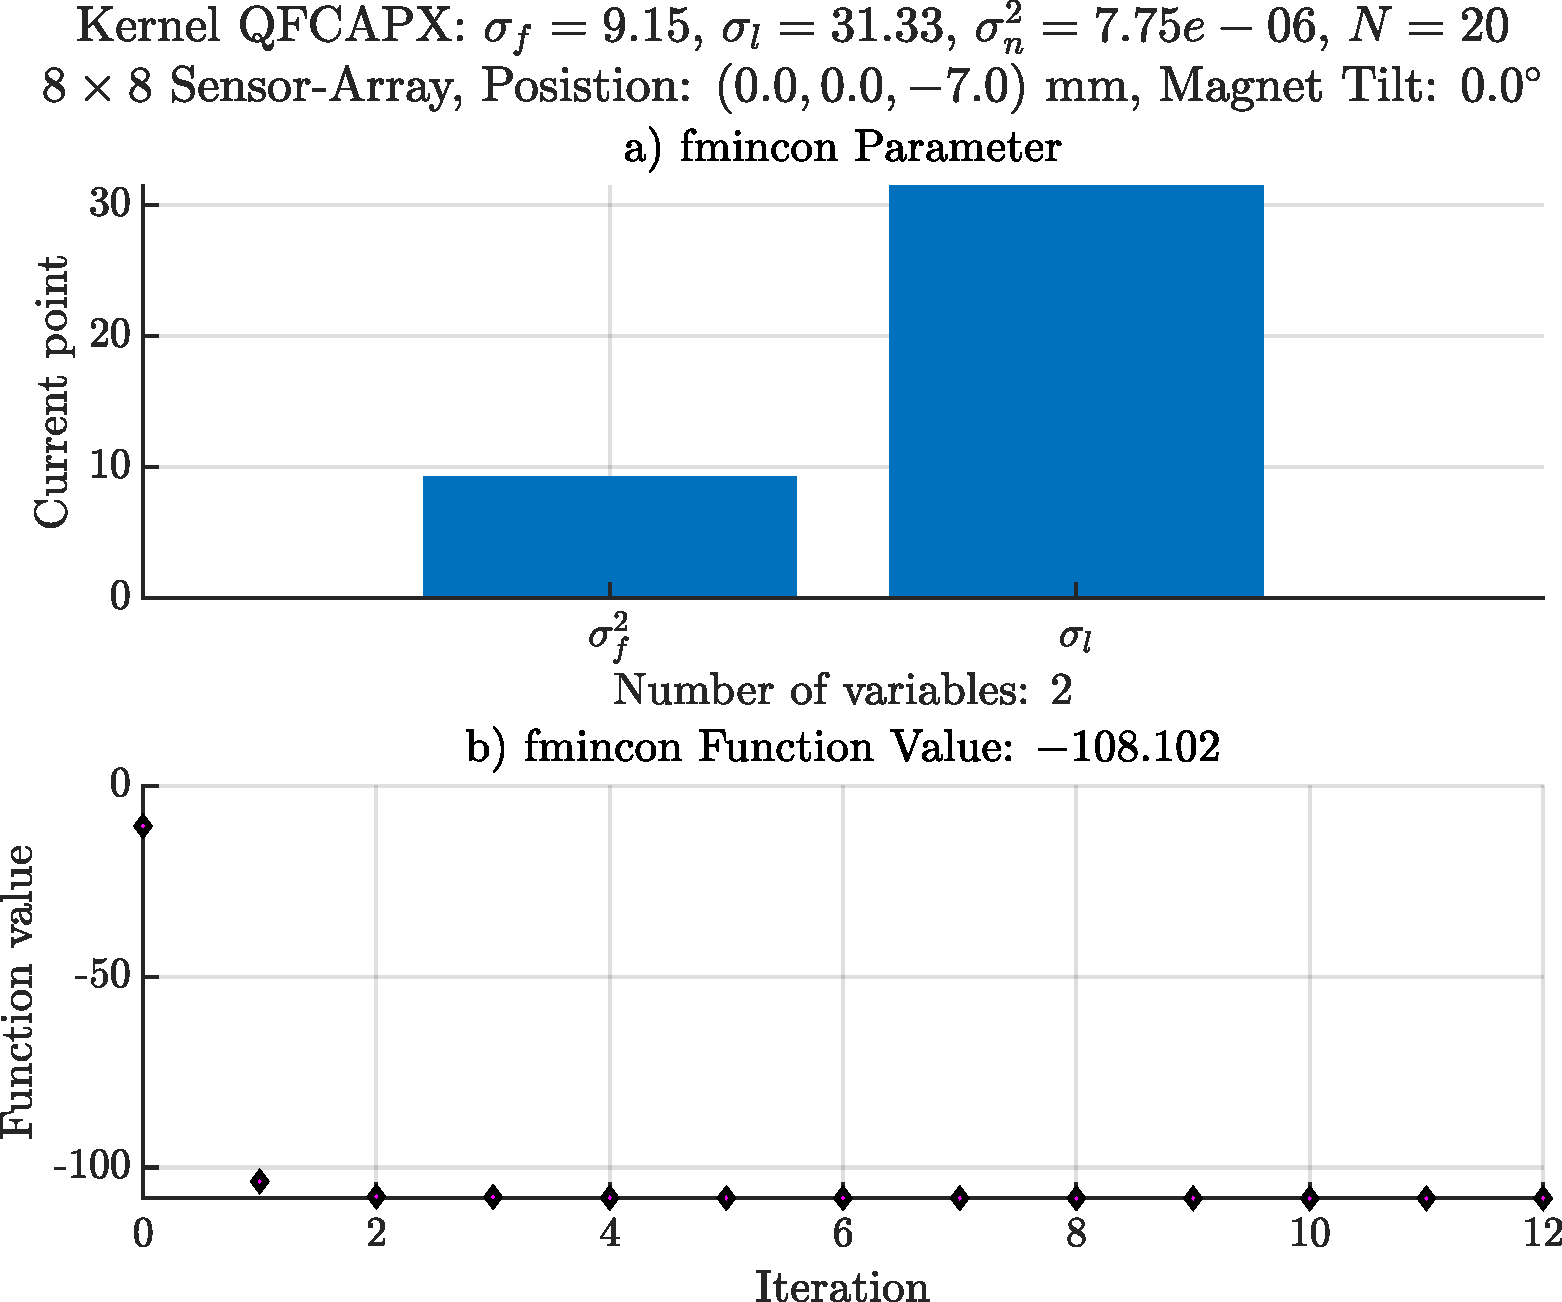
\includegraphics[width=.8\linewidth]{images/fmincon_tuning}
\end{figure}
\end{frame}

\begin{frame}
\begin{figure}
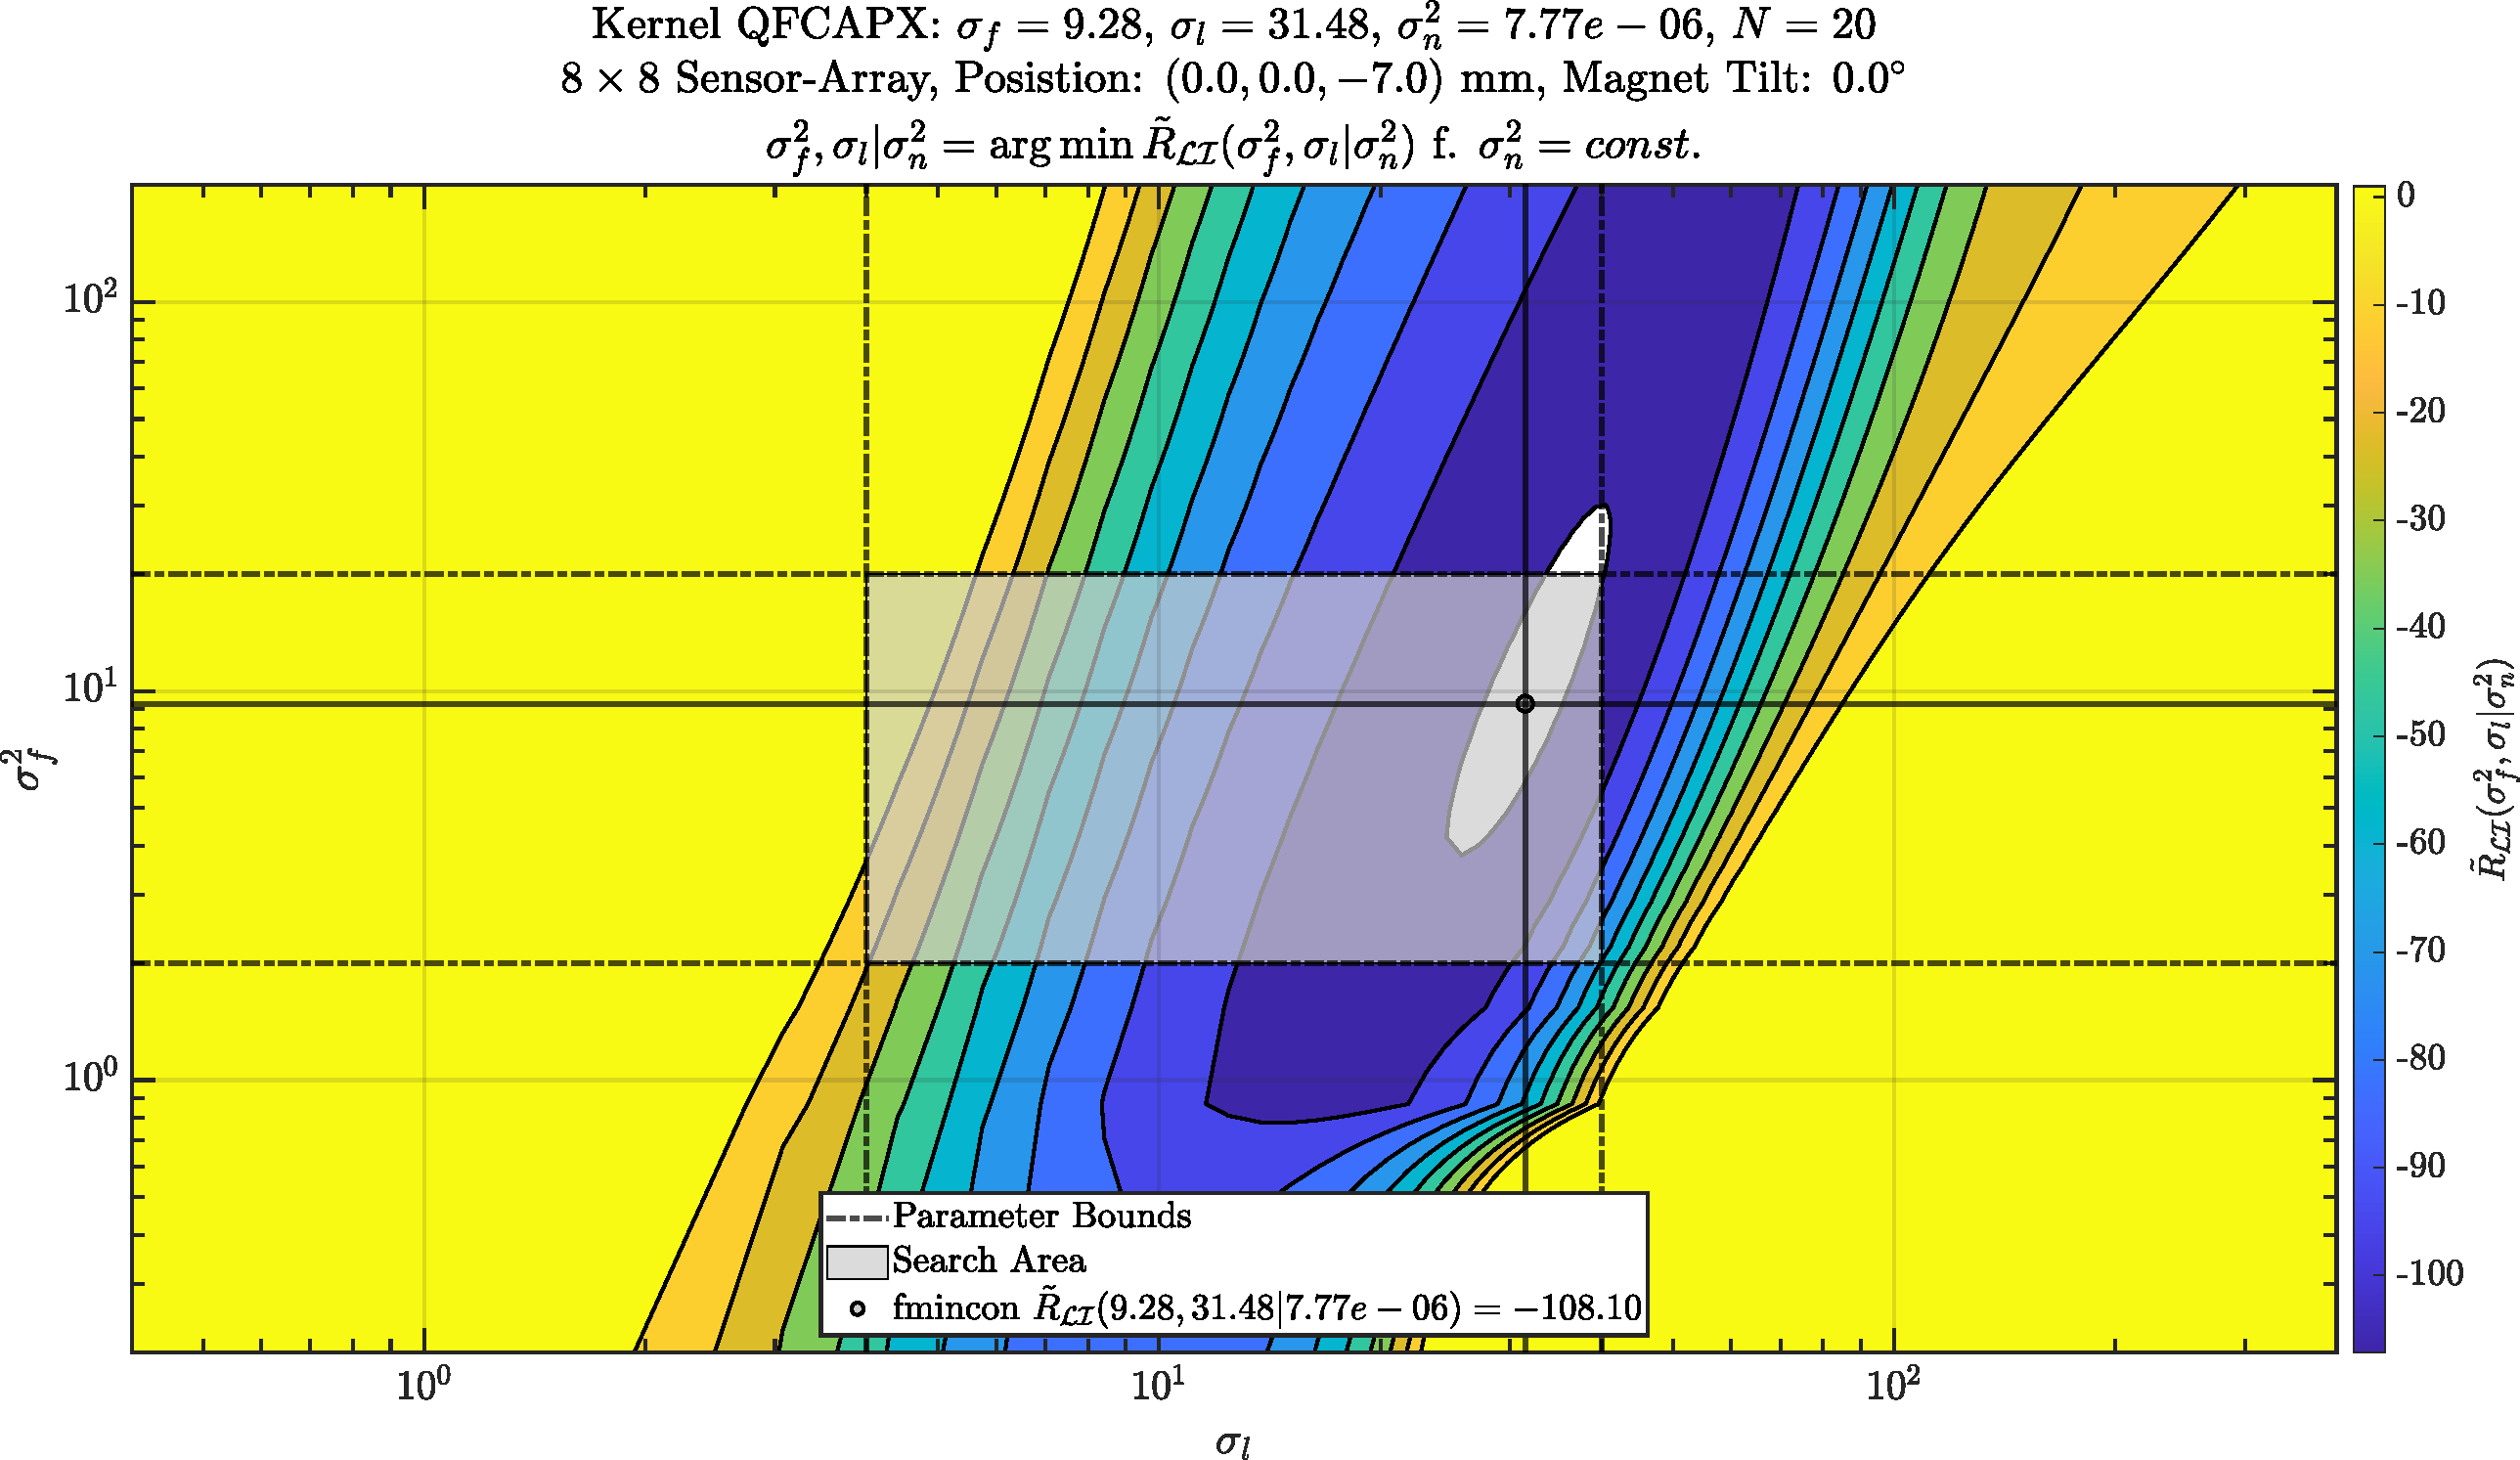
\includegraphics[width=\linewidth]{images/Variance_vs_Length}
\end{figure}
\end{frame}

\begin{frame}
\begin{figure}
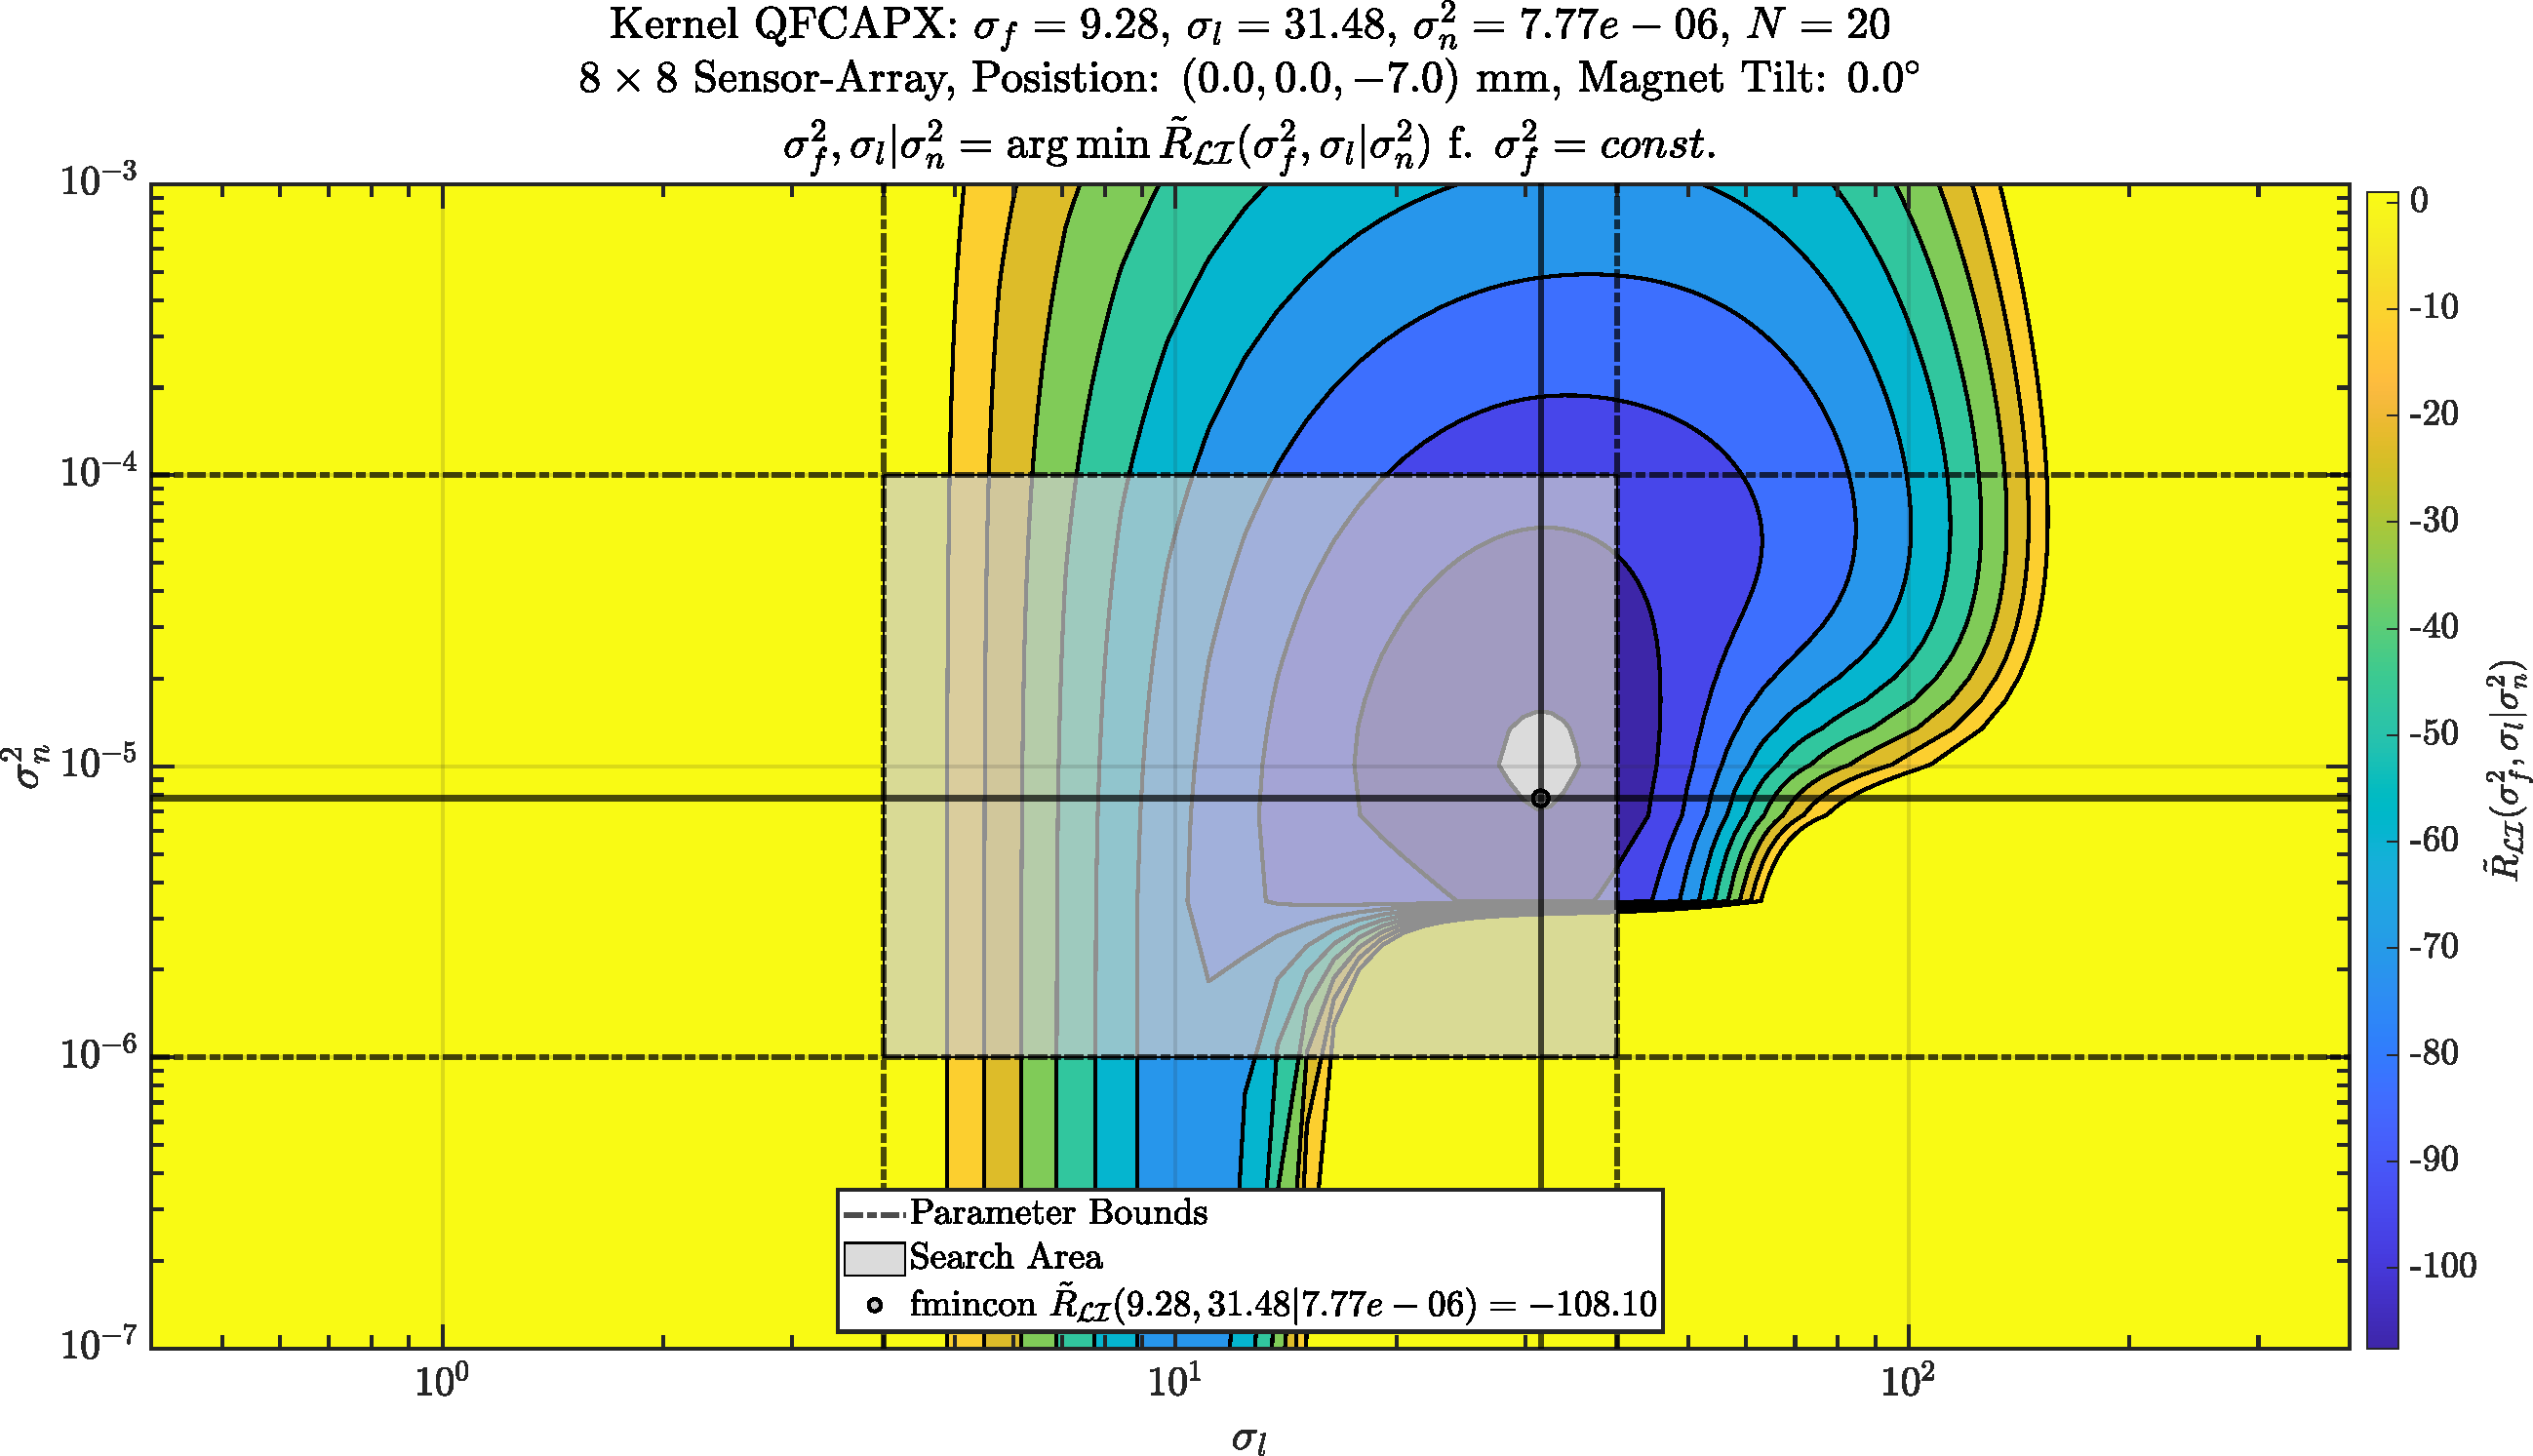
\includegraphics[width=\linewidth]{images/Noise_vs_Length}
\end{figure}
\end{frame}

\begin{frame}
\begin{figure}
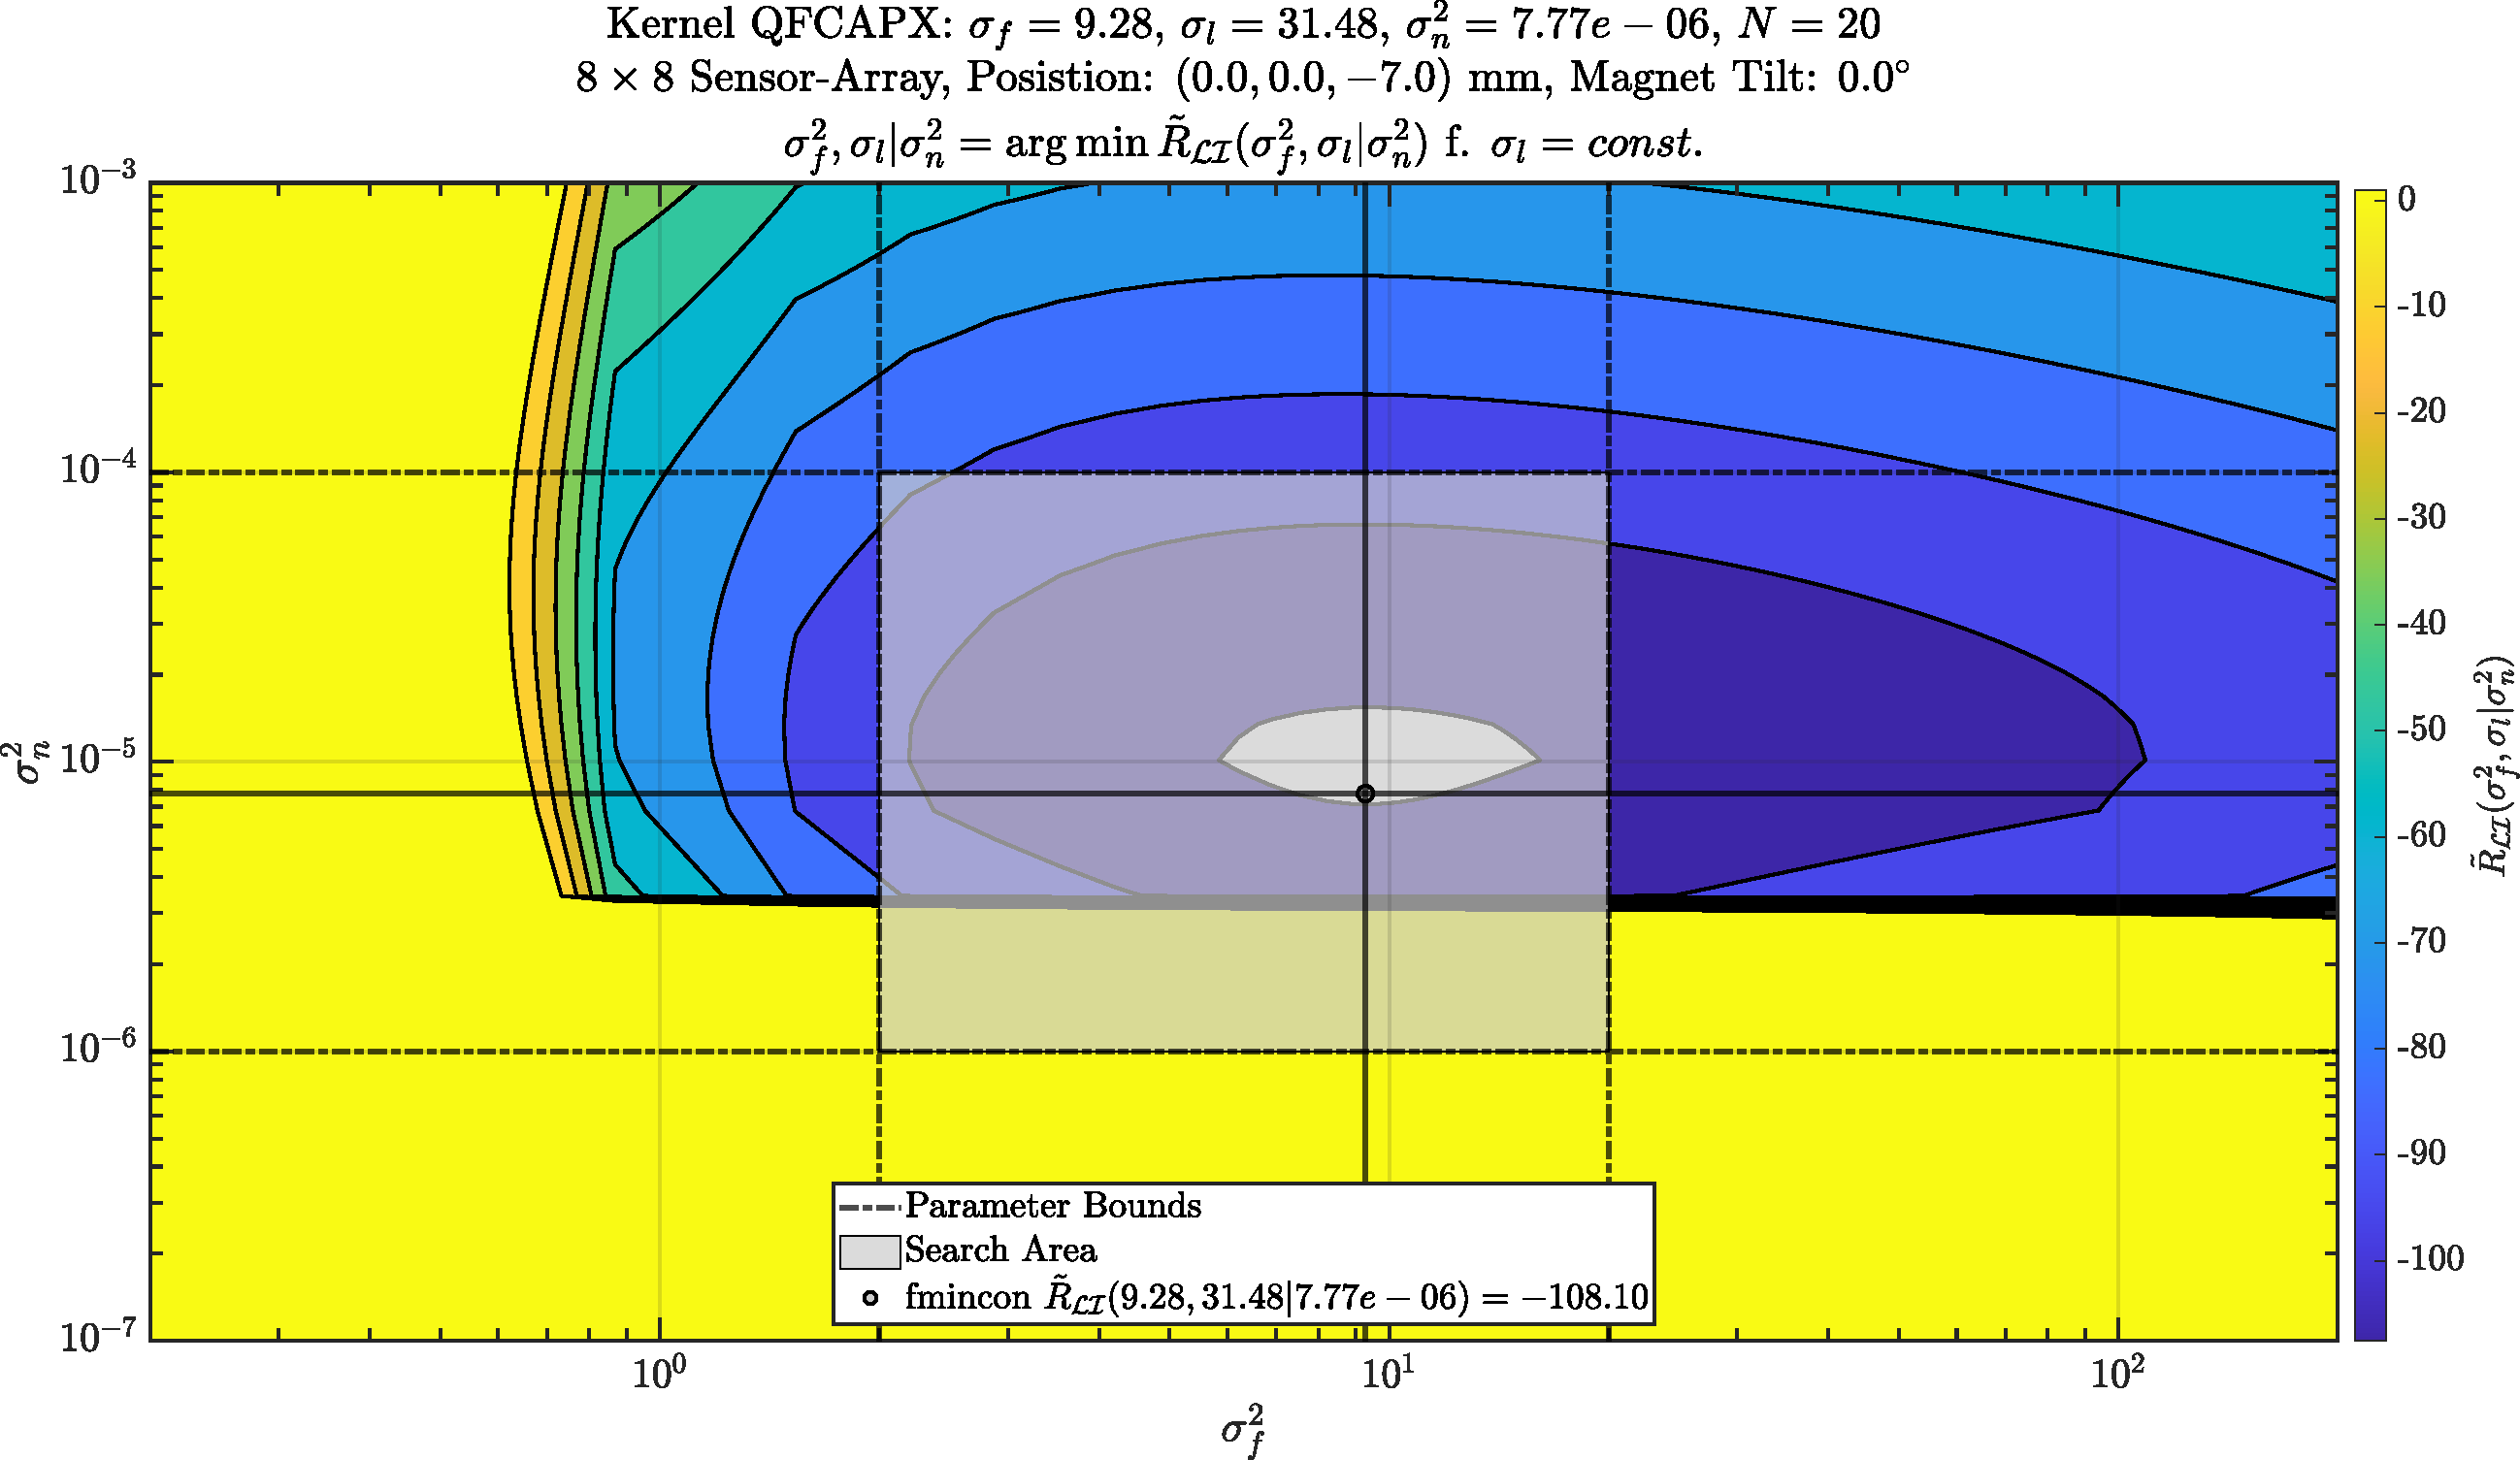
\includegraphics[width=\linewidth]{images/Noise_vs_Variance}
\end{figure}
\end{frame}


\end{document} 